\documentclass[semcabeco,showtrims,12pt,conselho,spreadimages]{memoir}

\usepackage[largepost]{hedraoptions} %% << %%%%%%%%%%%%%%%%
\usepackage[baruch]{hedrastyles}
\usepackage[xetex,chicagofootnotes]{tipografia}
\usepackage[standart,sempontinhos]{toc}
\usepackage{hedraextra}
\usepackage{penalidades}
\usepackage{graficos}
\usepackage{hedralogo}
\usepackage{hifensextras}
\usepackage{fichatecnica}
\usepackage[standart]{aparatos}
\usepackage{tabelas}
\usepackage{versos}
\usepackage{gitrevisioninfo}
\usepackage{parallel}


\newcommand{\forceindent}{\leavevmode{\parindent=1,4em\indent}}

\linespread{1.15}

\newcommand{\paragraphbr}[1]{\vfill\pagebreak\paragraph{#1}}
\renewcommand\theparagraph{\Roman{paragraph}}
\newcommand{\quebra}{\vfil\pagebreak}

%\usepackage{endnotes}
%\renewcommand{\notesname}{Notas}

%\usepackage{fancyhdr}
%\pagestyle{fancy}
%\setlength{\headheight}{9mm}
%\fancyhf{}
%\fancyhead[R]{\thepage}
%\renewcommand{\headrulewidth}{0pt}

%\lhead[\fancyplain{}]{}
%\chead[\fancyplain{}]{}
%\rhead[\fancyplain{}]{\cnvt{\thepage} -- \thepage}

%\newcommand*{\cnvt}[1]{\the\numexpr#1-1\relax}

%\fancypagestyle{chapter}{
%\pagestyle{fancy}
%\setlength{\headheight}{5mm}
%\fancyhf{}
%\fancyhead[R]{\thepage}
%\renewcommand{\headrulewidth}{0pt}}


%\usepackage{footmisc}

%\renewcommand*\footnoterule{}
%\fancyhf[RO]{\cnvt{\thepage} -- \thepage}
%\fancyfoot{}
%\renewcommand{\headrulewidth}{0pt}
%\renewcommand{\footrulewidth}{0pt}}

\usepackage{fontspec}

%\usepackage{Formular}
\newfontfamily\Formular{Formular-Regular}[
BoldFont = Formular-Bold.otf]	

%--------------------------------------------ALTERAR DISTÃNCIA ENTRE TÍTULO DO SUMÁRIO E CAPÍTULOS
%\addtocontents{toc}{\vskip-15pt}
%--------------------------------------------
\usepackage{afterpage}

\newcommand\blankpage{%
    \null
    \thispagestyle{empty}%
    \addtocounter{page}{0}%
    \newpage}

%\usepackage{imakeidx} 
%\makeindex[program=xindy, options=-C utf8 -L portuguese]
%\newcommand\gobbleone[1]{}
%\newcommand*{\seeonly}[2]{\ (\emph{\seename} #1)}
%\newcommand*{\also}[2]{\emph{cf.} #1}
%\newcommand{\Also}[2]{\emph{See also} #1}
%\renewcommand\indexname{Índice onomástico}
%\makeindex[intoc]

\setcounter{tocdepth}{0}
\setcounter{secnumdepth}{-2} 
%\renewcommand \thesection {\thechapter.\Roman\c@section}
\renewcommand{\thesection}{\arabic{section}}


%\linespread{1.08}
\usepackage{commands}

\usepackage{setspace}

\makeatletter
\newenvironment{Parskip}{%
   \par
   \parskip=0.3\baselineskip \advance\parskip by 0pt plus 2pt
   \parindent=\z@
   \def\@listI{\leftmargin\leftmargini
      \topsep\z@ \parsep\parskip \itemsep\z@}
   \let\@listi\@listI
   \@listi
   \def\@listii{\leftmargin\leftmarginii
      \labelwidth\leftmarginii\advance\labelwidth-\labelsep
      \topsep\z@ \parsep\parskip \itemsep\z@}
   \def\@listiii{\leftmargin\leftmarginiii
       \labelwidth\leftmarginiii\advance\labelwidth-\labelsep
       \topsep\z@ \parsep\parskip \itemsep\z@}
   \partopsep=\z@
}{\par}
\makeatother

\makeatletter
\newenvironment{myParskip}{%
   \par
   \parskip=0.2\baselineskip \advance\parskip by 0pt plus 2pt
   \parindent=\z@
   \def\@listI{\leftmargin\leftmargini
      \topsep\z@ \parsep\parskip \itemsep\z@}
   \let\@listi\@listI
   \@listi
   \def\@listii{\leftmargin\leftmarginii
      \labelwidth\leftmarginii\advance\labelwidth-\labelsep
      \topsep\z@ \parsep\parskip \itemsep\z@}
   \def\@listiii{\leftmargin\leftmarginiii
       \labelwidth\leftmarginiii\advance\labelwidth-\labelsep
       \topsep\z@ \parsep\parskip \itemsep\z@}
   \partopsep=\z@
}{\par}
\makeatother

\newcommand{\mystar}{{\fontfamily{lmr}\selectfont$\star$}}

%\makeatletter
%\renewcommand{\@chapapp}{}% Not necessary...
%\newenvironment{chapquote}[2][2em]
%  {\setlength{\@tempdima}{#1}%
%   \def\chapquote@author{#2}%
%   \parshape 1 \@tempdima \dimexpr\textwidth-2\@tempdima\relax%
%   \itshape}
%  {\par\scriptsize\hfill-- \chapquote@author\hspace*{\@tempdima}\par\bigskip}
%\makeatother

%\newcommand\Chapter[2]{\chapter
%  [#1\hfil\hbox{}\protect\linebreak{\itshape#1}]%
%  {#1\\[2ex]\Large\itshape#2}%
%}

\begin{document}
%%!TEX root=./LIVRO.tex

\part{\textsc{mare nostrum: paranã tipi}}
\movetooddpage
\begin{absolutelynopagebreak}
\begin{vplace}
\begin{figure}[H]
\begin{adjustwidth}{-1.8cm}{}
  %\centering
  \vspace*{-2.6cm}
  %\hspace{-0.5cm}
  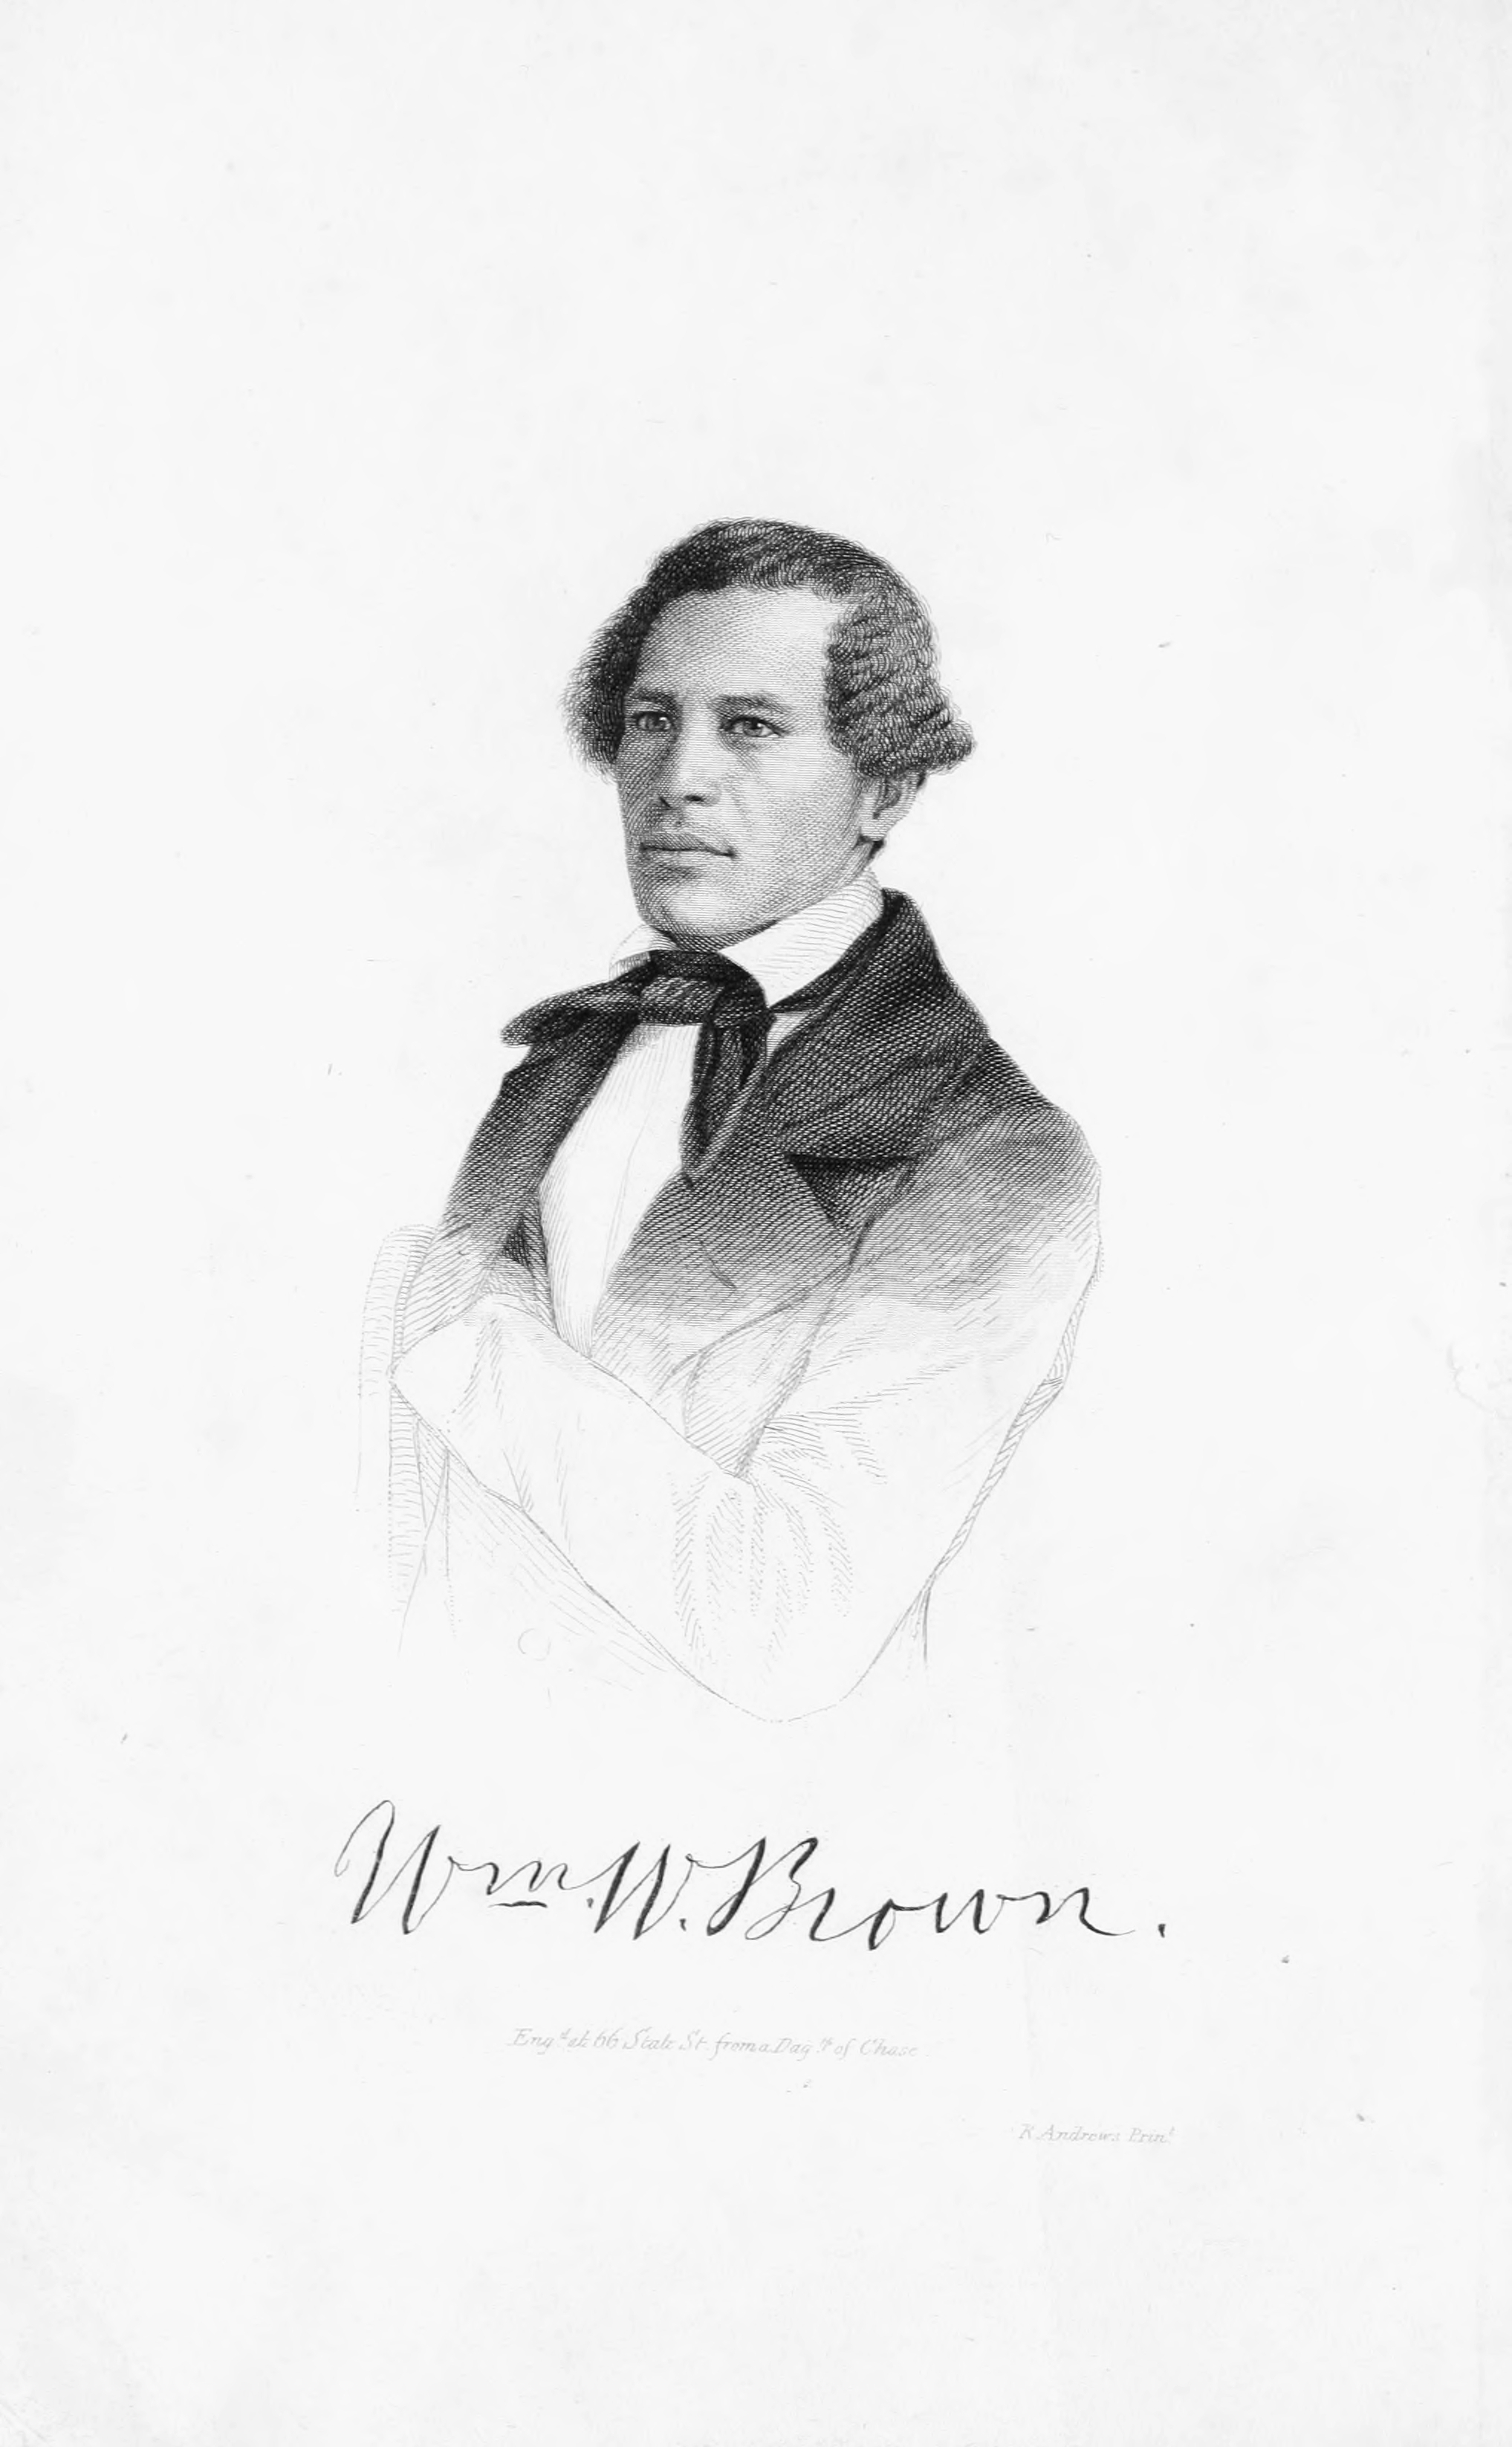
\includegraphics[width=134mm]{./imgs/front1.jpg}  \label{front}
  %\hfill
\end{adjustwidth}
  \caption{}
\end{figure}
\end{vplace}

\thispagestyle{empty}
\end{absolutelynopagebreak}


\pagebreak

\begin{absolutelynopagebreak}
\begin{vplace}
\begin{figure}[H]
\begin{adjustwidth}{-1.8cm}{}
  %\centering
  \vspace*{-2.6cm}
  %\hspace{-0.5cm}
  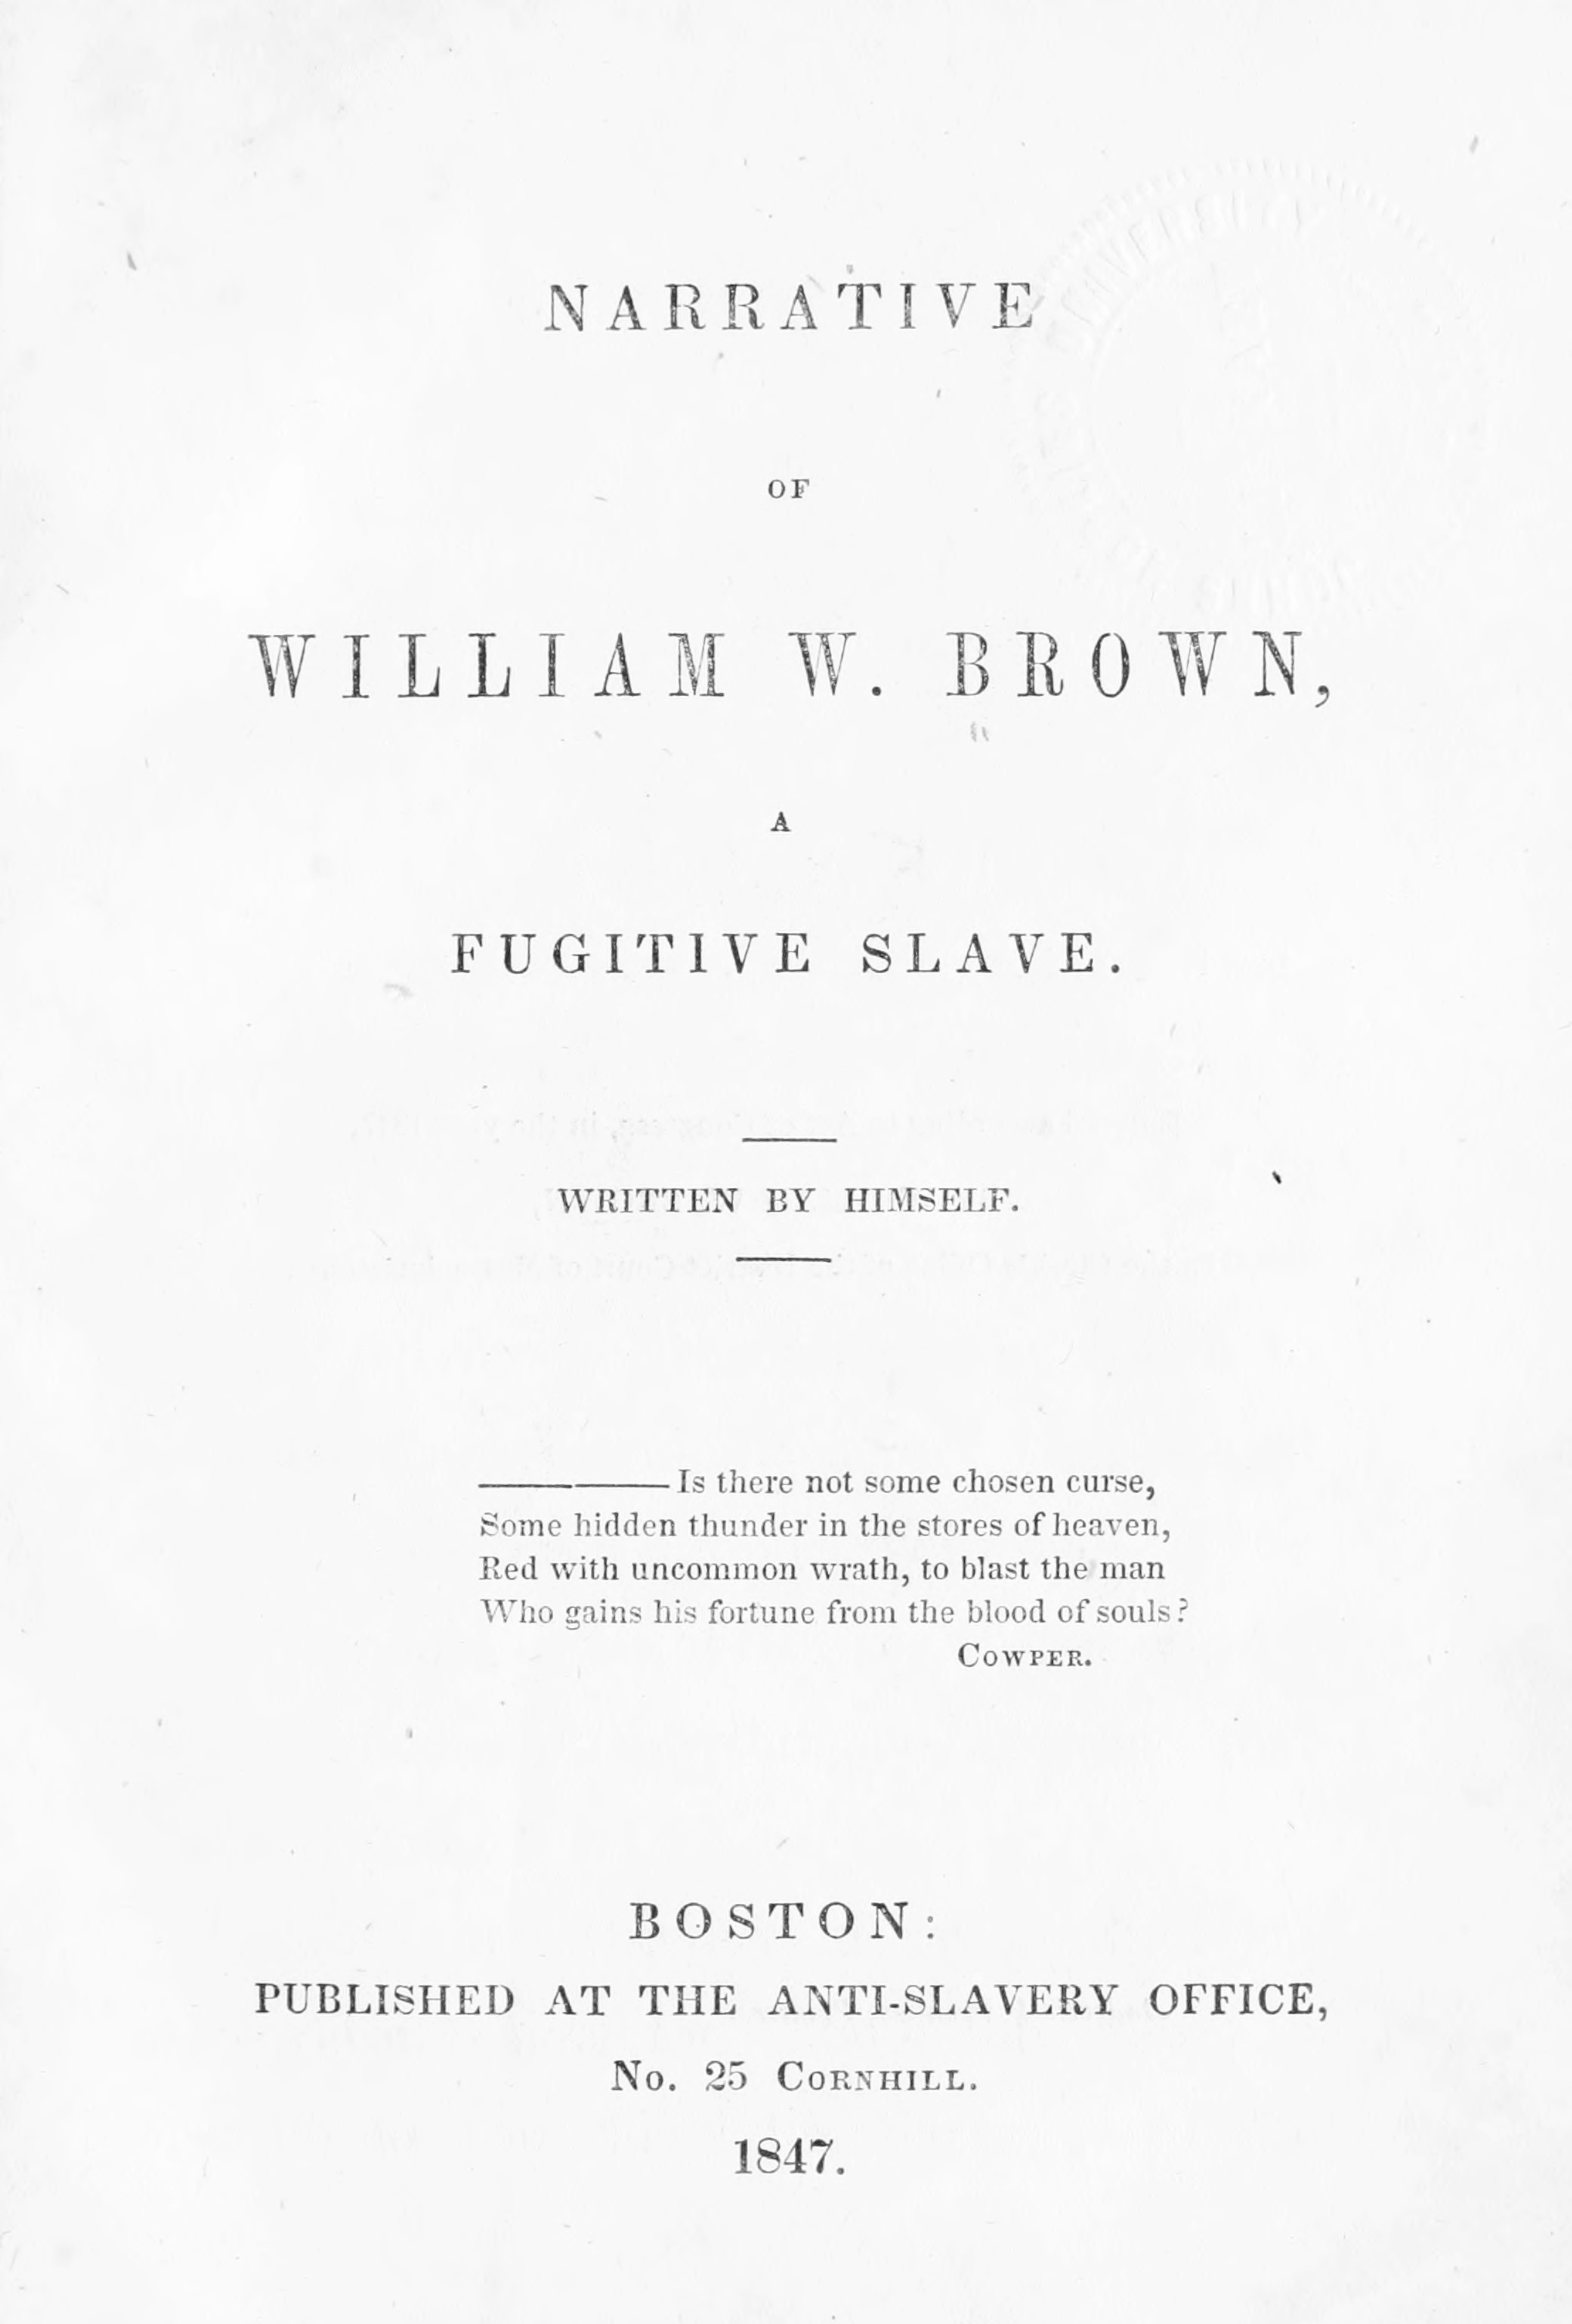
\includegraphics[width=134mm]{./imgs/front2.jpg}  
  %\hfill
\end{adjustwidth}
  \caption{Frontispício da primeira edição da autobiografia de William Wells Brown, publicada em Boston em 1847.}
\end{figure}
\end{vplace}

\thispagestyle{empty}
\end{absolutelynopagebreak}


\movetooddpage
\addcontentsline{toc}{part}{Narrativa de William Wells Brown}
\part*{Narrativa de William Wells Brown, escravo fugitivo, escrita por ele mesmo}


\chapter*{}
\thispagestyle{empty}
\begin{verse}
---Is there not some chosen curse,\\
Some hidden thunder in the stores of heaven,\\
Red with uncommon wrath, to blast the man\\
Who gains his fortune from the blood of \qb{}souls?\footnote{Tradução: ``Não haveria uma maldição seleta/ Um trovão oculto no arsenal celeste,/ Rubro com fúria especial, para fulminar o homem/ Que faz sua fortuna com o sangue das almas?''}
\end{verse}
\begin{flushright}
\versal{COWPER}\footnote{Brown atribui esses versos ao poeta inglês William
  Cowper (1731--1800). Na verdade, a passagem pertence à peça \emph{Cato,
  A Tragedy}, de Joseph Addison (1672--1719).}
\end{flushright}

\chapter{Para Wells Brown, de Ohio}

Treze anos atrás eu batia à sua porta, cansado, fugindo dos grilhões e
da chibata. Era forasteiro e você me hospedou. Estava faminto e você me
deu de comer. Estava nu e você me deu de vestir. A escravidão me negara
até um nome pelo qual pudesse ser chamado entre os homens, e você me deu
o seu. Eu seria uma criatura deveras vil se esquecesse tudo que te devo 
ou fizesse o que fosse para desonrar o seu nome sagrado!

Como pequeno testemunho da gratidão que tenho pelo meu primeiro
benfeitor, tomo a liberdade de lhe dedicar esta pequena \emph{Narrativa} dos
sofrimentos dos quais estava fugindo quando fui agraciado com a sua
compaixão. Entre as multidões que receberam seu auxílio, é bem possível
que você não se lembre de mim; mas até que eu esqueça Deus e a mim
mesmo, nunca me esquecerei de você.

Teu amigo agradecido

\begin{flushright}
\emph{William Wells Brown}
\end{flushright}

\chapter{Carta de Edmund Quincy} %, esq.

\begin{flushright}
\emph{Dedham, 1º de julho de 1847}
\end{flushright}

\begin{flushleft}
Para William Wells Brown
\end{flushleft}

Meu caro amigo: Agradeço sinceramente pelo privilégio de ler o
manuscrito da sua \emph{Narrativa}. Li"-a com profundo interesse e fiquei
emocionado. Tenho certeza que será, além de um enorme sucesso, de
extrema utilidade. Ela apresenta uma fase diferente do sistema
escravista infernal em relação àquela retratada na história admirável do
Sr.\,Douglass\footnote{Frederick Douglass (1819--1895): Abolicionista,
  jornalista e político americano. Sua primeira autobiografia, a
  \emph{Narrativa da vida de Frederick Douglass, um escravo americano},
  foi um sucesso de vendas na época e ainda é considerada um clássico da
  literatura dos \versal{EUA}.} e nos permite vislumbrar as crueldades atrozes de
outras partes do seu domínio.

As oportunidades que você teve de observar o funcionamento desse sistema
maldito foram particularmente grandes. Suas experiências na Lavoura, na
Casa Grande e, especialmente, no Rio, a serviço de Walker, o traficante
de escravos, quase não encontra paralelo entre outros indivíduos, e
certamente nenhum que tenha demonstrado a competência para descrevê"-los.
O que admiro, e o que me assombra, na sua \emph{Narrativa} é a calma e a
simplicidade com que descreve cenas e ações que poderiam muito bem
``levar as próprias pedras a se erguerem em motim'' contra a Instituição
Nacional que as tornam possíveis.

Como irá perceber, em muito pouco fiz uso da gentil permissão que me deu
para alterar aquilo que escreveras. Corrigir alguns equívocos, que \label{ref1}
pareciam ser meros erros de cópia, cometidos na pressa da composição,
empreendida em condições desfavoráveis, e sugerir alguns abreviamentos,
foi tudo que ousei fazer. Seria muita audácia da minha parte, e muita
vaidade também, tentar melhorar as descrições do que você viu e sofreu.
Algumas das cenas fariam jus ao próprio De Foe.

Confio que sua narrativa terá ampla circulação e tenho certeza de que
ela o merece. Deve possuir uma natureza diferente da minha o homem que
encerre a leitura da \emph{Narrativa} sem acreditar que entende a escravidão
melhor do que nunca, e a odeie ainda mais.

Fiel e respeitosamente, 

Seu amigo

\begin{flushright}
\emph{Edmund Quincy}
\end{flushright}

\chapter{Prefácio à primeira edição}

Os amigos da liberdade podem comemorar o surgimento da \emph{Narrativa} a
seguir, que acrescenta mais um volume à crescente literatura
antiescravista contemporânea. Como afirmou um grande observador da
natureza humana: ``Deixem"-me compor as canções de uma nação e não me
importarei com quem compõe suas leis'';\footnote{Frase de Andrew Fletcher
  (1655--1716), escritor e político antiunionista escocês.} e com o
mesmo grau de verdade pode"-se dizer que, entre um povo leitor como o
nosso, nossos livros irão ao menos caracterizar nossas leis. É uma
influência que avança silenciosamente em sua missão, mas jamais deixa de
encontrar o caminho a muitos corações calorosos para acender em seus
altares a chama da liberdade que um dia se conflagrará no incêndio que
há de consumir a opressão.

Este livreto é uma voz emanando da prisão, desvendando os feitos
sombrios que nela são perpetrados. Nossa causa recebe um grande socorro
dessa fonte. Os nomes daqueles que vieram de lá, e que batalharam
valorosamente pela justiça, não precisam ser registrados aqui. As obras
de alguns deles são monumentos eternos à divindade e seu registro
perpétuo encontra espaço nos corações agradecidos dos cativos redimidos.

Poucas pessoas tiveram maior oportunidade para conhecer a escravidão em
todos os seus aspectos mais terríveis do que William W. Brown. Ele
esteve por trás dos panos. Visitou suas câmaras secretas. Os ferros dela
penetraram a sua alma. Os laços mais caros da natureza foram fendidos em
sua pessoa. Uma mãe foi açoitada cruelmente perante seus próprios olhos.
Um pai\ldots{} mas, ah, escravo não tem pai. Um irmão se tornou vítima
de sua própria misericórdia. Uma irmã foi entregue ao controle
irresponsável do pálido opressor. E esta nação assente com a cena. A
União americana sanciona esses feitos. A Constituição protege os
criminosos. A religião americana santifica o crime. Mas a maré está
virando. Uma corrente submarina arrasta o país para a frente. Uma voz de
alerta, de admoestação, de censura, de rogo, está soando. Mãos seguram
mãos e corações se mesclam com corações na grande obra da salvação dos
escravos.

Mesmo agora, as convulsões do monstro evidenciam suas feridas profundas.

O autor desta \emph{Narrativa} foi emprestado pelo seu senhor para um
``\emph{traficante de almas}'' e testemunhou todos os horrores do
tráfico, desde a compra do rebanho humano nos estados criadores de
escravos, que produzem uma cena constante da separação das vítimas dos
seus entes queridos, até a sua venda final no mercado do Sul, para serem
exauridos em sete anos ou entregues à luxúria dos \emph{cristãos}
sulistas.

Muitas cenas pungentes são retratadas explicitamente, mas também com uma
simplicidade e uma engenhosidade que transmitem a certeza sobre a
veracidade da imagem.

Este livro fará muito para desmascarar aqueles que ``se vestiram com o
libré da corte celestial'' a fim de disfarçar a monstruosidade dos seus
atos.

Durante os últimos três anos, o autor dedicou todas as suas energias à
causa antiescravista. Labutando sob todas as deficiências e desvantagens
decorrentes de ter sido educado sob a escravidão, de ter sido sujeitado,
como foi desde nascença, a todos os males e privações inerentes à sua
condição, ainda assim ele seguiu em frente, atraído ao trabalho pelo
amor à liberdade, estimulado pela memória do próprio sofrimento, instado
pela consideração de que mãe, irmãos e irmã ainda agonizavam no
cativeiro ao lado de três milhões de filhos do Nosso Pai, sustentado por
uma fé inabalável na onipotência da verdade e no triunfo final da
justiça, para defender a causa dos escravos, e pela eloquência da sua
sinceridade transmitiu a certeza a muitas mentes e arregimentou a
simpatia e a cooperação de muitos outros em prol da causa.

Seu trabalho se limitou principalmente ao oeste do estado de Nova York,
onde conquistou muitos amigos queridos com seu zelo incansável, sua
energia perseverante, sua fidelidade constante e sua bondade universal.

Leitor, és um abolicionista? O que fizestes pelo escravo? O que fazes
por ele? O que pretendes fazer? Uma grande obra nos espera. Quem há de
ficar parado? Em termos comparativos, este é o grande movimento
humanitário da nossa era, engolindo, por ora, todas as outras questões.
O curso da história humana, obediente às leis imutáveis da nossa
existência, avança rapidamente para uma crise final. Eis a pergunta:

\begin{verse}
Have ye chosen, O my people, on whose \qb{}party ye shall stand,\\
Ere the Doom from its worn sandal shakes \qb{}the dust against our land?\footnote{Tradução: ``Já escolhestes, ó, meu povo, que partido ireis tomar,/ Antes que o Destino de suas sandálias gastas sacuda a poeira contra a
nossa terra?''. Versos de \emph{The Present Crisis}, do poeta
  romântico americano James Russell Lowell (1819--1891). ``Sacudir a
  poeira'' é uma referência a Mateus 10:14 e à antiga prática judaica de
  sacudir a poeira dos pés ao sair de cidades não"-judaicas para indicar
  separação do mundo gentio.}
\end{verse}

Você é cristão? Esta é a realização do Cristianismo prático, e não há
outra forma. O Cristianismo é \emph{prático} em sua própria essência e
natureza. É uma vida que nasce da alma imbuída com o seu espírito. É
amigo da causa missionária? Este é o maior empreendimento missionário de
hoje. Três milhões de \emph{cristãos}, transformados em pagãos pela lei,
anseiam pelas boas novas do Evangelho da liberdade. É amigo da Bíblia?
Vem, então, e nos ajuda a restaurar a vista para esses milhões cujos
olhos foram furados pela escravidão, para que possam enxergar e ler a
Bíblia. Ama Deus, a quem nunca viu? Então manifesta esse amor e devolve
ao irmão que já vistes a sua legítima herança, da qual foi privado por
tanto tempo e com tanta crueldade.

Não é por uma única geração de três milhões que trabalhamos, por mais
sublime que seja tal esforço. É pela humanidade, ao redor do mundo, não só agora, mas por todos os tempos, e por todas as gerações futuras:

\begin{verse}
For he who settles Freedom's principles,\\
Writes the death"-warrant of all tyranny.\footnote{Tradução: ``Pois quem estabelece os princípios da Liberdade/ Redige a sentença de morte
de toda a tirana.'' De \emph{L'Envoi}, poema final de \emph{A
  Year's Life}, o primeiro livro de James Russell Lowell.}
\end{verse}

É um trabalho vasto, um empreendimento glorioso, digno da devoção
inarredável de toda a vida dos grandes e dos bons.

O escravismo e os escravistas devem ser convertidos em seres
ignominiosos e detestáveis. Devem perder sua respeitabilidade e sua
reputação cristã. Devem ser tratados como ``ladrões de homens, culpados
do mais grave roubo e pecadores de primeira ordem''.\footnote{Passagem da
  Disciplina da Igreja Presbiteriana dos \versal{EUA}, adotada em 1794 e
  eliminada em 1816 com a influência crescente dos escravistas na
  Assembleia Geral.} Seus cúmplices mais culpados, na pessoa dos
\emph{apologistas nortistas}, tanto na Igreja quanto no Estado, devem
ser colocados na mesma categoria. Os homens honestos devem ser
convencidos a ver esses crimes com a mesma aversão e desprezo que
destinam aos ladrões e assassinos menos culpados, até que:


\begin{verse}
The common damned shun their society,\\
And look upon themselves as fiends less \qb{}foul.\footnote{Tradução: ``Os condenados comuns rejeitam a sua sociedade/ E se consideram demônios menos atrozes.'' De \emph{The Grave}, do poeta
  escocês Robert Blair (1699--1746).}
\end{verse}

Quando o crime da escravidão receber sua justa sentença, o trabalho
estará completo. E terá chegado o dia glorioso:

\begin{verse}
When man nor woman in all our wide \qb{}domain,\\
Shall buy, or sell, or hold, or be a slave.\footnote{Tradução: ``Quando nem homem nem mulher em nossos vastos domínios/ Há de comprar, ou vender, ou ter, ou ser escravo.'' Paráfrase dos versos finais de \emph{Inscription under the Picture of an Aged Negro"-woman}, do poeta escocês James Montgomery (1771--1854).}
\end{verse}

\bigskip

\begin{flushright}
\emph{J. C. Hathaway}

Farmington, Nova York, 1847.
\end{flushright}



\chapter*{Capítulo I}
\addcontentsline{toc}{chapter}{Capítulo \textsc{i}}

Nasci em Lexington, Kentucky. O homem que me roubou assim que nasci \label{ref5}
registrava o nascimento de todos os bebês que alegava serem de sua
propriedade em um livro que mantinha para esse fim. O nome de minha mãe
era Elizabeth. Ela teve sete filhos, a saber: Solomon, Leander,
Benjamin, Joseph, Millford, Elizabeth e eu. Nenhum de nós tinha o mesmo
pai que o outro. O nome de meu pai, como soube de minha mãe, era George
Higgins. Ele era um homem branco, aparentado com meu senhor, e ligado a
algumas das famílias mais proeminentes do Kentucky.

Meu senhor possuía cerca de quarenta escravos, vinte e cinco dos quais
eram lavradores. Ele se mudou do Kentucky para o Missouri quando eu era
ainda muito jovem e se estabeleceu cinquenta ou setenta quilômetros
acima de St.\,Charles, no Rio Missouri, onde, além da clínica de
medicina, praticava a moagem de cereais, o comércio e a agricultura. Ele
tinha uma fazenda grande, e seus principais produtos eram o tabaco e o
cânhamo. As senzalas ficavam situadas nos fundos da fazenda, com a casa
do feitor, chamado Grove Cook, em seu meio. Ele era encarregado de toda
a fazenda e, por não ter família, mantinha uma mulher que cuidava da
casa para ele; era ela a responsável por distribuir as provisões para os
lavradores.

Também havia uma mulher que ficava nos alojamentos para cozinhar para os
trabalhadores do eito, que eram convocados para a sua labuta incessante
todos os dias às quatro da manhã. O sino pendurado em um poste junto à
casa do feitor repicava e então eles tinham meia hora para fazer seu
desjejum e partir para o campo. Às quatro e meia, o feitor soava um
berrante, sinalizando o começo do trabalho, e todos que não estivessem
presentes naquele instante recebiam dez chibatadas do chicote com o qual
o feitor estava sempre armado. O cabo tinha quase um metro de
comprimento, com a ponta cheia de chumbo, e a chibata de couro tinha
dois metros, com arame trançado na ponta. O chicote era aplicado com
bastante frequência e liberdade, e qualquer pequeno delito por parte de
um escravo era causa para a sua utilização. Durante a época em que o Sr.\,Cook foi feitor, eu era criado doméstico, uma situação preferível à do
escravo do eito, pois eu era mais bem alimentado, me vestia melhor e não
era forçado a me levantar com o tocar do sino, e sim cerca de meia hora
depois. Muitas vezes fiquei deitado, escutando os estalos da chibata e
os berros dos escravos. Minha mãe trabalhava no eito e, uma manhã,
chegou ao campo dez ou quinze minutos depois dos outros. Logo que chegou
no local onde eles iriam trabalhar, o feitor começou a açoitá"-la.

--- Ah! por favor\ldots{} Ah! por favor\ldots{} Ah! por favor --- ela
gritava.

Essas eram as palavras recorrentes dos escravos, implorando por piedade
das mãos dos seus opressores. Eu reconheci a voz dela, saltei do meu
catre e saí correndo para a porta. A lavoura ficava longe da casa, mas
ainda assim eu escutava cada estalo do chicote, cada grito e gemido da
minha pobre mãe. Permaneci junto à porta, sem ousar ir além. Senti um
calafrio correr de cima a baixo e caí em prantos. Após a décima
chibatada, o som do chicote cessou e eu voltei para a cama, consolado
apenas pelas lágrimas. O sol ainda não havia nascido.

\chapter*{Capítulo II}
\addcontentsline{toc}{chapter}{Capítulo \textsc{ii}}

Meu senhor era um demagogo político e logo encontrou quem estivesse
disposto a obter"-lhe um cargo em troca dos favores que poderia prestar,
e poucos anos após sua chegada ao Missouri ele foi eleito para o
Legislativo estadual. Enquanto ele estava ausente, o Sr.\,Cook, o feitor,
ficava encarregado de tudo, e logo se tornou ainda mais tirânico e
cruel. Entre os escravos da fazenda havia um que atendia pelo nome de
Randall. Era um homem de cerca de um metro e oitenta de altura, esbelto,
conhecido por todos por sua enorme força, e considerado o escravo mais
valioso e capaz de toda a plantação; contudo, por melhor ou mais útil
que seja um escravo, ele quase nunca escapa da chibata. Mas Randall era
uma exceção. Ele estava na fazenda desde que eu me lembrava, mas eu
nunca o vira ser castigado. Isso não era graças ao senhor ou ao feitor.
Muitas vezes eu o ouvi declarar que nenhum branco jamais o açoitaria,
que morreria antes disso.

Desde o dia em que chegara à fazenda, Cook sempre declarara que podia e
iria castigar qualquer crioulo que trabalhasse sob o seu comando no
campo. Meu senhor lhe dissera inúmeras vezes que não tentasse açoitar
Randall, mas o feitor estava decidido. Assim que se tornou o único
ditador da fazenda, determinou que chegara o momento de executar suas
ameaças. Um dia, ordenou uma tarefa muito difícil, mais do que Randall
seria capaz de fazer; e à noite, como a tarefa não estava concluída,
disse a Randall que deveria lembrar dele na manhã seguinte. No outro
dia, depois que os escravos haviam feito seu desjejum, Cook chamou
Randall e disse que pretendia açoitá"-lo. O feitor ordenou que ele
cruzasse as mãos e fosse amarrado. Randall perguntou por que queria
açoitá"-lo. A resposta foi que ele não completara a tarefa do dia
anterior. Randall disse que a tarefa era grande demais, e que a teria
realizado se não fosse por isso. Cook respondeu que não fazia diferença,
que era preciso açoitá"-lo. Randall ficou em silêncio por um instante e
então respondeu:

--- Sr.\,Cook, eu sempre tentei agradá"-lo desde que o senhor chegou à
fazenda, mas o senhor está decidido a não se satisfazer com o meu
trabalho. Deixe"-me trabalhar como posso. Homem nenhum colocou as mãos em
mim para me açoitar nos últimos dez anos, e há muito concluí que não
existe homem vivo que vá me açoitar.

Cook, percebendo pelo olhar e os gestos decididos de Randall que este
iria resistir, chamou três escravos que estavam trabalhando, ordenou
que agarrassem Randall e o amarrassem. Os escravos ficaram parados; eles
conheciam Randall, e sabiam muito bem a força deste, então tinham medo
de atacá"-lo. Logo que Cook ordenou que os homens o agarrassem, Randall
se virou para eles e disse:

--- Rapazes, vocês todos me conhecem, sabem que posso com qualquer de
vocês três e que o homem que encostar em mim há de morrer. Esse branco
não consegue me castigar sozinho, então chamou vocês para ajudá"-lo.

O feitor não conseguiu convencê"-los a amarrar Randall e finalmente
ordenou que todos voltassem para o trabalho.

Randall não ouviu nada do feitor por mais de uma semana. Uma manhã, no
entanto, enquanto os escravos estavam no eito, ele chegou com três
amigos, Thompson, Woodbridge e Jones. Eles foram até onde Randall estava
trabalhando e Cook ordenou que deixasse o trabalho de lado e os
acompanhasse até o celeiro. Randall se recusou, então foi atacado pelo
feitor e seus companheiros; ele reagiu e os derrotou um a um,
prostrando"-os no chão. Woodbridge sacou sua pistola e disparou,
derrubando"-o com uma bala. Os outros saltaram sobre ele, desferindo
porretadas sobre a cabeça e no rosto até que conseguiram amarrá"-lo.
Depois, Randall foi levado ao celeiro e amarrado a uma trave. Cook lhe
deu mais de cem chibatadas com um chicote de couro pesado, mandou lavar
as feridas com salmoura e deixou"-o amarrado durante o dia. No dia
seguinte, ele foi desamarrado e levado à ferraria, onde uma bola com
corrente foi presa à sua perna. Randall foi forçado a trabalhar no campo
e completar a mesma quantidade de trabalho que todos os outros. Quando
voltou para casa, seu senhor ficou muito contente em descobrir que
Randall fora domado na sua ausência.

\chapter*{Capítulo III}
\addcontentsline{toc}{chapter}{Capítulo \textsc{iii}}

Pouco depois, meu senhor se mudou para a cidade de St.\,Louis e comprou
uma fazenda a seis quilômetros de distância, que colocou sob a
supervisão de um feitor chamado Friend Haskell, um típico yankee da Nova
Inglaterra. Os yankees são famosos por darem os feitores mais cruéis de
todos.

Minha mãe foi alugada na cidade, e eu também fui alugado lá pelo Major
Freeland, que mantinha uma taverna. Oriundo da Virgínia, ele estava
envolvido com corridas de cavalo, rinhas de galos e jogos de azar e era
um bêbado inveterado. Havia dez ou doze criados na casa e, quando ele
estava presente, o lugar era uma balbúrdia e um pandemônio. Em seus
acessos de fúria, ele atirava cadeiras nos criados; em seus momentos
mais racionais, quando desejava castigar alguém, os amarrava e açoitava
no defumadouro, então acendia uma fogueira com talos de tabaco para
defumá"-los. Isso que ele chamava de uma ``\emph{virginiada}''.

Reclamei para o meu senhor do tratamento que recebia do Major Freeland,
mas não fez diferença. Ele não dava nenhuma importância a isso, desde
que recebesse o dinheiro pelo meu trabalho. Após morar com o Major \enlargethispage{\baselineskip}
Freeland por cinco ou seis meses, fugi e me escondi na floresta perto da
cidade. Quando a noite caiu, me dirigi à fazenda do meu senhor, mas tive
medo de ser avistado, sabendo que se o feitor, o Sr.\,Haskell, me
achasse, eu seria arrastado de volta para o Major Freeland; assim,
permaneci na floresta. Um dia, enquanto estava na floresta, ouvi cães
ladrando e uivando, e logo eles se aproximaram tanto que reconheci os
sabujos do Major Benjamin O'Fallon, que criava cinco ou seis cães para
caçar escravos fugitivos.

Logo que me convenci de que eram eles, soube que a fuga seria
impossível. Encontrei refúgio na copa de uma árvore e os cães logo a
cercaram, e ali permaneceram até os caçadores chegarem, meia hora ou
três quartos de hora depois. Dois homens acompanhavam os cães e, assim
que chegaram, me mandaram descer. Eu desci e fui amarrado e levado à
cadeia de St.\,Louis. O Major Freeland logo apareceu, me soltou e ordenou
que eu o seguisse, o que fiz. Após voltarmos para casa, ele me amarrou
no defumadouro e eu fui açoitado horrivelmente. Após o Major me castigar
até se dar por satisfeito, ele mandou chamar Robert, seu filho, um jovem
de dezoito ou vinte anos, para garantir que eu fosse defumado. Ele
acendeu uma fogueira com talos de tabaco que logo me deixou tossindo e
espirrando. Esse era o modo como seu pai lidava com seus escravos na
Virgínia, Robert me contou. Após aplicarem o que consideravam uma
defumada decente, fui desamarrado e colocado no trabalho mais uma vez.

Robert Freeland era ``filho de peixe''. Apesar de muito jovem,
frequentemente chegava em casa embriagado. Creio que hoje ele é o
comandante popular de um barco a vapor no rio Mississippi. Os negócios
do Major Freeland logo decaíram e eu fui colocado a bordo do vapor
\emph{Missouri}, que fazia a rota entre St.\,Louis e Galena. O comandante
do navio era William B. Culver. Permaneci a bordo durante a temporada de
navegação, a época mais agradável que havia vivenciado até então. Ao
final do período, fui alugado pelo Sr.\,John Colburn, que mantinha o
Missouri Hotel. Ele era oriundo de um dos Estados Livres, mas não acho
que jamais pôs os pés nesta terra de Deus um inimigo mais inveterado dos
negros. Na época, o hotel era um dos maiores da cidade e empregava vinte
ou trinta criados, quase todos escravos.

O Sr.\,Colburn era muito perverso, e não apenas com os criados, mas com a
esposa também, uma excelente mulher e uma pessoa da qual nunca observei
um criado receber uma única palavra de rispidez, assim como nunca
observei uma palavra de gentileza do marido. Entre os escravos
empregados no hotel havia um chamado Aaron, que pertencia ao Sr.\,John F.
Darby, um advogado. Aaron lavava as facas. Um dia, uma das facas foi
colocada à mesa menos limpa do que poderia estar. Por essa ofensa, o Sr.\,Colburn atou Aaron no depósito de lenha e lhe deu cinquenta chibatadas
nas costas nuas com um chicote de couro, e depois me fez lavar Aaron com
rum. Isso pareceu deixá"-lo em mais agonia do que as vergastadas. Depois
que foi desamarrado, ele voltou para a casa do seu senhor e reclamou do
tratamento que recebera. O Sr.\,Darby também não deu nenhuma atenção ao
que ele tinha a dizer e o mandou de volta na mesma hora. Colburn, ao
descobrir que Aaron fora reclamar para o seu senhor, o amarrou de novo e
o castigou pior do que antes. As costas do pobre rapaz foram
literalmente cortadas em pedacinhos, tanto que não teve como trabalhar
pelos próximos dez ou doze dias.

Entre os criados havia também uma menina de nome Patsey cujo senhor
morava no campo. Uma noite, o Sr.\,Colburn a amarrou e açoitou até que
vários dos hóspedes apareceram para implorar que ele parasse. O motivo
para o castigo era o seguinte. Ela estava noiva de um homem que
pertencia ao Major William Christy, que residia seis ou sete quilômetros
ao norte da cidade. O Sr.\,Colburn a proibira de ver John Christy.
Supostamente, o motivo era o apreço que ele mesmo tinha por Patsey. Ela
foi encontrá"-lo naquela tarde e John voltou para casa com ela. O Sr.\,Colburn pretendia castigar John se ele passasse pelo cercado, mas este
conhecia muito bem o temperamento do rival e se manteve a uma distância
segura. Assim, ele extraiu sua vingança da pobrezinha. Se todos os
capatazes do mundo fossem reunidos, não creio que se encontraria entre
eles um homem mais cruel do que John Colburn, e este um nortista ainda
por cima.

Enquanto eu morava no Missouri Hotel, ocorreu uma circunstância que me
causou enorme infelicidade. Meu senhor vendeu minha mãe e todos os seus
filhos, exceto por mim. Foram todos vendidos para pessoas diferentes na  
cidade de St.\,Louis.

\chapter*{Capítulo IV}
\addcontentsline{toc}{chapter}{Capítulo \textsc{iv}}

Logo fui retirado das mãos do Sr.\,Colburn e alugado para Elijah P.
Lovejoy, na época editor e proprietário do \emph{St.\,Louis Times}. Nesse
período, meu trabalho era principalmente na tipografia, atendendo os
trabalhadores, manejando a prensa etc. O Sr.\,Lovejoy era um homem muito
bom, absolutamente o melhor senhor que jamais tive. A ele mais do que
ninguém, e ao meu emprego na tipografia, devo o pouco aprendizado que
obtive na escravidão.

Apesar de haver quem considerasse que a escravidão era leve no Missouri,
em comparação com os estados onde se cultiva algodão, açúcar e arroz,
não há parte do nosso país escravista mais famoso pelo barbarismo dos
seus habitantes do que St.\,Louis. Foi aqui que o Coronel Harney, oficial
dos Estados Unidos, açoitou uma escrava até a morte. Foi aqui que
Francis McIntosh, um negro livre de Pittsburgh, foi arrancado do vapor
\emph{Flora} e queimado na fogueira. Durante meus oito anos de
residência na cidade, pude observar pessoalmente inúmeros casos de
extrema crueldade; registrar todos eles ocuparia mais espaço do que
jamais seria possível neste pequeno volume. Assim, apresentarei apenas
mais alguns, além daqueles que já relatei.

O Capitão J. B. Brunt, que residia próximo ao meu senhor, tinha um
escravo chamado John. Este era seu criado pessoal, cocheiro etc. Em uma
ocasião, enquanto guiava seu senhor pela cidade, estando as ruas muito
lamacentas e os cavalos galopando à velocidade, um pouco de lama
respingou em um cavalheiro chamado Robert More. More estava decidido a
se vingar. Três ou quatro meses após o ocorrido, ele comprou John com o
objetivo expresso, disse ele, de ``domar esse mal***o crioulo''. Após a
compra, ele o levou a um ferreiro, prendeu bola e corrente à sua perna e
o colocou a guiar uma parelha de bois. John ficou preso no trabalho
árduo até o ferro ao redor da sua perna desgastar tanto a carne que a
mortificação parecia garantida. Além disso, John me contou que seu
senhor o açoitou regularmente três vezes por semana pelos dois primeiros
meses, e tudo isso para ``domá"-lo''. Seria impossível encontrar em toda
St.\,Louis um homem de aspecto mais nobre do que John antes de cair nas
mãos de More; e uma criatura mais degradada e de espírito mais subjugado
não se encontraria em qualquer fazenda sulista após ele ter sido
sujeitado a esse processo de ``domação'' por três meses. Na última vez
que o vi, ele havia perdido quase completamente o uso dos membros.

Enquanto morava com o Sr.\,Lovejoy, eu frequentemente era mandado aos
escritórios do \emph{Missouri Republican}, publicado pelo Sr.\,Edward
Charles, para fazer pequenas tarefas. Uma vez, enquanto voltava para o
escritório carregando tipos, fui acossado por vários meninos maiores,
filhos de escravistas, que me atacaram com bolas de neve. Por estar
carregando os tipos pesados nas mãos, eu não podia correr deles, então
coloquei os tipos no chão e reagi. Eles se reuniram ao meu redor,
atirando pedras e pedaços de pau até me dominarem, e teriam me capturado
se eu não tivesse saído em disparada. Com a minha retirada, eles se
apossaram dos tipos, e eu não conseguia imaginar como recuperá"-los.
Sabendo que o Sr.\,Lovejoy era um homem muito benevolente, voltei para o
escritório e expliquei para ele toda a situação. Ele me mandou
permanecer onde estava, recrutou um dos aprendizes e foi atrás dos
tipos. Ele logo retornou com o material, mas na volta me informou que
Samuel McKinney lhe dissera que pretendia me açoitar, pois eu havia
machucado seu filho. Logo depois, um dos tipógrafos avistou McKinney se
dirigindo ao escritório e me avisou, permitindo que eu fugisse pela
porta dos fundos.

Como eu não estava lá quando chegou no escritório, McKinney saiu
enfurecido, jurando que me açoitaria até a morte. Alguns dias depois,
enquanto eu caminhava pela Rua Principal, ele me agarrou pela gola e me
deu cinco ou seis bengaladas violentas na cabeça, fazendo com que o
sangue jorrasse do meu nariz e das minhas orelhas de tal forma que
minhas roupas ficaram completamente saturadas de sangue. Após me
espancar o quanto quis, ele me soltou. Eu voltei para o escritório tão
enfraquecido com a perda de sangue que o Sr.\,Lovejoy me mandou para
casa, de volta para o meu senhor. Cinco semanas se passaram antes que eu
voltasse a caminhar. Durante esse período, foi necessário que alguém me
substituísse no escritório, então perdi meu emprego.

Depois que me recuperei, fui alugado pelo Capitão Otis Reynolds como
camareiro de bordo do vapor \emph{Enterprize}, de propriedade dos
senhores John e Edward Walsh, agentes comerciais de St.\,Louis. Na época,
o navio trafegava no Alto Mississippi. Minha função a bordo era atender
cavalheiros e, como o capitão era um bom homem, a posição me agradava;
mas ao estar sempre de um lugar para outro, vendo rostos novos todos os
dias, e sabendo que eles podiam ir aonde bem entendessem, logo fiquei
infeliz. Várias vezes, pensei em desembarcar em algum lugar e tentar uma
fuga para o Canadá, onde sempre ouvira falar que os escravos podiam
viver, ser livres e ficar protegidos.

Mas sempre que essas ideias me ocorriam, minha determinação logo era
abalada pela memória de minha cara mãe, ainda escrava em St.\,Louis, e eu
não suportava a ideia de deixá"-la naquela situação. Tantas vezes ela me
sentara no joelho e contara como me carregara nas costas quando eu era
bebê enquanto trabalhava no eito, chegando a ser frequentemente
castigada por deixar o trabalho para me amamentar, como eu parecia feliz
quando ela me pegava no colo. Quando lembrava disso, decidia nunca
abandonar a terra da escravidão sem minha mãe. Eu pensava que deixá"-la
na escravidão, após tudo o que ela passara e sofrera por mim, seria
renegar tudo o que devia a ela. Além disso, eu tinha três irmãos e uma
irmã na cidade (dois dos meus irmãos haviam morrido).

Minha mãe, meus irmãos Joseph e Millford e minha irmã Elizabeth
pertenciam ao Sr.\,Isaac Mansfield, oriundo de um dos Estados Livres
(Massachusetts, creio). Funileiro por profissão, ele comandava uma
grande manufatura. De todos os meus parentes, minha mãe era a primeira,
minha irmã a segunda. Uma tarde, enquanto as visitava, fiz alguma alusão
à minha proposta de viajar para o Canadá. Minha irmã se sentou ao meu
lado, tomou minhas mãos nas suas e, com os olhos cheios de lágrimas,
disse:

--- Meu irmão, você não vai abandonar mamãe aqui, e sua querida irmã
também, sem um amigo sequer no mundo, vai?

Eu olhei no seu rosto banhado em lágrimas e caí em prantos também.

--- Não, eu nunca hei de desertar você e mamãe.

Ela apertou minhas mãos e disse:

--- Meu irmão, você sempre declara que não vai terminar seus dias na
escravidão. Não consigo imaginar nenhum jeito possível de escapar
conosco; e agora, irmão, você está em um barco a vapor, onde tem alguma chance
de fugir para a terra da liberdade. Por favor, não se prenda por nós. Se
não pudermos obter a nossa liberdade, não queremos ser nós o motivo para
impedi"-lo de conquistar a sua.

Eu não conseguia mais conter meus sentimentos, e quando os extravasei
ela deixou de tocar no assunto. Contrário aos desejos delas, jurei para
mim mesmo que não as deixaria nas mãos do opressor. Parti de volta para
o navio e deitei no meu catre, mas ``o sono fugiu dos meus olhos e o
repouso das minhas pálpebras''.

Algumas semanas depois, na nossa passagem para o Sul, uma turma de
escravos embarcou em Hannibal, com destino ao mercado em Nova Orleans. A
turma era composta por cinquenta ou sessenta homens e mulheres de dezoito a 
quarenta anos. Uma turma de escravos em um navio a vapor sulista, indo
em direção às regiões do algodão e do açúcar, é uma ocorrência tão comum
que ninguém, nem mesmo os passageiros, parecia notar, apesar das
correntes retinirem com cada passo que davam. Contudo, havia um membro
dessa turma que chamava a atenção dos passageiros e da tripulação. Era
uma linda menina, aparentando vinte anos de idade, perfeitamente branca,
com cabelo claro e liso e olhos azuis. Mas não era a brancura da sua
pele que causava sensação em quem a avistava, era sua beleza
praticamente ímpar. A bordo, não demorou para que atraísse os olhos de
todos os passageiros, incluindo as damas, e que o assunto de todas as
conversas fosse a linda escrava. Ela não estava acorrentada. O homem que
reclamava para si esse artigo de mercadoria humana era um tal Sr.\,Walker, um famoso traficante de escravos que residia em St.\,Louis. Entre
passageiros e tripulação, havia uma ânsia geral pela história da menina.
Seu senhor a mantinha sempre junto de si, e teria sido considerado
impudente da parte dos passageiros se dirigir a ela, enquanto os
tripulantes ficavam proibidos de conversar com eles o mínimo que fosse.
Quando chegamos a St.\,Louis, os escravos foram transferidos para um
barco com destino a Nova Orleans, então o histórico dessa bela escrava
permaneceu um mistério.

Continuei a bordo durante a temporada, e não raro tínhamos no navio
turmas de escravo a caminho das fazendas de algodão, açúcar e arroz do
Sul.

Na segunda metade do verão, o Capitão Reynolds deixou o barco e eu fui
mandado para casa. A seguir, fui mandado para trabalhar na fazenda sob o
Sr.\,Haskell, o feitor. Como eu estava longe do campo havia algum tempo,
e desacostumado a trabalhar sob o sol escaldante, foi muito difícil, mas
fui forçado a acompanhar o ritmo dos melhores escravos.

Descobri que havia uma enorme diferença entre o trabalho na cabine de um
navio a vapor e o trabalho em um milharal.

Meu senhor, que estava morando na cidade, logo se mudou para a fazenda,
então eu fui retirado do campo e levado para trabalhar de atendente na
casa grande. Sua esposa era rabugenta e difícil de agradar, mas eu muito
preferia estar sob o seu controle do que do feitor. Eles levaram consigo
o Sr.\,Sloane, um ministro presbiteriano; a Srta.\,Martha Tulley, sua
sobrinha do Kentucky; e William, seu sobrinho. O último frequentava a
família havia vários anos, mas os outros eram recém"-chegados.

O Sr.\,Sloane era um ministro jovem, estava no Sul havia muito pouco
tempo e parecia que todo o seu objetivo de vida era agradar os
escravistas, especialmente meu senhor e minha senhora. Ele pretendia
visitá"-los durante o inverno e não só tentou agradá"-los, creio que foi
admiravelmente bem"-sucedido. Quando eles queriam música, ele cantava;
quando queriam orações, rezava; quando queriam uma história, contava. Em
vez de ensinar teologia ao meu senhor, meu senhor ensinou teologia a
ele. Enquanto estava com o Capitão Reynolds, meu senhor havia
``descoberto a religião'', então havia novas leis na fazenda. Antes, aos
domingos, tínhamos o privilégio de caçar, pescar, fabricar vassouras e
cestos etc., mas tudo isso parou. Agora, todos os domingos éramos
forçados a participar de cultos. Nosso senhor era tão religioso que
convenceu outros a se juntar a ele para contratar um pastor a fim de
pregar para os escravos.

\chapter*{Capítulo V}
\addcontentsline{toc}{chapter}{Capítulo \textsc{v}}

Meu senhor fazia a família orar de manhã e à noite. À noite, os escravos
eram chamados para participar; pelas manhãs, no entanto, eles precisavam
estar no trabalho, então o senhor cuidava de todas as orações. Meu
senhor e minha senhora eram grandes entusiastas do \emph{mint
julep},\footnote{Coquetel tradicional do sul dos \versal{EUA} à base de bourbon,
  hortelã, xarope e gelo triturado.} e todas as manhãs se preparava uma
jarra cheia, da qual eles bebiam livremente, incluindo o jovem William.
Depois que todos bebiam com gosto, eles faziam as orações da família e
então o desjejum. Não posso negar que amava o \emph{julep} tanto quanto
eles, e durante as orações sempre tomava cuidado para me sentar perto da
mesa onde a jarra ficava para me servir enquanto eles se ocupavam das
suas devoções. Quando eles terminavam de rezar, ninguém estava mais
feliz do que eu. Uma manhã, ocorreu um acidente triste. Enquanto me
servia e ficava de olho na minha velha senhora ao mesmo tempo,
acidentalmente deixei a jarra cair no chão, que se despedaçou toda, e
derramou a bebida. Foi um mau bocado para mim; assim que as orações
terminaram, fui levado e castigado duramente.

A família do meu senhor era constituída por ele, pela esposa e pelo
sobrinho, William More, que fora adotado quando tinha poucas semanas.
Como ele e eu tínhamos o mesmo nome, o meu foi alterado para dar
precedência ao dele, apesar de eu ser dez ou doze anos mais velho. Como
a fazenda ficava a seis quilômetros da cidade, eu precisava guiar a
família até a igreja. Eu sempre odiava a chegada do domingo, pois,
durante o culto, era forçado a ficar junto aos cavalos, sob o sol
escaldante ou então na chuva, dependendo do dia.

Um domingo, enquanto passávamos pela casa de D.\,D.\,Page, um cavalheiro
proprietário de uma grande padaria, eu estava sentado na boleia, que
ficava bastante elevada, quando vi o Sr.\,Page perseguindo um escravo
pelo jardim, estalando um chicote comprido e acertando"-o com cada salto.
O homem logo fugiu do quintal, seguido pelo Sr.\,Page. Eles passaram
correndo por nós e, quando o escravo percebeu que seria alcançado, parou
de repente. Page tropeçou nele e caiu nas pedras da calçada, quebrando
uma das pernas e ficando aleijado pelo resto da vida. O mesmo
cavalheiro, pouco tempo antes, havia amarrado Delphia, uma de suas
mulheres, e a açoitado quase até a morte; contudo, ele era também
diácono da igreja batista e em boa situação com todos. Pobre Delphia! Eu
a conhecia bem e fui chamado para visitá"-la na sua convalescença; nunca
hei de me esquecer do seu estado. Ela pertencia à mesma igreja que o seu
senhor.

Logo depois disso, fui alugado pelo Sr.\,Walker, o mesmo homem que
mencionei que carregava turmas de escravos rio abaixo no vapor
\emph{Enterprize}. Ao me encontrar no posto de camareiro de bordo, e
acreditando que eu seria a pessoa certa para cuidar dos escravos, ele
decidiu me empregar para esse propósito; quando descobriu que meu senhor
não estava disposto a me vender, ele me alugou pelo período de um ano.

Quando descobri que fora alugado para um especulador de negros, ou
``traficante de almas'', como os escravos costumavam chamá"-los, ninguém
seria capaz de imaginar minha emoção. O Sr.\,Walker oferecera um preço
alto por mim, como viria a descobrir, mas imagino que meu senhor não
podia me vender, pois eu e ele éramos parentes próximos. Quando fui
trabalhar para o Sr.\,Walker, descobri que minha chance de fugir para a
terra da liberdade passara, pelo menos por ora. Ele tinha uma turma de
escravos pronta para Nova Orleans, e em poucos dias nossa jornada
começou. Não tenho palavras para expressar meus sentimentos naquela \label{ref6}
ocasião. Apesar do meu senhor ter dito que não havia me vendido, e o Sr.\,Walker ter dito que não me comprara, eu não acreditava neles; foi só
após visitar Nova Orleans e estar a caminho de volta que acreditei que
não havia sido vendido.

O navio tinha um salão grande no convés inferior onde os escravos eram
mantidos, homens e mulheres, promiscuamente. Eles ficavam acorrentados
aos pares, sob vigilância constante para garantir que não se soltassem;
já ocorreram casos de escravos soltarem suas correntes e fugirem nos
desembarcadouros, quando os navios param para carregar madeira. Apesar
de todo o nosso cuidado, perdemos uma mulher que havia sido tirada do
marido e dos filhos; como não desejava viver sem eles, com a alma
agonizando, ela saltou pela borda fora e se afogou. Ela não estava
acorrentada.

Era quase impossível manter aquela parte do barco limpa.

Ao atracar em Natchez, os escravos foram todos levados para o
barracão,\footnote{No original, \emph{slave"-pen}. Termo usado na literatura
  antiescravista para referir"-se ao edifício que servia de loja para a
  venda dos escravizados, mas que também possuía elementos de prisão (grades
  e algemas) para o confinamento dos cativos.} onde foram mantidos por
uma semana, durante a qual vários foram vendidos. O Sr.\,Walker
alimentava bem seus escravos. Em St.\,Louis, carregamos várias centenas
de quilos de toicinho defumado e farinha de milho, e seus escravos se
alimentavam melhor do que o normal em Natchez, até onde pude observar.

Ao final da semana, partimos para Nova Orleans, nosso destino final,
onde chegamos após dois dias. Lá, os escravos foram colocados em um
barracão, onde aqueles que desejavam comprá"-los podiam examiná"-los. O
barracão era um pátio pequeno, cercado de edifícios, de cinco a sete
metros de largura, com exceção de um portão com grades de ferro. Os
escravos eram mantidos nos edifícios durante a noite e mandados para o
pátio durante o dia. Depois que os melhores eram negociados em vendas
privadas no barracão, o resto era levado ao Exchange Coffee House
Auction Rooms, estabelecimento comercial de Isaac L. McCoy, e leiloado
para o público. Após a venda desse lote de escravos, partimos de volta
para St.\,Louis.

\chapter*{Capítulo VI}
\addcontentsline{toc}{chapter}{Capítulo \textsc{vi}}

Quando cheguei em St.\,Louis, fui ver o Dr.\,Young e disse que não queria
mais ficar com o Sr.\,Walker. Estava desgostoso de ver criaturas como eu
sendo compradas e vendidas, mas o doutor havia me cedido por um ano,
então eu precisava continuar. O Sr.\,Walker começou a comprar outra turma
de escravos. Ele adquiriu um homem do Coronel John O'Fallon, que morava
nos subúrbios. Esse homem tinha mulher e três filhos. Assim que a compra
foi finalizada, ele foi colocado em custódia na cadeia até estar pronto
para a viagem a Nova Orleans. Sua esposa o visitou lá várias vezes, e
várias vezes, quando chegou à cadeia para a visita, foi proibida de
entrar.

O Sr.\,Walker levou oito ou nove semanas para compor sua carga de carne
humana. Esse lote incluía um certo número de homens e mulheres mais
velhos, alguns com cachos grisalhos. Partimos de St.\,Louis no vapor
\emph{Carlton}, do Capitão Swan, com destino a Nova Orleans. No caminho,
e antes de chegarmos a Rodney, onde faríamos nossa primeira parada,
precisei preparar os escravos idosos para o mercado. Minha ordem foi
raspar as barbas e bigodes dos velhos e arrancar os cabelos grisalhos
quando estes não eram por demais numerosos; caso contrário, ele possuía
uma mistura de graxa preta e um pincel para aplicá"-la. A tarefa era \label{ref7}
novidade para mim, e realizada em um quarto onde os passageiros não
teriam como nos ver. O Sr.\,Walker também ensinava a esses escravos sua
nova idade e, após o processo de engraxamento, eles pareciam dez ou
quinze anos mais jovens. Tenho certeza de que alguns daqueles que
compraram escravos do Sr.\,Walker foram vítimas de uma trapaça terrível,
especialmente quanto à idade dos escravos adquiridos.

Atracamos em Rodney e os escravos foram levados para um barracão no
fundo do vilarejo. Vários foram vendidos ali mesmo, durante nossa
estadia de quatro ou cinco dias, antes de procedermos para Natchez.
Atracamos nessa cidade à noite e a turma foi colocada em um armazém até
a manhã, quando foi levada para o barracão. Assim que os escravos eram
colocados nesses barracões, um enxame de fazendeiros aparece ao seu
redor. Eles sabiam quando Walker iria chegar, pois este sempre anunciava
de antemão quando estaria em Rodney, Natchez e Nova Orleans. Esses eram
os principais locais onde colocava à venda os seus escravos.

Na minha segunda vez em Natchez, vi um escravo ser açoitado cruelmente.
Ele pertencia ao Sr.\,Broadwell, um mercador que possuía uma loja no
cais. O nome do escravo era Lewis. Eu o conhecia havia vários anos, pois
ele era oriundo de St.\,Louis. Estávamos esperando o vapor que iria nos
levar para Nova Orleans e o Sr.\,Walker me mandou até o cais para ficar
de vigia e avisá"-lo quando este chegasse. Enquanto estava lá, fui até a
loja visitar Lewis. Vi um escravo na loja e perguntei onde estava Lewis.

--- Estão com Lewis pendurado entre o Céu e a terra.

Perguntei o que ele queria dizer com isso e ele me respondeu para ir até
o armazém para ver. Entrei e encontrei Lewis amarrado a uma viga, os
dedos dos pés mal encostando no chão. Como não havia mais ninguém no
armazém, perguntei qual o motivo de ele estar naquela situação. Ele
disse que o Sr.\,Broadwell havia vendido sua esposa para um fazendeiro a
dez quilômetros da cidade e que ele fora visitá"-la; que fora à noite,
esperando voltar antes do sol raiar, e que fora sem a permissão do seu
senhor. Uma patrulha o apanhara antes de alcançar a esposa. Ele foi
colocado na cadeia e seu senhor teve que pagar pela captura e a
custódia, e era por isso que estava amarrado.

Assim que ele terminou a história, o Sr.\,Broadwell entrou e perguntou o
que eu estava fazendo lá. Eu não sabia o que dizer e, enquanto pensava
em uma resposta, ele me acertou na cabeça com o chicote. A ponta acertou
acima do meu olho direito e cravou na carne, deixando uma cicatriz que
tenho até hoje. Antes da minha visita, Lewis havia recebido cinquenta
chibatadas, e o Sr.\,Broadwell deu outras cinquenta depois que saí, como
o próprio Lewis me informaria posteriormente.

No dia seguinte partimos para Nova Orleans, e a turma foi colocada no
mesmo barracão que havíamos ocupado da outra vez. Não demorou para os
fazendeiros descerem sobre o barracão para comprar escravos. Antes de
serem expostos à venda, os escravos foram vestidos e levados para o
pátio. Alguns foram colocados a dançar, alguns a pular, alguns a cantar \label{ref8}
e alguns a jogar cartas. O objetivo era fazer com que parecessem alegres 
e felizes. Meu dever era garantir que eles estariam nessas situações
antes da chegada dos compradores, e muitas vezes os pus a dançar
enquanto seus rostos ainda estavam úmidos de lágrimas. Como a procura
pelos escravos era forte na época, logo todos foram vendidos e estávamos
de volta a caminho de St.\,Louis.

Quando chegamos, o Sr.\,Walker adquiriu uma fazenda a oito ou nove
quilômetros da cidade. Ele não tinha família, mas colocou uma das suas
escravas de governanta. Pobre Cynthia! Eu a conhecia bem. Ela era uma
quadrarona e uma das mulheres mais lindas que jamais vi. Nativa de St.\,Louis, tinha uma personalidade irrepreensível em termos de virtude e boa
conduta. O Sr.\,Walker a comprara para o mercado de Nova Orleans e a
levara consigo em uma das viagens que fiz com ele. Nunca esquecerei as
circunstâncias daquela viagem! Na primeira noite a bordo do vapor, ele
me mandou colocá"-la no camarote particular que adquirira para ela, longe
dos outros escravos. Eu havia testemunhado o funcionamento da escravidão
por tempo demais para não saber o que isso queria dizer. Assim, eu o
assisti entrar no camarote e fiquei escutando o que se passou entre
eles. Eu ouvi ele fazer ofertas vis, que ela rejeitou. Ele disse que se
ela aceitasse suas propostas sórdidas, ele a levaria consigo de volta
para St.\,Louis e a colocaria de governanta da fazenda. Se persistisse em
rejeitá"-las, no entanto, ele a venderia para ser escrava de eito na pior
fazenda do rio. Como nem ameaças nem suborno tiveram sucesso,
entretanto, ele se retirou, desenganado da sua presa.

Na manhã seguinte, a pobre Cynthia me contou o que se passara e pranteou
sua triste sina com uma enxurrada de lágrimas. Eu a reconfortei e
encorajei o quanto pude, mas sabia muito bem qual haveria de ser o
resultado. Sem entrar em mais detalhes, basta dizer que Walker cumpriu a
sua parte do contrato na época. Ele a levou de volta para St.\,Louis e a
estabeleceu como sua senhora e governanta da fazenda; antes da minha
partida, ele havia tido dois filhos com ela. Mas, cuidem o resultado!
Desde a minha chegada ao Norte, fui informado de fonte segura que Walker
havia se casado e, como precaução, vendera a pobre Cynthia e seus quatro
filhos (ela teve outros dois desde que eu fui embora)!

Ele logo começou a comprar membros para uma terceira turma. Tomamos um
vapor até Jefferson City, uma cidade no Rio Missouri. Lá atracamos e
tomamos uma diligência para o interior do estado. Ele comprou vários
escravos enquanto passava por diversas fazendas e vilarejos. Após
adquirir vinte e dois ou vinte e três homens e mulheres, chegamos a St.\,Charles, uma vila nas margens do Missouri. Lá ele comprou uma mulher com
um bebê de colo que parecia ter quatro ou cinco semanas de idade.

Estávamos viajando por terra havia alguns dias e esperávamos encontrar
nesse local um navio para St.\,Louis, mas nos desiludimos. Como o próximo
navio ainda demoraria alguns dias, partimos para St.\,Louis por terra. O
Sr.\,Walker havia comprado dois cavalos. Ele montava um, eu o outro. Os
escravos foram acorrentados e então começamos a marcha, com o Sr.\,Walker
na dianteira e eu na retaguarda. A distância era de menos de trinta
quilômetros, mas não a completamos no primeiro dia. Jamais encontrei uma
estrada em pior condição do que aquela.

Logo depois que partimos de St.\,Charles, o bebê começou a ficar muito
irritado e choramingou durante quase todo o dia. O Sr.\,Walker reclamou
do choro várias vezes e disse à mãe que se ela não parasse com aquele
mal***o barulho, ele iria. A mulher tentou fazer com que a criança
parasse de chorar, mas não conseguiu. Passamos a noite com um conhecido
do Sr.\,Walker e, pela manhã, quando estávamos prestes a sair, a criança
recomeçou o choro. Walker foi até a mãe e mandou que lhe entregasse o
bebê. A mãe obedeceu, trêmula. Ele pegou a criança por um braço, como se
pegaria um gato pela perna, entrou na casa e disse para a dona da casa: \label{ref9}

--- Senhora, estou lhe dando esse crioulinho de presente, ele grita
tanto que não aguento mais.

--- Obrigado, senhor --- disse a senhora.

A mãe, assim que viu que o filho seria deixado para trás, correu para o
Sr.\,Walker e caiu de joelhos, implorando para ficar com a criança.

--- Ai, meu filho! Meu filho! --- ela gemia, agarrada à suas pernas. ---
Senhor, deixa eu ficar com o meu filho! Por favor, por favor, por favor!
Eu vou parar com o choro, só me deixa ficar com ele.

Quando vi a mulher chorando tão pateticamente pelo filho, um calafrio
correu pelo meu corpo, uma sensação quase de terror. Na minha
imaginação, fico imaginando o lamento dela por aquele bebê:

\begin{verse}
O, master, let me stay to catch\\
My baby's sobbing breath,\\
His little glassy eye to watch,\\
And smooth his limbs in death,\\[5pt]

And cover him with grass and leaf,\\
Beneath the large oak tree:\\
It is not sullenness, but grief,---\\
O, master, pity me!\\[5pt]

The morn was chill---I spoke no word,\\
But feared my babe might die,\\
And heard all day, or thought I heard,\\
My little baby cry.\\[5pt]

At noon, oh, how I ran and took\\
My baby to my breast!\\
I lingered---and the long lash broke\\
My sleeping infant's rest.\\[5pt]

I worked till night---till darkest night,\\
In torture and disgrace;\\
Went home and watched till morning light,\\
To see my baby's face.\\[5pt]

Then give me but one little hour---\\
O! do not lash me so!\\
One little hour---one little hour---\\
And gratefully I'll go.\footnote{Tradução: ``Senhor, deixa"-me recuperar/ O fôlego soluçante do meu bebê,/ Cuidar do seu olhinho nublado,/ E alisar seus membros na morte,// E cobri"-lo com grama e folhagem/ Sob o grande carvalho:/ Não é teimosia, é pesar;/ Ó, senhor, tenha piedade de mim!// A manhã estava fria, eu não disse nada,/ Mas temia que meu bebê morresse,/ E ouvi todo o dia, ou achei que ouvi,/ Meu bebezinho chorar.//
Ao meio"-dia, ah, corri e levei/ Meu bebê ao peito!/ Eu me detive, e o chicote interrompeu/ O repouso do meu bebê.// Trabalhei até a noite, a noite mais sombria,/ Torturada e desgraçada;/ 
Voltei para casa e fiquei acordada até a aurora/ Para ver o rosto do meu bebê.// Então me dê só uma hora;/ Ai! Não me açoite assim!/ Uma horinha, uma horinha,/ E agradecida irei.''
Adaptado de \emph{The Slave and her Babe}, poema de Charlotte Elizabeth Tonna
  (1790--1846), publicado por George W. Clark em \emph{The Liberty
  Minstrel} (1844).}
\end{verse}

O Sr.\,Walker ordenou que ela se juntasse aos outros escravos. As
mulheres que tinham filhos não eram acorrentadas, mas as que não tinham,
eram. Assim que a criança foi alienada, a mãe foi acorrentada à turma.

Muito ouvi a canção a seguir de escravos prestes a serem levados para o
Sul. Diz"-se que foi composta por um escravo.


\begin{verse}
See these poor souls from Africa\\
Transported to America;\\
We are stolen, and sold to Georgia,\\
Will you go along with me?\\
We are stolen, and sold to Georgia,\\
Go sound the jubilee!\\[5pt]

See wives and husbands sold apart,\\
Their children's screams will break my \qb{}heart;---\\
There's a better day a coming,\\
Will you go along with me?\\
There's a better day a coming,\\
Go sound the jubilee!\\[5pt]

O, gracious Lord! when shall it be,\\
That we poor souls shall all be free;\\
Lord, break them slavery powers---\\
Will you go along with me?\\
Lord, break the slavery powers,\\
Go sound the jubilee!\\[5pt]

Dear Lord, dear Lord, when slavery'll cease,\\
Then we poor souls will have our peace;---\\
There's a better day a coming,\\
Will you go along with me?\\
There's a better day a coming,\\
Go sound the jubilee!\footnote{Tradução: ``Veja essas pobres almas da África,/ Transportadas para a América;/ Fomos roubados e vendidos para a Geórgia,/ Irás me acompanhar?/ Fomos roubados e vendidos para a Geórgia,/ Soai o jubileu!//
Veja mulheres e maridos vendidos e separados,/ Os gritos dos seus filhos vão partir meu coração;/
Um dia melhor está por vir,/ Irás me acompanhar?/ Um dia melhor está por vir,/ Soai o jubileu!//
Senhor cheio de graça! quando será/ Que nós, pobres almas, seremos livres;/ Senhor, destrua os poderes da escravidão;/ Irás me acompanhar?/ Senhor, destrua os poderes da escravidão;/ Soai o jubileu!// Senhor, Senhor, quando a escravidão acabar,/ Então nós, pobres almas, teremos paz;/ 
Um dia melhor está por vir,/ Irás me acompanhar?/ Um dia melhor está por vir,/ Soai o jubileu!''. Essa música é uma variação de \emph{Song of the Coffle Gang}, publicada e musicada por
  George W. Clark em \emph{The Liberty Minstrel} (1844). Wells Brown
  reproduz a sua versão em \emph{The Anti"-Slavery Harp; A Collection of
  Songs for Anti"-Slavery Meetings} (1849) com a mesma nota de Clark.}
\end{verse}

Finalmente chegamos à fazenda do Sr.\,Walker. Em nossa ausência, ele
mandara construir uma casa para colocar os escravos. Era uma espécie de
cadeia doméstica. Os escravos eram colocados na cadeia à noite e
trabalhavam na fazenda durante o dia. Eles eram mantidos ali até a turma
estar completa, quando mais uma vez partimos para Nova Orleans, desta
vez a bordo do vapor \emph{North America}, do Capitão Alexander Scott.
Tínhamos uma grande quantidade de escravos nessa turma. Um, pelo nome de
Joe, o Sr.\,Walker estava treinando para ocupar o meu lugar, pois meu
tempo estava quase esgotado, o que muito me agradava. Fizemos nossa
primeira parada em Vicksburg, onde permanecemos uma semana e vendemos
vários escravos.

O Sr.\,Walker não era um bom senhor, mas não castigara nenhum escravo
desde que eu fora trabalhar para ele, apesar de ter me ameaçado. Os
escravos eram mantidos no barracão e ele sempre se hospedava nos
melhores hotéis, com vinhos no seu quarto para receber aqueles que o
visitavam para negociar a compra dos escravos. Um dia, enquanto
estávamos em Vicksburg, vários cavalheiros vieram vê"-lo com esse fim e,
como sempre, o vinho foi pedido. Peguei a bandeja e comecei a servi"-los,
mas como acidentalmente enchera demais algumas das taças, os cavalheiros
respingaram vinho nas suas roupas quando foram beber. O Sr.\,Walker se
desculpou pela minha desatenção, mas me lançou um olhar que dizia que
voltaríamos àquele assunto.

Depois que os cavalheiros foram embora, ele me perguntou o que eu queria
com aquele descuido e disse que cuidaria de mim. Na manhã seguinte, ele
me deu um bilhete para levar ao carcereiro e um dólar em dinheiro para o
homem. Suspeitando que havia algo de errado, fui até o cais e procurei
um marinheiro. Perguntei a ele se me faria o favor de ler o que o
bilhete dizia. Ele leu o papel e então olhou para mim. Pedi que me
informasse o que dizia.

--- Você vai levar uma surra.

--- Por quê? --- perguntei.

--- Esse bilhete diz que é para açoitá"-lo e que você tem um dólar para
pagar pelo serviço.

Ele me entregou o bilhete de volta e eu fui embora. Eu não sabia o que
fazer, mas estava decidido a não ser açoitado. Fui até a cadeia, dei uma
olhada e me afastei de novo. Como o Sr.\,Walker conhecia o carcereiro, eu
temia que se descobrisse que eu não havia ido até a cadeia, a
consequência seria um tratamento ainda pior.

Enquanto meditava sobre o assunto, apareceu um homem de cor mais ou
menos do mesmo tamanho que eu, então tive a ideia de mandá"-lo para a
cadeia com o meu bilhete. Fui até ele e perguntei quem era o seu dono.
Ele disse que era livre e que estava na cidade havia pouco tempo. Contei
que tinha um bilhete me mandando ir até a cadeia e pegar um baú para
levar até um dos vapores, mas estava tão ocupado que não tinha como
fazê"-lo, apesar de ter um dólar para pagar pelo serviço. Ele me
perguntou se eu não poderia repassar o serviço para ele. Entreguei o
bilhete e o dólar e ele partiu em direção à cadeia.

Fiquei cuidando para confirmar que ele entrara na cadeia e, assim que vi
a porta se fechar, virei a esquina e me posicionei, aguardando para
descobrir em que estado meu amigo sairia dali. Não demorou para que um
outro homem de cor virasse a esquina e comentasse para um conhecido,
também negro:

--- Estão surrando um crioulo na cadeia.

--- Por quê?

--- Um crioulo chegou na cadeia e pediu para ver o carcereiro --- o
primeiro continuou. --- O carcereiro saiu, ele entregou um bilhete e
disse que estava buscando um baú. O carcereiro mandou ele ir junto e
disse que ia entregar o baú. Ele o levou até um quarto e mandou o
crioulo entregar o dólar. Ele disse que um homem lhe dera o dólar para
pagar pela entrega do baú, mas essa mentira não adiantou. Fizeram ele
tirar a roupa, depois o amarraram e agora estão açoitando o rapaz.

Fiquei escutando essa conversa e logo descobri que a pessoa mencionada
era o meu cliente. Fui até a rua no outro lado da cadeia e me escondi
para que não pudesse ser visto por ninguém que saísse. Pouco tempo
depois, o jovem rapaz apareceu, procurando por mim. Discretamente, saí
do meu esconderijo atrás de uma pilha de tijolos, e, quando me viu, ele
veio reclamar para mim, dizendo que eu o havia enganado. Neguei ter
conhecimento sobre o que dizia o bilhete e perguntei o que havia
acontecido. Ele me contou o mesmo que eu ouvira do homem que saíra da
cadeia.

--- Sim, eles me açoitaram e pegaram o meu dólar, e depois me deram este
bilhete.

Ele me mostrou o bilhete que o carcereiro lhe dera, dizendo que devia
entregá"-lo para o seu senhor. Eu disse que daria cinquenta centavos pelo
bilhete, que era todo o dinheiro que tinha. Ele me entregou e aceitou o
dinheiro. Ele havia recebido vinte chibatadas nas costas nuas. \label{ref2}

Peguei o bilhete e parti para o hotel onde havia deixado o Sr.\,Walker.
Ao chegar, entreguei"-o a um estranho que nunca vira antes e pedi que o
lesse para mim. Até onde lembro, o texto era o seguinte:

\begin{quote}
Caro senhor: Seguindo suas instruções, dei ao seu menino vinte
chibatadas. Ele é muito levado e quis me convencer que não pertencia ao
senhor, de modo que caprichei no castigo por causa da mentira.

Continuo sempre,

Seu criado obediente.
\end{quote}

É verdade que na maioria das cidades escravistas, quando um cavalheiro
deseja que seus criados sejam castigados, ele pode mandá"-los para a
cadeia para isso. Antes de entrar onde o Sr.\,Walker estava, molhei
minhas bochechas um pouco, como se tivesse chorado. Ele olhou para mim e
perguntou qual era o problema. Respondi que nunca fora tão açoitado na
vida e entreguei o bilhete. Ele olhou para o papel e deu uma risada.

--- E você disse que não era meu.

--- Sim, senhor --- respondi. --- Não sabia que tinha algum mal nisso.

Ele disse que eu deveria me comportar se não queria ser castigado de
novo.

Esse incidente mostra como a escravidão transforma suas vítimas em
mentirosos mesquinhos, vícios pelos quais ela os censura depois e usa
como argumento para provar que não merecem sina melhor do que essa.
Desde a minha fuga, muito lamentei e me arrependi profundamente do logro \label{ref4}
que perpetrei contra esse pobre rapaz; é meu desejo sincero que, um dia,
esteja ao meu alcance ressarci"-lo pela tortura que sofreu em meu nome.

\chapter*{Capítulo VII}
\addcontentsline{toc}{chapter}{Capítulo \textsc{vii}}

Chegamos a Nova Orleans alguns dias depois, à noite, então permanecemos
a bordo até a manhã seguinte. Nessa visita a Nova Orleans, eu vi um
escravo ser morto; um relato do caso foi publicado por Theodore D. Weld,
em seu livro \emph{Slavery as it is} {[}A escravidão como ela
é{]}. As circunstâncias foram as seguintes. À noite, entre sete e oito
horas, um escravo veio correndo pelo dique, seguido de vários homens e
meninos.

--- Segurem esse crioulo! Segurem esse crioulo! --- os brancos gritavam.

--- Eu não roubei a carne! Eu não roubei a carne! --- o pobre escravo
repetia, arfando.

O pobre coitado buscou um último refúgio no rio. Os brancos que o
perseguiam subiram a bordo de um dos barcos para procurá"-lo. Finalmente,
eles o avistaram sob a proa do vapor \emph{Trenton}, pegaram um croque e
tentaram expulsá"-lo do esconderijo. Quando eles o atacavam, o homem
mergulhava. A água estava tão fria que logo ficou evidente que ele iria
se afogar se não saísse.

--- Eu não roubei a carne, eu não roubei a carne --- ele implorava e
balbuciava enquanto tentavam tirá"-lo de baixo da proa ou afogá"-lo. ---
Meu senhor mora rio acima, quero ver meu senhor. Eu não roubei a carne.
Deixem"-me ir para casa ver meu senhor.

Após atacá"-lo e acertar a sua cabeça algumas vezes, ele finalmente se
afundou no rio e não emergiu novamente com vida.

O croque com o qual o atacaram tinha um gancho na ponta que prendeu na
sua roupa, então o içaram até a proa do navio. Alguns diziam que ele
estava morto, outros que estava fingindo, outros ainda desferiram chutes
para que se levantasse. Nada adiantou; ele estava morto.

Assim que se convenceram disso, começaram a ir embora, um após o outro.
Um dos marinheiros informou ao capitão que um homem havia sido morto e
que o corpo estava caído no convés. O capitão apareceu no convés e se
dirigiu àqueles que haviam sobrado:

--- Vocês mataram esse crioulo, agora tirem ele do meu barco.

O nome do capitão era Hart. O cadáver foi arrastado até a margem e
deixado ali. Fui a bordo do navio onde estava a nossa turma de escravos
e minha mente passou toda a noite ocupada com a cena que assistira. No
começo da manhã, fui à margem para ver se o corpo continuava lá.
Encontrei"-o na mesma posição em que fora deixado na noite anterior.
Fiquei observando para ver o que fariam com ele. O corpo foi deixado ali
até as oito ou nove horas, quando apareceu a carroça que recolhe o lixo.
O corpo foi atirado nela e em poucos minutos foi coberto com a sujeira
removida das ruas. Durante todo esse período, não vi mais de seis ou
sete pessoas nas redondezas, e pelo seu comportamento ficava evidente
que não viam nada de incomum no ocorrido.

Durante a nossa estadia na cidade, encontrei um jovem branco que
conhecia bem em St.\,Louis. Ele fora vendido como escravo sob as
seguintes circunstâncias. Seu pai era um bêbado, e muito pobre também,
com uma família de cinco ou seis filhos. O pai morreu e a mãe precisou
cuidar e sustentar dos filhos como fosse possível. O mais velho era um
menino chamado Burrill, de cerca de treze anos, que fazia pequenos
serviços na loja do Sr.\,Riley para ajudar a mãe no sustento da família.
Após trabalhar com ele por dois anos, o Sr.\,Riley o levou a Nova Orleans
para servi"-lo durante a visita; quando voltou a St.\,Louis, ele disse à
mãe que o menino havia morrido de febre amarela. Ninguém teve mais
notícia dele, pois ninguém acreditava que estivesse vivo. Foi um espanto
quando Burrill me contou a sua história. Por mais que me condoesse dele,
eu não tinha como ajudá"-lo. Éramos ambos escravos. Ele era pobre, sem
educação e sem amigos; e se ainda vive, suponho que continua em
cativeiro.

Após vender toda a carga de carne humana, voltamos a St.\,Louis, e meu
tempo com o Sr.\,Walker se encerrou. Eu o servira por um ano, e foi o ano
mais longo de toda a minha vida.

\chapter*{Capítulo VIII}
\addcontentsline{toc}{chapter}{Capítulo \textsc{viii}}

Fui mandado para casa, feliz de deixar o serviço de alguém que arrancava
maridos de mulheres, filhos de mães e irmãs de irmãos, mas uma provação
mais severa e cruciante ainda me aguardava. Minha cara irmã fora vendida
para um homem que ia para Natchez e estava na cadeia, aguardando a
partida. Ela expressara a determinação de morrer antes de ser levada ao
Sul extremo e fora colocada em custódia na cadeia. Fui à cadeia no mesmo
dia que cheguei, mas o carcereiro estava ausente e não pude vê"-la.

Voltei para a casa do meu senhor, no interior, e no primeiro dia após o
meu retorno, ele foi até onde eu estava trabalhando e falou comigo
educadamente. Pela sua aparência, eu sabia que havia algo de errado.
Após conversar sobre as minhas várias jornadas até Nova Orleans com o
Sr.\,Walker, ele me disse que suas finanças estavam complicadas e que,
como havia vendido minha mãe e todos os seus filhos, exceto por mim,
achava que seria melhor me vender do que qualquer outro; e que como eu
estava acostumado a morar na cidade, acreditava que eu provavelmente
preferiria essa situação à vida no campo. Ergui minha cabeça e olhei nos
seus olhos. Quando nossos olhares se cruzaram, ele imediatamente baixou
a cabeça. Após uma breve pausa, respondi:

--- Senhor, minha mãe sempre diz que nós somos parentes próximos, e
várias vezes ouvi o senhor admitir esse fato; e tendo alugado meus
serviços e recebido, como uma vez ouvi o senhor dizer, novecentos
dólares por isso, após receber tamanha soma, o senhor quer que eu seja
levado para Nova Orleans ou algum outro lugar?

--- Não, eu não pretendo vendê"-lo para um traficante. Se eu quisesse
fazer isso, poderia tê"-lo vendido para o Sr.\,Walker por uma boa soma,
mas eu não o venderia para um traficante. Você pode ir para a cidade e
procurar um bom senhor.

--- Mas não consigo encontrar um bom senhor em toda a cidade de St.\,Louis --- respondi.

--- Por quê? --- ele perguntou.

--- Porque não há bons senhores no estado.

--- Eu não sou um bom senhor?

--- Se fosse, não me venderia.

--- Vou lhe dar uma semana para encontrar um senhor, com certeza vai ser
tempo o suficiente.

O preço que meu senhor fixara por minha alma e meu corpo foi de meros
quinhentos dólares. Eu tentei arranjar algum acordo pelo qual poderia
comprar minha liberdade, mas ele se recusou a fazê"-lo.

Parti para a cidade com o entendimento de que deveria voltar em uma
semana com alguém disposto a ser meu novo senhor. Logo após chegar à
cidade, fui até a cadeia para saber se poderia visitar minha irmã, mas
não consegui entrar. A seguir, fui ver minha mãe, e ouvi dela que o dono
da minha irmã pretendia partir para Natchez em alguns dias.

Fui até a cadeia no dia seguinte e o Sr.\,Simonds, o carcereiro, me
deixou ver minha irmã pela última vez. Não seria possível oferecer uma
descrição justa da cena naquela conversa de despedida. Nunca, jamais se
apagará do meu coração os ocorridos daquele dia! Quando entrei no quarto
onde ela estava, encontrei"-a sentada em um canto, sozinha. Havia quatro
outras mulheres no mesmo quarto, todas pertencentes ao mesmo homem,
compradas, segundo ele, para o seu próprio uso. Ela estava sentada com o
rosto virado para a porta pela qual eu entrara, mas não me olhou até que
me aproximei. Assim que me observou, ela deu um salto, atirou os braços
ao redor do meu pescoço, descansou a cabeça sobre o meu peito e, sem
dizer uma só palavra, caiu em prantos. Logo que se recuperou o
suficiente para falar, ela me aconselhou a pegar nossa mãe e tentar
fugir da escravidão. Ela disse que não havia mais esperança para si, que
ela iria viver e morrer uma escrava. Após dar alguns conselhos e tirar
um anel do meu dedo e colocá"-lo no seu, me despedi dela para sempre e
voltei para a minha mãe. Naquele instante, tomei a decisão de partir
para o Canadá assim que possível.

Eu estava na cidade havia quase dois dias, e como deveria me ausentar do
trabalho por apenas uma semana, achei que seria melhor começar minha
jornada assim que possível. Conversando com minha mãe, vi que ela não
estava disposta a empreender a tentativa de chegar à terra da liberdade,
mas me aconselhou a obter a minha própria libertação se pudesse. Ela
disse que, como todos os seus filhos estavam na escravidão, não desejava
abandoná"-los. Eu não suportava a ideia de deixá"-la entre aqueles piratas
quando não havia nenhuma possibilidade de escapar deles. Após muito
esforço, consegui persuadi"-la a tentar uma fuga.

A hora combinada para a nossa partida foi a noite seguinte. Eu levava
comigo o pouco dinheiro que recebera, de tempos em tempos, por fazer
pequenas tarefas para alguns cavalheiros. Reuni meus parcos recursos e
comprei um pouco de carne seca, bolachas e queijo, que levei para minha
mãe, que havia arranjado uma sacola para levar os mantimentos.
Ocasionalmente, lembrava do meu velho senhor e da minha missão na cidade
de encontrar um substituto para ele. Esperava com máxima ansiedade a
hora combinada para partir da terra da escravidão em busca da terra da
liberdade.

O momento finalmente chegou; saímos da cidade assim que o relógio soou
nove horas. Seguimos para o norte da cidade, onde eu estivera duas ou
três vezes naquele dia, e selecionamos um esquife para atravessar o rio.
O barco não era meu e eu não sabia a quem pertencia; também não me
importava. O barco estava preso a uma pequena vara que, com a ajuda de
barra, logo soltei do atracadouro. Após procurar e achar uma prancha
para usar de remo, me virei para a cidade e, com uma longa despedida,
empurrei meu barco rio adentro. A correnteza era muito forte e ainda não
havíamos chegado ao meio do rio quando passamos diretamente para o outro
lado da cidade.

Logo chegamos às margens do Illinois e, saltando do barco, colocamo"-lo à
deriva; da última vez que o vi, ele descia o rio a uma boa velocidade.
Tomamos a estrada principal para Alton e atravessamos a cidade ao nascer
do sol, dirigindo"-nos para a floresta, onde ficamos durante o dia. Nosso
motivo para entrar na floresta é que esperávamos que o Sr.\,Mansfield (o
homem que possuía minha mãe) começaria a perseguição assim que
descobrisse sua ausência. Ele também sabia que eu estava na cidade à
procura de um novo senhor, e achávamos que ele provavelmente iria até o
meu senhor à procura de minha mãe; no processo, o Dr.\,Young poderia ser
levado a suspeitar que eu fora ao Canadá atrás de um comprador.

Permanecemos na floresta durante o dia, mas assim que a escuridão
encobriu a terra, recomeçamos nossa trilha sombria, a estrela do norte
nossa única guia. Continuamos a viajar à noite e a nos ocultar na
floresta durante o dia; e todas as noites, antes de emergirmos do nosso
esconderijo, procurávamos ansiosamente nossa guia, nossa cara amiga, a
estrela do norte.

\chapter*{Capítulo IX}
\addcontentsline{toc}{chapter}{Capítulo \textsc{ix}}

Viajando em direção à terra da liberdade, às vezes meu coração dava
saltos de alegria. Outras, por estar quase constantemente na caminhada,
eu sentia que não conseguiria mais continuar. Mas quando pensava na
escravidão, com suas chibatas democratas, suas correntes republicanas,
seus sabujos evangélicos e seus escravistas religiosos, quando pensava
em toda a parafernália da Religião e da Democracia americanas atrás de
mim e na perspectiva da liberdade à minha frente, eu me encorajava a
persistir, meu coração se fortalecia e eu esquecia que estava cansado ou
faminto.

No oitavo dia da nossa jornada caiu uma chuva pesadíssima e, algumas
horas depois que ela começou, não tínhamos um fio seco que fosse sobre
nossos corpos. Isso deixou nossa jornada ainda mais desagradável. No
décimo dia, estávamos absolutamente desprovidos de mantimentos e não
imaginávamos como poderíamos obter mais. Finalmente, decidimos parar 
em alguma fazenda e tentar arranjar algo de comer. Assim que decidimos
fazê"-lo, fomos até uma casa e pedimos um pouco de comida. Fomos tratados
com muita bondade; não só ganhamos algo para comer, também nos deram
provisões para levarmos conosco. Eles nos aconselharam a viajar de dia e
descansar à noite. Como já estávamos a 230 quilômetros de St.\,Louis,
concluímos que seria seguro viajar à luz do dia e não saímos da casa até
a manhã seguinte. Naquele dia, atravessamos uma região densamente
povoada e também um pequeno vilarejo. Fugíamos de uma terra de opressão,
mas nossos corações continuavam lá. Minha querida irmã e dois irmãos
amados haviam ficado para trás, e a ideia de abandoná"-los para todo o
sempre nos deixava tristes. Mas, apesar de toda essa tristeza no
coração, a ideia de que um dia eu seria livre e chamaria meu corpo de
meu era uma grande fonte de animação e fazia meu coração dar saltos de
alegria. Eu estava dizendo à minha mãe que tentaria arranjar um emprego
assim que chegasse ao Canadá, que pretendia comprar uma fazendinha para
nós, que ganharia dinheiro o suficiente para comprar minha irmã e meus
irmãos e como seríamos felizes em nosso lar livre quando três homens a
cavalo apareceram e nos mandaram parar onde estávamos.

Voltei"-me para aquele que parecia ser o líder e perguntei o que ele
queria. Ele disse que tinha um mandado para nos capturar. Os três
imediatamente desmontaram e um deles tirou do bolso um panfleto que nos
declarava fugitivos e oferecia uma recompensa de duzentos dólares pela
nossa apreensão e entrega na cidade de St.\,Louis. O anúncio fora
publicado por Isaac Mansfield e John Young.

Enquanto liam o anúncio, minha mãe me olhou nos meus olhos e caiu em
prantos. Um calafrio correu por mim, uma sensação tal que nunca tivera
antes e que espero nunca ter de novo. Eles tiraram uma corda e me
amarraram e então fomos levados cerca de dez quilômetros de volta, até a
casa do indivíduo que parecia ser o líder. Chegamos lá perto das sete
horas da noite, jantamos e fomos separados pelo resto da noite. Dois
homens permaneceram comigo no quarto durante toda a noite. Antes de a
família se retirar, todos foram chamados para fazer suas orações. O
homem que poucas horas antes havia atado minhas mãos com uma corda agora
lia um capítulo da Bíblia e oferecia suas preces, como se Deus
sancionasse o ato que ele acabara de cometer contra um pobre escravo
fugitivo e esbaforido.

Na manhã seguinte, um ferreiro veio me prender com um par de algemas e
nós começamos nossa jornada de volta à terra do chicote, das correntes e
das Bíblias. Minha mãe não foi amarrada, mas era vigiada de perto à
noite. Fomos levados de volta em uma carroça e, após quatro dias de
viagem, avistamos St.\,Louis ao longe. Não consigo descrever o que senti
ao me aproximar daquela cidade.

Enquanto fazíamos a travessia, o Sr.\,Wiggins, proprietário da balsa,
veio até mim e perguntou o que eu andara fazendo para estar acorrentado.
Ele não ouvira falar que eu fugira. Em alguns minutos, estávamos no lado
do Missouri e eu fui levado diretamente para a cadeia. No caminho,
enxerguei vários dos meus amigos, que acenaram seu reconhecimento
enquanto eu passava. Quando chegamos à cadeia, fomos trancados em
alojamentos separados.

\chapter*{Capítulo X}
\addcontentsline{toc}{chapter}{Capítulo \textsc{x}}

Pouco após ser preso, informaram"-me que meu senhor estava doente, e nada
trouxe mais alegria para o meu coração do que receber essa notícia.
Rezei ardorosamente por ele; não pela sua recuperação, mas pela sua
morte. Eu sabia que ele ficaria contrariado por ter que pagar pela minha
apreensão e, conhecendo a sua crueldade, eu o temia. Na cadeia, descobri
que Elizabeth, minha irmã, que estava presa quando saímos da cidade,
fora levada quatro dias antes da nossa chegada.

Poucas horas depois de chegar à cadeia, três traficantes de escravos, ao
saber que eu fora preso daquela maneira por fugir, vieram até a prisão
para me examinar, com a expectativa de que eu seria posto à venda. O Sr.\,Mansfield, o homem que possuía minha mãe, veio até a cadeia assim que o
Sr.\,Jones, o homem que nos prendera, o informou que a trouxera de volta.
Ele disse que não a castigaria e que, em vez disso, a venderia para um
traficante ou a levaria ele mesmo para Nova Orleans. Após cerca de uma
semana na cadeia, o senhor mandou um homem para me buscar e me levar
para casa. Fui solto e levado de volta, onde encontrei o velho bem o
suficiente para me receber sentado. Fui levado ao quarto onde ele estava
e, assim que entrei, ele perguntou onde eu estivera. Eu disse que agira
de acordo com as suas ordens. Ele me mandara procurar um senhor, e eu
estava procurando. Ele respondeu que não havia me mandado procurar um
novo senhor no Canadá. Eu disse que o havia servido fielmente e que
pelos meus préstimos ele havia embolsado centenas e centenas de dólares,
então achava que tinha direito à minha liberdade. Ele disse que
prometera ao meu pai que eu não seria vendido para o mercado de Nova
Orleans, ou para um traficante.

Mandaram"-me trabalhar no eito, e eu era vigiado de perto pelo feitor
durante o dia e preso à noite. No segundo dia no campo, o feitor me
vergastou gravemente. Pouco tempo depois de chegar em casa, meu senhor
se recuperou o suficiente para ir até a cidade; na volta, me informou
que havia me vendido para Samuel Willi, dono de uma confecção. Eu
conhecia o Sr.\,Willi, tendo morado com ele durante três ou quatro meses
alguns anos antes, quando ele alugara meus serviços.

O Sr.\,Willi não era considerado um homem muito mau pelos seus criados,
mas também não era o melhor dos senhores. Fui para a minha nova casa e
descobri que minha nova senhora estava muito contente em me ver. O Sr.\,Willi já possuía dois criados antes de me comprar, Robert e Charlotte.
Robert era um excelente caiador e alugava o seu próprio tempo do seu
senhor, pagando um dólar por dia, além de cuidar de si mesmo. Ele era
conhecido na cidade pelo nome de Bob Music. Charlotte era uma mulher
idosa que cuidava da cozinha, lavava roupas, etc. O Sr.\,Willi não era um
homem rico e não se sentia apto a manter tantos criados em casa, então
logo decidiu alugar meus serviços; como eu estava acostumado a trabalhar
em barcos a vapor, ele me deu o privilégio de encontrar emprego nesse
ramo.

Logo obtive uma posição a bordo do vapor \emph{Otto}, sob o Capitão J.
B. Hill, que trafegava entre St.\,Louis e Independence, Missouri. O Dr.\,Young, meu antigo senhor, não informara o Sr.\,Willi que eu havia fugido,
ou então este não teria permitido que eu subisse a bordo de um vapor. O
barco ainda não estava pronto para zarpar, então tive que permanecer com
o Sr.\,Willi. Contudo, durante esse período tive que enfrentar uma
provação para a qual estava completamente despreparado. Minha mãe, presa
desde o seu retorno, estava prestes a ser levada para Nova Orleans, para
morrer em uma fazenda de algodão, cana"-de"-açúcar ou arroz!

Eu visitara a cadeia diversas vezes, mas não conseguira conversar com
ela. Ainda assim, eu conseguira determinar o horário de partida do navio
no qual ela iria embarcar. Como não via minha mãe desde que ela fora
atirada na prisão, estava ansioso pelo momento da partida. Finalmente,
chegara o dia em que poderia vê"-la pela primeira vez desde a nossa
separação tão dolorosa, e, até onde sabia, pela última vez neste mundo!

Cerca de dez horas da manhã, subi a bordo do navio e a encontrei na
companhia de cinquenta ou sessenta outros escravos. Ela estava
acorrentada à outra mulher. Quando me enxergou, imediatamente baixou a
cabeça sobre o peito cansado. Ela não se mexeu, não chorou. Seus
sentimentos eram profundos demais para as lágrimas. Eu cheguei mais
perto, coloquei os braços em torno do seu pescoço, beijei"-a e caí de
joelhos, implorando o seu perdão, pois me considerava culpado pelo seu
triste estado; se não a tivesse persuadido a me acompanhar, ela não
estaria acorrentada naquele instante.

Ela finalmente ergueu a cabeça, me olhou nos olhos (com aquele olhar que
somente um anjo seria capaz de dar!) e disse:

--- Meu filho amado, não é culpa sua que estou aqui. Você não fez nada
mais nada menos que o seu dever. Não chore por mim, eu imploro. Eu não
vou durar muito em uma fazenda de algodão. Creio que meu Senhor Celeste
logo há de me chamar para casa, e então vou estar livre das mãos dos
escravistas!

Eu não aguentava mais; meu coração se debatia para se livrar da forma
humana. Em um instante, ela avistou o Sr.\,Mansfield vindo em direção
àquela parte do barco, então sussurrou no meu ouvido:

--- Meu filho, logo vamos ter que nos despedir e não vamos mais nos
encontrar neste lado do túmulo. Você sempre disse que não morreria
escravo, que quer ser livre. Pois corra pela sua liberdade! Logo não vai
ter ninguém para cuidar além de si mesmo!

Assim que cochichou essa última frase, Mansfield se aproximou de mim e
começou a gritar e me chutar com suas botas pesadas.

--- Saia já daqui neste instante, você me fez perder cem dólares para
trazer essa vagabunda de volta!

Quando parti, ela deu um último grito:

--- Vai com Deus!

Foi a última vez que a vi, e a última palavra que ouvi dos seus lábios.

Fui caminhando pela margem do rio. O sino estava tocando, o barco estava
prestes a partir. Com um peso no coração, fiquei ali parado, assistindo
ao navio desatracar. Pensando em minha mãe, só conseguia sentir que
havia perdido:

\begin{verse}
---the glory of my life,\\
My blessing and my pride!\\
I half forgot the name of slave,\\
When she was by my side.\footnote{Tradução: ``--- a glória da minha vida,/ Minha bênção e meu orgulho!/ Eu quase esquecia o nome de escravo/ Quando ela estava ao meu lado.'' Paráfrase de \emph{The Bereaved Father}, de Elizabeth
  Margaret Chandler (1807--1834), publicada no jornal abolicionista
  \emph{The Genius of Universal Emancipation}, nº 12, vol.~\versal{I}, Terceira
  Série, março de 1831.}
\end{verse}

\chapter*{Capítulo XI}
\addcontentsline{toc}{chapter}{Capítulo \textsc{xi}}

O amor à liberdade que ardia em meu seio havia quase se apagado. Eu me
sentia preparado para morrer. O navio se afastou gentilmente do cais, e
enquanto ele planava rio abaixo, percebi que minha mãe realmente:

\begin{verse}
Gone, ---gone, ---sold and gone\\
To the rice swamp dank and lone!\footnote{Tradução: ``Foi"-se, foi"-se, vendida se foi/ Para os arrozais, úmidos e ermos!''. De \emph{The Farewell of a Virginia Slave Mother to
  her Daughters sold into Southern Bondage}, do poeta abolicionista
  americano John Greenleaf Whittier (1807--1892).}
\end{verse}

 

Quando o navio sumiu de vista, voltei para casa, mas minha mente estava
absorta no que testemunhara e eu não sabia o que estava acontecendo no
mundo metade do tempo. A noite caiu, mas não trouxe sono aos meus olhos.

Alguns dias depois, o navio no qual eu deveria trabalhar estava pronto,
então embarquei para começar. Esse emprego me agradava mais do que morar
na cidade, então permaneci a bordo até quase o início da navegação; não
que o período tenha sido agradável em qualquer sentido. O capitão era um
bêbado esbanjador, com um coração de pedra, que não sabia tratar a si
mesmo ou qualquer outra pessoa.

Na sua segunda viagem, o navio trouxe de volta o Sr.\,Walker, o homem que
mencionei em um capítulo anterior e que alugara meu tempo. Ele tinha de
cem a duzentos escravos em correntes e grilhões. Entre eles estava um
homem que pertencera a Aaron Young, irmão do meu ex"-senhor. Seu nome era
Solomon. Ele era um pastor e pertencia à mesma igreja que o seu senhor.
Fiquei feliz em ver o velho. Ele chorou como uma criança quando me
contou que fora vendido e separado da mulher e dos filhos.

Enquanto permaneci a bordo, o navio transportou quatro ou cinco turmas
de escravos. O Missouri, apesar de ser um estado comparativamente novo,
é bastante envolvido com a criação de escravos para o abastecimento do
mercado sulista. Em um capítulo anterior, mencionei que uma vez fui
empregado por um traficante de escravos, ou condutor, como são chamados
no Sul. Por medo que alguém acredite que estou difamando um condutor de
escravos, apresento a seguir uma passagem do \emph{Millennial
Trumpeter}, um jornal publicado no estado escravista do Tennessee.

\begin{quote}
Rebanhos de negros, acorrentados às dezenas e vintenas, e algemados,
foram conduzidos através de nossa região em quantidades muito maiores do
que em qualquer ano anterior, e esses sórdidos condutores e traficantes
descem sobre nós como abutres sobrevoando carniça. Nesse condado, é
impossível andar alguns quilômetros nas grandes estradas sem ter cada
gota de humanidade insultada e lacerada por esse escândalo, nem mesmo é
possível adentrar qualquer condado ou mesmo vizinhança sem ver ou ouvir
uma dessas criaturas desprezíveis chamadas de condutores de negros.

Quem é o condutor de negros? Alguém cujos olhos se deleitam nos corpos
lacerados de homens, mulheres e crianças indefesas; cuja alma sente um
regozijo diabólico na presença de correntes e algemas e chibatas, com a
tortura de mães lacrimosas, arrancadas da sua prole desvalida, e de
maridos e mulheres divididos para sempre!\footnote{Provavelmente
  extraído de \emph{The Brotherhood of Thieves: Or, A True Picture of
  the American Church and Clergy: a Letter to Nathaniel Barney, of
  Nantucket} (1844), de Stephen Symonds Foster (1809--1881).}
\end{quote}

Por mais sombrio e revoltante que seja esse retrato, ele veio da pena de
alguém que vive no meio da escravidão. Esses homens podem choramingar
sobre os condutores, e informar a todos as criaturas desprezíveis que
são, mas quem, pergunto, quem os fornece com os seres humanos que estão
separando? Minha resposta, até onde vai meu conhecimento sobre o estado
de que me originei, é que aqueles que criam escravos para o mercado
estão entre todas as classes, desde Thomas H. Benton\footnote{Thomas
  Hart Benton (1782--1858), senador do estado do Missouri de 1821 a 1851
  pelo Partido Democrata que foi um dos maiores defensores da doutrina
  de Destino Manifesto e da expansão dos \versal{EUA} para o Oeste. Benton se
  transformou em adversário da escravidão após a Guerra
  Mexicano"-Americana (1846--1848).} até o menor demagogo político, e são
capazes de adquirir uma mulher para fins de cultivar seu rebanho, do
Doutor em Divindade até o membro leigo mais humilde da congregação.

Em St.\,Louis, não era raro passar por uma casa de leilão, encontrar uma
mulher na plataforma e escutar o leiloeiro berrando:

--- Quanto se oferece por essa mulher? Boa cozinheira, boa lavadeira,
criada obediente. E religiosa!

Por que esse homem informaria os compradores que ela é religiosa? A
resposta é que no Missouri e, até onde sei da escravidão, nos outros
estados o ensino religioso consiste em ensinar o escravo que ele jamais
deve atacar um homem branco; que Deus o fez para ser escravo; e que,
quando açoitado, ele não deve culpar ninguém, pois diz a Bíblia que ``E
o servo que soube a vontade do seu senhor, e não se aprontou, nem fez
conforme a sua vontade, será castigado com muitos açoites!''\footnote{Lucas
  12:47.} E para os escravistas, essa religião muito lhes convém.

Após deixar o vapor \emph{Otto}, fiquei morando em casa, com a família
do Sr.\,Willi, e mais uma vez comecei a traçar planos para executar minha
fuga da escravidão. Meu anseio por ser livre não me deixava descansar
dia ou noite. Eu pensava nas cidades do Norte, das quais tanto ouvira
falar; no Canadá, onde tantos dos meus conhecidos haviam se refugiado. À
noite, sonhava que estava no Canadá, livre, e quando acordava de manhã,
chorava ao perceber o triste equívoco.

\begin{verse}
I would think of Victoria's domain,\\
And in a moment I seemed to be there!\\
But the fear of being taken again,\\
Soon hurried me back to despair.\footnote{Tradução: ``Eu pensava nos domínios de Vitória,/ E em um instante parecia estar lá!/ Mas o medo de ser recapturado/ Logo me levava de volta ao desespero.'' Adaptado de \emph{The Solitude of Alexander Selkirk}, do poeta inglês William Cowper.}
\end{verse}

O Sr.\,Willi me tratava melhor do que o Dr.\,Young jamais tratou; mas em
vez de me deixar contente e feliz, isso só me deixou ainda mais
miserável, pois me permitiu valorizar mais a liberdade. O Sr.\,Willi era
um homem que amava o dinheiro, assim como a maioria dos homens, e sem
procurar uma oportunidade para me vender, encontrou uma na oferta do
Capitão Enoch Price, agente comercial e proprietário de navios a vapor
que morava na cidade de St.\,Louis. O Capitão Price ofereceu setecentos
dólares, duzentos a mais do que o Sr.\,Willi pagara. Assim, ele decidiu
que era preciso aceitar a oferta. Fui adquirido para ser cocheiro, e a
Sra.\,Price ficou muito satisfeita com a barganha do capitão. A família
ainda tinha uma criança. O capitão tinha três criados além de mim: um
homem e duas mulheres.

A Sra.\,Price tinha muito orgulho dos seus criados, sempre mantendo"-os
bem vestidos. Assim que fui comprado ela decidiu que precisava de uma
nova carruagem, e logo adquiriram uma, com todas as preparações para
adereços e complementos grandiosos, e comigo na boleia.

Uma das criadas era uma menina de dezoito ou vinte anos chamada Maria. A
Sra.\,Price não demorou para decidir que deveríamos nos unir, caso
pudesse arranjá"-lo. Ela sempre insistia comigo que eu precisava ter uma
esposa, dizendo que seria muito agradável para mim se ela fosse da mesma
família! Mas casar"-se, ainda na escravidão, era a última ideia que me
ocorria; e mesmo que estivesse inclinado a tanto, não teria casado com
Maria, pois meu amor já estava reservado a outra. A Sra.\,Price logo
descobriu que não lograria sucesso em seus esforços casamenteiros por
mim e Maria. Ela também descobriu (ou assim pensava) que eu gostava de
uma menina chamada Eliza, da propriedade do Dr.\,Mills. Isso a induziu
imediatamente a tentar comprar Eliza, tamanho era o seu desejo de me
arranjar uma esposa!

Antes de realizar a tentativa, no entanto, ela considerou que seria
melhor conversar um pouco comigo sobre amor, namoro e casamento. Desse
modo, uma tarde ela me chamou para o seu quarto e me mandou puxar uma
cadeira e me sentar. Foi o que fiz, achando aquilo muito estranho, pois
os criados quase nunca são chamados a se sentar na mesma sala que o seu
senhor ou senhora. Ela disse que descobrira que eu não gostava o
suficiente de Maria para me casar com ela. Respondi que era verdade.
Depois, me perguntou se não havia alguma menina na cidade que eu amasse.
Ora, mas isso estava virando intimidade demais para mim! Em geral, as
pessoas não contam suas histórias de amor a qualquer um que se ache no
direito de perguntar sobre elas, e assim era comigo. Contudo, após corar
um pouco e me recuperar, disse a ela que não queria uma esposa. Então
ela me perguntou se eu não tinha algum interesse por Eliza. Respondi que
tinha. Por fim, ela disse que se eu desejasse me casar com Eliza, ela a
compraria, se pudesse.

Não tentei encorajar a proposta, pois estava determinado a lograr outra
tentativa de obter minha liberdade, e sabia que, se tivesse uma esposa,
não estaria disposto a deixá"-la para trás; e que se tentasse levá"-la
comigo, as chances de sucesso diminuiriam. Contudo, Eliza foi comprada e
trazida para a família.

\chapter*{Capítulo XII}
\addcontentsline{toc}{chapter}{Capítulo \textsc{xii}}

Mas quanto mais pensava na armadilha que a Sra.\,Price criara para me
deixar satisfeito com meu novo lar ao me obter uma esposa, mais decidido
ficava a jamais me casar com mulher nenhuma sobre a terra até conquistar
minha liberdade. Mas esse segredo eu era forçado a guardar de todos, o \label{ref3}
que me colocava em uma situação bastante crítica. Era preciso me manter
nas graças da Sra.\,Price. Assim, prometi à Sra.\,Price que me casaria com
Eliza, mas disse que ainda não estava pronto. E precisava me manter nas
graças de Eliza também, por medo de que a Sra.\,Price descobrisse que eu
não pretendia me casar.

Falo aqui em casamento, e é muito comum entre os escravos que se fale
disso. E é comum também que os escravos se casem, ou pelo menos que
realizem a cerimônia de casamento. Mas não existem escravos legalmente
casados. Jamais ocorreu de um escravo ser julgado por bigamia. O homem
pode ter tantas mulheres quanto desejar, e a mulher tantos homens; e a
lei não toma conhecimento de tais atos entre os escravos. Na verdade,
alguns senhores, quando vendem o marido e o separam da esposa, forçam
esta a arranjar outro.

No outro lado da rua do Capitão Price morava o Dr.\,Farrar, muito
conhecido em St.\,Louis. Ele vendera um homem chamado Ben para um dos
traficantes. Ele também possuía a esposa de Ben, e alguns dias depois
forçara Sally (esse era o seu nome) a se casar com Peter, outro homem
que lhe pertencia. Perguntei a Sally por que ela se casara com Peter tão
pouco depois que Ben foi vendido.

--- Porque o meu senhor me obrigou --- ela respondeu.

O Sr.\,John Calvert, que morava próximo à nossa residência, tinha uma
mulher chamada Lavínia. Ela era muito jovem, e o homem com quem ela
estava prestes a se casar foi vendido e levado para o interior próximo a
St.\,Charles, a cerca de trinta quilômetros de St.\,Louis. O Sr.\,Calvert
queria lhe arranjar um marido, mas ela estava decidida a não se casar
com mais ninguém e então se recusou. O Sr.\,Calvert a vergastou de tal
forma que se acreditou que ela iria morrer. Alguns cidadãos o prenderam,
mas o caso logo foi acobertado. E assim terminou a história. A mulher
não morreu, mas foi como se tivesse.

\textls[-15]{O Capitão Price me comprara no mês de outubro, e permaneci com ele até
dezembro, quando a família fez uma viagem a Nova Orleans em um navio de
sua propriedade, o \emph{Chester}. Servi a bordo na função de camareiro.
Ao chegar em Nova Orleans, em meados do mês, o navio embarcou cargas com
destino a Cincinnati, e foi decidido que a família subiria o rio com
ele; e, o que era do meu interesse, que eu os acompanharia.}

A oportunidade tão ansiada de executar minha fuga da escravidão se
aproximava.

O Capitão Price tinha alguns receios quanto ao cabimento de me levar tão
perto de um estado livre, ou até algum lugar onde eu provavelmente
poderia fugir e ter uma boa perspectiva de conquistar a liberdade. Ele
me perguntou se eu já estivera em um Estado Livre antes.

--- Ah, sim --- respondi. --- Já estive no Ohio. Meu senhor me levou até
aquele estado uma vez, mas nunca gostei dos Estados Livres.

Logo foi decidido que seria seguro me levar com eles, e mais seguro
ainda porque Eliza estava no navio conosco; e a Sra.\,Price, para me
tentar, perguntou se eu ainda pensava em Eliza tanto quanto antes.
Respondi que Eliza me era muito cara e que nada além da morte poderia
nos separar. Era como se estivéssemos casados. Isso teve o efeito
desejado. O navio zarpou de Nova Orleans e partiu rio acima.

Em diferentes momentos eu obtivera pequenas somas de dinheiro que
guardara para um dia difícil. Arranjei um pouco de tecido de algodão,
que transformei em um saco para levar mantimentos. As provações do
passado se dissiparam nas esperanças para o futuro. O amor à liberdade,
que ardia em meu seio havia anos e que quase se extinguira, agora se
reanimara. À noite, enquanto tudo estava em silêncio, eu caminhava pelo
convés, meditando sobre a felicidade vindoura.

Eu devia ter explicado que antes de partir de St.\,Louis, fora visitar um
velho escravo chamado Frank, de propriedade do Sr.\,Sarpee. Esse idoso
era um vidente muito respeitado (não apenas entre a população escrava,
mas entre os brancos também). Ele tinha cerca de setenta anos de idade e
mais de um metro e oitenta de altura e era muito esguio. Na verdade, seu
corpo era tão estreito que parecia não ter força suficiente para
sustentar a cabeça.

Tio Frank era um grande favorito entre as jovens damas, que o procuravam
em grande quantidade para ler a sorte. E a crença geral era que ele
realmente tinha a capacidade de penetrar os mistérios do futuro. Verdade
ou não, ele tinha o \emph{nome}, e isso é metade do necessário nessa era
de credulidade. Encontrei Tio Frank às dez horas da noite, sentado no
canto junto à chaminé. Logo que entrei, o velho se ergueu da cadeira.
Observei seus movimentos como pude sob a luz fraca da lareira. Ele logo
acendeu uma lâmpada e se aproximou de mim.

--- Ora, meu filho --- ele disse, me encarando. --- Veio pedir para o tio
ler a sua sorte, é?

--- Sim --- respondi.

\textls[-20]{Como o velho sabia por que o procurara, eu não sabia dizer. Contudo, fiz
o pagamento de vinte e cinco centavos, e ele começou observando uma
cabaça cheia d'água. Se o velho era um profeta, ou o filho de um
profeta, não sei dizer; mas uma coisa é certa, que muitas das suas
previsões se confirmaram.}

Não acredito na clarividência, mas às vezes não sei explicar como Tio
Frank sabia prever tão precisamente o que ocorreria no futuro. Entre as
muitas coisas que ele me contou estava uma que compensaria toda a
dificuldade que tive em encontrá"-lo. Era que \emph{eu seria livre!} Além
disso, ele disse que na tentativa de obter minha liberdade, eu
enfrentaria muitas provações terríveis. ``Qualquer idiota sabe disso!'',
pensei comigo mesmo.

\textls[-15]{Nosso primeiro atracadouro em um Estado Livre foi em Cairo, um vilarejo
na foz do Rio Ohio. Permanecemos ali poucas horas, e então seguimos em
frente para Louisville. Após desembarcar parte da carga, o navio
continuou em sua viagem rio acima. O dia seguinte era primeiro de
janeiro. Eu aguardava ansiosamente a chegada do Dia de Ano Novo, que
representava o início de uma nova era na história da minha vida. Eu
decidira abandonar a instituição peculiar naquele dia.}

Durante minha última noite sob a escravidão, não fechei meus olhos um
único instante. Quando não pensava sobre meu futuro, minha mente se
atinha ao passado. O amor de uma mãe querida, uma irmã querida e três
irmãos queridos, ainda vivos, me fez derramar muitas lágrimas. Se
pudesse apenas ter alguma garantia da sua morte, eu teria ficado
satisfeito; mas eu imaginava ver minha mãe querida no algodoal, seguida
por um capataz impiedoso, sem ninguém para lhe oferecer uma palavra de
consolo! Eu enxergava minha irmã nas mãos de um feitor, forçada a se
submeter à sua crueldade! Apenas alguém colocado nessa situação por um \label{ref10}  
instante ao menos seria capaz de imaginar a agonia intensa a que tais
reflexões me sujeitavam. 

\chapter*{Capítulo XIII}
\addcontentsline{toc}{chapter}{Capítulo \textsc{xiii}}

A hora da ação finalmente chegara. O barco atracou em um local que me
parecia o ponto de partida ideal, acima de todos os outros. Descobri que
seria impossível levar qualquer coisa comigo além do que carregava no
corpo. Eu tinha alguns mantimentos e uma única muda de roupa, e esta um
tanto gasta. Enquanto o navio desembarcava sua carga e os passageiros
traziam e levavam suas bagagens para a margem, aproveitei a oportunidade
para me deslocar para a terra, junto com meus humildes pertences. Peguei
um baú, desci para o cais e logo me afastei da multidão. Rumei
diretamente para a floresta, onde permaneci até o cair da noite, sabendo
muito bem que não poderia viajar durante o dia, mesmo no estado do Ohio,
sem correr o risco de ser preso.

Há muito estava decidido que não colocaria meu destino nas mãos de mais
ninguém, fosse ele homem branco ou de cor. O escravo é ensinado a
considerar todo homem branco um inimigo pessoal e da raça; e vinte e um
anos na escravidão me ensinaram que existem traidores em nosso meio,
inclusive entre as pessoas de cor. Após o anoitecer, saí da floresta e
segui um caminho estreito até a estrada principal. Mas eu não sabia para
onde ir. Não sabia distinguir Norte de Sul, Leste de Oeste. Busquei em
vão a Estrela do Norte; uma nuvem negra a ocultava da vista. Andei de um
lado para o outro pela estrada até quase meia"-noite, quando as nuvens
sumiram e pude cumprimentar minha amiga, a verdadeira amiga do escravo,
a Estrela do Norte!

Assim que a avistei, sabia qual caminho deveria seguir, e antes da
aurora percorri trinta e cinco ou quarenta quilômetros. Como era
inverno, sofri horrivelmente com o frio, pois estava sem casaca, e
minhas outras roupas eram um tanto leves para a estação. Estava munido
de um isqueiro, de modo que podia fazer fogo quando necessário. Se não
fosse por isso, com certeza teria morrido congelado, já que estava
decidido a não buscar abrigo em casa alguma. Eu sabia de um homem
pertencente ao General Ashly, de St.\,Louis, que fugira perto de
Cincinnati, a caminho de Washington, e fora capturado e levado de volta
à escravidão; e temia a mesma sina caso alguém me avistasse. Eu viajava
à noite e descansava durante o dia.

No quarto dia, minhas provisões se esgotaram e eu não sabia o que fazer
a partir de então. Ter algo de comer era necessário; mas como
arranjá"-lo, essa era a questão! Na primeira noite após minha comida
terminar, entrei em um celeiro à beira da estrada, onde encontrei
algumas espigas de milho. Peguei dez ou doze delas e continuei minha
viagem. Durante o dia seguinte, escondido na floresta, assei o milho e
me deliciei com o resultado, agradecendo a Deus por estar tão bem
suprido.

Minha fuga para a terra da liberdade agora parecia certa, e as
possibilidades do futuro ocupavam boa parte dos meus pensamentos. Uma
questão que me enchia de ansiedade era qual haveria de ser minha
ocupação; e a seguinte era qual deveria ser meu nome. Como já mencionei,
meu antigo senhor, o Dr.\,Young, não tinha filhos, mas tinha com ele um
sobrinho, filho de Benjamin Young, seu irmão. Quando o menino foi levado
para o Dr.\,Young, como o seu nome era William, igual ao meu, minha mãe
recebeu a ordem de trocar o meu nome ou sofrer as consequências. Na
época, este eu considerei um dos atos mais cruéis que poderiam ser
perpetrados contra os meus direitos; e recebi vários castigos
fortíssimos por dizer às pessoas que meu nome era William após ter
recebido a ordem de mudá"-lo. Apesar de jovem, eu era velho o suficiente
para dar grande valor ao meu nome. Contudo, fora decidido que eu seria
chamado de ``Sandford'', e este era o nome pelo qual era conhecido na
fazenda do meu senhor e até o momento em que executara minha fuga. Fui
vendido sob o nome de Sandford.

Mas assim que o assunto me ocorreu, decidi adotar meu antigo nome de
William e lançar Sandford pela borda fora, pois sempre o odiara. Não que
houvesse nada de peculiar no nome, mas porque ele me fora forçado. No
Sul, às vezes é comum que os escravos adotem o nome dos seus senhores.
Alguns têm o direito legítimo de fazê"-lo, mas eu sempre detestei a ideia
de ser chamado pelo nome de qualquer um dos meus senhores. E quanto ao
meu pai, eu teria preferido adotar o nome de ``Sexta"-Feira'', e ser
conhecido como o criado de algum Robinson Crusoé, a usar o seu nome. 
Assim, eu não caçava apenas a liberdade, eu estava à caça de um nome
também, ainda que desse pouca importância para o segundo, desde que
pudesse obter a primeira. Andando pela estrada, às vezes eu falava
sozinho, pronunciando meu nome a fim de me acostumar com ele antes de
estar entre seres humanos civilizados. No quinto ou sexto dia caiu uma
chuva rápida, e que congelava com a mesma velocidade, de modo que minhas
roupas se transformaram em uma capa de gelo. Viajei durante a noite, com
o vento soprando contra o rosto, até ficar tão gelado e entorpecido que
se tornou impossível ir mais além. Busquei abrigo em um celeiro, onde
fui forçado a caminhar de um lado para o outro para não congelar.

Sempre penso naquela noite como a parte mais memorável da minha fuga da
escravidão. Nada além da providência divina, e aquele velho celeiro, me
salvou de morrer congelado. Peguei um resfriado fortíssimo que me atacou
os pulmões, e meus pés haviam sofrido algumas queimaduras de frio, de
modo que eu caminhava com dificuldade. Viajei dois dias nessa situação,
até que decidi que era preciso buscar abrigo em algum lugar, ou morrer.

A ideia da morte não me assustava em nada em comparação com a de ser
pego e arrastado de volta para a escravidão. Nada além da perspectiva de
gozar da liberdade teria me convencido a me submeter a essa provação,
pois:


\begin{verse}
Behind I left the whips and chains,\\
Before me were sweet Freedom's plains!\footnote{Tradução: ``Para trás deixei chicotes e correntes,/ À frente, as planícies da doce Liberdade!''. Da canção abolicionista \emph{The Flying
  Slave}, publicada por George W. Clark em \emph{The Liberty Minstrel} (1844).}
\end{verse}

Isso e nada mais me encorajava a seguir em frente. Mas finalmente
resolvi buscar alguma proteção contra a inclemência do clima, então me
escondi atrás de algumas toras e arbustos, pretendendo esperar ali até
que alguém passasse. Considerava provável que poderia avistar alguma
pessoa de cor, ou, se não, alguém que não fosse um escravista, pois
tinha a ideia de que saberia reconhecer um escravista assim que o
enxergasse.

\chapter*{Capítulo XIV}
\addcontentsline{toc}{chapter}{Capítulo \textsc{xiv}}

A primeira pessoa a passar foi um homem em uma charrete, mas ele parecia
distinto demais para que eu o interpelasse. Logo passou outro, a cavalo.
Tentei falar com ele, mas o medo fez minha voz fraquejar. Quando ele
passou, saí do meu esconderijo e estava me aproximando da estrada quando
observei um homem mais velho caminhando na minha direção, guiando um
cavalo branco. Ele usava um chapéu de abas largas e um casaco bem
comprido e obviamente estava se exercitando com uma caminhada. Assim que
o avistei e observei suas vestes, pensei comigo mesmo: ``Aí está o homem
que procuro!'' E não estava enganado. Era o próprio!

Ao se aproximar, ele me perguntou se eu não seria um escravo. Olhei para
ele por algum tempo e então perguntei se ele sabia de alguém que poderia
me ajudar, pois estava doente. Ele respondeu que me ajudaria, mas
perguntou mais uma vez se eu não era um escravo. Disse que era. Ele
respondeu que estávamos em uma comunidade muito pró"-escravidão e que se
eu esperasse até ele voltar para casa, obteria uma carroça coberta para
mim. Prometi permanecer onde estava. Ele montou seu cavalo e logo sumiu
de vista.

Depois que ele se foi, refleti se deveria ou não esperar, apreensivo com
a possibilidade de ele ter ido buscar alguém para me prender.
Finalmente, concluí que deveria ficar onde estava até que ele voltasse,
afastando"-me algumas dezenas de metros para observar seus movimentos.
Após um suspense de uma hora e meia ou mais, ele voltou com uma carroça
coberta puxada por dois cavalos, como aquelas que costuma se ver no
alpendre das casas de culto dos Quakers aos domingos e às
quintas"-feiras, pois o velho era um Quaker ao estilo de George
Fox.\footnote{George Fox (1624--1691): Líder religioso inglês e um dos
  fundadores da Sociedade Religiosa dos Amigos, mais conhecida como
  Quakers ou quacres. Os Quakers tiveram uma participação importante no
  movimento abolicionista nos \versal{EUA}.}

Ele me levou até a sua casa, mas demorou algum tempo até me convencer a
adentrá"-la; foi só depois que a velha senhora saiu que ousei entrar na
casa. Creio ter visto algo na touca da senhora que me disse que não
apenas estaria seguro dentro da sua casa, mas que eu seria bem"-vindo. Eu
não estava, entretanto, preparado para receber suas hospitalidades. O
único defeito que vi neles foi o de serem bondosos demais. Nunca um
homem branco me tratara como igual, e a ideia de uma senhora branca me
servindo à mesa era pior ainda! Embora a mesa estivesse cheia das coisas
boas da vida, nada comi, pensando que se ao menos tivesse o privilégio
de comer na cozinha, estaria mais do que satisfeito.

Como eu não comia, a velha senhora, que era uma
``thomsoniana'',\footnote{Sistema de medicina alternativa fitoterápica
  criado pelo autodidata Samuel Thomson (1769--1843), popular nos \versal{EUA}
  durante o séc.~\versal{XIX}.} preparou uma xícara de ``composição'', ou
``número seis''; mas tão forte e tão quente que a chamei de
``\emph{número sete}''! Contudo, logo me senti à vontade nessa família.
Em diferentes ocasiões, ao recontar esses fatos, perguntam"-me como me
senti ao ser tratado como um homem por uma família branca, especialmente
tendo acabado de fugir de outra. Não posso dizer que já encontrei uma
resposta.

O fato de que eu muito provavelmente era um homem livre soava como um
feitiço para os meus ouvidos. Estou convencido de que ninguém além de um
escravo saberia valorizar a liberdade tanto quanto eu naquele momento.
Queria ver minha mãe e minha irmã para poder dizer"-lhes ``estou livre!''
Queria ver meus colegas escravos em St.\,Louis para que soubessem que as
correntes não prendiam mais meus membros. Queria ver o Capitão Price e
informá"-lo com meus próprios lábios que não era mais propriedade, que
era um homem! Estava ansioso, também, para informar a Sra.\,Price que ela
precisaria arranjar um novo cocheiro. E eu queria ver Eliza mais do que
o Sr.\,ou a Sra.\,Price!

O fato de que era um homem livre, que podia caminhar, falar, comer e
dormir como um homem, sem ninguém pairando sobre mim com um chicote
sanguinolento, tudo isso fazia com que não me sentisse eu mesmo.

O gentil amigo que me acolhera se chamava Wells Brown. Ele era um amigo
dedicado dos escravos; mas também era muito idoso, e não desfrutava de
boa saúde. Após sentar"-me junto à lareira por algum tempo, descobri que
meus pés haviam congelado bastante. Fui acometido de uma febre que
ameaçava me deixar confinado à cama. Mas meus amigos thomsonianos me
reergueram sem demora, tratando"-me como se fosse um dos seus próprios
filhos. Permaneci com eles por doze ou quinze dias; durante esse tempo
eles me fizeram algumas roupas, e o velho cavalheiro comprou para mim um
par de botas.

Descobri que estava a cerca de oitenta ou noventa quilômetros de Dayton,
no estado de Ohio, e de cento e cinquenta a trezentos quilômetros de
Cleveland, às margens do Lago Erie, local que desejava alcançar no meu
caminho para o Canadá. Sei que isso há de soar estranho aos ouvidos
estrangeiros, mas não deixa de ser verdade. Um cidadão americano estava
fugindo de um governo democrático, republicano e cristão, em busca de
proteção sob a monarquia da Grã"-Bretanha. O povo dos Estados Unidos se
gaba da sua liberdade, mas, ao mesmo tempo, mantém três milhões dos seus
próprios cidadãos acorrentados; e enquanto escrevo esta narrativa,
avistando o Monumento a Bunker Hill da minha cadeira, sou um escravo, e
não há lei alguma, nem mesmo em Massachusetts, que possa me proteger das
mãos dos escravistas!

Antes de deixar esse bom amigo Quaker, ele me perguntou qual era o meu
nome, além de William. Respondi que não tinha nenhum outro.

--- Bem, tu deves ter outro nome. Como fugiste da escravidão, agora és
um homem, e os homens sempre têm dois nomes.

Respondi que como ele fora o primeiro homem a me estender a mão em
amizade, eu lhe daria o privilégio de me nomear.

--- Se te nominar, chamar"-te"-ei de Wells Brown, meu próprio nome.

--- Mas não estou disposto a perder meu nome de William. Como ele me foi
roubado uma vez, não estou disposto a abandoná"-lo jamais, seja qual for
a condição.

--- Então hei de chamar"-te de William Wells Brown.

--- Assim seja --- respondi, e por esse nome sou conhecido desde que
deixei a casa de Wells Brown, meu primeiro amigo branco.

Depois que ele me deu algumas moedas, parti mais uma vez em direção ao
Canadá. Após quatro dias, cheguei a uma hospedaria, onde entrei para me
aquecer, e descobri que alguns escravos fugitivos haviam acabado de
passar por ali. Os homens na sala de bar estavam conversando sobre o
caso, e eu achei que eles deviam estar se referindo a mim, de modo que
fiquei com medo de sair, temendo que me capturassem; finalmente, reuni
coragem o suficiente para abandonar aquele lugar. Assim que saí de
vista, adentrei a floresta e permaneci nela até o cair da noite, quando
mais uma vez retomei a estrada, e segui por ela até o dia seguinte.

Por não ter comida alguma havia quase dois dias, a fome já quase me
fazia desmaiar, e eu estava em um dilema quanto ao que fazer, pois o
pouco dinheiro que meu pai adotivo me fornecera, e que contribuíra para
o meu conforto, já havia se esgotado. Contudo, decidi procurar um sítio
e pedir algo de comer. Ao me aproximar da primeira que encontrei, bati à
porta e logo fui recebido por um homem que perguntou o que eu queria.
Disse que queria algo de comer. Ele perguntou de onde eu vinha e aonde
ia. Respondi que vinha de longe e que estava indo para Cleveland.

Após hesitar por um instante ou dois, ele respondeu que não tinha comida
para me dar, mas completou que se eu trabalhasse, ganharia algo para
comer.

Senti"-me mal com essa recusa de algo que sustentasse minha natureza, mas
não ousei contar"-lhe que era um escravo.

Quando estava indo embora, com um peso no coração, uma mulher, que
depois descobri ser a esposa desse cavalheiro, apareceu na porta e
perguntou ao marido o que eu queria. Ele não parecia inclinado a
informá"-la, então ela própria me perguntou. Contei que havia pedido um
pouco de comida. Após mais algumas perguntas, ela me convidou para
entrar e disse que me daria alguma coisa para comer.

Fui até a porta, mas o marido permaneceu onde estava, como se não
estivesse disposto a me deixar entrar.

Ela pediu duas ou três vezes que ele saísse do caminho e me deixasse
passar. Como ele não se mexeu, ela o empurrou para o lado e me mandou
entrar! Nunca antes eu ficara tão feliz em ver uma mulher empurrando um
homem! Desde aquele ato, sempre fui a favor dos ``direitos das
mulheres''!

Após me dar tanta comida quanto pude consumir, ela me presenteou com dez
centavos, que era todo o dinheiro que tinha para dispor, acompanhados de
um bilhete para um amigo que morava a alguns quilômetros de distância
pela mesma estrada. Com o coração transbordando de alegria, agradeci a
esse anjo de misericórdia e segui em frente, e em três dias cheguei a
Cleveland, Ohio.

Por ser um completo estranho nesse lugar, tive dificuldade para
descobrir onde poderia ficar. Eu não tinha dinheiro e, como o lago
estava congelado, percebi que seria preciso permanecer na cidade até ele
estar aberto para navegação, ou então me dirigir para o Canadá através
de Buffalo. Como acreditava estar um tanto longe do perigo, no entanto,
obtive um emprego de garçom na Mansion House em troca da hospedagem.
Contudo, o proprietário, cujo nome era E. M. Segur, logo me contratou,
pagando doze dólares por mês; trabalhei sob essas condições até a
primavera, quando encontrei um bom emprego a bordo de um vapor do lago.

Comprei alguns livros e passei a folheá"-los nos momentos de folga, o que
me trouxe vantagens consideráveis. Em Cleveland, encontrei pela primeira
vez um jornal antiescravista. Era o \emph{Genius of Universal
Emancipation}, publicado por Benjamin Lundy,\footnote{Benjamin Lundy
  (1789--1839): Jornalista Quaker abolicionista americano, possivelmente
  o primeiro a viajar pelo país para palestrar contra a escravidão.} e
apesar de não ter lar, tornei"-me assinante do jornal. Era meu grande
desejo, tendo saído da escravidão, fazer o possível em prol da
emancipação dos meus irmãos ainda acorrentados; no Lago Erie, tive
diversas oportunidades de ``promover o avanço da sua causa''.

É sabido que um grande número de fugitivos escapa para o Canadá através
de Cleveland; e enquanto estive no lago, sempre arranjava para levá"-los
de barco para Buffalo ou Detroit, o que lhes permitia completar a fuga
para a ``terra prometida''. Os amigos dos escravos, sabendo que eu os
transportaria sem cobrar nada, sempre tinham uma delegação a postos
quando o navio atracava em Cleveland. Às vezes, eu levava quatro ou
cinco a bordo ao mesmo tempo.

No ano de 1842, transportei, entre primeiro de maio e primeiro de
dezembro, sessenta e nove fugitivos para o Canadá através do Lago Erie.
Em 1843, visitei Malden, no Alto Canadá, e contei dezessete naquele
vilarejo que deviam sua fuga aos meus humildes esforços.

Logo após chegar ao Norte, assinei o \emph{Liberator}, editado por
William Lloyd Garrison,\footnote{William Lloyd Garrison (1805--1879):
  Abolicionista e jornalista americano, um dos inimigos mais radicais da
  escravidão.} o campeão da liberdade. Trabalhei durante uma temporada
na promoção da causa da temperança entre as pessoas de cor, mas nos
últimos três anos tenho pleiteado pelas vítimas da escravidão americana.

\begin{flushright}
\emph{William Wells Brown}

Boston, Massachusetts, junho de 1847.
\end{flushright}




\part{Paratexto}

\chapter{Apresentação}

\begin{flushright}
\textsc{cristiane rodrigues de souza}
\end{flushright}
\bigskip

\noindent{}Essa antologia traz os poemas mais representativos dos principais livros que formam a trajetória poética de Mário de Andrade.
Além de assinalar o percurso da poesia modernista de Mário de Andrade,
desde 1922, marcado pelo ``amor do todo'', esta antologia
se organiza ainda de maneira a estabelecer conjuntos de textos que dão a
ver traços essenciais de cada livro de poemas de Mário de Andrade,
escolhidos, levando"-se em conta a alta qualidade formal que apresentam.

Sua elaboração tem base nos resultados de pesquisas que realizei, nos
últimos 20 anos, acerca da poesia de Mário de Andrade, em instituições
como a \textsc{unesp} de Araraquara, a Faculdade de Filosofia, Letras e Ciências
Humanas da \textsc{usp} e o Instituto de Estudos Brasileiros, também da
Universidade de São Paulo, com o apoio de seus docentes, pesquisadores e
funcionários, contando com fomento da \textsc{fapesp}.

Levando em consideração o conjunto da obra poética de Mário de Andrade,
destacam"-se nesta antologia alguns temas, imagens e linguagens que
caracterizam a obra desse autor. Chama a atenção o projeto arrojado de
abarcar, nos poemas, as culturas brasileiras e suas expressões
distintas, como se observa, por exemplo, no itinerário que vai da São
Paulo ``arlequinal'' da \emph{Pauliceia desvairada} aos ``Dois Poemas
Acreanos'', do \emph{Clã do jabuti}, passando pelo ``Carnaval Carioca''
e pelo ``Noturno de Belo Horizonte''. Os muitos tempos, lugares e povos
do Brasil se encontram nos poemas desta antologia, em cujas formas estão
inscritas falas e saberes populares, que lhes imprimem ritmos e
paisagens diversas. Paralelamente, a perspectiva modernista de
renovação da criação artística brasileira também participa da
composição desses textos, na ruptura com as formas fixas dos parnasianos
e na celebração da liberdade formal e dos temas urbanos, cotidianos,
especialmente da cidade de São Paulo. O resultado é um conjunto
fascinante, heterogêneo e coerente, matizado e harmonioso, que abriu
portas para muitos poetas que vieram depois.

No intuito de assegurar a qualidade do livro, no baseamos nos dois
volumes das \emph{Poesias completas}, publicados pela Nova Fronteira, em
2013, sob os cuidados de Tatiana Longo Figueiredo e de Telê Ancona
Lopez, tendo em vista o rigoroso e incansável trabalho de pesquisa que
realizaram, com olhares atentos a manuscritos, à correspondência, às
anotações marginais nos livros da biblioteca de Mário de Andrade, assim
como a edições publicadas em vida pelo autor, apresentando um texto
apurado, capaz de revelar o projeto estético da poesia de Mário de
Andrade.

\part{\textsc{pauliceia desvairada}}

\chapter{Inspiração}
\openany

{\setlength{\epigraphwidth}{.45\textwidth}
\epigraph{Onde até na força do verão havia\\
tempestades de ventos e frios de\\
crudelíssimo inverno}{\textsc{fr.\,luís de sousa}}}


\begin{verse}
São Paulo! comoção de minha vida\ldots{}\\
Os meus amores são flores feitas de original!\ldots{}\\
Arlequinal!\ldots{} Traje de losangos\ldots{} Cinza e ouro\ldots{}\\
Luz e bruma\ldots{} Forno e inverno morno\ldots{}\\
Elegâncias sutis sem escândalos, sem ciúmes\ldots{}\\
Perfumes de Paris\ldots{} Arys!\\
Bofetadas líricas no Trianon\ldots{} Algodoal!\ldots{}

São Paulo! comoção de minha vida\ldots{}\\
Galicismo a berrar nos desertos da América!
\end{verse}

\chapter{O trovador}

\begin{verse}
Sentimentos em mim do asperamente\\
dos homens das primeiras eras\ldots{}\\
As primaveras de sarcasmo\\
intermitentemente no meu coração arlequinal\ldots{}\\
Intermitentemente\ldots{}\\
Outras vezes é um doente, um frio\\
na minha alma doente como um longo som redondo\ldots{}\\
Cantabona! Cantabona!\\
Dlorom\ldots{}

Sou um tupi tangendo um alaúde!
\end{verse}

\chapter{Rua de São Bento}

\begin{verse}
Triângulo.

Há navios de vela para os meus naufrágios!\\
E os cantares da uiara rua de São Bento\ldots{}

Entre estas duas ondas plúmbeas de casas plúmbeas,\\
as minhas delícias das asfixias da alma!\\
Há leilão. Há feira de carnes brancas. Pobres arrozais!\\
Pobres brisas sem pelúcias lisas a alisar!\\
A cainçalha\ldots{} A Bolsa\ldots{} As jogatinas\ldots{}

Não tenho navios de vela para mais naufrágios!\\
Faltam"-me as forças! Falta"-me o ar!\\
Mas qual! Não há sequer um porto morto!\\
-- Can you dance the tarantella? -- Ach! ya.\\
São as califórnias duma vida milionária\\
numa cidade arlequinal\ldots{}

O Clube Comercial\ldots{} A Padaria Espiritual\ldots{}\\
Mas a desilusão dos sombrais amorosos\\
põe majoration temporaire, 100\% \textsuperscript{nt}!\ldots{}

Minha Loucura, acalma"-te!\\
Veste o water"-proof dos tambéns!\\
Nem chegarás tão cedo\\
à fábrica de tecidos dos teus êxtases;\\
telefone: Além, 3991\ldots{}\\
Entre estas duas ondas plúmbeas de casas plúmbeas,\\
vê, lá nos muito"-ao"-longes do horizonte,\\
a sua chaminé de céu azul!
\end{verse}

\chapter{Paisagem nº 1}

\begin{verse}
Minha Londres das neblinas finas!\\
Pleno verão. Os dez mil milhões de rosas paulistanas.\\
Há neve de perfumes no ar.\\
Faz frio, muito frio\ldots{}\\
E a ironia das pernas das costureirinhas\\
parecidas com bailarinas\ldots{}\\
O vento é como uma navalha\\
nas mãos dum espanhol. Arlequinal!\ldots{}\\
Há duas horas queimou sol.\\
Daqui a duas horas queima sol.

Passa um São Bobo, cantando, sob os plátanos,\\
um tralalá\ldots{} A guarda"-cívica! Prisão!\\
Necessidade a prisão\\
para que haja civilização?\\
Meu coração sente"-se muito triste\ldots{}\\
Enquanto o cinzento das ruas arrepiadas\\
dialoga um lamento com o vento\ldots{}

Meu coração sente"-se muito alegre!\\
Este friozinho arrebitado\\
dá uma vontade de sorrir!\\
E sigo. E vou sentindo,\\
à inquieta alacridade da invernia,\\
como um gosto de lágrimas na boca\ldots{}
\end{verse}

\chapter{Ode ao burguês}

\begin{verse}
Eu insulto o burguês! O burguês"-níquel,\\
o burguês"-burguês!\\
A digestão bem feita de São Paulo!\\
O homem"-curva! o homem"-nádegas!\\
O homem que sendo francês, brasileiro, italiano,\\
é sempre um cauteloso pouco"-a"-pouco!

Eu insulto as aristocracias cautelosas!\\
Os barões lampiões! os condes Joões! os duques zurros!\\
que vivem dentro de muros sem pulos;\\
e gemem sangues de alguns milréis fracos\\
para dizerem que as filhas da senhora falam o francês\\
e tocam o \emph{Printemps} com as unhas!

Eu insulto o burguês"-funesto!\\
O indigesto feijão com toucinho, dono das tradições!\\
Fora os que algarismam os amanhãs!\\
Olha a vida dos nossos setembros!\\
Fará sol? Choverá? Arlequinal!\\
Mas à chuva dos rosais\\
o êxtase fará sempre sol!

Morte à gordura!\\
Morte às adiposidades cerebrais!\\
Morte ao burguês"-mensal!\\
ao burguês"-cinema! Ao burguês"-tílburi!\\
Padaria Suíça! Morte viva ao Adriano!\\
``-- Ai, filha, que te darei pelos teus anos?\\
-- Um colar\ldots{} -- Conto e quinhentos!!!\\
Mas nós morremos de fome!''

Come! Come"-te a ti mesmo, oh! gelatina pasma!\\
Oh! purée de batatas morais!\\
Oh! cabelos nas ventas! oh! carecas!\\
Ódio aos temperamentos regulares!\\
Ódio aos relógios musculares! Morte e infâmia!\\
Ódio à soma! Ódio aos secos e molhados!\\
Ódio aos sem desfalecimentos nem arrependimentos,\\
sempiternamente as mesmices convencionais!\\
De mãos nas costas! Marco eu o compasso! Eia!\\
Dois a dois! Primeira posição! Marcha!\\
Todos para a Central do meu rancor inebriante!

Ódio e insulto! Ódio e raiva! Ódio e mais ódio!\\
Morte ao burguês de giolhos,\\
cheirando religião e que não crê em Deus!\\
Ódio vermelho! Ódio fecundo! Ódio cíclico!\\
Ódio fundamento, sem perdão!

Fora! Fu! Fora o bom burguês!\ldots{}
\end{verse}

\chapter{O Domador}

\begin{verse}
Alturas da Avenida. Bonde 3.\\
Asfaltos. Vastos, altos repuxos de poeira\\
sob o arlequinal do céu ouro"-rosa"-verde\ldots{}\\
As sujidades implexas do urbanismo.\\
Filets de manuelino. Calvícies de Pensilvânia.\\
Gritos de goticismo.\\
Na frente o tram da irrigação,\\
onde um sol bruxo se dispersa\\
num triunfo persa de esmeraldas, topázios e rubis\ldots{}\\
Lânguidos boticellis a ler Henry Bordeaux\\
nas clausuras sem dragões dos torreões\ldots{}

Mário, paga os duzentos réis.\\
São cinco no banco: um branco,\\
um noite, um ouro,\\
um cinzento de tísica e Mário\ldots{}\\
Solicitudes! Solicitudes!

Mas\ldots{} olhai, oh meus olhos saudosos dos ontens\\
esse espetáculo encantado da Avenida!\\
Revivei, oh gaúchos paulistas ancestremente!\\
e oh cavalos de cólera sanguínea!\\
Laranja da China, laranja da China, laranja da China!\\
Abacate, cambucá e tangerina!\\
Guardate! Aos aplausos do esfuziante clown,\\
heroico sucessor da raça heril dos bandeirantes,\\
passa galhardo um filho de imigrante,\\
louramente domando um automóvel!
\end{verse}

\chapter{Noturno}

\begin{verse}
Luzes do Cambuci pelas noites de crime\ldots{}\\
Calor!\ldots{} E as nuvens baixas muito grossas,\\
feitas de corpos de mariposas,\\
rumorejando na epiderme das árvores\ldots{}

Gingam os bondes como um fogo de artifício,\\
sapateando nos trilhos,\\
cuspindo um orifício na treva cor de cal\ldots{}

Num perfume de heliotrópios e de poças\\
gira uma flor"-do"-mal\ldots{} Veio do Turquestã;\\
e traz olheiras que escurecem almas\ldots{}\\
Fundiu esterlinas entre as unhas roxas\\
nos oscilantes de Ribeirão Preto\ldots{}

-- Batat'assat'ô furnn!\ldots{}

Luzes do Cambuci pelas noites de crime!\ldots{}\\
Calor\ldots{} E as nuvens baixas muito grossas,\\
feitas de corpos de mariposas,\\
rumorejando na epiderme das árvores\ldots{}

Um mulato cor de ouro,\\
com uma cabeleira feita de alianças polidas\ldots{}\\
Violão! ``Quando eu morrer\ldots{}'' Um cheiro pesado de baunilhas\\
oscila, tomba e rola no chão\ldots{}\\
Ondula no ar a nostalgia das Baías\ldots{}

E os bondes passam como um fogo de artifício,\\
sapateando nos trilhos,\\
ferindo um orifício na treva cor de cal\ldots{}\\

-- Batat'assat'ô furnn!\ldots{}

Calor!\ldots{} Os diabos andam no ar\\
corpos de nuas carregando\ldots{}\\
As lassitudes dos sempres imprevistos!\\
e as almas acordando às mãos dos enlaçados!\\
Idílios sob os plátanos!\ldots{}\\
E o ciúme universal às fanfarras gloriosas\\
de saias cor"-de"-rosa e gravatas cor"-de"-rosa!\ldots{}

Balcões na cautela latejante, onde florem Iracemas\\
para os encontros dos guerreiros brancos\ldots{} Brancos?\\
E que os cães latam nos jardins!\\
Ninguém, ninguém, ninguém se importa!\\
Todos embarcam na Alameda dos Beijos da Aventura!\\
Mas eu\ldots{} Estas minhas grades em girândolas de jasmins,\\
enquanto as travessas do Cambuci nos livres\\
da liberdade dos lábios entreabertos!\ldots{}\\
Arlequinal! Arlequinal!\\
As nuvens baixas muito grossas,\\
feitas de corpos de mariposas,\\
rumorejando na epiderme das árvores\ldots{}\\
Mas sobre estas minhas grades em girândolas de jasmins,\\
o estelário delira em carnagens de luz,\\
e meu céu é todo um rojão de lágrimas!\ldots{}

E os bondes riscam como um fogo de artifício,\\
sapateando nos trilhos,\\
jorrando um orifício na treva cor de cal\ldots{}

-- Batat'assat'ô furnn!\ldots{}
\end{verse}

\chapter{Tu}

\begin{verse}
Morrente chama esgalga,\\
mais morta inda no espírito!\\
Espírito de fidalga,\\
que vive dum bocejo entre dois galanteios\\
e de longe em longe uma chávena da treva bem forte!

Mulher mais longa\\
que os pasmos alucinados\\
das torres de São Bento!\\
Mulher feita de asfalto e de lamas de várzea,\\
toda insultos nos olhos,\\
toda convites nessa boca louca de rubores!

Costureirinha de São Paulo,\\
ítalo"-franco"-luso"-brasílico"-saxônica,\\
gosto dos teus ardores crepusculares,\\
crepusculares e por isso mais ardentes,\\
bandeirantemente!

Lady Macbeth feita de névoa fina,\\
pura neblina da manhã!\\
Mulher que és minha madrasta e minha irmã!\\
Trituração ascencional dos meus sentidos!\\
Risco de aeroplano entre Moji e Paris!\\
Pura neblina da manhã!

Gosto dos teus desejos de crime turco\\
e das tuas ambições retorcidas como roubos!\\
Amo"-te de pesadelos taciturnos,\\
Materialização da Canaã do meu Poe!\\
Never more!

Emílio de Menezes insultou a memória do meu Poe\ldots{}

Oh! Incendiária dos meus aléns sonoros!\\
tu és o meu gato preto!\\
Tu te esmagaste nas paredes do meu sonho!\\
este sonho medonho!\ldots{}

E serás sempre, morrente chama esgalga,\\
meio fidalga, meio barregã,\\
as alucinações crucificantes\\
de todas as auroras de meu jardim!
\end{verse}

\chapter{Paisagem nº 3}

\begin{verse}
Chove?\\
Sorri uma garoa cor de cinza,\\
muito triste, como um tristemente longo\ldots{}\\
A casa Kosmos não tem impermeáveis em liquidação\ldots{}\\
Mas neste largo do Arouche\\
posso abrir meu guarda"-chuva paradoxal,\\
este lírico plátano de rendas mar\ldots{}

Ali em frente\ldots{} -- Mário, põe a máscara!\\
-- Tens razão, minha Loucura, tens razão.\\
O rei de Tule jogou a taça ao mar\ldots{}

Os homens passam encharcados\ldots{}\\
Os reflexos dos vultos curtos\\
mancham o petit"-pavé\ldots{}\\
As rolas da Normal\\
esvoaçam entre os dedos da garoa\ldots{}\\
(E se pusesse um verso de Crisfal\\
No \emph{De Profundis}?\ldots{})\\
De repente\\
um raio de Sol arisco\\
risca o chuvisco ao meio.
\end{verse}

\chapter[As Enfibraturas do Ipiranga]{As Enfibraturas do Ipiranga \subtitulo{(Oratório profano)}}


\epigraph{O, woe is me\\
To have seen what I have seen, see what I see!}{\textsc{shakespeare}}

\section*{Distribuição das vozes:}

\begingroup\parindent=0em
\textsc{Os Orientalismos Convencionais} -- (escritores e demais
artífices elogiáveis) -- Largo, imponente coro afinadíssimo de sopranos,
contraltos, barítonos, baixos.

\textsc{As Senectudes Tremulinas} -- (milionários e burgueses) -- Coro
de sopranistas.

\textsc{Os Sandapilários Indiferentes} -- (operariado, gente pobre) --
Barítonos e baixos.

\textsc{As Juvenilidades Auriverdes} -- (nós) -- Tenores, sempre
tenores! Que o diga Walter von Stolzing!

\textsc{Minha Loucura} -- Soprano ligeiro. Solista.

Acompanhamento de orquestra e banda.
\endgroup

\medskip

\begin{hangparas}{.15in}{1}
Local de execução: a esplanada do Teatro Municipal. Banda e orquestra
colocadas no terraplano que tomba sobre os jardins. São perto de cinco
mil instrumentistas dirigidos por maestros\ldots{} vindos do estrangeiro.
Quando a solista canta há silêncio orquestral -- salvo nos casos
propositadamente mencionados. E, mesmo assim, os instrumentos que então
ressoam, fazem"-no a contragosto dos maestros. Nos coros dos
\textsc{Orientalismos Convencionais} a banda junta"-se à orquestra. É um
\emph{tutti} formidando.

Quando cantam \textsc{As Juvenilidades Auriverdes} (há
naturalmente falta de ensaios) muitos instrumentos silenciam. Alguns
desafinam. Outros partem as cordas. Só aguentam o \emph{rubato}
lancinante violinos, flautas, clarins, a bateria e mais borés e maracás.

\textsc{Os Orientalismos Convencionais} estão nas janelas e terraços do
Teatro Municipal. \textsc{As Senectudes Tremulinas} disseminaram"-se
pelas sacadas do Automóvel Clube, da Prefeitura, da Rôtisserie, da
Tipografia Weisflog, do Hotel Carlton e mesmo da Livraria Alves, ao
longe. \textsc{Os Sandapilários Indiferentes} berram do Viaduto do Chá.
Mas \textsc{As Juvenilidades Auriverdes} estão embaixo, nos parques do
Anhangabaú, com os pés enterrados no solo. \textsc{Minha Loucura} no
meio delas.
\end{hangparas}

\section*{Na Aurora do Novo Dia}

\section*{prelúdio}

As caixas anunciam a arraiada. Todos os 550.000 cantores concertam
apressadamente as gargantas e tomam fôlego com exagero, enquanto os
borés, as trompas, o órgão, cada timbre por sua vez, entre largos
silêncios reflexivos, enunciam, sem desenvolvimento, nem harmonização o
tema: ``\emph{Utilius est saepe et securius quod homo non habeat multas
consolationes in hāc vitā}''.

E começa o oratório profano, que teve por nome

\section*{as enfibraturas do ipiranga}

\section*{As Juvenilidades Auriverdes}

\hfill{}(pianíssimo)

\begin{verse}
Nós somos as Juvenilidades Auriverdes!\\
As franjadas flâmulas das bananeiras,\\
as esmeraldas das araras,\\
os rubis dos colibris,\\
os lirismos dos sabiás e das jandaias,\\
os abacaxis, as mangas, os cajus\\
almejam localizar"-se triunfantemente,\\
na fremente celebração do Universal!\ldots{}\\
Nós somos as Juvenilidades Auriverdes!\\
As forças vivas do torrão natal,\\
as ignorâncias iluminadas,\\
os novos sóis luscofuscolares\\
entre os sublimes das dedicações!\ldots{}\\
Todos para a fraterna música do Universal!\\
Nós somos as Juvenilidades Auriverdes!
\end{verse}

\section*{Os Sandapilários Indiferentes}

\hfill{}(num estampido preto)

\begin{verse}
Vá de rumor! Vá de rumor!\\
Esta gente não nos deixa mais dormir!\\
Antes \emph{E lucevan le stelle} de Puccini!\\
Oh! pé de anjo, pé de anjo!\\
Fora! Fora o que é de despertar!

\hfill{}(A orquestra num crescendo cromático de contrabaixos anuncia\ldots{})
\end{verse}

\section*{Os Orientalismos Convencionais}

\begin{verse}
Somos os Orientalismos Convencionais!\\
Os alicerces não devem cair mais!\\
Nada de subidas ou de verticais!\\
Amamos as chatezas horizontais!\\
Abatemos perobas de ramos desiguais!\\
Odiamos as matinadas arlequinais!\\
Viva a Limpeza Pública e os hábitos morais!\\
Somos os Orientalismos Convencionais!

Deve haver Von Iherings para todos os tatus!\\
Deve haver Vitais Brasis para os urutus!\\
Mesmo peso de feijão em todos os tutus!\\
Só é nobre o passo dos jabirus!\\
Há estilos consagrados para os Pacaembus!\\
Que os nossos antepassados foram homens de truz!\\
Não lhe bastam velas? Para que mais luz!

Temos nossos coros só no tom de dó!\\
Para os desafinados, doutrina de cipó!\\
Usamos capas de seda, é só escovar o pó!\\
Diariamente à mesa temos mocotó!\\
Per omnia saecula saeculorum moinhos terão mó!\\
Anualmente de sobrecasaca, não de paletó,\\
vamos visitar o esqueleto de nossa grande Avó!\\
Glória aos Iguais! Um é todos! Todos são um só!\\
Somos os Orientalismos Convencionais!
\end{verse}

\section*{As Juvenilidades Auriverdes}

\begin{flushright}
(perturbadas com o fabordão,\\
recomeçam mais alto, incertas)
\end{flushright}

\begin{verse}
Magia das alvoradas entre magnólias e rosas\ldots{}\\
Apelos do estelário visível aos alguéns\ldots{}\\
-- Pão de Ícaros sobre a toalha estática do azul!\\
Os tuins esperanças das nossas ilusões!\\
Suaviloquências entre as deliquescências\\
dos sáfaros, aos raios do maior solar!\ldots{}\\
Sobracemos as muralhas! Investe com os cardos!\\
Rasga"-te nos acúleos! Tomba sobre o chão!\\
Hão"-de vir valquírias para os olhos"-fechados!\\
Anda! Não pares nunca! Aliena o duvidar\\
e as vacilações perpetuamente!
\end{verse}

\section*{As Senectudes Tremulinas}

\begin{flushright}
(tempo de minuete)
\end{flushright}

\begin{verse}
Quem são estes homens?\\
Maiores menores\\
Como é bom ser rico!\\
Maiores menores\\
Das nossas poltronas\\
Maiores menores\\
olhamos as estátuas\\
Maiores menores\\
do signor Ximenes\\
-- o grande escultor!

Só admiramos os célebres\\
e os recomendados também!\\
Quem tem galeria\\
terá um Bouguereau!\\
Assinar o Lírico?\\
Elegância de preceito!\\
Mas que paulificância\\
Maiores menores\\
o \emph{Tristão e Isolda}!\\
Maiores menores

Preferimos os coros\\
dos Orientalis"-\\
mos Convencionais!\\
Depois os sanchismos\\
(Ai! gentes, que bom!)\\
da alta madrugada\\
no largo do Paiçandu!

Alargar as ruas\ldots{}\\
E as Instituições?\\
Não pode! Não pode!

Maiores menores\\
Mas não há quem diga\\
Maiores menores\\
quem são esses homens\\
que cantam do chão?

\hfill{}(a orquestra súbito emudece, depois duma grande gargalhada de timbales)
\end{verse}

\section*{Minha Loucura}

\begin{flushright}
(recitativo e balada)
\end{flushright}

\begin{verse}
Dramas da luz do luar no segredo das frestas\\
perquirindo as escuridões\ldots{}\\
A traição das mordaças!\\
E a paixão oriental dissolvida no mel!\ldots{}

Estas marés da espuma branca\\
e a onipotência intransponível dos rochedos!\\
Intransponivelmente! Oh!\ldots{}\\
A minha voz tem dedos muito claros\\
que vão roçar nos lábios do Senhor;\\
mas as minhas tranças muito negras\\
emaranharam"-se nas raízes do jacarandá\ldots{}

Os cérebros das cascatas marulhantes\\
e o benefício das manhãs serenas do Brasil!

\hfill{}(grandes glissandos de harpa)

Estas nuvens da tempestade branca\\
e os telhados que não deixam a chuva batizar!\\
Propositadamente! Oh!\ldots{}\\
Os meus olhos têm beijos muito verdes\\
que vão cair às plantas do Senhor;\\
mas as minhas mãos muito frágeis\\
apoiaram"-se nas faldas do Cubatão\ldots{}

Os cérebros das cascatas marulhantes\\
e o benefício das manhãs solenes do Brasil

\hfill{}(notas longas de trompas)

Estas espigas da colheita branca\\
e os escalrachos roubando a uberdade!\\
Enredadamente! Oh!\ldots{}\\
Os meus joelhos têm quedas muito crentes\\
que vão bater no peito do Senhor;\\
mas os meus suspiros muito louros\\
entreteceram"-se com a rama dos cafezais\ldots{}

Os cérebros das cascatas marulhantes\\
e o benefício das manhãs gloriosas do Brasil!

\hfill{}(harpas, trompas, órgão)
\end{verse}

\section*{As Senectudes Tremulinas}

\hfill{}(iniciando uma gavota)

\begin{verse}
Quem é essa mulher!\\
É louca, mas louca\\
pois anda no chão!
\end{verse}

\section*{As Juvenilidades Auriverdes}

\hfill{}(num crescendo fantástico)

\begin{verse}
Ódios, invejas, infelicidades!\ldots{}\\
Crenças sem Deus! Patriotismos diplomáticos!\\
Cegar!\\
Desvalorização das lágrimas lustrais!\\
Nós não queremos mascaradas! E ainda menos\\
cordões \emph{Flor"-do"-abacate} das superfluidades!\\
Os tumultos da luz!\ldots{} As lições dos maiores!\ldots{}\\
E a integralização da vida no Universal!\\
As estradas correndo todas para o mesmo final!\ldots{}\\
E a pátria simples, una, intangivelmente\\
partindo para a celebração do Universal!\\
Ventem nossos desvarios fervorosos!\\
Fulgurem nossos pensamentos dadivosos!\\
Clangorem nossas palavras proféticas\\
na grande profecia virginal!\\
Somos as Juvenilidades Auriverdes!\\
A passiflora! o espanto! a loucura! o desejo!\\
Cravos! mais cravos para nossa cruz!
\end{verse}

\section*{Os Orientalismos Convencionais}

\hfill{}(\emph{Tutti.} O crescendo é resolvido

\hfill{}numa solene marcha fúnebre)

\begin{verse}
Para que cravos? Para que cruzes?\\
Submetei"-vos à metrificação!\\
A verdadeira luz está nas corporações!\\
Aos maiores: serrote; aos menores: o salto\ldots{}\\
E a glorificação das nossas ovações!

{[}\ldots{}{]}
\end{verse}

\section*{As Juvenilidades Auriverdes}

\hfill{}(loucos, sublimes, tombando exaustos)

\begin{verse}
Seus\dotfill{}!!!\\
(A maior palavra feia que o leitor conhecer)\\
Nós somos as Juvenilidades Auriverdes!\\
A passiflora! o espanto!\ldots{} a loucura! o desejo!\ldots{}\\
Cravos!\ldots{} Mais cravos\ldots{} para\ldots{} a nossa\ldots{}
\end{verse}

Silêncio. Os \textsc{Orientalismos Convencionais}, bem como as
\textsc{Senectudes Tremulinas} e os \textsc{Sandapilários Indiferentes}
fugiram e se esconderam, tapando os ouvidos à grande, à máxima \textsc{verdade}.
A orquestra evaporou"-se, espavorida. Os \emph{maestri} sucumbiram. Caiu
a noite, aliás; e na solidão da noite das mil estrelas as
\textsc{Juvenilidades Auriverdes}, tombadas no solo, chorando, chorando
o arrependimento do tresvario final.

{[}\ldots{}{]}

\partepigraph{\emph{para Anita Malfatti}}{}
\part[Losango cáqui]{\textsc{losango cáqui}\\\textsc{\large ou\\ afetos militares de mistura com\\ os porquês de eu saber alemão}} %(1926)
\removeepigraph

\chapter[«Meu coração estrala»]{\textsc{i}}

\begin{verse}
Meu coração estrala.\\
Esse lugar"-comum inesperado: Amor.

\quad\quad\quad{}Na trajetória rápida do bonde\ldots{}\\
\quad\quad\quad\quad{}De Sant'Ana à cidade.\\
\quad\quad\quad\quad\quad{}Da Terra à Lua\\
\quad\quad\quad\quad\quad\quad{}Júlio Verne\\
\quad\quad\quad\quad\quad{}Atravessei o núcleo dum cometa?\\
\quad\quad\quad\quad{}Me sinto vestido de luzes estranhas\\
\quad\quad\quad\quad{}E da inquietação fulgurante da felicidade.

Aqueles olhos matinais sem nuvens\ldots{}\\
Meu coração estrala.

No entanto dia intenso apertado.\\
\quad\quad\quad\quad{}Fui buscar minha farda.\\
\quad\quad\quad\quad{}Choveu.\\
\quad\quad\quad\quad{}Visita espanto\\
\quad\quad\quad\quad{}Discussões estéticas.\\
\quad\quad\quad\quad{}Automóvel confidencial.\\
\quad\quad\quad\quad{}Os cariocas perderam o matche.\\
\quad\quad\quad\quad{}Eta paulistas!

Mas aqueles olhos matinais sem nuvens\ldots{}\\
Meu refrão!

E penso nela, unicamente penso em mim.\\
Amo todos os amores de S. Paulo\ldots{} do Brasil.\\
Eu sou a Fama de cem bocas\\
Pra beijar todas as mulheres do mundo!\\
Hoje é Suburra nos meus braços abraços frementes amor!\\
Minha Loucura, acalma"-te.\\
\ldots{} Muitos dias de exercícios militares\ldots{}\\
\quad\quad\quad\quad{}Previsões tenebrosas\ldots{}\\
\quad\quad\quad\quad\quad\quad{}Revoluções futuras\ldots{}\\
Perspectiva de escravo cáqui, pardacento, fardacento\ldots{}\\

Meu coração estrala.\\
Amor!\ldots{}
\end{verse}

\chapter[«Soldado"-raso da República»]{\textsc{iv}}

\begin{verse}
Soldado"-raso da República.\\
Quarto Batalhão de Caçadores aquartelado em Sant'Ana.\\
\hfill{}Rogai por nós!\\
\qquad\qquad\qquad\qquad\qquad\qquad\qquad{}Valha"-me Deus!\\
\quad\qquad\qquad{}Todo vibro de ignorâncias militares.\\
\qquad\quad{}\ldots{} O calcanhar direito se levanta,\\
\qquad\quad{}Corpo inclinado pra frente\ldots{}

A marcha rompe.

\qquad\quad\quad{}Marcha, soldado,\\
\qquad\quad\quad{}Cabeça de papel,\\
\qquad\quad\quad{}Soldado relaxado\\
\qquad\quad\quad{}Vai preso pro quartel\ldots{}
\end{verse}

\chapter[«Careço de marchar cabeça levantada»]{\textsc{ix}}

\begin{verse}
Careço de marchar cabeça levantada\\
Olhar altivo pra frente\ldots{}

Mas eu queria olhar à esquerda\ldots{}\\
\qquad\qquad\qquad\qquad{}Bonita casa colonial\\
\qquad\qquad\qquad\qquad{}Cheinha mesmo de paisagem!

``-- Olhar altivo pra frente!''

O meu tenente\\
Não aprecia as casas coloniais.

Porém o meu olhar blefa o tenente.\\
Olhou altivo pra frente\\
E batendo no quepe do soldado da frente\\
Fez esquerda"-volver\\
E meigamente espiou a casa colonial.
\end{verse}

\chapter[A menina e a cantiga]{\textsc{xxi}\\A menina e a cantiga}


\begin{verse}
\ldots{} trarilarára\ldots{} traríla\ldots{}

A meninota esganiçada magriça com a saia voejando\\
por cima dos joelhos em nó vinha meia dançando cantando no crepúsculo escuro. Batia compasso com a varinha na poeira da calçada.

\ldots{} trarilarára\ldots{} traríla\ldots{}

De repente voltou"-se pra negra velha que vinha trôpega atrás, enorme trouxa de roupas na cabeça:\\
-- Qué mi dá, vó?\\
-- Naão.

\ldots{} trarilarára\ldots{} traríla\ldots{}
\end{verse}

\chapter[Cabo Machado]{\textsc{xxxi}\\Cabo Machado}

\begin{verse}
Cabo Machado é cor"-de"-jambo,\\
Pequeninho que nem todo brasileiro que se preza.\\
Cabo Machado é moço bem bonito.\\
É como se a madrugada andasse na minha frente.\\
Entreabre a boca encarnada num sorriso perpétuo\\
Adonde alumia o sol de ouro dos dentes\\
Obturados com um luxo oriental.

Cabo Machado marchando\\
É muito pouco marcial.\\
Cabo Machado é dançarino, sincopado,\\
Marcha vem"-cá"-mulata.\\
Cabo Machado traz a cabeça levantada\\
Olhar dengoso pros lados.\\
Segue todo rico de joias olhares quebrados\\
Que se enrabicharam pelo posto dele\\
E pela cor"-de"-jambo.

Cabo Machado é delicado, gentil.\\
Educação francesa mesureira.\\
Cabo Machado é doce que nem mel\\
E polido que nem manga"-rosa.\\
Cabo Machado é bem o representante duma terra\\
Cuja Constituição proíbe as guerras de conquista\\
E recomenda cuidadosamente o arbitramento.\\
Só não bulam com ele!\\
Mais amor menos confiança!\\
Cabo Machado toma um jeito de rasteira\ldots{}

Mas traz unhas bem tratadas\\
Mãos transparentes frias,\\
Não rejeita o bom"-tom do pó"-de"-arroz.\\
Se vê bem que prefere o arbitramento.\\
E tudo acaba em dança!\\
Por isso cabo Machado anda maxixe.

Cabo Machado\ldots{} bandeira nacional!
\end{verse}

\chapter[«Meu gozo profundo ante a manhã sol»]{\textsc{xxxiii}}

\epigraph{Prazeres e dores prendem a alma no corpo como com um prego. Tornam"-a
corporal\ldots{} Consequentemente é impossível a ela chegar pura nos
Infernos.}{\textsc{platão}}

\begin{verse}
Meu gozo profundo ante a manhã sol\\
\qquad\qquad\qquad\qquad{}a vida carnaval\ldots{}\\
\qquad\qquad\qquad\qquad{}Amigos\\
\qquad\qquad\qquad{}Amores\\
\qquad\qquad{}Risadas\\
Os piás imigrantes me rodeiam pedindo retratinhos de artistas de cinema,
desses que vêm nos maços de cigarros.

Me sinto a Assunção de Murilo!

Já estou livre da dor\ldots{}\\
Mas todo vibro da alegria de viver.

\quad{}Eis porque minha alma inda é impura.
\end{verse}

\chapter[«Te gozo!\ldots{}»]{\textsc{xxxvii}}

\begin{verse}
Te gozo!\ldots{}\\
E bem humanamente, rapazmente.

Mas agora esta insistência em fazer versos sobre ti\ldots{}
\end{verse}

\chapter[Parada]{\textsc{xxxix}\\Parada \subtitulo{(7 de setembro de 1922)}}

\begin{verse}
``-- Colunas de pelotões por quatro!''

\textsc{o desfile principia.}

O refle rombudo da soldadesca marchando\\
Mansamente se embainha na Avenida.

``-- Olhe a conversão!''\\
\qquad\quad Conversão de S. Paulo\ldots{}\\
Todos convergem pra esquerda.\\
Lá está Bilac estreando a fatiota de bronze.\\
\qquad\quad Pátria latejo em ti\ldots{}\\
Meu Brasilzinho do coração!\\
A alma da gente drapeja no espaço cinzento.\\
Os mil milhões de rosas paulistanas.

Moça bonita!\\
Muitas moças.\\
Conhecidos.\\
``-- Troque o passo!''\\
Gi, Taco, Maria, que lindos os três!\\
Máquinas cinematográficas.\\
\qquad\qquad\qquad My Boy.\\
\qquad\qquad Não posso me rir.\\
Olhar altivo pra frente\ldots{}

Na minha frente\\
O cabo mais descabido deste mundo.\\
Rua Augusta curiosa.\\
Todas as ruas transversais espiando curiosas\\
Trepadas em trincheiras de automóveis.\\
Sorveteiro.\\
Moça bonita!\\
Palmas.\\
Grade dos escoteiros perfilados.\\
Cunhãs, velhas corocas debruçadas\ldots{}\\
\qquad\quad\qquad\quad\qquad\quad\qquad\quad\qquad\quad Brutas!\\
No parapeito das cabeças infantis.\\
As famílias dos mitras nos castelos roqueiros\\
Apresentam armas em negligé.\\
\qquad\quad\qquad\qquad Zero uniforme.

Este cabo caminha em contratempo,\\
\qquad\qquad\qquad\quad Cinco por quatro,\\
\qquad\qquad Tal e qual Boieldieu na \emph{Dama branca}\\
\qquad ``Viens, gentille dame''\ldots{}\\
\quad\emph{Zortzico} de Albeniz\ldots{}\\
Esculhamba toda a marcha!

Moça bonita!\\
``-- Olhe o Mário de Andrade!''\\
Se enganou, moça.\\
\qquad\qquad\qquad Onde estarei?\\
\qquad\qquad\qquad Ela não veio com certeza\ldots{}\\
\qquad\qquad\qquad Que bem me importa!\\
\qquad\qquad\qquad Saiba a cidade de S. Paulo\\
\qquad\qquad\qquad Que nela vive um homem feliz!\\
``-- Olhe a cadência!''\\
\qquad\qquad\textsc{o trianon vai passar}\\
Palmas.\\
O tenente gesticula com a espada\\
E todos olham pra direita em continência.\\
Músicas.\\
Ovação.\\
Trinta carinhas adoráveis.\\
Esta família sorocaba\ldots{}\\
Tudo procissiona em meus olhos um"-dois\ldots{}\\
\qquad\qquad\qquad\qquad\qquad\quad Árvores,\\
\qquad\qquad\qquad\qquad\qquad\quad O preto,\\
\qquad\qquad\qquad\qquad\qquad\quad Beiço vermelho tapa o resto.\\
\qquad\qquad\qquad\qquad\qquad\quad Moça bonita!\\
\qquad\qquad\qquad\qquad\qquad\quad Músicas.\\
\qquad\qquad\qquad\qquad\qquad\quad Cornetas.\\
\qquad\qquad\qquad\qquad\quad Cornacas.\\
\qquad\qquad\qquad\quad Bengalós.\\
\qquad No alto dum palanquim\\
\qquad Sua Excia. o marajá de Khajurao.\\
O sr. presidente do Estado não gosta de Modernismo\ldots{}

Olha pra mim!\\
``-- Fora de forma!\\
Quarenta dias de prisão!\ldots{}''\\
\qquad\qquad\qquad\quad Oh, minhas alucinações!\\
Moça bonita!\\
Palmas.\\
Passou o palanquim.\\
Serenamente continuou sua jornada\\
Sua Excia. o marajá de Khajurao.\\
E os diademas de pérolas luzentes\\
Nos risos das favoritas.\\
Toneladas de moças bonitas!\\
\qquad\quad ``-- Viva o Brasil!''\\
\qquad\qquad\quad ``-- Viva o Quarto Batalhão de Caçadores!''\\
Risos.\\
Sorveteiro"-sorveteiro.\\
Acerte o passo, cabo!\\
Um senhor três filhas gordas,\\
\qquad\qquad\qquad\quad Colares falsos,\\
\qquad\qquad\qquad Terra"-roxa,\\
\qquad\qquad\quad Guaratinguetá,\\
\qquad\qquad Tabatinguera,\\
\qquad\quad Oblivion!\\
\qquad Oblivion\ldots{}

Está acabando a preocupação.\\
Braço dói.\
A Avenida escampou.\\
Não tem mais moça bonita.\\
Quedê as palmas?\\
Não existo.\\
Não marcho.\\
Muito longe\\
Nos cafundós penumbristas de Santo Amaro\\
O vácuo badalando badalando\ldots{}\\
Eco dentro de mim.\\
Não tem mais Independência do Brasil.\\
Olhos defuntos.\\
Ninguém.\\
Nada.\\
Pra que tanto tambor?\\
O braço nem dói mais.\\
Cheiros de almoços mayonnaises.\\
Sol crestado nas nuvens que nem PÃO.\\
\qquad\qquad Kennst du das Land\\
\qquad\qquad Wo die Zitronen blühen?\ldots{}\\
\qquad\qquad\qquad\qquad  Assombrações desaparecidas.\\
\qquad\qquad\qquad\qquad\qquad  O mundo não existe.\\
\qquad\qquad\qquad\qquad\qquad\qquad Não existo.\\
\qquad\qquad\qquad\qquad\qquad\qquad Não sou.

\qquad\qquad\qquad\quad\textsc{ciclização}

\qquad\qquad\qquad\qquad\qquad Alô?\ldots{}\\
Dava dez milréis por um copo de leite.
\end{verse}

\part{\textsc{clã do jabuti}}

\chapter[Carnaval carioca]{Carnaval carioca \subtitulo{(1923)}}

\hfill\emph{a Manuel Bandeira}

\begin{verse}
A fornalha estrala em mascarados cheiros silvos\\
Bulhas de cor bruta aos trambolhões,\\
Cetins sedas cassas fundidas no riso febril\ldots{}\\
Brasil!\\
Rio de Janeiro!\\
Queimadas de verão!\\
E ao longe, do tição do Corcovado a fumarada das nuvens pelo céu.

Carnaval\ldots{}\\
Minha frieza de paulista,\\
Policiamentos interiores,\\
Temores da exceção\ldots{}\\
E o excesso goitacá pardo selvagem!\\
Cafrarias desabaladas\\
Ruínas de linhas puras\\
Um negro dois brancos três mulatos, despudores\ldots{}\\
O animal desembesta aos botes pinotes desengonços\\
No heroísmo do prazer sem máscaras supremo natural.

Tremi de frio nos meus preconceitos eruditos\\
Ante o sangue ardendo povo chiba frêmito e clangor.\\
Risadas e danças\\
Batuques maxixes\\
Jeitos de micos piricicas\\
Ditos pesados, graça popular\ldots{}\\
Ris? Todos riem\ldots{}

O indivíduo é caixeiro de armarinho na Gamboa.\\
Cama de ferro curta por demais,\\
Espelho mentiroso de mascate\\
E no cabide roupas lustrosas demais\ldots{}\\
Dança uma joça repinicada\\
De gestos pinchando ridículos no ar.\\
Corpo gordo que nem de matrona\\
Rebolando embolado nas saias baianas,\\
Braço de fora, pelanca pulando no espaço\\
E no decote cabeludo cascavéis saracoteando\\
Desritmando a forçura dos músculos viris.\\
Fantasiou"-se de baiana,\\
\qquad\qquad\qquad\qquad\quad A Baía é boa terra\ldots{}\\
\qquad\qquad\qquad\qquad\qquad\qquad\qquad\qquad\quad Está feliz.

Entoa à toa a toada safada\\
E no escuro da boca banguela\\
O halo dos beiços de carmim.\\
Vibrações em redor.\\
Pinhos gargalhadas assobios\\
Mulatos remelexos e boduns.\\
Palmas. Pandeiros. -- Aí, baiana!\\
\qquad\qquad\qquad\qquad\quad Baiana do coração!\\
Serpentinas que saltam dos autos em monóculos curiosos,\\
Este cachorro espavorido,\\
Guarda"-civil indiferente.\\
Fiscalizemos as piruetas\ldots{}\\
Então só eu que vi?\\
Risos. Tudo aplaude. Tudo canta:\\
\quad\quad{}-- Aí, baiana faceira,\\
\quad\quad{}Baiana do coração!\\
Ele tinha nos beiços sonoros beijando se rindo\\
Uma ruga esquecida uma ruga longínqua\\
Como esgar duma angústia indistinta ignorante\ldots{}\\
Só eu pude gozá"-la.\\
E talvez a cama de ferro curta por demais\ldots{}

Carnaval\ldots{}\\
A baiana se foi na religião do Carnaval\\
Como quem cumpre uma promessa.\\
Todos cumprem suas promessas de gozar.\\
Explodem roncos roucos trilos tchique"-tchiques\\
E o falsete enguia esguia rabejando pelo aquário multicor.\\
Cordões de machos mulherizados,\\
Ingleses evadidos da pruderie,\\
Argentinos mascarando a admiração com desdéns superiores\\
Degringolando em lenga"-lenga de milonga,\\
Polacas de indiscutível índole nagô,\\
Yankees fantasiados de norte"-americanos\ldots{}\\
Coiozada emproada se aturdindo turtuveando\\
Entre os carnavalescos de verdade\\
Que pererecam pararacas em derengues meneios cantigas, chinfrim de gozar!

Tem outra raça ainda.\\
O mocinho vai fuçando o manacá naturalizado espanhola.\\
Ela se deixa bolinar na multidão compacta.\\
\qquad\qquad\qquad\qquad\qquad\qquad\quad Por engano.\\
Quando aproximam dos polícias\\
Como ela é pura conversando com as amigas!\\
Pobre do moço olhando as fantasias dos outros,\\
Pobre do solitário com chapéu caicai nos olhos!\\
Naturalmente é um poeta\ldots{}

Eu mesmo\ldots{} Eu mesmo, Carnaval\ldots{}\\
Eu te levava uns olhos novos\\
Pra serem lapidados em mil sensações bonitas,\\
Meus lábios murmurejando de comoção assustada\\
Haviam de ter puríssimo destino\ldots{}\\
É que sou poeta\\
E na banalidade larga dos meus cantos\\
Fundir"-se"-ão de mãos dadas alegrias e tristuras, bens e males,\\
Todas as coisas finitas\\
Em rondas aladas sobrenaturais.

Ânsia heroica dos meus sentidos\\
Pra acordar o segredo de seres e coisas.\\
Eu colho nos dedos as rédeas que param o infrene das vidas,\\
Sou o compasso que une todos os compassos,\\
E com a magia dos meus versos\\
Criando ambientes longínquos e piedosos\\
Transporto em realidades superiores\\
A mesquinhez da realidade.\\
Eu bailo em poemas, multicolorido!\\
Palhaço! Mago! Louco! Juiz! Criancinha!\\
Sou dançarino brasileiro!\\
Sou dançarino e danço! E nos meus passos conscientes\\
Glorifico a verdade das coisas existentes\\
Fixando os ecos e as miragens.\\
Sou um tupi tangendo um alaúde\\
E a trágica mixórdia dos fenômenos terrestres\\
Eu celestizo em euritmias soberanas,\\
Ôh encantamento da Poesia imortal!\ldots{}\\
Onde que andou minha missão de poeta, Carnaval?\\
Puxou"-me a ventania,\\
Segundo círculo do Inferno,\\
Rajadas de confetes\\
Hálitos diabólicos perfumes\\
Fazendo relar pelo corpo da gente\\
Semíramis Marília Helena Cleópatra e Francesca.\\
Milhares de Julietas!\\
Domitilas fantasiadas de cow"-girls,\\
Isoldas de pijama bem francesas,\\
Alzacianas portuguesas holandesas\ldots{}\\
\qquad\qquad\qquad\qquad\qquad\qquad\quad Geografia!\\
Êh liberdade! Pagodeira grossa! É bom gozar!\\
Levou a breca o destino do poeta,\\
Barreei meus lábios com o carmim doce dos dela\ldots{}

Teu amor provinha de desejos irritados,\\
Irritados como os morros do nascente nas primeiras horas da manhã.\\
Teu beijo era como o grito da araponga,\\
Me alumiava atordoava com o golpe estridente viril.\\
Teu abraço era como a noite dormida na rede\\
Que traz o dia de membros moles mornos de torpor.\\
Te possuindo eu me alimentei com o mel dos guarupus,\\
Mel ácido, mel que não sacia,\\
Mel que dá sede quando as fontes estão muitas léguas além,\\
Quando a soalheira é mais desoladora\\
E o corpo mais exausto.

Carnaval\ldots{}\\
Porém nunca tive intenção de escrever sobre ti\ldots{}\\
Morreu o poeta e um gramofone escravo\\
Arranhou discos de sensações\ldots{}
\end{verse}

\medskip
\section*{I}

\begin{verse}
Embaixo do Hotel Avenida em 1923\\
Na mais pujante civilização do Brasil\\
Os negros sambando em cadência.\\
Tão sublime, tão áfrica!\\
A mais moça bulcão polido ondulações lentas lentamente\\
Com as arrecadas chispando raios glaucos ouro na luz peluda de pó.\\
Só as ancas ventre dissolvendo"-se em vaivéns de ondas em cio.\\
Termina se benzendo religiosa talqualmente num ritual.

E o bombo gargalhante de tostões\\
Sincopa a graça da danada.
\end{verse}

\medskip
\section*{II}

\begin{verse}
Na capota franjada com xale chinês\\
Amor curumim abre as asas de ruim papelão.\\
Amor abandonou as setas sem prestígio\\
E se agarra na cinta fecunda da mãe.\\
Vênus Vitoriosa emerge de ondas crespas serpentinas,\\
De ondas encapeladas por mexicanos e marqueses cavalgando autos perseguidores.\\
-- Quero ir pra casa, mamãe!\\

Amor com medo dos desejos\ldots{}
\end{verse}

\medskip
\section*{III}

\begin{verse}
O casal jovem rompendo a multidão.\\
O bando de mascarados de supetão em bofetadas de confetes na mulher.\\
-- Olhe só a boquinha dela!\\
-- Ria um pouco, beleza!\\
-- Come do meu!\\
O marido esperou (com paciência) que a esposa se desvencilhasse do bando de máscaras\\
E lá foram rompendo a multidão.\\
Ela apertava femininamente contra o seio o braço protetor do\\
Esposo.\\
Do esposo recebido ante a imponência catedrática da Lei\\
E as bênçãos invisíveis -- extraviadas? -- do Senhor\ldots{}

Meu Deus\ldots{}\\
Onde que jazem tuas atrações?\\
Pra que lados de fora da Terra\\
Fugiu a paz das naves religiosas\\
E a calma boa de rezar ao pé da cruz?\\
Reboa o batuque.\\
São priscos risadas\\
São almas farristas\\
Aos pinchos e guinchos\\
Cambeteando na noite estival.\\
Pierrots"-fêmeas em calções mais estreitos que as pernas,\\
\qquad{}Gambiarras iluminadas!\\
Oblatas de confetes no ar,\\
Incenso e mirra marca Rodo nacional\\
Açulam raivas de gozar.

O cabra enverga fraque de cetim verde no esqueleto.\\
Magro magro asceta de longos jejuns dificílimos.\\
Jantou gafanhotos.\\
E gesticula fala canta.\\
Prédicas de meu Senhor\ldots{}\\
Será que vai enumerar teus pecados e anátemas justos?\\
A boca vai florir em bênçãos e perdões\ldots{}

Porém de que lados de fora da Terra\\
Falam agora as tuas prédicas?\\
Quedê teus padres?\\
Quedê teus arcebispos purpurinos?\\
Quedele o tempo\\
Sem fraque de cetim verde no esqueleto\\
Agarrava a contar as parábolas lindas\\
De que os padres não se lembram mais?\\
Por onde pregam os Sumés de meu Senhor?\\
Aqueles a quem deixaste a tua Escola\\
Fingem ignorar que gostamos de parábolas lindas,\\
E todos nos pusemos sapeando histórias de pecado\\
Porque não tinha mais histórias pra escutar\ldots{}

Senhor! Deus bom, Deus grande sobre a terra e sobre o mar,\\
Grande sobre a alegria e o esquecimento humano,\\
Vem de novo em nosso rancho, Senhor!\\
Tu que inventaste as asas alvinhas dos anjos\\
E a figura batuta de Satanás;\\
Tu, tão humilde e imaginoso\\
Que permitiste Isis guampuda nos templos do Nilo,\\
Que indicaste a bandeira triunfal de Dionísio pros gregos\\
E empinaste Tupã sobre os Andes da América\ldots{}

Aleluia!\\
Louvemos o Criador com os sons dos saxofones arrastados,\\
Louvemo"-Lo com os salpicos dos xilofones nítidos!\\
Louvemos o Senhor com os riscos dos recorrecos e os estouros do tam"-tam,\\
Louvemo"-Lo com a instrumentarada crespa do jazz"-band!\\
Louvemo"-Lo com os violões de cordas de tripa e as cordeonas imigrantes,\\
Louvemo"-Lo com as flautas dos choros mulatos e os cavaquinhos das serestas ambulantes!\\
Louvemos O que permanece através das festanças virtuosas e dos gozos ilegítimos!\\
Louvemo"-Lo sempre e sobre tudo! Louvemo"-Lo com todos os instrumentos e todos os
ritmos!\ldots{}

Vem de novo em nosso rancho, Senhor!\\
Descobrirei no colo dengoso da Serra do Mar\\
Um derrame no verde mais claro do vale,\\
Arrebanharei os cordões do carnaval\\
E pros carlitos marinheiros gigoletes e arlequins\\
Tu contarás de novo com tua voz que é ver o leite\\
Essas histórias passadas cheias de bons samaritanos,\\
Dessas histórias cotubas em que Madalena atapetava com os cabelos o teu chão\ldots{}

\ldots{} pacapacapacapão!\ldots{} pacapão! pão! pão!\ldots{}

Pão e circo!\\
Roma imperial se escarrapacha no anfiteatro da Avenida.\\
Os bandos passam coloridos,\\
Gesticulam virgens,\\
Semivirgens,\\
Virgens em todas as frações\\
Num desespero de gozar.

Homens soltos\\
Mulheres soltas\\
Mais duas virgens fuxicando o almofadinha\\
Maridos camaradas\\
Mães urbanas\\
Meninos\\
Meninas\\
Meninos\\
O de dois anos dormindo no colo da mãe\ldots{}\\
-- Não me aperte!\\
\qquad\qquad -- Desculpe, Madama!\\
Falsetes em desarmonia\\
Coros luzes serpentinas serpentinas\\
Coriscos coros caras colos braços serpentinas serpentinas\\
Matusalém cirandas Breughel\\
\qquad\qquad\qquad\qquad\qquad -- Diacho!\\
Sambas bumbos guizos serpentinas serpentinas\ldots{}\\
E a multidão compacta se aglomera aglutina mastiga em aproveitamentos brincadeiras asfixias desejadas delírios sardinhas desmaios\\
Serpentinas serpentinas coros luzes sons\\
E sons!\\

\quad\quad\quad\quad\quad{}\textsc{yayá, fruta"-do"-conde},\\
\quad\quad\quad\quad\quad{}\textsc{castanha"-do"-pará!}\ldots{}

\quad\quad\quad\quad\quad\quad\quad{}Yayá, fruta"-do"-conde,\\
\quad\quad\quad\quad\quad\quad\quad{}Castanha"-do"-Pará!\ldots{}

O préstito passando.\\
Bandos de clarins em cavalos fogosos.\\
Utiaritis aritis assoprando cornetas sagradas.\\
Fanfarras fanfarrãs\\
\qquad\qquad\qquad{}fenferrens\\
\qquad\qquad\qquad\qquad{}finfirrins\ldots{}\\
\qquad\qquad\qquad\qquad\qquad{}Forrobodó de cuia!\\
Vitória sobre a civilização! Que civilização?\ldots{} É Baco!

É Baco num carro feito de ouro e de mulheres\\
E dez parelhas de bestas imorais.\\
Tudo aplaude guinchos berros,\\
E sobre o Etna de loucuras e pólvoras\\
Os Tenentes do Diabo.\\
Alegorias, críticas, paródias\\
Palácios bestas do fundo do mar,\\
Os aluguéis se elevam\ldots{}\\
\quad{}Os senhorios exigentes\ldots{}\\
\quad\quad{}Cães! infames! malditos!\ldots{}

\ldots{} Eu enxerguei com estes meus olhos que inda a terra há"-de comer\\
Anteontem as duas mulheres se fantasiando de lágrimas.\\
A mais nova amamentava o esqueletinho.\\
Quatro barrigudinhos sem infância,\\
Os trastes sem conchego\\
No lar"-de"-todos da rua\ldots{}\\
O solzão ajudava a apoteose\\
Com o despejo das cores e calores\ldots{}

Segue o préstito numa via"-látea de esplendores.\\
Presa num palanquim de ônix e pórfiro\ldots{}\\
Ôta, morena boa!\\
Os olhos dela têm o verde das florestas,\\
Todo um Brasil de escravos"-banzo sensualismos,\\
Índios nus balanceando na terra das tabas,\\
Cauim curare caxiri\\
Cajás\ldots{} Ariticuns\ldots{} Pele de sol!\\
Minha vontade por você serpentinando\ldots{}

O préstito se vai.

Os Blocos se amontoam me afastando de você\ldots{}\\
Passa o Flor de Abacate,\\
Passa o Miséria e Fome, o Ameno Resedá\ldots{}\\
O préstito se vai\ldots{}

Você também se foi rindo pros outros,\\
Senhora dona ingrata\\
Coberta de ouro e prata\ldots{}

Esfuzios de risos\ldots{}\\
\quad\quad\quad{}Arrancos de metais\ldots{}\\
O schlschlsch monótono das serpentinas\ldots{}

Monótono das serpentinas\ldots{}

E a surpresa do fim: fadiga de gozar\ldots{}

Claros em torno da gente.\\
Bolas de fitas de papel rolando pelo chão.\\
Manchas de asfalto.\\
Os corpos adquirem de novo as sombras deles.\\
Tem lugares no bar.\\
As árvores pousam de novo no chão graciosas ordenadas,\\
Os palácios começam de novo subindo no céu\ldots{}

Quatro horas da manhã.\\
Nos clubes nas cavernas\\
Inda se ondula vagamente no maxixe.\\
Os corpos se unem mais.\\
Tem cinzas na escureza indecisa da arraiada.\\
Já é quarta"-feira no Passeio Público.\\
Numa sanha final\\
Os varredores carnavalizam as brisas da manhã\\
Com poeiras perfumadas e cromáticas.\\
Peri triste sentou na beira da calçada.\\
O carro"-chefe dos Democráticos\\
Sem a falação do estandarte\\
Sem vida, sem mulheres\\
Senil buscando o barracão.\\
Democraticamente\ldots{}

Aurora\ldots{} Tchim! Um farfalhar de plumas áureas no ar.\\
E as montanhas que nem tribos de guaianás em rapinas de luz\\
Com seus cocares de penas de tucano.

O poeta se debruça no parapeito de granito.\\
A rodelinha de confete cai do chapéu dele,\\
Vai saracotear ainda no samba mole das ondas.

Então o poeta vai deitar.

Lentamente se acalma no país das lembranças\\
A invasão furiosa das sensações.\\
O poeta sente"-se mais seu.\\
E puro agora pelo contato de si mesmo\\
Descansa o rosto sobre a mão que escreverá.

Lhe embala o sono\\
A barulhada matinal de Guanabara\ldots{}\\
Sinos buzinas clácsons campainhas\\
Apitos de oficinas\\
Motores bondes pregões no ar,\\
Carroças na rua, transatlânticos no mar\ldots{}\\
É a cantiga"-de"-berço.\\
E o poeta dorme.\\

O poeta dorme sem necessidade de sonhar.
\end{verse}

%\chapter{{Coordenadas} [1924]}
%\hfill\emph{a Couto de Barros}
\chapter{Sambinha}



\begin{verse}
Vêm duas costureirinhas pela rua das Palmeiras.\\
Afobadas, braços dados, depressinha,\\
Bonitas, Senhor! que até dão vontade pros homens da rua.\\
As costureirinhas vão explorando perigos\ldots{}\\
Vestido é de seda.\\
Roupa"-branca é de morim.

Falando conversas fiadas\\
As duas costureirinhas passam por mim.\\
-- Você vai?\\
\qquad\qquad{}-- Não vou não!\\
Parece que a rua parou pra escutá"-las.\\
Nem os trilhos sapecas\\
Jogam mais bondes um pro outro.\\
E o sol da tardinha de abril\\
Espia entre as pálpebras crespas de duas nuvens.\\
As nuvens são vermelhas.\\
A tardinha é cor"-de"-rosa.

Fiquei querendo bem aquelas duas costureirinhas\ldots{}\\
Fizeram"-me peito batendo\\
Tão bonitas, tão modernas, tão brasileiras!\\
Isto é\ldots{}\\
Uma era ítalo"-brasileira.\\
Outra era áfrico"-brasileira.\\
Uma era branca.\\
Outra era preta.
\end{verse}

\chapter[Noturno de Belo Horizonte]{Noturno de Belo Horizonte \subtitulo{(1924)}}

\begin{flushright}
\emph{a Elísio de Carvalho}
\end{flushright}

\begin{verse}
Maravilha de milhares de brilhos vidrilhos,\\
Calma do noturno de Belo Horizonte\ldots{}\\
O silêncio fresco desfolha das árvores\\
E orvalha o jardim só.\\
Larguezas.\\
Enormes coágulos de sombra.\\
O polícia entre rosas\ldots{}\\
\qquad{}Onde não é preciso, como sempre\ldots{}\\
Há uma ausência de crimes\\
Na jovialidade infantil do friozinho.\\
Ninguém.\\
O monstro desapareceu.\\
Só as árvores árvores do mato"-virgem\\
Pendurando a tapeçaria das ramagens\\
Nos braços cabindas da noite.

Que luta pavorosa entre floresta e casas\ldots{}\\
Todas as idades humanas\\
Macaqueadas por arquiteturas históricas\\
Torres torreões torrinhas e tolices\\
Brigaram em nome da?\\
Os mineiros secundam em coro:\\
-- Em nome da civilização!\\
Minas progride.\\
Também quer ter também capital moderníssima também\ldots{}\\
Pórticos gregos do Instituto de Rádio\\
Onde jamais Empédocles entrará\ldots{}\\
O Conselho Deliberativo é manuelino,\\
Salão sapiente de Manuéis"-da"-hora\ldots{}\\
Arcos românicos de São José\\
E a catedral que pretende ser gótica\ldots{}\\
Pois tanto esquecimento da verdade!\\
A terra se insurgiu.

O mato invadiu o gradeado das ruas,\\
Bondes sopesados por troncos hercúleos,\\
Incêndio de Cafés,\\
Setas inflamadas,\\
Comboio de trânsfugas pro Rio de Janeiro,\\
A ramaria crequenta cegando as janelas\\
Com a poeira dura das folhagens\ldots{}\\
Aquele homem fugiu.\\
A imitação fugiu.\\
Clareiras do Brasil, praças agrestes!\ldots{}\\
Paz.

O mato vitorioso acampou nas ladeiras.\\
Suor de resinas opulentas.\\
Grupos de automóveis:\\
Baitacas e jandaias do rosal.\\
E o noturno apagando na sombra o artifício e o defeito\\
Adormece\\
Como um sonho mineiro.\\
Tem festas do Tejuco pelo céu!\\
As estrelas baralham"-se num estardalhaço de luzes.\\
O sr. barão das Catas"-Altas\\
Reúne todas as constelações\\
Pra fundir uma baixela de mundos\ldots{}\\
Bulício de multidões matizadas\ldots{}\\
Emboabas, carijós, espanhóis de Felipe \textsc{iv}\ldots{}\\
Tem baianos redondos\ldots{}\\
Dom Rodrigo de Castel Branco partirá!\ldots{}\\
Lumeiro festival\ldots{} Gritos\ldots{} Tocheiros\ldots{}\\
O Triunfo Eucarístico abala chispeando\ldots{}\\
Os planetas comparecem em pessoa!\\
Só as magnólias -- que banzo dolorido! --\\
As carapinhas fofas polvilhadas\\
Com a prata da Via"-Látea\\
Seguem pra igreja do Rosário\\
E pro jongo de Chico"-Rei\ldots{}

Estrelas árvores estrelas\\
E o silêncio fresco da noite deserta.\\
Belo Horizonte desapareceu\\
Transfigurada nas recordações.

\ldots{} Minas Gerais, fruta paulista\ldots{}\\
Ouvi que tem minas ocultas por cá\ldots{}\\
Mas ninguém mais conhece Marcos de Azeredo,\\
Quedê os roteiros de Robério Dias?\\
\qquad\qquad\quad{}Prata\\
\qquad\quad{}Diamantes cascateantes\\
Esmeraldas esmeraldas esperanças!\ldots{}

Não são esmeraldas, são turmalinas, bem se vê:

A casinha de taipa a beira"-rio.\\
Canoa abicada na margem,\\
A bruma das monções,\\
Mais nada.\\
Os galhos lavam matinalmente os cabelos\\
Na água barrenta indiferente.\\
As ondas sozinhas do Paraíba\\
Morrem avermelhadas mornas cor"-de"-febre.\\
E a febre\ldots{}

Não sejamos muito exigentes.\\
Todos os países do mundo\\
Tem os seus Guaicuis emboscados\\
No sossego das ribanceiras dolentes.\\
As carneiradas ficavam pra trás\ldots{}\\
O trem passava apavorado.\\
Só parou muito longe na estação\\
Pra que os romeiros saudassem\\
Nosso Senhor da Boa"-Viagem.

Ele ficava imóvel na beira dos trilhos\\
Amarrado à cegueira.\\
Trazia só os molambos necessários\\
Como convém aos santos e\\
Aos avarentos.\\
Porém o netinho corria junto das janelas dos vagões\\
Com o chapéu do cego na mão.\\
Quando a esmola caía -- com que triunfo! -- o menino gritava:\\
-- Pronto! Mais uma!\\
Então lá do seu mundo\\
Nosso Senhor abençoava:\\
-- Boa viagem.

Examina a carne do teu corpo.\\
Apesar da perfeição das estradas"-de"-ferro\\
E da inflexível providência dos horários,\\
Encontros descarrilamentos mortes\ldots{}\\
Pode ser!\ldots{}\\
As esmolas tombavam.\\
-- Pronto! Mais uma!\\
-- Boa viagem.

Minas Gerais de assombros e anedotas\ldots{}\\
Os mineiros pintam diariamente o céu de azul\\
Com os pincéis das macaúbas folhudas.\\
Olhe a cascata lá!\\
Súbita bombarda.\\
Talvez folha de arbusto,\\
Ninho de teneném que cai pesado,\\
Talvez o trem, talvez ninguém\ldots{}\\
As águas se assustaram\\
E o estouro dos rios começou.

Vão soltos pinchando rabanadas pelos ares,\\
Salta aqui salta corre viravolta pingo grito\\
Espumas brancas alvas\\
Fluem bolhas bolas,\\
Itoupavas altas\ldots{}\\
Borbulham bulhando em murmúrios churriantes\\
Nas bolsas brandas largas das enseadas lânguidas\ldots{}\\
De supetão fosso.\\
\qquad\qquad\qquad\quad Mergulho.\\
\qquad\qquad\qquad\qquad\qquad\quad Uivam tombando.\\
Desgarram serra abaixo.\\
Rio das Mortes\\
Paraopeba\\
Paraibuna,\\
Mamotes brancos\ldots{}\\
E o Araçuí de Fernão Dias\ldots{}\\
Barafustam vargens fora\\
Até acalmarem muito longe exânimes\\
Nas polidas lagoas de cabeça pra baixo.

Rio São Francisco o marrueiro dos matos\\
Partiu levando o rebanho pro norte\\
Ao aboio das águas lentamente.\\
A barcaça que ruma pra Juazeiro\\
Desce ritmada pelos golpes dos remeiros.\\
Na proa, o olhar distante a olhar,\\
Matraca o dançador:

\qquad\quad{}``Meu pangaré arreado,\\
\qquad\quad{}Minha garrucha laporte,\\
\qquad\quad{}Encostado no meu bem\\
\qquad\quad{}Não tenho medo da morte.\\
\qquad\qquad\quad{}Ah!\ldots{}''

Um grande Ah!\ldots{} aberto e pesado de espanto\\
Varre Minas Gerais por toda a parte\ldots{}\\
Um silêncio repleto de silêncio\\
Nas invernadas, nos araxás,\\
No marasmo das cidades paradas\ldots{}\\
Passado a fuxicar as almas,\\
Fantasmas de altares, de naves douradas\\
E dos palácios de Mariana e Vila Rica\ldots{}\\
\qquad\quad{}Isto é: Ouro Preto.\\
E o nome lindo de São José d'El Rei mudado num odontológico Tiradentes\ldots{}\\
Respeitemos os mártires.

Calma do noturno de Belo Horizonte\ldots{}\\
As estrelas acordadas enchem de Ahs!\ldots{} ecoantes o ar.\\
O silêncio fresco despenca das árvores.\\
Veio de longe, das planícies altas,\\
Dos cerrados onde o guaxe passa rápido\ldots{}\\
Vvvvvvv\ldots{} passou.\\
Passou tal qual o fausto das paragens de ouro velho\ldots{}\\
Minas Gerais, fruta paulista\ldots{}\\
Fruta que apodreceu.

Frutificou mineira! Taratá!\\
Há também colheitas sinceras!\\
Milharais canaviais cafezais insistentes\\
Trepadeirando morro acima.\\
Mas que chãos sovinas como o mineiro"-zebu!\\
Dizem que os baetas são agarrados\ldots{}\\
Não percebi, graças a Deus!\\
Na fazenda do Barreiro recebem opulentamente.\\
Os pratos nativos são índices de nacionalidade.\\
Mas no Grande Hotel de Belo Horizonte servem à francesa.\\
Et bien! Je vous demande un toutou!\\
Venha a batata"-doce e o torresmo fondant!\\
Carne"-de"-porco não!\\
O médico russo afirma que na carne"-de"-porco andam micróbios de loucura\ldots{}\\
Basta o meu desvairismo!\\
E os pileques\\
\qquad\qquad\quad{}quase pileques\\
\qquad\qquad\qquad\qquad{}salamaleques\\
\qquad\qquad\qquad\qquad\qquad{}da caninha de manga!\ldots{}

Taratá! Quero a couve mineira!\\
Minas progride!
Mãos esqueléticas de máquinas britando minérios,\\
As estradas"-de"-ferro estradas"-de"-rodagem\\
Serpenteiam teosoficamente fecundando o deserto\ldots{}

Afinal Belo Horizonte é uma tolice como as outras.\\
São Paulo não é a única cidade arlequinal.\\
E há vida há gente, nosso povo tostado.\\
O secretário da Agricultura é novo!\\
Fábricas de calçados\\
Escola de Minas no palácio dos Governadores,\\
Na Casa dos Contos não tem mais poetas encarcerados,\\
Campo de futebol em Carmo da Mata,\\
Divinópolis possui o melhor chuveiro do mundo,\\
As cunhãs não usam mais pó de ouro nos cabelos,\\
Os choferes avançam no bolso dos viajantes,\\
Teatro grego d'El Rei\\
Onde jamais Eurípedes será representado\ldots{}\\
Ninguém mais para nas pontes, Critilo,\\
Novidadeirando sobre damas casadas.\\
Tenho pressa! Ganhemos o dia!\\
Progresso! Civilização!\\
As plantações pendem maduras.\\
\quad{}O morfético ao lado da estrada esperando automóveis\ldots{}\\
Cheiro fecundo de vacas,\\
Pedreiras feridas,\\
Eletricidade submissa\ldots{}\\
Minas Gerais sáxea e atualista\\
Não resumida às estações"-termais!\\
Gentes do Triângulo Mineiro, Juiz de Fora!\\
Força das xiriricas das florestas e cerrados!\\
Minas Gerais, fruta paulista!\ldots{}

Alegria da noite de Belo Horizonte!\\
Há uma ausência de males\\
Na jovialidade infantil do friozinho.\\
Silêncio brincalhão salta das árvores,\\
Entra nas casas desce as ruas paradas\\
E se engrossa agressivo na praça do Mercado.\\
Vento florido roda pelos trilhos.\\
Vem de longe, das grotas pré"-históricas\ldots{}\\
Descendo as montanhas\\
Fugiu dos despenhadeiros assombrados do Rola"-Moça\ldots{}

Estremeção brusco de medo.\\
Pavor.\\
Folhas chorosas de eucaliptos.\\
Sino bate.\\
Ninguém.\\
A solidão angustiosa dos píncaros\ldots{}\\
A paz chucra, ressabiada, das gargantas da montanha\ldots{}


\quad\quad\quad{}A serra do Rola"-Moça\\
\quad\quad\quad{}Não tinha esse nome não\ldots{}\\
\quad\quad\quad{}Eles eram do outro lado,\\
\quad\quad\quad{}Vieram na vila casar.\\
\quad\quad\quad{}E atravessaram a serra,\\
\quad\quad\quad{}O noivo com a noiva dele\\
\quad\quad\quad{}Cada qual no seu cavalo.

\quad\quad\quad{}Antes que chegasse a noite\\
\quad\quad\quad{}Se lembraram de voltar.\\
\quad\quad\quad{}Disseram adeus pra todos\\
\quad\quad\quad{}E se puseram de novo\\
\quad\quad\quad{}Pelos atalhos da serra\\
\quad\quad\quad{}Cada qual no seu cavalo.

\quad\quad\quad{}Os dois estavam felizes,\\
\quad\quad\quad{}Na altura tudo era paz.\\
\quad\quad\quad{}Pelos caminhos estreitos\\
\quad\quad\quad{}Ele na frente ela atrás.\\
\quad\quad\quad{}E riam. Como eles riam!\\
\quad\quad\quad{}Riam até sem razão.

\quad\quad\quad{}A serra do Rola"-Moça\\
\quad\quad\quad{}Não tinha esse nome não.

\quad\quad\quad{}As tribos rubras da tarde\\
\quad\quad\quad{}Rapidamente fugiam\\
\quad\quad\quad{}E apressadas se escondiam\\
\quad\quad\quad{}Lá embaixo nos socavões\\
\quad\quad\quad{}Temendo a noite que vinha.

\quad\quad\quad{}Porém os dois continuavam\\
\quad\quad\quad{}Cada qual no seu cavalo,\\
\quad\quad\quad{}E riam. Como eles riam!\\
\quad\quad\quad{}E os risos também casavam\\
\quad\quad\quad{}Com as risadas dos cascalhos\\
\quad\quad\quad{}Que pulando levianinhos\\
\quad\quad\quad{}Da vereda se soltavam\\
\quad\quad\quad{}Buscando o despenhadeiro.

\quad\quad\quad{}Ah, Fortuna inviolável!\\
\quad\quad\quad{}O casco pisara em falso.\\
\quad\quad\quad{}Dão noiva e cavalo um salto\\
\quad\quad\quad{}Precipitados no abismo.\\
\quad\quad\quad{}Nem o baque se escutou.\\
\quad\quad\quad{}Faz um silêncio de morte.\\
\quad\quad\quad{}Na altura tudo era paz\ldots{}\\
\quad\quad\quad{}Chicoteando o seu cavalo,\\
\quad\quad\quad{}No vão do despenhadeiro\\
\quad\quad\quad{}O noivo se despenhou.

\quad\quad\quad{}E a serra do Rola"-Moça\\
\quad\quad\quad{}Rola"-Moça se chamou.

Eu queria contar as histórias de Minas\\
Aos brasileiros do Brasil\ldots{}

Filhos do Luso e da melancolia,\\
Vem, gente de Alagoas e de Mato Grosso,\\
De norte e sul homens fluviais do Amazonas e do rio Paraná\ldots{}\\
E os fluminenses salinos\\
E os guascas e os paraenses e os pernambucanos\\
E os vaqueiros de couro das caatingas\\
E os goianos governados por meu avô\ldots{}\\
Teutos de Santa Catarina,\\
Retirantes de língua seca,\\
Maranhenses paraibanos e do Rio Grande do Norte e do Espírito Santo\\
E do Acre, irmão caçula,\\
Toda a minha raça morena!\\
Vem, gente! vem ver o noturno de Belo Horizonte!\\
Sejam comedores de pimenta\\
Ou de carne requentada no dorso dos pigarços petiços,\\
Vem, minha gente!\\
Bebedores de guaraná e de açaí,\\
Chupadores do chimarrão,\\
Pinguços cantantes, cafezistas ricaços,\\
Mamíferos amamentados pelos cocos de Pindorama,\\
Vem, minha gente, que tem festas do Tejuco pelo céu!\\
Bárbara Heliodora desgrenhada louca\\
Dizendo versos desce a rua do Pará\ldots{}\\
Quem conhece as ingratidões de Marília?\\
Juro que foi Nosso Senhor Jesus Cristo Ele mesmo\\
Que plantou a sua cruz no adro das capelas da serra!\\
Foi Ele mesmo que d'El Rei\\
Esculpiu as imagens dos seus santos\ldots{}\\
E há histórias também pros que duvidam de Deus\ldots{}\\
\end{verse}

%\begin{hangparas}{.25in}{1}
\parbox{\textwidth}{
O coronel Antônio de Oliveira Leitão era casado com dona Branca Ribeiro
do Alvarenga, ambos de orgulhosa nobreza vicentina. Porém nas tardes de
Vila Rica a filha deles abanava o lenço no quintal\ldots{} -- ``Deve ser a
algum plebeu, que não há moços nobres na cidade\ldots{}'' E o descendente de
cavaleiros e capitães"-mores não quer saber de mésalliances. O coronel
Antônio de Oliveira Leitão esfaqueou a filha. Levaram"-no preso à Baía
onde foi decapitado. Pois dona Branca Ribeiro do Alvarenga reuniu todos
os cabedais. Mandou construir com eles uma igreja para que Deus
perdoasse as almas pecadoras do marido e da filha.}
%\end{hangparas}

\begin{verse}
Meus brasileiros lindamente misturados,\\
Se vocês vierem nessa igreja dos Perdões\\
Rezem três ave"-marias ajoelhadas\\
Pros dois desinfelizes.\\
Creio que a moça não carece muito delas\\
Mas ninguém sabe onde estará o coronel\ldots{}\\
Credo!

Mas não há nada como histórias pra reunir na mesma casa\ldots{}\\
Na Arábia por saber contar histórias\\
Uma mulher se salvou\ldots{}\\
A Espanha estilhaçou"-se numa poeira de nações americanas\\
Mas sobre o tronco sonoro da língua do ão\\
Portugal reuniu 22 orquídeas desiguais.\\
Nós somos na Terra o grande milagre do amor!

Que vergonha se representássemos apenas contingência de defesa\\
Ou mesmo ligação circunscrita de amor\ldots{}\\
Porém as raças são verdades essenciais\\
E um elemento de riqueza humana.\\
As pátrias têm de ser uma expressão de Humanidade.

Separadas na guerra ou na paz são bem pobres\\\
Bem mesquinhos exemplos de alma\\
Mas compreendidas juntas num amor consciente e exato\\
Quanta história mineira pra contar!

Não prego a guerra nem a paz, eu peço amor!\\
Eu peço amor em todos os seus beijos,\\
Beijos de ódio, de cópula ou de fraternidade.\\
Não prego a paz universal e eterna, Deus me livre!\\
Eu sempre contei com a imbecilidade vaidosa dos homens\\
E não me agradam os idealistas.\\
E temo que uma paz obrigatória\\
Nos fizesse esquecer o amor\\
Porque mesmo falando de relações de povo e povo\\
O amor não é uma paz\\
E é por amor que Deus nos deu a vida\ldots{}\\
O amor não é uma paz, bem mais bonito que ela,\\
Porque é um completamento!\ldots{}

Nós somos na Terra o grande milagre do amor!\\
E embora tão diversa a nossa vida\\
Dançamos juntos no carnaval das gentes,\\
Bloco pachola do ``Custa mas vai!''

E abre alas que Eu quero passar!\\
Nós somos os brasileiros auriverdes!\\
As esmeraldas das araras\\
Os rubis dos colibris\\
Os abacaxis as mangas os cajus\\
Atravessam amorosamente\\
A fremente celebração do Universal!

Que importa uns falem mole descansado\\
Que os cariocas arranhem os erres na garganta\\
Que os capixabas e paroaras escancarem as vogais?\\
Que tem se o quinhentos réis meridional\\
Vira cinco tostões do Rio pro Norte?\\
Juntos formamos este assombro de misérias e grandezas,\\
Brasil, nome de vegetal!\ldots{}

O bloco fantasiado de histórias mineiras\\
Move"-se na avenida de seis renques de árvores\ldots{}\\
O sol explode em fogaréus\ldots{}\\
O dia é frio sem nuvens, de brilhos vidrilhos\ldots{}\\
Não é dia! Não tem sol explodindo no céu!\\
É o delírio noturno de Belo Horizonte\ldots{}\\
Não nos esqueçamos da cor local:\\
Itacolomi\ldots{} \emph{Diário de Minas}\ldots{} Bondes do Calafate\ldots{}\\
E o silêncio\ldots{} sio\ldots{} sio\ldots{} quiriri\ldots{}

Os seres e as coisas se aplainam no sono.\\
Três horas.\\
A cidade oblíqua\\
Depois de dançar os trabalhos do dia\\
Faz muito que dormiu.

Seu corpo respira de leve o aclive vagarento das ladeiras.\\
De longe em longe gritam solitários brilhos falsos\\
Perfurando o sombral das figueiras:\\
Berenguendens berloques ouropéis de Oropa consagrada\\
Que a goiana trocou pelas pepitas de ouro fino.\\
Dorme Belo Horizonte.\\
Seu corpo respira de leve o aclive vagarento das ladeiras\ldots{}\\
Não se escuta sequer o ruído das estrelas caminhando\ldots{}\\
Mas os poros abertos da cidade\\
Aspiram com sensualidade com delícia\\
O ar da terra elevada.\\
Ar arejado batido nas pedras dos morros,\\
Varado através da água trançada das cachoeiras,\\
Ar que brota nas fontes com as águas\\
Por toda a parte de Minas Gerais.
\end{verse}

%\chapter[\textsc{o ritmo sincopado}{\textsc{o ritmo sincopado}\\(1923--1926)}
%\begin{flushright}
%\emph{a Tarsila}
%\end{flushright}

\chapter[Toada do Pai"-do"-Mato]{Toada do Pai"-do"-Mato \subtitulo{(Índios~Parecis)}}




\begin{verse}
A moça Camalalô\\
Foi no mato colher fruta.\\
A manhã fresca de orvalho\\
Era quase noturna.\\
\qquad-- Ah\ldots{}\\
Era quase noturna\ldots{}

Num galho de tarumã\\
Estava um homem cantando.\\
A moça sai do caminho\\
Pra escutar o canto.\\
\qquad-- Ah\ldots{}\\
Ela escuta o canto\ldots{}

Enganada pelo escuro\\
Camalalô fala pro homem:\\
Ariti, me dá uma fruta\\
Que eu estou com fome.\\
\qquad-- Ah\ldots{}\\
Estava com fome\ldots{}

O homem rindo secundou:\\
-- Zuimaalúti se engana,\\
Pensa que sou ariti?\\
Eu sou Pai"-do"-Mato.

Era o Pai"-do"-Mato!
\end{verse}

\chapter{Tostão de chuva}

\begin{verse}
Quem é Antônio Jerônimo? É o sitiante\\
\qquad\quad{}Que mora no Fundão\\
Numa biboca pobre. É pobre. Dantes\\
Inda a coisa ia indo e ele possuía\\
\qquad\quad{}Um cavalo cardão.\\
Mas a seca batera no roçado\ldots{}\\
Vai, Antônio Jerônimo um belo dia\\
Só por debique de desabusado\\
Falou assim: ``Pois que nosso padim\\
Pade Ciço que é milagreiro, contam,\\
Me mande um tostão de chuva pra mim!''\\
Pois então nosso ``padim'' padre Cícero\\
Coçou a barba, matutando e disse:\\
``Pros outros mando muita chuva não,\\
Só dois vinténs. Mas pra Antônio Jerônimo\\
\qquad\quad{}Vou mandar um tostão''.\\
No outro dia veio uma chuva boa\\
Que foi uma festa pros nossos homens\\
E o milho agradeceu bem. Porém\\
No Fundão veio uma trovoada enorme\\
Que num átimo virou tudo em lagoa\\
E matou o cavalo de Antônio Jerônimo.\\
\qquad\quad{}Matou o cavalo.
\end{verse}

\chapter{Moda da cadeia de Porto Alegre}

\begin{flushright}
\emph{a Mário Pedrosa}
\end{flushright}

\begin{verse}
Dona Rita amouxa em casa\\
Uma porção da riqueza\\
Que o marido, que Deus tenha!\\
Por amor dela ajuntou.\\
A riqueza de que falo\\
É cobres, porque dos filhos\\
Só um mocinho não gorou.

Apesar dessa família\\
Já grande, em pleno viçor,\\
Quando ela pensa em gatunos\\
Corre pela espinha dela\\
Uma friagem de horror.

Também não tem na cidade\\
Correição de segurança\\
Adonde gatuno que entra\\
Perde pra sempre a esperança\\
De outra vez ir gatunar.\\
Dona Rita passa as noites\\
Sem dormir, sem descansar.\\
Qualquer barulhinho a pobre\\
Levanta, vai assuntar.

Pois então ela resolve,\\
Gasta mas gasta pra bem:\\
Faz construir uma cadeia\\
Que mais segura não tem\\
Por este grande Brasil.

Era mesmo um casarão\\
Alvo que nem tabatinga,\\
Com tanta grade tamanha\\
Que apertava o coração.\\
Toda a gente ia passear\\
Lá no largo da Cadeia\\
Mas porém se espera um preso\\
Pra estreia da correição.

Agora o filho entra tarde.\\
Dona Rita sossegada\\
Costura, pesponta meias\\
Enquanto sono não vem.\\
Só de pensar na cadeia\\
Dona Rita dorme bem.

Foi então que numa festa\\
Já quase de"-manhãzinha\\
O filho de dona Rita\\
Botou seis tiros no peito\\
De outro moço, rival dele\\
Nuns negócios de paixão.

Estrearam a correição.\\
Dona Rita não foi ver.

Definha que não definha,\\
Durou uns pares de meses,\\
Afinal veio a morrer.

Falam também que de"-noite\\
O carcereiro rondando\\
Escuta pelo caminho\\
O choro de dona Rita\\
Gemendo devagarzinho\ldots{}

Mas isso de assombração\\
Só quem vê é que acredita\ldots{}
\end{verse}

%\chapter{\textsc{dois poemas acreanos}}
%\begin{flushright}
%\emph{a Ronald de Carvalho}
%\end{flushright}
\chapter[Descobrimento]{\textsc{i}\\Descobrimento}



\begin{verse}
Abancado à escrivaninha em São Paulo\\
Na minha casa da rua Lopes Chaves\\
De supetão senti um friúme por dentro.\\
Fiquei trêmulo, muito comovido\\
Com o livro palerma olhando pra mim.

Não vê que me lembrei que lá no norte, meu Deus! muito longe de mim,\\
Na escuridão ativa da noite que caiu,\\
Um homem pálido, magro, de cabelo escorrendo nos olhos,\\
Depois de fazer uma pele com a borracha do dia,\\
Faz pouco se deitou, está dormindo.

Esse homem é brasileiro que nem eu\ldots{}
\end{verse}

\partepigraph{Quid, homo, ineptam sequeris laetitiam.}{\textsc{séc.\,xi}}
\part{\textsc{remate de males}}
\removeepigraph


\chapter[Eu sou trezentos\ldots{}]{Eu sou trezentos\ldots{} \subtitulo{(7 de junho de 1929)}}

\begin{verse}
Eu sou trezentos, sou trezentos"-e"-cinquenta,\\
As sensações renascem de si mesmas sem repouso,\\
Ôh espelhos, ôh Pireneus! ôh caiçaras!\\
Se um deus morrer, irei no Piauí buscar outro!

Abraço no meu leito as melhores palavras,\\
E os suspiros que dou são violinos alheios;\\
Eu piso a terra como quem descobre a furto\\
Nas esquinas, nos táxis, nas camarinhas seus próprios beijos!

Eu sou trezentos, sou trezentos"-e"-cinquenta,\\
Mas um dia afinal me encontrarei comigo\ldots{}\\
Tenhamos paciência, andorinhas curtas,\\
Só o esquecimento é que condensa,\\
E então minha alma servirá de abrigo.
\end{verse}

\chapter[Danças]{Danças \subtitulo{(1924)}}


\begin{flushright}
\emph{a Dona Baby Guilherme de Almeida}
\end{flushright}

\section*{I}

\begin{verse}
Quem dirá que não vivo satisfeito! Eu danço!

Dança a poeira no vendaval.\\
Raios solares balançam na poeira.\\
Calor saltita pela praça\\
\qquad\qquad\qquad\quad pressa\\
\qquad\qquad\qquad\quad apertos\\
\qquad\qquad\qquad\quad automóveis\\
\qquad\qquad bamboleios\\
\qquad Pinchos ariscos de gritos\\
Bondes sapateando nos trilhos\ldots{}

A moral não é roupa diária!

Sou bom só nos domingos e dias"-santos!

Só nas meias o dia"-santo é quotidiano!\\
\qquad\qquad\qquad\quad Vida\\
\qquad\qquad\qquad\quad arame\\
\qquad\qquad\qquad\quad crimes\\
\qquad\qquad\qquad\quad \emph{quidam}\\
\qquad\qquad\qquad\quad cama e pança!\\
\qquad\qquad Viva a dança!\\
\qquad\qquad Dança viva!\\
\qquad Vivedouro de alegria!\\
Eu danço!\\
Mãos e pés, músculos, cérebro\ldots{}\\
\qquad Muito de indústria me fiz careca,\\
\qquad Dei um salão aos meus pensamentos!\\
\qquad\qquad\qquad\qquad Tudo gira,\\
\qquad\qquad\qquad\qquad Tudo vira,\\
\qquad\qquad\qquad\qquad Tudo salta,\\
\qquad\qquad\qquad\qquad Samba,\\
\qquad\qquad\qquad\qquad Valsa,\\
\qquad\qquad\qquad\qquad Canta,\\
\qquad\qquad\qquad\qquad Ri!

Quem foi que disse que não vivo satisfeito?\\
\textsc{eu danço}!
\end{verse}

\pagebreak
\section*{VI}

\begin{verse}
Parceiro, tu sabes a dança do ventre\\
Mas eu vou te ensinar dança melhor.\\
Olha: a Terra é uma bola.\\
\qquad\qquad\quad\quad A bola gira.\\
\qquad\qquad Gira o universo.\\
\qquad Os homens giram também.

Tudo é girar, tudo é rodar.

\quad Sofres acaso de amor sem volta?\\
\quad Porque paraste no teu amor!\\
\qquad\quad Choras que os outros não te compreendem?\\
\qquad\quad Fala francês que te entenderão!\\
\qquad\qquad\quad Morres, duvidas, pensas?\ldots{} -- Parceiro,\\
Tu só conheces a dança do ventre,\\
A dança do ombro é muito melhor!
\end{verse}

\pagebreak
\section*{IX}

\begin{verse}
\textsc{eu danço!}

Eu danço manso, muito manso,\\
Não canso e danço,\\
Danço e venço,\\
\qquad Manipanso\ldots{}\\
\qquad\quad Só não penso\ldots{}

Quando nasci eu não pensava e era feliz\ldots{}

Quando nasci eu já dançava,\
Dançava a dança da criança,\\
\qquad Surupango da vingança\ldots{}

Dança do berço:\\
\qquad Sim e Não\ldots{}\\
Dança do berço:\\
\qquad Não e Sim\ldots{}\\
\qquad\quad A vida é assim\ldots{}\\
E eu sou assim.

\ldots{} ela dançava porque tossia\ldots{}\\
\qquad Outros dançam de soluçar\ldots{}\\
\qquad\quad Eu danço manso a dança do ombro\ldots{}\\
\qquad\qquad\quad Eu danço\ldots{} Não sei mais chorar!\ldots{}
\end{verse}

%\chapter{\textsc{tempo da maria} \subtitulo{(1926)}}
%\begin{flushright}
%a \emph{Dona Eugênia Álvaro Moreira}
%\end{flushright}
\chapter{Moda do corajoso}



\begin{verse}
Maria dos meus pecados,\\
Maria, viola de amor\ldots{}

Já sei que não tem propósito\\
Gostar de donas casadas,\\
Mas quem que pode com o peito!\\
Amar não é desrespeito,\\
Meu amor terá seu fim.\\
Maria há"-de ter um fim.

Quem sofre sou eu, que importa\\
Pros outros meu sofrimento?\\
Já estou curando a ferida.\\
Se dando tempo pro tempo\\
Toda paixão é esquecida.\\
Maria será esquecida.

Que bonita que ela é!\ldots{} Não\\
Me esqueço dela um momento!\\
Porém não dou cinco meses,\\
Acabarão as fraquezas\\
E a paixão será arquivada.\\
Maria será arquivada.

Por enquanto isso é impossível.\\
O meu corpo encasquetou\\
De não gostar senão de uma\ldots{}\\
Pois, pra não fazer feiura,\\
Meu espírito sublima\\
O fogo devorador.\\
Faz da paixão uma prima,\\
Faz do desejo um bordão,\\
E encabulado ponteia\\
A malvadeza do amor.

Maria, viola de amor!\ldots{}
\end{verse}

\chapter[Lenda das mulheres de peito chato]{\textsc{iv}\break Lenda das mulheres de peito chato}

\begin{verse}
Macunaíma, Maria,\\
Viajando por essas terras\\
Com os dois manos, encontrou\\
Uma cunhã tão formosa\\
Que era um pedaço de dia\\
Na noite do mato"-virgem.\\
Macunaíma, Maria,\\
Gostou da moça bonita.\\
Porém ela era casada,\\
E jamais não procedia\\
Que nem as donas de agora,\\
Que vivem mais pelas ruas\\
Do que na casa em que moram;\\
Vivia só pro marido\\
E os filhos do seu amor,\\
Fiava, tecia o fio,\\
Pescava, e março chegado,\\
Mexendo o corpo gostoso,\\
Ela fazia a colheita\\
Do milho de beira"-rio.\\
Que bonita que ela é!\ldots{} Bom.\\
Macunaíma, Maria,\\
Não pôde seguir, ficou.\\
Que que havia de fazer!\\
Amar não é desrespeito,\\
Falou pra ela e ela se riu.\\
Então lhe subiu do peito\\
A escureza da paixão,\\
E o apaixonado cegou.\\
Pegou nela, mas a moça\\
Possuía essa grande força\\
Que é a força de querer bem:\\
Forceja que mais forceja,\\
Até deu nele! Não doeu.\\
Macunaíma, Maria,\\
Largou da moça.\\
\qquad\qquad\qquad{}Ôh, meu Deus!

Como estava contrariado!\\
Pois um moço que ama então\\
Não tem direito de amar!\\
Tem, Maria, tem direito!\\
Te juro que tem direito!\\
Macunaíma fez bem!\\
O amor dele era tão nobre\\
Ver o do outro que casou.\\
Casar é uma circunstância\\
Que se dá, que não se dá,\\
Porém amar é a constância,\\
Porta num, se abanca, e o pobre\\
Tem que lhe matar a fome,\\
Dar cama pra ele dormir.\\
Macunaíma, Maria,\\
Era como eu brasileiro,\\
E em todas as moradias\\
Que se erguem no chão quentinho\\
Do nosso imenso Brasil,\\
Não tem uma que não tenha\\
Um quarto"-de"-hóspedes pronto!\\
Pobre do Macunaíma,\\
Não tem culpa de penar!\\
Foi brasileiro, amor veio,\\
Ele teve que hospedar!

-- Eu te amo, (que ele falava)\\
Moça linda! Você tem\\
Esse risco de urucum\\
Na beira do olhar somente\\
Pra não ver quem te quer bem!\\
Olhos de jabuticaba!\\
Colinho de cujubim!\ldots{}\\
Te adoro como se adora\\
Com doçura e com paixão!\\
Maria\ldots{} Vamos embora!\\
(Que ele falava pra moça)\\
Eu quero você pra mim!

Bom. O coitado, Maria,\\
De tanta contrariedade,\\
Pôs reparo que é impossível\\
Se ser feliz neste mundo,\\
Em plena infelicidade\ldots{}\\
Se vingou. Tinha ali perto\\
Dois cachos de bananeira.\\
Cortou deles\ldots{} você sabe,\\
Os mangarás pendurados,\\
Que de tão arroxeados\\
Têm mesmo a cor da paixão.\\
Lá no Norte chamam isso\\
De ``filhotes da banana'',\\
E a bananeira dá fruta\\
Uma vez, não dá mais não\ldots{}\\
Macunaíma, Maria,\\
Pegou na moça, arrancou\\
Os peitinhos emproados\\
Do colo de cujubim,\\
Pendurou no lugar deles\\
Os filhotes da paixão.

Por isso essa moça dura,\\
De quem nós todos nascemos,\\
Tem o colo que nem de homem,\\
De achatado que ficou.\\
E hoje as donas são assim\ldots{}

Adianta a lenda que a moça\\
Ficou feia\ldots{} Não sei não\ldots{}
\end{verse}

\chapter[Louvação da tarde]{\textsc{vi}\break Louvação da tarde}

\begin{verse}
Tarde incomensurável, tarde vasta,\\
Filha de sol já velho, filha doente\\
De quem despreza as normas da eugenia,\\
Tarde vazia, dum rosado pálido,\\
Tarde tardonha e sobretudo tarde\\
Imóvel\ldots{} quase imóvel: é gostoso\\
Com o papagaio louro do ventinho\\
Pousado em minha mão, pelas ilhotas\\
Dos teus perfumes me perder, rolando\\
Sobre a desabitada rodovia.\\
Só tu me desagregas, tarde vasta,\\
Da minha trabalheira. Sigo livre,\\
Deslembrado da vida, lentamente,\\
Com o pé esquecido do acelerador.\\
E a maquininha me conduz, perdido\\
De mim, por entre cafezais coroados,\\
Enquanto meu olhar maquinalmente\\
Traduz a língua norte"-americana\\
Dos rastos dos pneumáticos na poeira.\\
O doce respirar do forde se une\\
Aos gritos pontiagudos das graúnas,\\
Aplacando meu sangue e meu ofego.\\
São murmúrios severos, repetidos,\\
Que me organizam todo o ser vibrante\\
Num método sadio. Só no exílio\\
De teu silêncio, os ritmos maquinares\\
Sinto, metodizando, regulando\\
O meu corpo. E talvez meu pensamento\ldots{}

Tarde, recreio de meu dia, é certo\\
Que só no teu parar se normaliza\\
A onda de todos os transbordamentos\\
Da minha vida inquieta e desregrada.\\
Só mesmo distanciado em ti, eu posso\\
Notar que tem razão"-de"-ser plausível\\
Nos trabalhos de ideal que vou semeando\\
Atabalhoadamente sobre a Terra.\\
Só nessa vastidão dos teus espaços,\\
Tudo o que gero e mando, e que parece\\
Tão sem destino e sem razão, se ajunta\\
Numa ordem verdadeira\ldots{} Que nem gado,\\
Pelo estendal do jaraguá disperso,\\
Ressurge de tardinha e, enriquecido\\
Ao aboio sonoro dos campeiros,\\
Enriquece o criador com mil cabeças\\
No circo da mangueira recendente\ldots{}

Tarde macia, pra falar verdade:\\
Não te amo mais do que a manhã, mas amo\\
Tuas formas incertas e estas cores\\
Que te maquilham o carão sereno.\\
Não te prefiro ao dia em que me agito,\\
Porém contigo é que imagino e escrevo\\
O rodapé do meu sonhar, romance\\
Em que o Joaquim Bentinho dos desejos\\
Mente, mente, remente impávido essa\\
Mentirada gentil do que me falta.\\
Um despropósito de perfeições\\
Me cerca e, em grata sucessão de casos,\\
Vou com elas vivendo uma outra vida:

\ldots{} Toda dor física azulou\ldots{} Meu corpo,\\
Sem artritismos, faringites e outras\\
Específicas doenças paulistanas,\\
Tem saúde de ferro. Às intempéries\\
Exponho as ondas rijas dos meus músculos,\\
Sem medo. Praquê medo!\ldots{} Regulares,\\
Mais regulares do que os meus, os traços\\
Do meu rosto me fazem desejado\\
Mais facilmente que na realidade\ldots{}\\
Já não falo por ela não, por essa\\
Em cujo perfil duro jaz perdida\\
A independência do meu reino de homem\ldots{}\\
Que bonita que ela é!\ldots{} Qual!\ldots{} Nem por isso.\\
Não sonho sonhos vãos. A realidade,\\
Mais esportiva de vencer, me ensina\\
Esse jeito viril de ir afastando\\
Dos sonhos vesperais os impossíveis\\
Que fazem a quimera, e de que a vida\\
É nua, friorentamente nua.\\
Não a desejo não\ldots{} Viva em sossego\\
Essa que sendo minha, nos traria\\
Uma vida de blefe, arrebatada\\
Por mais estragos que deslumbramentos.\\
Isto, em bom português, é amor platônico\ldots{}\\
Quá! quá! quá!\ldots{} Desejemos só conquistas!\\
Um poder de mulheres diferentes,\\
Meninas"-de"-pensão, costureirinhas,\\
Manicuras, artistas, datilógrafas,\\
Brancaranas e louras sem escândalo,\\
Desperigadas\ldots{} livro de aventuras\\
Dentro do qual secasse a imagem da outra,\\
Que nem folha de malva, que nem folha\\
De malva\ldots{} da mais pura malva perfumada!\ldots{}

Livre dos piúns das doenças amolantes,\\
Com dinheiro sobrando, organizava\\
As poucas viagens que desejo\ldots{} Iria\\
Viajar todo esse Mato Grosso grosso,\\
Danado guardador da indiada feia,\\
E o Paraná verdinho\ldots{} Ara, se acaso\\
Tivesse imaginado no que dava\\
A Isidora, não vê que ficaria\\
Na expectativa pança em que fiquei!\\
Revoltoso banzando em viagens tontas,\\
Ao menos o meu sul conheceria,\\
Pampas forraginosos do Rio Grande\\
E praias ondejantes do Iguaçu\ldots{}\\
Tarde, com os cobres feitos com teu ouro,\\
Paguei subir pelo Amazonas\ldots{} Mundos\\
Desbarrancando, chãos desbarrancados,\\
Aonde no quiriri do mato brabo\\
A terra em formação devora os homens\ldots{}\\
Este refrão dos meus sentidos\ldots{} Nada\\
Matutarei mais sem medida, ôh tarde,\\
Do que esta pátria tão despatriada!

Vibro! Vibro. Mas constatar sossega\\
A gente. Pronto, sosseguei. O forde\\
Recomeça tosando a rodovia.\\
``Nosso ranchinho assim tava bom\ldots{}'' Sonho\ldots{}\\
Já sabe: desejando sempre\ldots{} Um sítio,\\
Colonizado, sem necessidade\\
De japoneses nem de estefanóderis\ldots{}\\
Que desse umas quatorze mil arrobas\ldots{}\\
Já me bastava. Gordas invernadas\\
Pra novecentos caracus bem\ldots{}

\qquad\qquad\qquad\qquad\qquad\qquad\quad Tarde,\\
Careço de ir voltando, estou com fome.\\
Ir pra um quarto"-de"-banho hidroterápico\\
Que fosse a peça de honra deste rancho,\\
Aonde também, faço questão, tivesse\\
Dois ou três quartos"-de"-hóspedes\ldots{} Isto é,\\
De hóspedes não, de amigos\ldots{} Esta casa\\
É sua\ldots{} Entre\ldots{} Se abanque\ldots{} Mande tudo\ldots{}\\
Não faça cerimônia\ldots{} Olha, de"-noite\\
Teremos Hindemith e Villa"-Lobos!\\
Que bom! possuir um aparelho de\\
Radiotelefonia tão perfeito\\
Que pegasse New York e Buenos Aires!\ldots{}\\
Tarde de meu sonhar, te quero bem!\\
Deixa que nesta louvação, se lembre\\
Essa condescendência puxapuxa\\
De teu sossego, essa condescendência\\
Tão afeiçoável ao desejo humano.\\
De"-dia eu faço, mas de"-tarde eu sonho.\\
Não és tu que me dás felicidade,\\
Que esta eu crio por mim, por mim somente,\\
Dirigindo sarado a concordância\\
Da vida que me dou com o meu destino.\\
Não marco passo não! Mas se não é\\
Com desejos sonhados que me faço\\
Feliz, o excesso de vitalidade\\
Do espírito é com eles que abre a válvula\\
Por onde escoa o inútil excessivo;\\
Pois afastando o céu de junto à terra,\\
Tarde incomensurável, me permites,\\
Qual jaburus"-moleques de passagem,\\
Lançar bem alto nos espaços essa\\
Mentirada gentil do que me falta.

Ciao, tarde, estou chegando. É quase noite.\\
Todo o céu já cinzou. Dependurada\\
Na rampa do terreiro a gaiolinha\\
Branca da máquina ``São Paulo'' inda arfa,\\
As tulhas de café desentulhando.\\
Pelo ar um lusco"-fusco brusco trila,\\
Serelepeando na baixada fria.\\
Bem no alto do espigão, sobre o pau seco,\\
Ver um carancho, se empoleira a lua,\\
-- Condescendente amiga das metáforas\ldots{}
\end{verse}

\chapter[Poemas da negra]{Poemas da negra \subtitulo{(1929)}}

\begin{flushright}
\emph{a Cícero Dias}
\end{flushright}

\section*{I}

\begin{verse}
Não sei por que espírito antigo\\
Ficamos assim impossíveis\ldots{}

A lua chapeia os mangues\\
Donde sai um favor de silêncio\\
E de maré.\\
És uma sombra que apalpo\\
Que nem um cortejo de castas rainhas.\\
Meus olhos vadiam nas lágrimas.\\
Te vejo coberta de estrelas,\\
Coberta de estrelas,\\
Meu amor!

Tua calma agrava o silêncio dos mangues.
\end{verse}

\pagebreak
\section*{II}

\begin{verse}
Não sei se estou vivo\ldots{}\\
Estou morto.

Um vento morno que sou eu\\
Faz auras pernambucanas.\\
Rola rola sob as nuvens\\
O aroma das mangas.\\
Se escutam grilos,\\
Cricrido contínuo\\
Saindo dos vidros.\\
Eu me inundo de vossas riquezas!\\
Não sou mais eu\ldots{}\\

Que indiferença enorme\ldots{}
\end{verse}

\pagebreak
\section*{III}

\begin{verse}
Você é tão suave,\\
Vossos lábios suaves\\
Vagam no meu rosto,\\
Fecham meu olhar.

Sol"-posto.

É a escureza suave\\
Que vem de você,\\
Que se dissolve em mim.

Que sono\ldots{}

Eu imaginava\\
Duros vossos lábios,\\
Mas você me ensina\\
A volta ao bem.
\end{verse}

\pagebreak
\section*{IV}

\begin{verse}
Estou com medo\ldots{}\\
Teu beijo é tão beijo,\\
Tua inocência é dura,\\
Feita de camélias.

Ôh, meu amor,/\\
Nós não somos iguais!\\
Tu me proíbes\\
Beber água após\ldots{}

Eu volto à calma\\
E não te vejo mais.
\end{verse}

\pagebreak
\section*{V}

\begin{verse}
Lá longe no sul,\\
Lá nos pés da Argentina,\\
Marulham temíveis os mares gelados,\\
Não posso fazer mesmo um gesto!

Tu me adivinhas, meu amor,\\
Porém não queres ser escrava!

Flores!\\
Apaixonadamente meus braços desgalham"-se,\\
Flores!\\
Flores amarelas do pau"-d'arco secular!\\
Eu me desgalho sobre teu corpo manso,\\
As flores estão caindo sobre teu corpo manso,\\
Te cobrirei de flores amarelas!

Apaixonadamente\\
Eu me defenderei!
\end{verse}

\pagebreak
\section*{VI}

\begin{verse}
Quando\\
Minha mão se alastra\\
Em vosso grande corpo,\\
Você estremece um pouco.

É como o negrume da noite\\
Quando a estrela Vênus\\
Vence o véu da tarde\\
E brilha enfim.

Nossos corpos são finos,\\
São muito compridos\ldots{}\\
Minha mão relumeia\\
Cada vez mais sobre você.

E nós partimos adorados\\
Nos turbilhões da estrela Vênus!\ldots{}
\end{verse}

\pagebreak
\section*{VII}

\begin{verse}
Não sei porque os tetéus gritam tanto esta noite\ldots{}\\
Não serão talvez nem mesmo os tetéus.\\
Porém minha alma está tão cheia de delírios\\
Que faz um susto enorme dentro do meu ser.

Estás imóvel.\\
És feito uma praia\ldots{}\\
Talvez estejas dormindo, não sei.

Mas eu vibro cheinho de delírios,\\
Os tetéus gritam tanto em meus ouvidos,\\
Acorda! ergue ao menos o braço dos seios!\\
Apaga o grito dos tetéus!
\end{verse}

\pagebreak
\section*{VIII}

\begin{verse}
Nega em teu ser primário a insistência das coisas,\\
Me livra do caminho.

Colho mancheias de meus olhares,\\
Meu pensamento assombra mundos novos,\\
E eu desejava estar contigo\ldots{}

Há vida por demais neste silêncio nosso!\\
Eu próprio exalo fluidos leves\\
Que condensam"-se em torno\ldots{}\\
Me sinto fatigantemente eterno!

Ah, meu amor,\\
Não é minha amplidão que me desencaminha,\\
Mas a virtuosidade\ldots{}
\end{verse}

\pagebreak
\section*{IX}

\begin{verse}
Na zona da mata o canavial novo\\
É um descanso verde que faz bem;\\
É uma suavidade pousar a vista\\
Na manteiga e no pelo dos ratos;\\
No mais matinal perfume francês\\
A gente domina uma dedicação;\\
Apertando os dedos no barro mole\\
Ele escorre e foge,\\
E o corpo estremece que é um prazer\ldots{}

Mas você é grave sem comparação.
\end{verse}

\pagebreak
\section*{X}

\begin{verse}
Há o mutismo exaltado dos astros,\\
Um som redondo enorme que não para mais.\\
Os duros vulcões ensanguentam a noite,\\
A gente se esquece no jogo das brisas,\\
A jurema perde as folhas derradeiras\\
Sobre Mestre Carlos que morreu.\\
Dir"-se"-ia que os ursos\\
Mexem na sombra do mato\ldots{}\\
A escureza cai sobre abelhas perdidas.\\
Um potro galopa.\\
Ponteia uma viola\\
De sertão.

Nós estamos de pé,\\
Nós nos enlaçamos,\\
Somos tão puros,\\
Tão verdadeiros\ldots{}\\
Ôh, meu amor!\\
O mangue vai refletir os corpos enlaçados!\\
Nossas mãos já partem no jogo das brisas,\\
Nossos lábios se cristalizam em sal!\\
Nós não somos mais nós!\\
Nós estamos de pé!\\
Nós nos amamos!
\end{verse}


\pagebreak
\section*{XI}

\begin{verse}
Ai momentos de físico amor,\\
Ai reentrâncias de corpo\ldots{}\\
Meus lábios são que nem destroços\\
Que o mar acalanta em sossego.

A luz do candeeiro te aprova,\\
E\ldots{} não sou eu, é a luz aninhada em teu corpo\\
Que ao som dos coqueiros do vento\\
Farfalha no ar os adjetivos.
\end{verse}

\pagebreak
\section*{XII}

\begin{verse}
Lembrança boa,\\
Carrego comigo tua mão.

O calor exausto\\
Oprime estas ruas\\
Que nem a tua boca pesada.\\
As igrejas oscilam\\
Por cima dos homens de branco,\\
E as sombras despencam inúteis\\
Das botinas, passo a passo.

O que me esconde\\
É o momento suave\\
Com que as casas velhas\\
São róseas, morenas,\\
Na beira do rio.

Dir"-se"-ia que há madressilvas\\
No cais antigo\ldots{}\\
Me sinto suavíssimo de madressilvas\\
Na beira do rio.
\end{verse}


%\chapter{Marco de viração}
%\begin{flushright}
%\emph{a José Bento Faria Ferraz}
%\end{flushright}
\chapter[Improviso do mal da América]{Improviso do mal da América \subtitulo{(fevereiro~de~1928)}}




\begin{verse}
Grito imperioso de brancura em mim\ldots{}

Êh coisas de minha terra, passados e formas de agora,\\
Êh ritmos de síncopa e cheiros lentos de sertão,\\
Varando contracorrente o mato impenetrável do meu ser\ldots{}\\
Não me completam mais que um balango de tango,\\
Que uma reza de indiano no templo de pedra,\\
Que a façanha do chim comunista guerreando,\\
Que prantina de piá, encastoado de neve, filho de lapão.

São ecos. Mesmos ecos com a mesma insistência filtrada\\
Que ritmos de síncopa e cheiro do mato meu.\\
Me sinto branco, fatalizadamente um ser de mundos que nunca vi.\\
Campeio na vida a jacumã que mude a direção destas igaras fatigadas\\
E faça tudo ir indo de rodada mansamente\\
Ao mesmo rolar de rio das aspirações e das pesquisas\ldots{}\\
Não acho nada, quase nada, e meus ouvidos vão escutar amorosos\\
Outras vozes de outras falas de outras raças, mais formação, mais forçura.\\
Me sinto branco na curiosidade imperiosa de ser.

Lá fora o corpo de São Paulo escorre vida ao guampaço dos arranha"-céus,\\
E dança na ambição compacta de dilúvios de penetras.\\
Vão chegando italianos didáticos e nobres;\\
Vai chegando a falação barbuda de Unamuno\\
Emigrada pro quarto"-de"-hóspedes acolhedor da Sulamérica;\\
Bateladas de húngaros, búlgaros, russos se despejam na cidade\ldots{}\\
Trazem vodka no sapiquá de veludo,\\
Detestam caninha, detestam mandioca e pimenta,\\
Não dançam maxixe, nem dançam catira, nem sabem amar suspirado.

E de"-noite monótonos reunidos na mansarda, bancando conspiração,\\
As mulheres fumam feito chaminés sozinhas,\\
Os homens destilam vícios aldeões na catinga;\\
E como sempre entre eles tem sempre um que manda sempre em todos,\\
Tudo calou de supetão, e no ar amolegado da noite que sua\ldots{}\\
-- Coro? Onde se viu agora coro a quatro vozes, minha gente! --\\
São coros, coros ucranianos batidos ou místicos, Sehensucht d'além"-mar!\\
Home\ldots{} Sweet home\ldots{} Que sejam felizes aqui!

Mas eu não posso, não, me sentir negro nem vermelho!\\
De certo que essas cores também tecem minha roupa arlequinal,\\
Mas eu não me sinto negro, mas eu não me sinto vermelho,\\
Me sinto só branco, relumeando caridade e acolhimento,\\
Purificado na revolta contra os brancos, as pátrias, as guerras, as posses, as
preguiças e ignorâncias!\\
Me sinto só branco agora, sem ar neste ar"-livre da América!\\
Me sinto só branco, só branco em minha alma crivada de raças!
\end{verse}

\chapter[Momento]{Momento \subtitulo{(16~de~setembro~de~1928)}}

\begin{verse}
Deve haver aqui perto uma roseira florindo,\\
Não sei\ldots{} sinto por mim uma harmonia,\\
Um pouco da imparcialidade que a fadiga traz consigo.

Olho pra minhas mãos. E uma ternura perigosa\\
Me faz passar a boca sobre elas, roçando,\\
(De certo é alguma rosa\ldots{})\\
Numa ternura que não é mais perigosa não, é piedade paciente.\\
As rosas\ldots{} Os milhões de rosas paulistanas\ldots{}\\
Já tanto que enxerguei minhas mãos trabalhando,\\
E tapearem por brinquedo umas costas de amigo,\\
Se entregarem pra inimigo, erguerem dinheiro do chão\ldots{}\\
Uma feita meus dedos pousaram nuns lábios,\\
Nesse momento eu quis ser cego!\\
Ela não quis beijar a ponta dos meus dedos,\\
Beijou as mãos, apaixonadamente, em submissão\ldots{}\\
Ela beijou o pó das minhas mãos\ldots{}\\
O mesmo pó que já desce na rosa nem bem ela se abre.\\
Deve haver aqui perto uma roseira florindo\ldots{}\\
Que harmonia por mim\ldots{} Que parecença com jardim\ldots{}\\
O meu corpo está são\ldots{} Minha alma foi"-se embora\ldots{}\\
E me deixou.
\end{verse}

\chapter[Pela noite de barulhos espaçados\ldots{}]{Pela noite de barulhos espaçados\ldots{} \subtitulo{(junho~de~1929)}}

\begin{verse}
Pela noite de barulhos espaçados,\\
Neste silêncio que me livra do momento\\
E acentua a fraqueza do meu ser fatigadíssimo,\\
Eu me aproximo de mim mesmo\\
No espanto ignaro com que a gente se chega pra morte.

Meu espírito ringe cruzado por dores sem nexo,\\
Numa dor unida, tão violentamente física,\\
Que me sinto feito um joelho que dobrasse.\\
A luz excessiva do estúdio desmancha a carícia do objeto,\\
Um frio de vento vem que me pisa tal qual um contato,\\
Tudo me choca, me fere, uma angústia me leva,\\
Estou vivendo ideias que por si já são destinos\\
E não escolho mais minhas visões.

A aparência é de calma, eu sei. Dir"-se"-ia que as nações vivem em paz\ldots{}\\
Há um sono exausto de repouso em tudo,\\
E uma cega esperança, cantando benditos, esmola\\
Em favor dos homens algum bem que não virá\ldots{}\\
Me sinto joelho. Há um arrependimento vasto em mim.\\
Eu digo que os séculos todos\\
Se atrasaram propositalmente no caminho,\\
Me esperaram, e puxo"-os agora como boi fatal.\\
Me sinto culpado de milhões de séculos desumanos\ldots{}\\
Milhões de séculos desumanos me fizeram, fizeram"-te, irmão;\\
E pela noite de barulhos espaçados\\
Não quero escutar o conselho que desce dos arranha"-céus do norte!\\
Eu sei que teremos um tempo de horror mais fecundo\\
Que as rapsódias da força e do dinheiro!

Será que nem uma arrebentação\ldots{}\\
Os postos isolados das cidades\\
Se responderão em alarmas raivacentos,\\
Saídos das casas iguais e da incúria dos donos da vida.\\
Havemos de ver muitos manos passando a fronteira,\\
Haverá pão grátis muito duvidoso,\\
As salas de improviso se encherão de discussões apaixonadas,\\
Mortas no dia seguinte em desastres que não sei quais.\\
Será tempo de esforço caudaloso,\\
Será humano e será também terribilíssimo\ldots{}\\
Só há"-de haver mulheres que não serão mais nossas mulheres.\\
Os piás hão"-de estar sem confiança catalogados na fila,\\
E os homens morrerão violentamente\\
Antes que chegue o tempo da velhice.
\end{verse}

%\chapter{\textsc{poemas da amiga}\\(1929--1930)}
%\begin{flushright}
%\emph{a Jorge de Lima}
%\end{flushright}

\chapter[«A tarde se deitava nos meus olhos»]{\textsc{i}}



\begin{verse}
A tarde se deitava nos meus olhos\\
E a fuga da hora me entregava abril,\\
Um sabor familiar de até"-logo criava\\
Um ar, e, não sei porque, te percebi.

Voltei"-me era apenas tua lembrança.\\
Estavas longe, doce amiga; e só vi no perfil da cidade\\
O arcanjo forte do arranha"-céu cor"-de"-rosa\\
Mexendo asas azuis dentro da tarde.
\end{verse}


\chapter[«Se acaso a gente se beijasse uma vez só\ldots{}»]{\textsc{ii}}

\begin{verse}
Se acaso a gente se beijasse uma vez só\ldots{}\\
Ontem você estava tão linda\\
Que o meu corpo chegou.

Sei que era um riacho e duas horas de sede,\\
Me debrucei, não bebi.\\
Mas estou até agora desse jeito,\\
Olhando quatro ou cinco borboletas amarelas,\\
Dessas comuns, brincabrincando no ar.\\
Sinto um rumor\ldots{}
\end{verse}

\chapter[«Agora é abril, ôh minha doce amiga»]{\textsc{iii}}

\begin{verse}
Agora é abril, ôh minha doce amiga,\\
Te reclinaste sobre mim, como a verdade,\\
Fui virar, fundeei o rosto no teu corpo.

Nos dominamos pondo tudo no lugar.\\
O céu voltou a ser por sobre a terra,\\
As laranjeiras ergueram"-se todas de"-pé\\
E nelas fizemos cantar um primeiro sabiá.

Mas a paisagem logo foi"-se embora\\
Batendo a porta, escandalizadíssima.
\end{verse}

\chapter[«Vossos olhos são um mate costumeiro»]{\textsc{ix}}

\begin{verse}
Vossos olhos são um mate costumeiro.\\
Vossas mãos são conselhos que é indiferente seguir.\\
Gosto da vossa boca donde saem as palavras isoladas\\
Que jamais não ouvi.\\
Porém o que eu adoro sobretudo é vosso corpo\\
Que desnorteia a vida e poupa as restrições.

Ôh, doce amiga! vossos castos espelhos de aurora\\
Despejam sobre mim paisagens e paisagens\\
Em que passeio feito um rei sem povo,\\
Cortejado por noruegas, caponetes e caminhos,\\
-- Os caminhos incompetentes que jamais não me conduzirão a alguém!\ldots{}\\
\end{verse}


\partepigraph{\emph{a Murilo Miranda}}{}
\part{\textsc{a costela do grã cão}}
\removeepigraph

\chapterspecial{Reconhecimento de Nêmesis}{(março de 1926)}{}

\begin{verse}
Mão morena dele pousa\\
No meu braço\ldots{} Estremeci.\\
Sou eu quando era guri\\
Esse garoto feioso.\\
Eu era assim mesmo\ldots{} Eu era\\
Olhos e cabelos só.\\
Tão vulgar que fazia dó.\\
Nenhuma fruta não viera\\
Madurando temporã.\\
Eu era menino mesmo,\\
Menino\ldots{} Cabelos só,\\
Que à custa de muita escova\\
E de muita brilhantina,\\
Me ondulavam na cabeça\\
Que nem sapé na lagoa\\
Se vem brisando a manhã.

É gente que não compreendo\\
Os saudosos do passado,\\
Nem os gratos\ldots{} Relembrança\\
Porta muito raramente\\
Nos olhos dos ocupados.\\
Por isso enxergo sem gosto\\
A casa da minha infância,\\
Casão meio espandongado\\
Onde meu pai se acabou.\\
Só mesmo o que é bem de agora\\
Possui direito de lágrima,\\
Sofrer\ldots{} pois sim, mas lutando\\
Pela replanta brotando,\\
Sofrer sim, mas porém nunca\\
Sofrer puxando memória\\
Pelo café que secou.

No entanto quando sucede\\
Mais braba a vileza humana\\
Arranhar na minha porta,\\
Não sei porque o curumim\\
Que eu já fui, surge e se bota\\
Assim rentinho de mim.\\
Será que é um anjo"-da"-guarda?\ldots{}\\
Não sei não\ldots{} Creio que não.\\
Ele faz que não me enxerga,\\
Que não me conhece\ldots{} Mão\\
Morena sempre pousando\\
No meu ombro, aluada muito!\\
Até o menino inteirinho\\
É que nem cousa perdida\\
E não dá tento de si.\\
Possui a vida sem vida\\
Das sombras. É assombração.

Remexe por todo o quarto,\\
Não desloca nenhum traste,\\
Se vê bem que não faz parte\\
Do grupo dos meus amigos\ldots{}\\
Volta"-e"-meia vem e pousa\\
No meu braço a mão morena\ldots{}\\
É um silêncio atravessando\\
O corpo manso das cousas.

Eu também se o reconheço\\
É só porque sofro agreste,\\
E embora grudando a vista\\
No livro, eu faça de conta\\
Que não reparo no tal,\\
Minha alma espia o menino\\
Enquanto a vista devora\\
Uma sopa de aletria\\
Feita de letras malucas.\\
Mas ele não vai"-se embora,\\
E o vulto do curumim,\\
Sem piedade, me recorda\\
A minha presença em mim.

Só isso. E por causa disso\\
Não posso fugir de mim!\\
Não posso ser como os outros!\\
Riso não pega de enxerto,\\
Ser mau carece raiz\ldots{}\\
E confessando que sofro,\\
Não sei se é pela coragem,\\
Mas tenho como uma aragem\\
E fico bem mais feliz.\\
Menino, tu me recordas\\
A minha presença em mim!

\ldots{} A primeira vez que veio,\\
Tive uma alegria enorme,\\
Gostei de ver que já era\\
Bem mais taludo e mais forte\\
Que em pequeno e que possuía\\
Uma alma aquecida pelo\\
Fogo humano do universo.\\
Segunda vez me irritou.\\
Fui covarde, fui perverso,\\
Peguei no tal, lhe ensinei\\
A indecente dança"-do"-ombro.\\
Não quis saber, foi"-se embora.\\
E quando não o vi mais,\\
Sozinho, me arrependi.\\
A terceira vez é agora\\
E eu\ldots{} não sei\ldots{} não gosto dele\\
Mas não quero que o rapaz\\
Me deixe sozinho aqui.\\
Não danço mais dança"-do"-ombro!\\
Eu reconheço que sofro!

Ah! malvadeza brutaça\\
Dos indivíduos humanos,\\
Dos humanos desta praça!\\
Ah! homens filhos"-da"-puta,\\
Gente bem ruim, bem odiando,\\
Homens bem homens, grandiosos\\
Na sua inveja acordada!\\
Grandiosos na força bruta,\\
Na estupidez desvelada!\\
Que heroísmo sem inocência,\\
O do sujeito esquecendo\\
Do remorso e da consciência!\\
Ôh! força reta, bem homem,\\
De ser talqualmente os mares,\\
E os movimentos do mundo!\\
Perversidades solares\\
Da magrém! ser matapau!\\
Sucuri, raio, minuano!\\
Forçura destes humanos,\\
Iguais na perversidade,\\
Iguais na imbecilidade,\\
Na calúnia, iguais no ciúme!\ldots{}\\
Conscientemente implacáveis!\\
Imperiais no riso mau!\ldots{}\\
Ota, cabra demográfico,\\
Jornaleiro do azedume,\\
Secreção de baço podre,\\
Alma em que a sífilis deu!\\
Burrice gorda, indiscreta,\\
Veneranda\ldots{} \emph{Homo imbecillis},\\
Invejado pelo poeta\ldots{}\\
Viva piolho"-de"-galinha!\\
Êh! homem, bosta de Deus!

Menino, sai! Eu te odeio,\\
Menino assombrado, feio,\\
Menino de mim, menino,\\
Menino trelento, que enches\\
Com teus silêncios puríssimos\\
A bulha dos meus desejos,\\
Que nem a calma da tarde\\
Vence a bulha da cidade\ldots{}\\
Menino mau, que me impedes\\
De entrar também pro recheio\\
Das estatísticas\ldots{} sai!\\
Menino vago, sem nome,\\
Que me embebes inteirinho\\
Nesta amargura visguenta\\
Pelos homens! pelos homens!\ldots{}

Puxa! rapazes, minha alma,\\
Comprida que não se acaba,\\
Está negra tal"-e"-qual\\
Fruta seca de goiaba!\\
Meus olhos tão gostadores\\
Nem têm mais gosto de olhar!

E pela primeira vez\\
O murmurejo natal\\
Desta vida está sem graça,\\
E eu só desejo uma calma\\
Que apagasse até meus ais!\\
Tudo amarga porque os homens\\
Me amargaram por demais!\\
Uma tristeza profunda,\\
Uma fadiga profunda,\\
E até, miseravelmente,\\
O projeto inconfessável\\
De parar\ldots{}

\qquad\qquad\qquad\qquad\qquad Menino, sai!\\
Você é o estranho periódico\\
Que me separa do ritmo\\
Unânime desta vida\ldots{}\\
E o que é pior, você relembra\\
Em mim o que geralmente\\
Se acaba ao primeiro sopro:\\
Você renova a presença\\
De mim em mim mesmo\ldots{} E eu sofro.

É tarde. Vamos dormir.\\
Amanhã escrevo o artigo,\\
Respondo cartas, almoço,\\
Depois tomo o bonde e sigo\\
Para o trabalho\ldots{} Depois\ldots{}\\
Depois o mesmo\ldots{} Depois,\\
Enquanto fora os malévolos\\
Se preocupam com ele,\\
Vorazes feito caprinos,\\
Nesta rua Lopes Chaves\\
Terá um homem concertando\\
As cruzes do seu destino.
\end{verse}

\chapterspecial{Toada}{(1932)}{}

\begin{verse}
No outro lado da cidade,\\
Não sei o quê, foi o vento,\\
O vento me dispersou.

Viajei por terras estranhas\\
Entre flores espantosas,\\
Tive coragem pra tudo\\
No outro lado da cidade,\\
Sem tomar cuidado em mim.\\
Passeava com tais perícias,\\
Punha girafas na esquina,\\
Quantos milagres na viagem,\\
Meu coração de ninguém!\\
E pude estar sem perigo\\
Por entre aconchegos pagos,\\
Em que o carinho mais velho\\
Inda guardava agressão.\\
Busquei São Paulo no mapa,\\
Mas tudo, com cara nova,\\
Duma tristeza de viagem,\\
Tirava fotografia\ldots{}\\
E o meu cigarro na tarde\\
Brilhava só, que nem Deus.\\
Fiquei tão pobre, tão triste\\
Que até meu olhar fechou.

No outro lado da cidade\\
O vento me dispersou.
\end{verse}

%\chapter{\textsc{grã cão do outubro}}

\chapter[Os gatos]{\textsc{ii}\break Os gatos}

\bigskip

\section*{\textsc{(a)}\break (14 de outubro de 1933)}

\begin{verse}
Que beijos que eu dava\ldots{}\\
Não tigre, vossa boca é mesmo que um gato\\
Imitando tigre.\\
Boca rajada, boca rasgada de listas,\\
De preto, de branco,\\
Boca hitlerista,\\
Vossa boca é mesmo que um gato.

Nas paredes da noite estão os gatos.\\
Têm garras, têm enormes perigos\\
De exércitos disfarçados,\\
Milhares de gatos escondidos por detrás da noite incerta.\\
Irão estourar por aí de repente,\\
Já estão com mil rabos além de São Paulo,\\
Nem sei mais se são as fábricas que miam\\
Na tarde desesperada.

Penso que vai chover sobre os amores dos gatos.\\
Fugirão?\ldots{} e só eu no deserto das ruas,\\
Oh incendiária dos meus aléns sonoros,\\
Irei buscando a Vossa boca,\\
Vossa boca hitlerista,\\
Vossa boca mais nítida que o amor,\\
Ai, que beijos que eu dava\ldots{}\\
Guardados na chuva\ldots{}\\
Boiando nas enxurradas\\
Nosso corpo de amor\ldots{}\\
Que beijos, que beijos que eu dou!

Vamos enrolados pelas enxurradas\\
Em que boiam corpos, em que boiam os mortos,\\
Em que vão putrefatos milhares de gatos\ldots{}\\
Das casas cai mentira,\\
Nós vamos com as enxurradas,\\
Com a perfeita inocência dos fenômenos da terra,\\
Voluptuosamente mortos,\\
Os sem ciência mais nenhuma de que a vida\\
Está horrenda, querendo ser, erguendo os rabos\\
Por trás da noite, em companhia dos milhões de gatos verdes.
\end{verse}

\medskip

\section*{\textsc{(b)}\break(15 de outubro de 1933)}


\begin{verse}
Me pus amando os gatos loucamente,\\
Ôh China!\\
Mas agora porém não são gatos tedescos,\\
Tudo está calmo em plena liberdade,\\
Se foram as volúpias e as perversões tão azedas,\\
Eu sou cravo, tu és rosa,\\
Tu és minha rosa sincera,\\
És odorante, és brasileira à vontade,\\
Feito um prazer que chega todo dia.

Mas eu te cresço em meu desejo,\\
Ai, que vivo arrasado de notícias!\\
Murmurando com medo ao teu ouvido:\\
Ôh China! ôh minha China!\ldots{}

Tu te gastas sob o meu peso bom,\\
Teus lábios estão alastrados na abertura do reconhecimento,\\
Teus olhos me olham, me procuram todo\ldots{}

Mas eu insisto em meu castigo, ôh China.

Como um gato chinês criado através de séculos de posse e de aproveitamentos,\\
Para meu gozo só, pra meu enfeite só de mim,\\
Pra mim, pra mim, tu foste feita, ôh China!\\
Estou te saboreando, és gato china que apanhei vagamundo na rua,\\
Ôh China! ôh minha triste China,\\
Estarei pesando, te fazendo pesar sem motivo,\\
Estou\ldots{} estava, ôh minha triste sina,\\
Até que fui guardar nos teus cabelos perdidos\\
Lágrima que não pude sem chorar.
\end{verse}

\chapter[Poema tridente]{\textsc{iv}\break Poema tridente \subtitulo{(outubro de 1933)}}

\begin{verse}
Vosso corpo seria encontrado nos desertos.\\
Sois tão linda\ldots{} você é a Lei!\\
Você é tão mal contrária a essas mil leis humanas\\
Que avançam cegas insensíveis sobre o horror\ldots{}\\
Você é tal"-e"-qual, bem polida,\\
Sem erros, cadencial.

Ôh besta fera maldita,\\
Você é mas é um braço esfomeado terminando em faísca de gládio,\\
Caindo aqui, varrendo além,\\
Voando, cego braço, aterrissando no meio das turbas,\\
Matando gente, depredando gente, inventando orfanatos,\\
Bandos de caravanas de leprosos,\\
Exílios pra judeus, pra paulistas, pra estudantada cubana,\\
Eu te amo de um amor educado no inferno!\\
Te mordo no peito até o sangue escorrer\\
Me dando socos, chorando, chamando de bruto, de cão,\\
O Grã Cão é o Mildiabo educado sozinho no inferno!

Nos debatemos, o braço esfomeado braceja,\\
Golpeia aqui, matou centenas de operários,\\
Queima cafezais, trigais, canaviais, desocupados,\\
Quebra os museus grandiosos,\\
Usa a lei de fugir pra estudantada cubana.

E no esforço sobrosso colhendo com o gládio o subsolo da Europa,\\
Abaixo os tiranos! abaixo Afonso \textsc{xiii}!\\
O mar fez maremoto, e convulsivos\\
Nos odiando no mesmo abraço confundidos,\\
Eleitos, desesperados na febre de amar,\\
Jorramos em lucilações fantásticas tremendas,\\
Todo o nosso ardor vai se esgotar na seiva!\\
Você é lindíssima! É polida e cadencial feito uma lei!\\
Mas eu sou o Grã Cão que te marquei um bocado com o crime dos mundos!\\
E agora nem de perdão carecemos\\
No mesmo abraço desaparecidos.
\end{verse}

\chapter[Dor]{\textsc{v}\break Dor \subtitulo{(15 de outubro de 1933)}}

\begin{verse}
A cidade está mais agitada a meidia.\\
As ruas devastam minha virgindade\\
E os cidadãos talvez marquem encontro nos meus lábios.\\
Minha boca é o peixe macho e derramo núcleos de amor pelas ruas.\\
Que irão fecundar os ovários da vida algum dia.

Eu venho das altas torres, venho dos matos alagados,\\
Com meus passos conduzidos pelo fogo do Grã Cão!\\
Mas pra viver na cidade de São Paulo escondi na corrente de prata\\
A inútil semente do milho, a maniva,\\
E enroupei de acerba seda o arlequinal do meu dizer\ldots{}

E agora apontai"-me, janelas do Martinelli,\\
Calçadas, ruas, ruas, ladeiras rodantes, viadutos,\\
Onde estão os judeus de consciência lívida?\\
Os tortuosos japoneses que flertam São Paulo?\\
Os ágeis brasileiros do Nordeste? os coloridos?\\
Onde estão os coloridos italianos? onde estão os turcomanos?\\
Onde estão os pardais, madame la Françoise,\\
Ergo, ego, Ega, égua, água, iota, calúnia e notícias,\\
Balouçantes nas marquesas dos roxos arranha"-céus?\ldots{}

Não vos trago a fala de Jesus nem o escudo de Aquiles,\\
Nem a casinha pequenina ou a sombra do jatobá.\\
Tudo escondi no caminho da corrente de prata.\\
Mas eu venho das altas torres trazido ao facho do Grã Cão,\\
Lábios, lábios para o encontro em que cantareis fatalmente,\\
Ameaçados pela fome que espia detrás da coxilha,\\
A dor, a caprichosa dor desocupada que desde milhões de existências\\
Busca a razão de ser.
\end{verse}

\chapterspecial{Quarenta anos}{(27 de dezembro de 1933)}{}

\begin{verse}
A vida é para mim, está se vendo,\\
Uma felicidade sem repouso;\\
Eu nem sei mais se gozo, pois que o gozo\\
Só pode ser medido em se sofrendo.

Bem sei que tudo é engano, mas sabendo\\
Disso, persisto em me enganar\ldots{} Eu ouso\\
Dizer que a vida foi o bem precioso\\
Que eu adorei. Foi meu pecado\ldots{} Horrendo

Seria, agora que a velhice avança,\\
Que me sinto completo e além da sorte,\\
Me agarrar a esta vida fementida.

Vou fazer do meu fim minha esperança,\\
Oh sono, vem!\ldots{} Que eu quero amar a morte\\
Com o mesmo engano com que amei a vida.
\end{verse}

\chapterspecial{Momento}{(abril de 1937)}{}

\begin{verse}
O vento corta os seres pelo meio.\\
Só um desejo de nitidez ampara o mundo\ldots{}\\
Faz sol. Fez chuva. E a ventania\\
Esparrama os trombones das nuvens no azul.

Ninguém chega a ser um nesta cidade,\\
As pombas se agarram nos arranha"-céus, faz chuva.\\
Faz frio. E faz angústia\ldots{} É este vento violento\\
Que arrebenta dos grotões da terra humana\\
Exigindo céu, paz e alguma primavera.
\end{verse}

\chapterspecial{Brasão}{(10 de dezembro de 1937)}{}

\begin{verse}
Vem a estrela dos treze bicos,\\
Brasil, Coimbra, Guiné, Catalunha,\\
E mais a Bruges inimaginável\\
E a decadência dos Almeidas.

E sobre a estrela dos treze bicos\\
Pesa um coração mole\\
De prata coticada trezemente,\\
Em cujo campo há"-de inscrever"-se\\
``Eu sou aquele que veio do imenso rio''.

E sobre o campo do meu coração,\\
Todo em zarcão ardendo,\\
Há em ouro a arca de Noé com vinte"-e"-nove bichos blau,\\
E a jurema esfolhando as folhas derradeiras\\
Sobre Mestre Carlos, o meu grande sinal.

E a seguir a trombeta, essa trombeta\\
Insiste pela Catalunha,\\
Mas desta vez eu que escolhi!\\
Ôh, meus amigos,\\
Perdão pelos séculos pesados de cicatrizes infinitas,\\
Perdão por todas as sabedorias,\\
Pela esfera armilar das conquistas insanas!\\
Essa trombeta eu que escolhi, toda de prata,\\
Com treze línguas de fogo na assustadora boca,\\
E a inscrição ``Que"-dele eles?'',\\
Eles, os bandeirantes\ldots{}\\
E falta o boi Paciência, o boi que pertence a Armida.\\
Traz por guampas os cornos da luna\\
E um peitoral de turmalinas.\\
Mas esse vem no outro coração mole,\\
Não se mostra a ninguém.\\
O boi Paciência serão treze preguiças assustadas,\\
No porto do imenso rio esperando,\\
Esperando pelos treze caminhos\\
Das mil cavernas das quarentas mil perguntas.

Ai, que eu vou me calar agora,\\
Não posso, não posso mais!
\end{verse}

\chapterspecial{Canção}{(Rio de Janeiro, 22 de dezembro de 1940)}{}


\begin{verse}
\ldots{} de árvores indevassáveis\\
De alma escusa sem pássaros\\
Sem fonte matutina\\
Chão tramado de saudades\\
À eterna espera da brisa,\\
Sem carinhos\ldots{} como me alegrarei?

Na solidão solitude,\\
Na solidão entrei.

Era uma esperança alada,\\
Não foi hoje mas será amanhã,\\
Há"-de ter algum caminho\\
Raio de sol promessa olhar\\
As noites graves do amor\\
O luar a aurora o amor\ldots{} que sei!

Na solidão solitude,\\
Na solidão entrei,\\
Na solidão perdi"-me\ldots{}

O agouro chegou. Estoura\\
No coração devastado\\
O riso da mãe"-da"-lua,\\
Não tive um dia! uma ilusão não tive!\\
Ternuras que não me viestes\\
Beijos que não me esperastes\\
Ombros de amigos fiéis\\
Nem uma flor apanhei.

Na solidão solitude,\\
Na solidão entrei,\\
Na solidão perdi"-me,\\
Nunca me alegrarei.
\end{verse}

\part{\textsc{livro azul}}

\chapterspecial{Rito do irmão pequeno}{(1931)}{}

\begin{flushright}
\emph{a Manuel Bandeira}
\end{flushright}

\section*{I}

\begin{verse}
Meu irmão é tão bonito como o pássaro amarelo,\\
Ele acaba de nascer do escuro da noite vasta!\\
Meu irmão é tão bonito como o pássaro amarelo,\\
Eu sou feito um ladrão roubado pelo roubo que leva,\\
Neste anseio de fechar o sorriso da boca nascida\ldots{}

Gentes, não creiam não que em meu canto haja sequer um reflexo de vida!\\
Ôh não! antes será talvez uma queixa de espírito sábio,\\
Aspiração do fruto mais perfeito,\\
Ou talvez um derradeiro refúgio para minha alma humilhada\ldots{}

Me deixem num canto apenas, que seja este canto somente,\\
Suspirar pela vida que nasceria apenas do meu ser!\\
Porque meu irmão pequeno é tão bonito como o pássaro amarelo,\\
E eu quisera dar pra ele o sabor do meu próprio destino\\
A projeção de mim, a essência duma intimidade incorruptível!\ldots{}
\end{verse}

\medskip
\section*{II}

\begin{verse}
Vamos caçar cotia, irmão pequeno,\\
Que teremos boas horas sem razão,\\
Já o vento soluçou na arapuca do mato\\
E o arco"-da"-velha já engoliu as virgens.

Não falarei uma palavra e você estará mudo,\\
Enxergando na ceva a Europa trabalhar;\\
E o silêncio que traz a malícia do mato,\\
Completará o folhiço, erguendo as abusões.

E quando a fadiga enfim nos livrar da aventura,\\
Irmão pequeno, estaremos tão simples, tão primários,\\
Que os nossos pensamentos serão vastos,\\
Graves e naturais feito o rolar das águas.
\end{verse}

\medskip
\section*{III}

\begin{verse}
Irmão pequeno, sua alma está adejando no seu corpo,\\
E imagino nas borboletas que são efêmeras e ativas\ldots{}\\
Não é assim que você colherá o silêncio do enorme sol branco,\\
O ferrão dos carapanãs arde em você reflexos que me entristecem.

Assim você preferirá visagens, o progresso\ldots{}\\
Você não terá paz, você não será indiferente,\\
Nem será religioso, você\ldots{} ôh você, irmão pequeno,\\
Vai atingir o telefone, os gestos dos aviões,\\
O norte"-americano, o inglês, o arranha"-céu!\ldots{}

Venha comigo. Por detrás das árvores, sobrado dos igapós,\\
Tem um laguinho fundo onde nem medra o grito do cacauê\ldots{}\\
Junto à tocaia espinhenta das largas vitórias"-régias,\\
Boiam os paus imóveis, alcatifados de musgo úmido, com calor\ldots{}

Matemos a hora que assim mataremos a terra e com ela\\
Estas sombras de sumaúmas e violentos baobás,\\
Monstros que não são daqui e irão se arretirando.\\
Matemos a hora que assim mataremos as sombras sinistras,\\
Esta ambição de morte, que nos puxa, que nos chupa,\\
Guia da noite,\\
Guiando a noite que canta de uiara no fundo do rio.
\end{verse}

\medskip
\section*{IV}

\begin{verse}
Deixa pousar sobre nós dois, irmão pequeno,\\
A sonolência desses enormes passados;\\
E mal se abra o descuido ao rolar das imagens,\\
A chuva há"-de cair, auxiliando as enchentes.

Sob a jaqueira no barranco ao pé da sombra\\
As pedras e as raízes sossegadas apodrecem.\\
Havemos de escutar o som da fruta caindo n'água,\\
E perceber em toda essa fraca indigência,\\
A luminosa vaga imperecível lentidão.
\end{verse}

\medskip
\section*{V}

\begin{verse}
Há o sarcástico predomínio das matérias\\
Com seu enorme silêncio sufocando os espíritos do ar\ldots{}\\
Será preciso contemplá"-las, e a paciência,\\
Irmão pequeno, é que entreabre as melhores visões.

Nos dias em que o sol exorbita esse branco\\
Que enche as almas e reflete branqueando a solidão da ipueira,\\
Havemos de sacrificar os bois pesados.\\
O sangue lerdo escorre das marombas sobre a água do rio,\\
E catadupa reacendido o crime das piranhas.

Só isso deixará da gente o mundo tão longínquo\ldots{}\\
As nossas almas se afastam escutando o segredo parvo,\\
E o branco penetra em nós que nem a inexistência incomparável.
\end{verse}

\medskip
\section*{VI}

\begin{verse}
Chora, irmão pequeno, chora,\\
Porque chegou o momento da dor.\\
A própria dor é uma felicidade\ldots{}

Escuta as árvores fazendo a tempestade berrar.\\
Valoriza contigo bem estes instantes\\
Em que a dor, o sofrimento, feito vento,\\
São consequências perfeitas\\
Das nossas razões verdes,\\
Da exatidão misteriosíssima do ser.

Chora, irmão pequeno, chora,\\
Cumpre a tua dor, exerce o rito da agonia.\\
Porque cumprir a dor é também cumprir o seu próprio destino:\\
É chegar àquela coincidência vegetal\\
Em que as árvores fazem a tempestade berrar,\\
Como elementos da criação, exatamente.
\end{verse}

\medskip
\section*{VII}

\begin{verse}
O acesso já passou. Nada trepida mais e uma acuidade gratuita\\
Cria preguiças nos galhos, com suas cópulas lentíssimas.\\
Volúpia de ser a blasfêmia contra as felicidades parvas do homem\ldots{}\\
São deuses\ldots{}\\
Mas nós blefamos esses deuses desejosos de futuro,\\
Nós blefamos a punição europeia dos pecados originais.

Ouça. Por sobre o mato, encrespado nas curvas da terra,\\
Por aí tudo, o calor anda em largado silêncio,\\
Ruminando o murmulho do rio, como um frouxo cujubim.

Na vossa leve boca o suspiro gerou uma abelha.\\
É o momento, surripiando mel pras colmeias da noite incerta.
\end{verse}

\medskip
\section*{VIII}

\begin{verse}
O asilo é em pleno mato, cercado de troncos negros\\
Em que a água deixa um ólio eterno e um som,\\
Só uma picada fere a terra e leva ao porto,\\
Onde entre moscas jaz uma pele de uiara a secar.

As maqueiras se abanam com lerdeza,\\
Enquanto à voz do cotcho uma toada se esvai.\\
Ela foi embora e nós ficamos. Não há nada.\\
Nem a inquieta visão dessa curiosidade que se foi.
\end{verse}

\medskip
\section*{IX}

\begin{verse}
A cabeça desliza com doçura,\\
E nas pálpebras entrecerradas\\
Vaga uma complacência extraordinária.

É pleno dia. O ar cheira a passarinho.\\
O lábio se dissolve em açúcares breves,\\
O zumbido da mosca embalança de sol.\\
\ldots{} Assurbanipal\ldots{}\\
A alma, à vontade,\\
Se esgueira entre as bulhas gratuitas,\\
Deixa a felicidade ronronar.

Vamos, irmão pequeno, entre palavras e deuses,\\
Exercer a preguiça, com vagar.
\end{verse}

\medskip
\section*{X}

\begin{verse}
A enchente que cava margem,\\
Roubou os barcos do porto,\\
A água brota em nosso joelho\\
Delícias de solidão.

Trepados na castanheira\\
Viveremos sossegados\\
Enquanto a terra for mar;\\
Pauí"-Pódole virá\\
Nas horas de Deus trazer\\
A estrela, a umidade, o aipim.

E quando a terra for terra,\\
Só nós dois, e mais ninguém,\\
De mim nascerão os brancos,\\
De você, a escuridão.
\end{verse}

\chapterspecial{Girassol da madrugada}{(1931)}{}

\begin{flushright}
\emph{a \textsc{r.\,g.}}\footnote[*]{Em carta de 17 de junho de 1941, Mário de
  Andrade afirma: ``Você vai ter uma surpresa desagradável, mas tive
  mesmo que mudar definitivamente a dedicatória do ``\textsc{Girassol da
  Madrugada''}. Tenha paciência mas não posso mesmo dedicar esse poema
  senão a quem o inspirou. Tanto mais que se puser o R. G. das iniciais,
  há duas cartas minhas a amigos que poderão futuramente identificar
  essas letras. Não sei ainda se porei as iniciais ou deixo o poema sem
  dedicatória. Mas decididamente não posso dedicar esses versos a outra
  pessoa, me causa transtorno psicológico muito desagradável'' (V.
  \textsc{antelo}, Raúl, org. \emph{Cartas de Mário de Andrade a Murilo Miranda
  (1934--1945)}. Rio de Janeiro: Nova Fronteira, 1981, p. 84).}
\end{flushright}

\section*{I}

\begin{verse}
De uma cantante alegria onde riem"-se as alvas uiaras\\
Te olho como se deve olhar, contemplação,\\
E a lâmina que a luz tauxia de indolências\\
É toda um esplendor de ti, riso escolhido no céu.

Assim. Que jamais um pudor te humanize. É feliz\\
Deixar que o meu olhar te conceda o que é teu,\\
Carne que é flor de girassol! sombra de anil!\\
Eu encontro em mim mesmo uma espécie de abril\\
Em que se espalha o teu sinal, suave, perpetuamente.
\end{verse}

\medskip
\section*{II}

\begin{verse}
Diga ao menos que nem você quer mais desses gestos traiçoeiros\\
Em que o amor se compõe feito uma luta;\\
Isso trará mais paz, porquanto o caminho foi longo,\\
Abrindo o nosso passo através dos espelhos maduros.

Você não diz, porém o vosso corpo está delindo no ar,\\
Você apenas esconde os olhos no meu braço e encontra a paz na escuridão..\\
A noite se esvai lá fora serena sobre os telhados,\\
Enquanto o nosso par aguarda, soleníssimo,\\
Radiando luz, nesse esplendor dos que não sabem mais pra onde ir.
\end{verse}

\medskip
\section*{III}

\begin{verse}
Se o teu perfil é puríssimo, se os teus lábios\\
São crianças que se esvaecem no leite,\\
Se é pueril o teu olhar que não reflete por detrás,\\
Se te inclinas e a sombra caminha na direção do futuro:

Eu sei que tu sabes o que eu nem sei se tu sabes,\\
Em ti se resume a perversa e imaculada correria dos fatos,\\
És grande por demais para que sejas só felicidade!\\
És tudo o que eu aceito que me sejas\\
Só pra que o sono passe, e me acordares\\
Com a aurora incalculavelmente mansa do sorriso.
\end{verse}

\medskip
\section*{IV}

\begin{verse}
Não abandonarei jamais de"-noite as tuas carícias,\\
De"-dia não seremos nada e as ambições convulsivas\\
Nos turbilhonarão com as malícias da poeira\\
Em que o sol chapeará torvelins uniformes.

E voltarei sempre de"-noite às tuas carícias,\\
E serão búzios e bumbas e tripúdios invisíveis\\
Porque a Divindade muito naturalmente virá.\\
Agressiva Ela virá sentar em nosso teto,\\
E seus monstruosos pés pesarão sobre nossas cabeças,\\
De"-noite, sobre nossas cabeças inutilizadas pelo amor.
\end{verse}

\medskip
\section*{V}

\begin{verse}
Teu dedo curioso me segue lento no rosto\\
Os sulcos, as sombras machucadas por onde a vida passou.\\
Que silêncio, prenda minha\ldots{} Que desvio triunfal da verdade,\\
Que círculos vagarosos na lagoa em que uma asa gratuita roçou\ldots{}

Tive quatro amores eternos\ldots{}\\
O primeiro era a moça donzela,\\
O segundo\ldots{} eclipse, boi que fala, cataclisma,\\
O terceiro era a rica senhora,\\
O quarto és tu\ldots{} E eu afinal me repousei dos meus cuidados.
\end{verse}

\medskip
\section*{VI}

\begin{verse}
Os trens"-de"-ferro estão longe, as florestas e as bonitas cidades,\\
Não há senão Narciso entre nós dois, lagoa,\\
Já se perdeu saciado o desperdício das uiaras,\\
Há só meu êxtase pousando devagar sobre você.

Ôh que pureza sem impaciência nos calma\\
Numa fragrância imaterial, enquanto os dois corpos se agradam,\\
Impossíveis que nem a morte e os bons princípios.\\
Que silêncio caiu sobre a vossa paisagem de excesso dourado!\\
Nem beijo, nem brisa\ldots{} Só, no antro da noite, a insônia apaixonada\\
Em que a paz interior brinca de ser tristeza.
\end{verse}

\medskip
\section*{VII}

\begin{verse}
A noite se esvai lá fora serena sobre os telhados\\
Num vago rumor confuso de mar e asas espalmadas,\\
Eu, debruçado sobre vossa perfeição, num cessar ardentíssimo,\\
Agora pouso, agora vou beber vosso olhar estagnado, ôh minha lagoa!

Eis que ciumenta noção de tempo, tropeçando em maracás,\\
Assusta guarás, colhereiras e briga com os arlequins,\\
Vem chegando a manhã. Porém, mais compacta que a morte,\\
Para nós é a sonolenta noite que nasce detrás das carícias esparsas.

Flor! flor!\ldots{}\\
\qquad\qquad Graça dourada!\ldots{}\\
\qquad\qquad\qquad\qquad\qquad\quad Flor\ldots{}
\end{verse}

\chapterspecial{O grifo da morte}{(1933)}{}

\begin{flushright}
\emph{a Lúcio Rangel}
\end{flushright}

%I -- ``Milhões de rosas''
\section*{I}

\begin{verse}
Milhões de rosas\\
Para esta grave\\
Melancolia,\\
Milhões de rosas,\\
Milhões de castigos\ldots{}

Milhões de castigos,\\
Imperfeita grávida,\\
Quem foi? foi o vento\\
Que fez"-te imperfeita,\\
Milhões de aratacas!

A toca fendeu\\
Para esta grave\\
Melancolia,\\
Milhões de castigos,\\
Milhões de aratacas\ldots{}

Salta o bicho roxo.\\
Depois ficou ruim,\\
Depois ficou roxo,\\
Depois ficou ruim,\\
Depois ficou roxo,\\
Ruim"-roxo, ruim"-roxo,\\
Milhões de bandeiras!

Os camisas pretas,\\
Os camisas pardas,\\
Os camisas roxas,\\
Ruim"-roxo, ruim"-roxo,\\
Milhões de bandeiras!\\
Milhões de castigos!\\
Quem foi? foi a rosa\\
Dos ventos da amarga\\
Desesperança\ldots{}

Ei"-vem a morte\\
-- ruim"-roxo\ldots{} --\\
Consoladora\ldots{}\\
Milhões de rosas,\\
Milhões de castigos\ldots{}
\end{verse}

\pagebreak
%IV -- ``}Quando o rio Madeira''
\section*{IV}

\begin{verse}
Quando o rio Madeira\\
Fica inavegável,\\
A corredeira clara\\
Junto ao trem"-de"-ferro\\
Vai rasa entre as pedras\\
Da margem deserta,\\
Suspensa no charco\\
Imenso da morte.

A claridade vasta\\
Guasca Mato Grosso,\\
Filtrada da nuvem\\
Que de tão exausta\\
Se apoia na crista\\
De espuma do rio.

O calor mais branco\\
Esturrica as pedras\\
E tange o Grão Chaco\\
Pros altos dos Andes,\\
Onde as almas planam\\
Sem fecundidade,\\
Na terra sem mal,\\
Sem fecundidade.
\end{verse}

\pagebreak
%V -- ``}Silêncio monótono,''
\section*{V}

\begin{verse}
Silêncio monótono,\\
Calma serenata\\
Na monotonia,\\
A alma sem tristeza\\
Pouco a pouco vai\\
Desabrochando\\
O instante do lago.

\qquad\emph{Morte, benfeitora morte,}\\
\qquad\emph{Eu vos proclamo }\\
\qquad\emph{Benfeitora, ôh morte! }\\
\qquad\emph{Benfeitora morte! }\\
\qquad\emph{Morte, morte\ldots{}}

Se escuta no fundo\\
A sombra das águas\\
-- calma serenata\ldots{} --\\
Se depositando\\
Para nunca mais.
\end{verse}

\partepigraph{\emph{a Carlos Lacerda}}{}
\part[o carro da miséria]{\textsc{o carro da miséria}\\{\large (24 de dezembro de 1930, 11 de outubro de 1932, 26 de dezembro de 1943)}}
\removeepigraph

\chapter[«O que que vêm fazer pelos meus olhos tantos barcos»]{\textsc{i}}

\begin{verse}
O que que vêm fazer pelos meus olhos tantos barcos\\
Lenços rompendo adeuses presentinhos\\
Charangas na terra"-roxa das estações um grito\\
Um grito não um gruto\\
Que me faz esquecer a miséria do mundo pão pão\ldots{}

O que que vem fazer na minha boca um beijo\\
A mulher da Bolívia agarrando\\
Um penacho de viúvas restritas\\
Restritas não restrutas\\
Que o papagallo repassa e põe na vida\ldots{}

Ah\ldots{} caminhos caminhos caminhos errados de séculos\ldots{}\\
Me sinto o Pai Tietê. Dos meus sovacos\\
Saem fantasmas bonitões pelos caminhos\\
Penetrando o esplendor falso da América.

Dei"-vos minas de ouro vós me dais mineiros!\\
Glória a Cícero nas vendinhas alterosas\\
Com a penugem dos pensamentos sutis\\
Feito ninho de guaxe\\
O passado atrapalha os meus caminhos\\
Não sou daqui venho de outros destinos\\
Não sou mais eu nunca fui eu decerto\\
Aos pedaços me vim -- eu caio! -- aos pedaços disperso\\
Projetado em vitrais nos joelhos nas caiçaras\\
Nos Pireneus em pororoca prodigiosa\\
Rompe a consciência nítida: \textsc{eu tudoamo.}

Ora vengan los zabumbas\\
Tudoamarei! Morena eu te tudoamo!\\
Destino pulha alma que bem cantaste\\
Maxixa agora samba o coco\\
E te enlambuza na miséria nacionar.
\end{verse}

\chapter[«Meu baralho dois ouros»]{\textsc{ii}}

\begin{verse}
\qquad\qquad\quad Meu baralho dois ouros\\
\qquad\qquad\quad Eu não quero mais jogar\\
\qquad\qquad\quad Meu baralho dois ouros\\
\qquad\qquad\quad Eu não quero mais jogar.

E diz o prinspo\\
Sangue"-azul louro perneta\\
Ontem me deu na veneta\\
Fui na venda pra jogar\\
Joguei no sangue\\
Companheiro de aventura\\
Mas o sangue se depura\\
Está na moda depurar.

\qquad\qquad\quad Meu baralho dois ouros\\
\qquad\qquad\quad Eu não quero mais jogar.

E diz o sangue\\
Rebolando a raça fina\\
Tintinabulem tintinas\\
Que eu vou jogar no ariano\\
Mai' não me assustem\\
Que num mês viro paulista\\
Ganho bem suspendo a crista\\
E tenho quatrocentos anos.

\qquad\qquad\quad Meu baralho dois ouros\\
\qquad\qquad\quad Eu não quero mais jogar.

Diz o ariano\\
Deixe de parte seu mano\\
Você fede a veterano\\
Da rabolução de julho\\
Tava danado\\
Com a sonhança desses pestes\\
Que juguei no Júlio Prestes\\
Mas quem deu foi o Getúlio.

\qquad\qquad\quad Meu baralho dois ouros\\
\qquad\qquad\quad Eu não quero mais jogar.

E diz o Júlio\\
Sou o mês nublado e frio\\
Que lava a bunda no rio\\
E economiza sabão\\
Fui trapaceado\\
Tanto heroísmo tanto estralo\\
Que arrisquei tudo em São Paulo\\
Mas quem deu foi a treição.

\qquad\qquad\quad Meu baralho dois ouros\\
\qquad\qquad\quad Eu não quero mais jogar.

Diz a treição\\
Navegando na água turva\\
Vá pela sombra e na curva\\
Apite que nem buzina\\
E foi"-se embora\\
Tão elegante e gentil\\
Que joguei no meu Brasil\\
Mas quem deu foi a Argentina!

\qquad\qquad\quad Ai meu baralho dois ouros\\
\qquad\quad Eu não quero nunca mais jogar!\\
\quad Vou seguindo no cortejo\\
E vira o coco Sinhá!
\end{verse}

\chapter[«Plaff! chegou o Carro da Miséria»]{\textsc{v}}

\begin{verse}
Plaff! chegou o Carro da Miséria\\
Do carnaval intaliano!

Tia Miséria vem vestida de honour\\
Cor de cobre do tempo\\
Atrás dela recolhendo guspe\\
O caronel o ginaral o gafetão\\
O puro o heroico o bem"-intencionado\\
Fio da usina brasilera\\
Requebra o povo de Colombo.

Tia Miséria vai se ajeita\\
E tira o peido da miséria.

Mármores estralam rebentados\\
Vento sulão barrendo as chamas\\
Contorce os pinheiros machados\\
Zine o espaço carpideira\\
Arrancando os cabelos\\
Dos luminosos magistrais\\
E à luz dos raios que te partam\\
Colhida pelos vendavais\\
Faz bilboquê com a bolinha do mundo\\
A cibalização cristã.
\end{verse}

\chapter[«Enquanto isso os sabichões discutem»]{\textsc{xi}}

\begin{verse}
Enquanto isso os sabichões discutem\\
Se doce"-de"-abobra não dá chumbo pra canhão.
\end{verse}

\chapter[«Vou"-me embora vou"-me embora»]{\textsc{xiv}}

\begin{verse}
Vou"-me embora vou"-me embora\\
Vou"-me embora pra Belém\\
Vou colher cravos e rosas\\
Volto a semana que vem

Vou"-me embora paz da terra\\
Paz da terra repartida\\
Uns têm terra muita terra\\
Outros nem pra uma dormida

Não tenho onde cair morto\\
Fiz gorar a inteligência\\
Vou reentrar no meu povo\\
Reprincipiar minha ciência

Vou"-me embora vou"-me embora\\
Volto a semana que vem\\
Quando eu voltar minha terra\\
Será dela ou de ninguém.
\end{verse}

\part{\textsc{lira paulistana}}

\addcontentsline{toc}{chapter}{«Minha viola bonita»}
\chapter*{}

\begin{verse}
Minha viola bonita,\\
Bonita viola minha,\\
Cresci, cresceste comigo\\
\qquad Nas Arábias.

Minha viola namorada,\\
Namorada viola minha,\\
Cantei, cantaste comigo\\
\qquad Em Granada.

Minha viola ferida,\\
Ferida viola minha,\\
O amor fugiu para leste\\
Na borrasca.

Minha viola quebrada,\\
Raiva, anseios, lutas, vida,\\
Miséria, tudo passou"-se\\
\qquad Em São Paulo.
\end{verse}


\addcontentsline{toc}{chapter}{«Garoa do meu São Paulo»}
\chapter*{}

\begin{verse}
Garoa do meu São Paulo,\\
-- Timbre triste de martírios --\\
Um negro vem vindo, é branco!\\
Só bem perto fica negro,\\
Passa e torna a ficar branco.

Meu São Paulo da garoa,\\
-- Londres das neblinas finas --\\
Um pobre vem vindo, é rico!\\
Só bem perto fica pobre,\\
Passa e torna a ficar rico.

Garoa do meu São Paulo,\\
-- Costureira de malditos --\\
Vem um rico, vem um branco,\\
São sempre brancos e ricos\ldots{}

Garoa, sai dos meus olhos.
\end{verse}

\addcontentsline{toc}{chapter}{«Ruas do meu São Paulo»}
\chapter*{}

\begin{verse}
Ruas do meu São Paulo,\\
Onde está o amor vivo,\\
Onde está?

Caminhos da cidade,\\
Corro em busca do amigo,\\
Onde está?

Ruas do meu São Paulo,\\
Amor maior que o cibo,\\
Onde está?

Caminhos da cidade,\\
Resposta ao meu pedido,\\
Onde está?

Ruas do meu São Paulo,\\
A culpa do insofrido,\\
Onde está?

Há"-de estar no passado,\\
Nos séculos malditos,\\
Aí está.
\end{verse}

\addcontentsline{toc}{chapter}{«O bonde abre a viagem»}
\chapter*{}

\begin{verse}
O bonde abre a viagem,\\
No banco ninguém,\\
Estou só, stou sem.

Depois sobe um homem,\\
No banco sentou,\\
Companheiro vou.

O bonde está cheio,\\
De novo porém\\
Não sou mais ninguém.
\end{verse}

\addcontentsline{toc}{chapter}{«O céu claro tão largo, cheio de calma na tarde»}
\chapter*{}

\begin{verse}
O céu claro tão largo, cheio de calma na tarde,\\
É ver uma criança adormecida\\
Baixando as pálpebras sem pensamento\\
Sobre um mundo que ainda não viveu.

Luzes suaves e certas, luzes até nas sombras,\\
Doçura homens estão mais longe,\\
São apenas recordações mansas pousando\\
Num sentimento sem temor.

Os ruídos se amaciam quase envelhecidos,\\
Doçura chão é vagarento,\\
O ar se esquece. A tensão do insofrido se abranda\\
Como a firmeza das continuações.

Eu te guardo, homem do meu caminho\ldots{}\\
Ôh espelhos, Pireneus, caiçaras insistentes,\\
Porque não sereis sempre assim!\\
Abril\ldots{}
\end{verse}

\addcontentsline{toc}{chapter}{«Tua imagem se apaga em certos bairros»}
\chapter*{}

\begin{verse}
Tua imagem se apaga em certos bairros,\\
Mas tua dor rasga nos ares,\\
Não me deixa dormir.

Ôh, Gilda, Oneida, Tarsila, me fechem a boca,\\
Tapem meus olhos e meus ouvidos,\\
Para que a glória do insofrido\\
Volte a cantar Minas Gerais!

A tua dor se dispersa nos ares,\\
Mas tua imagem suando ao dia inútil\\
Me impede até de chorar.

Eu vou"-me embora, vou"-me embora,\\
Fazer \emph{weekend} em Santo Amaro,\\
Repartir em vãs alegrias\\
Meu desejo vão de esquecer!

Só isso levas, coração.
\end{verse}

\addcontentsline{toc}{chapter}{«A catedral de São Paulo»}
\chapter*{}

\begin{verse}
A catedral de São Paulo\\
Por Deus! que nunca se acaba\\
-- Como minha alma.

É uma catedral horrível\\
Feita de pedras bonitas\\
-- Como minha alma.

A catedral de São Paulo\\
Nasceu da necessidade.\\
-- Como minha alma.

Sacro e profano edifício,\\
Tem pedras novas e antigas\\
-- Como minha alma.

Um dia há"-de se acabar,\\
Mas depois se destruirá\\
-- Como o meu corpo.

E a alma, memória triste,\\
Por sobre os homens arisca,\\
Sem porto.
\end{verse}

\addcontentsline{toc}{chapter}{«Agora eu quero cantar»}
\chapter*{}

\begin{verse}
Agora eu quero cantar\\
Uma história muito triste\\
Que nunca ninguém cantou,\\
A triste história de Pedro,\\
Que acabou qual principiou.

Não houve acalanto. Apenas\\
Um guincho fraco no quarto\\
Alugado. O pai falou,\\
Enquanto a mãe se limpava:\\
-- É Pedro. E Pedro ficou.\\
Ela tinha o que fazer,\\
Ele inda mais, e outro nome\\
Ali ninguém procurou,\\
Não pensaram em Alcibíades,\\
Floriscópio, Ciro, Adrasto,\\
Quedê tempo pra inventar!\\
-- É Pedro. E Pedro ficou.

Pedrinho engatinhou logo\\
Mas muito tarde falou;\\
Ninguém falava com ele,\\
Quando chorava era surra\\
E aprendeu a emudecer.\\
Falou tarde, brincou pouco,\\
Em breve a mãe ajudou.\\
Nesse trabalho insuspeito\\
Passou o dia, e nem bem\\
A noite escura chegou,\\
Como única resposta\\
Um sono bruto o prostrou.

Por trás do quarto alugado\\
Tinha uma serra muito alta\\
Que Pedro nunca notou,\\
Mas num dia desses, não\\
Se sabe porque, Pedrinho\\
Para a serra se voltou:\\
-- Havia de ter, decerto,\\
Uma vida bem mais linda\\
Por trás da serra, pensou.

Sineta que fere ouvido,\\
Vida nova anunciou;\\
Que medo ficar sozinho,\\
Sem pai, mesmo longínquo, sem\\
Mãe, mesmo ralhando, tanta\\
Piazada, ele sem ninguém\ldots{}

Pedro foi para um cantinho,\\
Escondeu o olho e chorou.\\
Mas depois foi divertido,\\
Aliás prazer misturado,\\
Feito de comparação.\\
O menino roupa"-nova\\
Pegava tudo o que a mestra\\
Dizia, ele não pegou!\\
Porque!\ldots{} Mas depois de muito\\
Custo, a coisa melhorou.

Ele gostava era da\\
História Natural, os\\
Bichos, as plantas, os pássaros,\\
Tudo entrava fácil na\\
Cabecinha mal penteada,\\
Tudo Pedro decorou.\\
Havia de saber tudo!\\
Se dedicar! descobrir!\\
Mas já estava bem grandinho\\
E o pai da escola o tirou.\\
Ah que dia desgraçado!\\
E quando a noite chegou,\\
Como única resposta\\
Um sono bruto o prostrou.

Por trás da escola de Pedro\\
Tinha uma serra bem alta\\
Que o menino nunca olhou;\\
Logo no dia seguinte\\
Quando a oficina parou,\\
Machucado, sujo, exausto,\\
Pedrinho a escola rondou.\\
E eis que de repente, não\\
Se sabe porque, Pedrinho\\
Para a serra se voltou:\\
-- Havia de ter por certo\\
Outra vida bem mais linda\\
Por trás da serra! pensou.

Vida que foi de trabalho,\\
Vida que o dia espalhou,\\
Adeus, bela natureza,\\
Adeus, bichos, adeus, flores,\\
Tudo o rapaz, obrigado\\
Pela oficina, largou.\\
Perdeu alguns dentes e antes,\\
Pouco antes de fazer quinze\\
Anos, na boca da máquina\\
Um dedo Pedro deixou.\\
Mas depois de mês e pico\\
Ao trabalho ele voltou,\\
E quando em frente da máquina,\\
Pensam que teve ódio? Não!\\
Pedro sentiu alegria!\\
A máquina era ele! a máquina\\
Era o que a vida lhe dava!\\
E Pedro tudo perdoou.

Foi pensando, foi pensando,\\
E pensou que mais pensou,\\
Teve uma ideia, veio outra,\\
Andou falando sozinho,\\
Não dormiu, fez experiência,\\
E um ano depois, num grito,\\
Louca alegria de amor,\\
A máquina aperfeiçoou.\\
O patrão veio amigável\\
E Pedro galardoou,\\
Pôs ele noutro trabalho,\\
Subiu um pouco o ordenado:\\
-- Aperfeiçoe esta máquina,\\
Caro Pedro! e se afastou.

Era um cacareco de\\
Máquina! e lá, bem na frente,\\
Bela, puxa vida! bela,\\
A primeira namorada\\
De Pedro, nas mãos dum outro,\\
Bela, mais bela que nunca,\\
Se mexendo trabalhou\\
O dia inteiro. Nem bem\\
A noite negra chegou,\\
O rapaz desiludido\\
Um sono bruto prostrou.

Por trás da fábrica havia\\
Uma serra bem mais baixa\\
Que Pedro nunca enxergou,\\
Porém no dia seguinte\\
Chegando pra trabalhar,\\
Não se sabe porque, Pedro\\
Para a serra se voltou:\\
-- Havia de ter, decerto,\\
Uma vida bem mais linda\\
Por trás da serra, pensou.

Ôh, segunda namorada,\\
Flor de abril! cabelo crespo,\\
Mão de princesa, corpinho\\
De vaca nova\ldots{} Era vaca.\\
Aquele riso que faz\\
Que ri, nunca me enganou\ldots{}\\
Caiu nos braços de quem?\\
Caiu nos braços de todos,\\
Caiu na vida e acabou.

Com a terceira namorada,\\
Na primeira roupa preta,\\
Pedro de preto casou.\\
E logo vieram os filhos,\\
Vieram doenças\ldots{} Veio a vida\\
Que tudo, tudo aplainou.\\
Nada de horrível, não pensem,\\
Nenhuma desgraça ilustre\\
Nem dores maravilhosas,\\
Dessas que orgulham a gente,\\
Fazendo cegos vaidosos,\\
Tísicos excepcionais,\\
Ou formando Aleijadinhos,\\
Beethovens e heróis assim:\\
Pedro apenas trabalhou.\\
Ganhou mais, foi subindinho,\\
Um pão de terra comprou.\\
Um pão apenas, três quartos\\
E cozinha, num subúrbio\\
Que tudo dificultou.\\
Menos tempo, mais despesa,\\
Terra fraca, alguma pera,\\
Emprego lá na cidade,\\
Escola pra filho, ofício\\
Pra filho, um num choque de\\
Trem, inválido ficou.

-- Sono! único bem da vida!\ldots{}

Foi essa frase sem força,\\
Sem História Natural,\\
Sem máquina, sem patente\\
De invenção, que por derradeiro\\
Pedro na vida inventou.\\
E quando remoendo a frase,\\
A noite preta chegou,\\
Pedro, Pedrinho, José,\\
Francisco, e nunca Alcibíades,\\
Um sono bruto anulou.

Por trás da morada nova\\
Não tinha serra nenhuma,\\
Nem morro tinha, era um plano\\
Devastado e sem valor,\\
Mas um dia desses, sempre\\
Igual ao que ontem passou,\\
Pedro, João, Manduca, não\\
Se sabe porque, Antônio\\
Para o plano se voltou:\\
-- Talvez houvesse, quem sabe,\\
Uma vida bem mais calma\\
Além do plano, pensou.

Havia, Pedro, era a morte,\\
Era a noite mais escura,\\
Era o grande sono imenso;\\
Havia, desgraçado, havia\\
Sim, burro, idiota, besta,\\
Havia sim, animal,\\
Bicho, escravo sem história,\\
Só da História Natural!\ldots{}

Por trás do túmulo dele\\
Tinha outro túmulo\ldots{} Igual.
\end{verse}


\addcontentsline{toc}{chapter}{«Na rua Aurora eu nasci»}
\chapter*{}

\begin{verse}
Na rua Aurora eu nasci\\
Na aurora de minha vida\\
E numa aurora cresci.

No largo do Paiçandu\\
Sonhei, foi luta renhida,\\
Fiquei pobre e me vi nu.

Nesta rua Lopes Chaves\\
Envelheço, e envergonhado\\
Nem sei quem foi Lopes Chaves.

Mamãe! me dá essa lua,\\
Ser esquecido e ignorado\\
Como esses nomes da rua.
\end{verse}


\addcontentsline{toc}{chapter}{«Quando eu morrer quero ficar»}
\chapter*{}

\begin{verse}
Quando eu morrer quero ficar,\\
Não contem aos meus inimigos,\\
Sepultado em minha cidade,\\
\qquad\qquad Saudade.

Meus pés enterrem na rua Aurora,\\
No Paiçandu deixem meu sexo,\\
Na Lopes Chaves a cabeça\\
\qquad\qquad Esqueçam.

No Pátio do Colégio afundem\\
O meu coração paulistano:\\
Um coração vivo e um defunto\\
\qquad\qquad Bem juntos.

Escondam no Correio o ouvido\\
Direito, o esquerdo nos Telégrafos,\\
Quero saber da vida alheia,\\
\qquad\qquad Sereia.

O nariz guardem nos rosais,\\
A língua no alto do Ipiranga\\
Para cantar a liberdade.\\
\qquad\qquad Saudade\ldots{}

Os olhos lá no Jaraguá\\
Assistirão ao que há"-de vir,\\
O joelho na Universidade,\\
\qquad\qquad Saudade\ldots{}

As mãos atirem por aí,\\
Que desvivam como viveram,\\
As tripas atirem pro Diabo,\\
Que o espírito será de Deus.\\
\qquad\qquad Adeus.
\end{verse}

\chapterspecial{A meditação sobre o Tietê}{(30 de novembro de 1944 a\\ 12 de fevereiro de 1945)\footnote[*]{Mário de Andrade falece em 25 de fevereiro de 1945.}}{}


\begin{verse}
\qquad\qquad\qquad\qquad\qquad Água do meu Tietê,\\
\qquad\qquad\qquad\qquad\qquad Onde me queres levar?\\
\qquad\qquad\qquad\qquad\qquad -- Rio que entras pela terra\\
\qquad\qquad\qquad\qquad\qquad E que me afastas do mar\ldots{}
\end{verse}

\begin{verse}
É noite. E tudo é noite. Debaixo do arco admirável\\
Da Ponte das Bandeiras o rio\\
Murmura num banzeiro de água pesada e oliosa.\\
É noite e tudo é noite. Uma ronda de sombras,\\
Soturnas sombras, enchem de noite tão vasta\\
O peito do rio, que é como se a noite fosse água,\\
Água noturna, noite líquida, afogando de apreensões\\
As altas torres do meu coração exausto. De repente\\
O ólio das águas recolhe em cheio luzes trêmulas,\\
É um susto. E num momento o rio\\
Esplende em luzes inumeráveis, lares, palácios e ruas,\\
Ruas, ruas, por onde os dinossauros caxingam\\
Agora, arranha"-céus valentes donde saltam\\
Os bichos blau e os punidores gatos verdes,\\
Em cânticos, em prazeres, em trabalhos e fábricas,\\
Luzes e glória. É a cidade\ldots{} É a emaranhada forma\\
Humana corrupta da vida que muge e se aplaude.\\
E se aclama e se falsifica e se esconde. E deslumbra.\\
Mas é um momento só. Logo o rio escurece de novo,\\
Está negro. As águas oliosas e pesadas se aplacam\\
Num gemido. Flor. Tristeza que timbra um caminho de morte.\\
É noite. E tudo é noite. E o meu coração devastado\\
É um rumor de germes insalubres pela noite insone e humana.

Meu rio, meu Tietê, onde me levas?\\
Sarcástico rio que contradizes o curso das águas\\
E te afastas do mar e te adentras na terra dos homens,\\
Onde me queres levar?\ldots{}\\
Por que me proíbes assim praias e mar, por que\\
Me impedes a fama das tempestades do Atlântico\\
E os lindos versos que falam em partir e nunca mais voltar?\\
Rio que fazes terra, húmus da terra, bicho da terra,\\
Me induzindo com a tua insistência turrona paulista\\
Para as tempestades humanas da vida, rio, meu rio!\ldots{}

Já nada me amarga mais a recusa da vitória\\
Do indivíduo, e de me sentir feliz em mim.\\
Eu mesmo desisti dessa felicidade deslumbrante,\\
E fui por tuas águas levado,\\
A me reconciliar com a dor humana pertinaz,\\
E a me purificar no barro dos sofrimentos dos homens.\\
Eu que decido. E eu mesmo me reconstituí árduo na dor\\
Por minhas mãos, por minhas desvividas mãos, por\\
Estas minhas próprias mãos que me traem,\\
Me desgastaram e me dispersaram por todos os descaminhos,\\
Fazendo de mim uma trama onde a aranha insaciada\\
Se perdeu em cisco e pólen, cadáveres e verdades e ilusões.

Mas porém, rio, meu rio, de cujas águas eu nasci,\\
Eu nem tenho direito mais de ser melancólico e frágil,\\
Nem de me estrelar nas volúpias inúteis da lágrima!\\
Eu me reverto às tuas águas espessas de infâmias,\\
Oliosas, eu, voluntariamente, sofregamente, sujado\\
De infâmias, egoísmos e traições. E as minhas vozes,\\
Perdidas do seu tenor, rosnam pesadas e oliosas,\\
Varando terra adentro no espanto dos mil futuros,\\
À espera angustiada do ponto. Não do meu ponto final!\\
Eu desisti! Mas do ponto entre as águas e a noite,\\
Daquele ponto leal à terrestre pergunta do homem,\\
De que o homem há"-de nascer.

Eu vejo, não é por mim, o meu verso tomando\\
As cordas oscilantes da serpente, rio.\\
Toda a graça, todo o prazer da vida se acabou.\\
Nas tuas águas eu contemplo o Boi Paciência\\
Se afogando, que o peito das águas tudo soverteu.\\
Contágios, tradições, brancuras e notícias,\\
Mudo, esquivo, dentro da noite, o peito das águas, fechado, mudo,\\
Mudo e vivo, no despeito estrídulo que me fustiga e devora.

Destino, predestinações\ldots{} meu destino. Estas águas\\
Do meu Tietê são abjetas e barrentas,\\
Dão febre, dão a morte decerto, e dão garças e antíteses.\\
Nem as ondas das suas praias cantam, e no fundo\\
Das manhãs elas dão gargalhadas frenéticas,\\
Silvos de tocaias e lamurientos jacarés.\\
Isto não são as águas que se beba, conhecido, isto são\\
Águas do vício da terra. Os jabirus e os socós\\
Gargalham depois morrem. E as antas e os bandeirantes e os ingás,\\
Depois morrem. Sobra não. Nem sequer o Boi Paciência\\
Se muda não. Vai tudo ficar na mesma, mas vai!\ldots{} e os corpos\\
Podres envenenam estas águas completas no bem e no mal.

Isto não são águas que se beba, conhecido! Estas águas\\
São malditas e dão morte, eu descobri! e é por isso\\
Que elas se afastam dos oceanos e induzem à terra dos homens,\\
Paspalhonas. Isto não são águas que se beba, eu descobri!\\
E o meu peito das águas se esborrifa, ventarrão vem, se encapela\\
Engruvinhado de dor que não se suporta mais.

Me sinto o Pai Tietê! ôh força dos meus sovacos!\\
Cio de amor que me impede, que destrói e fecunda!\\
Nordeste de impaciente amor sem metáfóras,\\
Que se horroriza e enraivece de sentir"-se\\
Demagogicamente tão sozinho! Ôh força!\\
Incêndio de amor estrondante, enchente magnânima que me inunda,\\
Me alarma e me destroça, inerme por sentir"-me\\
Demagogicamente tão só!

A culpa é tua, Pai Tietê? A culpa é tua\\
Se as tuas águas estão podres de fel\\
E majestade falsa? A culpa é tua\\
Onde estão os amigos? onde estão os inimigos?\\
Onde estão os pardais? e os teus estudiosos e sábios, e\\
Os iletrados?\\
Onde o teu povo? e as mulheres! dona Hircenuhdis Quiroga!\\
E os Prados e os crespos e os pratos e os barbas e os gatos e os línguas\\
Do Instituto Histórico e Geográfico, e os mu"-\\
seus e a Cúria, e os senhores chantres reverendíssimos,\\
Celso nihil estate varíolas gide memoriam,\\
Calípedes flogísticos e a Confraria Brasiliense e \emph{Clima}\\
E os jornalistas e os trustkistas e a Light e as\\
Novas ruas abertas e a falta de habitações e\\
Os mercados?\ldots{} E a tiradeira divina de Cristo!\ldots{}

Tu és Demagogia. A própria vida abstrata tem vergonha\\
De ti em tua ambição fumarenta.\\
És demagogia em teu coração insubmisso.\\
És demagogia em teu desequilíbrio anticéptico\\
E antiuniversitário.\\
És demagogia. Pura demagogia.\\
Demagogia pura. Mesmo alimpada de metáforas.\\
Mesmo irrespirável de furor na fala reles:\\
Demagogia.\\
Tu és enquanto tudo é eternidade e malvasia:\\
Demagogia.\\
Tu és em meio à (crase) gente pia:\\
Demagogia.\\
És tu jocoso enquanto o ato gratuito se esvazia:\\
Demagogia.\\
És demagogia, ninguém chegue perto!\\
Nem Alberto, nem Adalberto nem Dagoberto\\
Esperto Ciumento Peripatético e Ceci\\
E Tancredo e Afrodísio e também Armida\\
E o próprio Pedro e também Alcibíades,\\
Ninguém te chegue perto, porque tenhamos o pudor,\\
O pudor do pudor, sejamos verticais e sutis, bem\\
Sutis!\ldots{} E as tuas mãos se emaranham lerdas,\\
E o Pai Tietê se vai num suspiro educado e sereno,\\
Porque és demagogia e tudo é demagogia.

Olha os peixes, demagogo incivil! Repete os carcomidos peixes!\\
São eles que empurram as águas e as fazem servir de alimento\\
Às areias gordas da margem. Olha o peixe dourado sonoro,\\
Esse um é presidente, mantém faixa de crachá no peito,\\
Acirculado de tubarões que escondendo na fuça rotunda\\
O perrepismo dos dentes, se revezam na rota solene,\\
Languidamente presidenciais. Ei"-vem o tubarão"-martelo\\
E o lambari"-spitfire. Ei"-vem o boto"-ministro.\\
Ei"-vem o peixe"-boi com as mil mamicas imprudentes,\\
Perturbado pelos golfinhos saltitantes e as tabaranas\\
Em zás"-trás dos guapos Pêdêcês e Guaporés.\\
Eis o peixe"-baleia entre os peixes muçuns lineares,\\
E os bagres do lodo oliva e bilhões de peixins japoneses;\\
Mas é asnático o peixe"-baleia e vai logo encalhar na margem,\\
Pois quis engolir a própria margem, confundido pela facheada.\\
Peixes aos mil e mil, como se diz, brincabrincando\\
De dirigir a corrente, com ares de salva"-vidas.\\
E lá vem por debaixo e por de"-banda os interrogativos peixes\\
Internacionais, uns rubicundos sustentados de mosca,\\
E os espadartes a trote chique, esses são espadartes! e as duas\\
Semanas Santas se insultam e odeiam, na lufa"-lufa de ganhar\\
No bicho o corpo do Crucificado. Mas as águas,\\
As águas choram baixas num murmúrio lívido, e se difundem\\
Tecidas de peixe e abandono, na mais incompetente solidão.

Vamos, Demagogia! eia! sus! aceita o ventre e investe!\\
Berra de amor humano impenitente,\\
Cega, sem lágrima, ignara, colérica, investe!\\
Um dia hás"-de ter razão contra a ciência e a realidade,\\
E contra os fariseus e as lontras luzidias.\\
E contra os guarás e os elogiados. E contra todos os peixes.\\
E também os mariscos, as ostras e os trairões fartos de equilíbrio e\\
Pundhonor.\\
\quad\quad\quad\quad{}Pum d'honor.\\
\hfill{}Quedê as Juvenilidades Auriverdes!\\
Eu tenho medo\ldots{} Meu coração está pequeno, é tanta\\
Essa demagogia, é tamanha,\\
Que eu tenho medo de abraçar os inimigos,\\
Em busca apenas dum sabor,\\
Em busca dum olhar,\\
Um sabor, um olhar, uma certeza\ldots{}

É noite\ldots{} Rio! meu rio! meu Tietê!\\
É noite muito!\ldots{} As formas\ldots{} Eu busco em vão as formas\\
Que me ancorem num porto seguro na terra dos homens.\\
É noite e tudo é noite. O rio tristemente\\
Murmura num banzeiro de água pesada e oliosa.\\
Água noturna, noite líquida\ldots{} Augúrios mornos afogam\\
As altas torres do meu exausto coração.\\
Me sinto esvair no apagado murmulho das águas.\\
Meu pensamento quer pensar, flor, meu peito\\
Quereria sofrer, talvez (sem metáfora) uma dor irritada\ldots{}\\
Mas tudo se desfaz num choro de agonia\\
Plácida. Não tem formas nessa noite, e o rio\\
Recolhe mais esta luz, vibra, reflete, se aclara, refulge,\\
E me larga desarmado nos transes da enorme cidade.

Se todos esses dinossauros imponentes de luxo e diamante,\\
Vorazes de genealogias e de arcanos,\\
Quisessem reconquistar o passado\ldots{}\\
Eu me vejo sozinho, arrastando sem músculo\\
A cauda do pavão e mil olhos de séculos,\\
Sobretudo os vinte séculos de anticristianismo\\
Da por todos chamada Civilização Cristã\ldots{}\\
Olhos que me intrigam, olhos que me denunciam,\\
Da cauda do pavão, tão pesada e ilusória.\\
Não posso continuar mais, não tenho, porque os homens\\
Não querem me ajudar no meu caminho.\\
Então a cauda se abriria orgulhosa e reflorescente\\
De luzes inimagináveis e certezas\ldots{}\\
Eu não seria tão somente o peso deste meu desconsolo,\\
A lepra do meu castigo queimando nesta epiderme\\
Que encurta, me encerra e me inutiliza na noite,\\
Me revertendo minúsculo à advertência do meu rio.\\
Escuto o rio. Assunto estes balouços em que o rio\\
Murmura num banzeiro. E contemplo\\
Como apenas se movimenta escravizada a torrente,\\
E rola a multidão. Cada onda que abrolha\\
E se mistura no rolar fatigado é uma dor. E o surto\\
Mirim dum crime impune.

Vem de trás o estirão. É tão soluçante e tão longo,\\
E lá na curva do rio vêm outros estirões e mais outros,\\
E lá na frente são outros, todos soluçantes e presos\\
Por curvas que serão sempre apenas as curvas do rio.\\
Há"-de todos os assombros, de todas as purezas e martírios\\
Nesse rolo torvo das águas. Meu Deus! meu\\
Rio! como é possível a torpeza da enchente dos homens!\\
Quem pode compreender o escravo macho\\
E multimilenar que escorre e sofre, e mandado escorre\\
Entre injustiça e impiedade, estreitado\\
Nas margens e nas areias das praias sequiosas?\\
Elas bebem e bebem. Não se fartam, deixando com desespero\\
Que o resto do galé aquoso ultrapasse esse dia,\\
Pra ser represado e bebido pelas outras areias\\
Das praias adiante, que também dominam, aprisionam e mandam\\
A trágica sina do rolo das águas, e dirigem\\
O leito impassível da injustiça e da impiedade.\\
Ondas, a multidão, o rebanho, o rio, meu rio, um rio\\
Que sobe! Fervilha e sobe! E se adentra fatalizado, e em vez\\
De ir se alastrar arejado nas liberdades oceânicas,\\
Em vez se adentra pela terra escura e ávida dos homens,\\
Dando sangue e vida a beber. E a massa líquida\\
Da multidão onde tudo se esmigalha e se iguala,\\
Rola pesada e oliosa, e rola num rumor surdo,\\
E rola mansa, amansada imensa eterna, mas\\
No eterno imenso rígido canal da estulta dor.

Porque os homens não me escutam! Por que os governadores\\
Não me escutam? Por que não me escutam\\
Os plutocratas e todos os que são chefes e são fezes?\\
Todos os donos da vida?\\
Eu lhes daria o impossível e lhes daria o segredo,\\
Eu lhes dava tudo aquilo que fica pra cá do grito\\
Metálico dos números, e tudo\\
O que está além da insinuação cruenta da posse.\\
E se acaso eles protestassem, que não! que não desejam\\
A borboleta translúcida da humana vida, porque preferem\\
O retrato a ólio das inaugurações espontâneas,\\
Com béstias do operário e do oficial, imediatamente inferior,\\
E palminhas, e mais os sorrisos das máscaras e a profunda comoção,\\
Pois não! Melhor que isso eu lhes dava uma felicidade deslumbrante\\
De que eu consegui me despojar porque tudo sacrifiquei.\\
Sejamos generosíssimos. E enquanto os chefes e as fezes\\
De mamadeira ficassem na creche de laca e lacinhos,\\
Ingênuos brincando de felicidade deslumbrante:\\
Nós nos iríamos de camisa aberta ao peito,\\
Descendo verdadeiros ao léu da corrente do rio,\\
Entrando na terra dos homens ao coro das quatro estações.

Pois que mais uma vez eu me aniquilo sem reserva,\\
E me estilhaço nas fagulhas eternamente esquecidas,\\
E me salvo no eternamente esquecido fogo de amor\ldots{}\\
Eu estalo de amor e sou só amor arrebatado\\
Ao fogo irrefletido do amor.\\
\ldots{} eu já amei sozinho comigo; eu já cultivei também\\
O amor do amor, Maria!\\
E a carne plena da amante, e o susto vário\\
Da amiga, e a confidência do amigo\ldots{} Eu já amei\\
Contigo, Irmão Pequeno, no exílio da preguiça elevada, escolhido\\
Pelas águas do túrbido rio do Amazonas, meu outro sinal.\\
E também, ôh também! na mais impávida glória\\
Descobridora da minha inconstância e aventura,\\
Desque me fiz poeta e fui trezentos, eu amei\\
Todos os homens, odiei a guerra, salvei a paz!\\
E eu não sabia! Eu bailo de ignorâncias inventivas,\\
E a minha sabedoria vem das fontes que eu não sei!\\
Quem move meu braço? Quem beija por minha boca?\\
Quem sofre e se gasta pelo meu renascido coração?\\
Quem? senão o incêndio nascituro do amor?\ldots{}\\
Eu me sinto grimpado no arco da Ponte das Bandeiras,\\
Bardo mestiço, e o meu verso vence a corda\\
Da caninana sagrada, e afina com os ventos dos ares, e enrouquece\\
Úmido nas espumas da água do meu rio,\\
E se espatifa nas dedilhações brutas do incorpóreo Amor.

Por que os donos da vida não me escutam?\\
Eu só sei que eu não sei por mim! sabem por mim as fontes\\
Da água, e eu bailo de ignorâncias inventivas.\\
Meu baile é solto como a dor que range, meu\\
Baile é tão vário que possui mil sambas insonhados!\\
Eu converteria o humano crime num baile mais denso\\
Que estas ondas negras de água pesada e oliosa,\\
Porque os meus gestos e os meus ritmos nascem\\
Do incêndio puro do amor\ldots{} Repetição. Primeira voz sabida, o Verbo.\\
Primeiro troco. Primeiro dinheiro vendido. Repetição logo ignorada.\\
Como é possível que o amor se mostre impotente assim\\
Ante o ouro pelo qual o sacrificam os homens,\\
Trocando a primavera que brinca na face das terras,\\
Pelo outro tesouro que dorme no fundo baboso do rio!

É noite! é noite!\ldots{} E tudo é noite! E os meus olhos são noite!\\
Eu não enxergo sequer as barcaças na noite.\\
Só a enorme cidade. E a cidade me chama e pulveriza,\\
E me disfarça numa queixa flébil e comedida,\\
Onde irei encontrar a malícia do Boi Paciência\\
Redivivo. Flor. Meu suspiro ferido se agarra,\\
Não quer sair, enche o peito de ardência ardilosa,\\
Abre o olhar, e o meu olhar procura, flor, um tilintar\\
Nos ares, nas luzes longe, no peito das águas,\\
No reflexo baixo das nuvens.

São formas\ldots{} Formas que fogem, formas\\
Indivisas, se atropelando, um tilintar de formas fugidias\\
Que mal se abrem, flor, se fecham, flor, flor, informes, inacessíveis,\\
Na noite. E tudo é noite. Rio, o que eu posso fazer!\ldots{}\\
Rio, meu rio\ldots{} mas porém há"-de haver com certeza\\
Outra vida melhor do outro lado de lá\\
Da serra! E hei"-de guardar silêncio!\\
O que eu posso fazer!\ldots{} hei"-de guardar silêncio\\
Deste amor mais perfeito do que os homens?\ldots{}

Estou pequeno, inútil, bicho da terra, derrotado.\\
No entanto eu sou maior\ldots{} Eu sinto uma grandeza infatigável!\\
Eu sou maior que os vermes e todos os animais.\\
E todos os vegetais. E os vulcões vivos e os oceanos,\\
Maior\ldots{} Maior que a multidão do rio acorrentado,\\
Maior que a estrela, maior que os adjetivos,\\
Sou homem! vencedor das mortes, bem"-nascido além dos dias,\\
Transfigurado além das profecias!

Eu recuso a paciência, o boi morreu, eu recuso a esperança.\\
Eu me acho tão cansado em meu furor.\\
As águas apenas murmuram hostis, água vil mas turrona paulista\\
Que sobe e se espraia, levando as auroras represadas\\
Para o peito dos sofrimentos dos homens.\\
\ldots{} e tudo é noite. Sob o arco admirável\\
Da Ponte das Bandeiras, morta, dissoluta, fraca,\\
Uma lágrima apenas, uma lágrima,\\
Eu sigo alga escusa nas águas do meu Tietê.
\end{verse}


\partepigraph{\emph{a Liddy Chiaffarelli}}{}
\part{\textsc{café}}
\removeepigraph


\part*{\textsc{café}\\\textsc{tragédia coral em três atos}\\\textsc{o poema}\\
(São Paulo, Natal de 1942)}


\chapter{Primeiro ato -- primeira cena}


\section*{PORTO PARADO}

\hfill\parbox{150pt}{(A cena representa o interior
de um armazém de café, no cais.
Os estivadores na entressombra)}

\section*{I\break CORAL DO QUEIXUME}

\emph{Os Estivadores}:

\begin{verse}
Minha terra perdeu seu porte de grandeza\ldots{}\\
O café que alevanta os homens apodrece\\
Escravizado pela ambição dos gigantes da mina do ouro.\\
A planta nobre, o grão civilizador\\
Que jamais recusou a sua recompensa\\
Nada mais vale, nada mais.\\
Que farei agora que o café não vale mais!

Essa força grave da terra era também a minha força.\\
Ela era verde e me ensinava o futuro.\\
Ela era encarnada e audaciosa\\
Era negra e aquentava o meu coração.\\
Foi ela que deu à minha terra o seu porte de grandeza\\
E hoje nada mais vale, nada mais.

Café!\ldots{} Café!\ldots{} Eu exclamo a palavra sagrada\\
Café!\ldots{} O seu fruto me trazia o calor no coração\\
Era o cheiro da minha paz, o gosto do meu riso\\
E agora ele me nega o pão.\\
Que farei agora que o café não vale mais!

Porte de grandeza, odor da minha terra, força da minha vida,\\
Que farei agora que pra mim não vales mais!
\end{verse}

\hfill\parbox{150pt}{(Os estivadores se encostam nas pilhas
de sacas de café, desanimados. Um grupo
deles, no chão, está jogando baralho.)}

{[}\ldots{}{]}

\chapter{Segundo ato -- primeira cena}

\section*{«CÂMARA"-BALÉ»}

\hfill\parbox{240pt}{(A cena representa o recinto duma câmara de
deputados. Junto à ribalta a mesa da
presidência, anfiteatro das bancadas em
seguida, e no fundo, a meia altura, as galerias do público.)}

{[}\ldots{}{]}

\section*{III\break A ENDEIXA DA MÃE}

\hfill\parbox{240pt}{
(Mas sucedeu que com o grito do homem irritado, as galerias principiaram
se manifestando ainda tímidas. Vem um ritmo batido de vaia, murmurando
num terceiro plano sonoro ``Café, café, café -- Café, café, café'' um
sem"-número de vezes. O presidente bate o sino. Todos reprovam muito,
escandalizados, a falta de educação das galerias, com aquele povinho,
numa bagunça ainda discreta, em que se escutam, espirradas num
\emph{stretto} surdo, frases como ``Vá carregar piano!''; ``Téréré não
resolve!''; ``Isso é conversa pra boi dormir!''; ``Desgraça pouca é
bobagem!''; ``Deixa de lero"-lero!''. Durante a baguncinha o Deputado
Cinza aproveitou pra entrar no recinto da Câmara. Entrada espetacular,
porque ele vem puxando a Mãe. Ela se assusta com o ambiente, quer fugir.
O Deputado Cinza ordena que ela fale, ela implora partir, ele insiste. E
a Mãe, se vendo mesmo perdida, no medo, no susto, meio que delira.)
}

\bigskip

\emph{A Mãe}:

\begin{verse}
\ldots{} Depois que o grão apodreceu no galho\\
A miséria chegou com seus dias compridos\\
E as noites curtas por demais que a fome acorda.\\
Nunca mais o meu filho fugiu da horta\\
Amassando na boca as alfaces.

Os peitos das mães já secaram\\
Caíram as cercas das hortas\\
Vendeu"-se a vaca, fugiu o sabiá dos pomares\\
E muitos homens jazem podres\\
Nos botequins de beira"-estrada\\
Nos armazéns do cais vazio\\
Nas grunhas do conluio da noite.

Falai se há dor que se compare à minha!\ldots{}

Nos caminhos da noite pressaga\\
Os infelizes vêm chegando, vêm chegando\\
Conduzidos pela estrela da cidade.\\
São todos os que abafaram o sonho, meninos\\
Todos os que só amaram no susto e no arrependimento da procriação\\
Os que se viram já velhos sem ter o que recordar.\\
São os famintos, são os rotos, são os escravos,\\
São os mil e um cativos da vida, em procissão.

Falai!\ldots{}\\
Falai se há dor que se compare à minha!\ldots{}

No avanço lerdo dos bois\\
Os infelizes vêm chegando, vêm chegando.\\
A sentinela avançada de serra"-acima\\
Se erriça toda de estátuas, de espantalhos, de estafermos doentes\\
Movidos pelo rito da esmola e do furto.\\
Acaso não vedes que o ponteiro está chegando na hora?\\
As estátuas comungarão fatais no crime hediondo\\
Acaso não vedes que o ponteiro chega na hora do crime hediondo?\\
Os peitos da Mãe se enrijarão no escudo seco de aço\\
Ruirão por milagre os muros, ruirão fortalezas e forças\\
A guerra vai passar com seu rancho de peste e de morte\\
Varrendo tudo na batucada infernal.

Falai!\ldots{} Falai!\ldots{}\\
Falai se há dor que se compare à minha!\ldots{}

Ôh gigantes da mina do ouro\\
Ôh anões subterrâneos da servidão\\
Ôh magnatas e seus poetas laureados, galões e galinhas,\\
Pastéis, pastores, professores, jornalistas e genealogistas,\\
Furta"-cores camiseiros e pontapezeiros,\\
Ôh melancias e melaços, burros borras, borrachas, molhos pardavascos\\
Ôh grandavascos e vendidavascos\\
O vosso peito ladrilhado com pedrinhas diamantes\\
É concho e vazio feito a bexiga do Mateus\\
Monstros tardios sem olhos sem beijo sem mãos\\
O que fizestes do sentido da vida!\\
Ôh vós gigantes da mina e vós anões subterrâneos\\
Falai!\\
O que fizestes, o que fizestes do sentido da vida!\ldots{}

\textsc{eu sou aquela que disse:}\\
Raça culpada, a vossa destruição está próxima!\\
Já o pato bravo avoou na escuridão da noite\\
E as gaivotas gritam no alarma lunar da praia!\\
Pois não vedes que os seres do campo e da rua\\
Estão se aquerenciando no malhadouro da praça\\
Já indiferentes ao chamamento passivo do ninho!\\
Raça culpada, a vossa destruição está próxima!\\
A aurora feito um gato verde se assanha por trás da cidade\\
E rompe antes do dia as barras triunfais do dia!
\end{verse}

\hfill\parbox{230pt}{
(Só que pelo meio da endeixa o povo das galerias não se conteve mais. E
enquanto os deputados, não querendo escutar as verdades que a Mãe estava
clamando, reencetavam a dançinha e a cantarola da embolada anterior, o
povo estourou numa bagunçona desesperada. Gritam em vozes amontoadas, em
sanha: ``Canalhas! Vendidos!''; ``Infames! Malditos!''; ``A raiva
incendiou meu desejo! Não quero mais dormir!''; ``Nasceu a tigre dos
caminhos! Eu baterei na porta dos gigantes!''; ``Um chefe! Um chefe!'';
``Ele não para de crescer! Ele está rutilando por trás da cidade!'';
``Café, café, café -- Café, café, café!''. Os polícias estão
chanfalhando o povo das galerias. Levam a Mãe presa. Os deputados
dançandinho sempre.)

(Pano com estrondo)
}

\pagebreak

\section*{SEGUNDA CENA\break O ÊXODO}

\hfill\parbox{150pt}{
(Na estaçãozinha do trem"-de"-ferro. Vêm chegando os colonos, respondendo
ao apelo da cidade. Primeiro chegam os solteiros, rapazes, garotas.
Estão esperançados, quase brincalhões. Confiantes de viver na cidade
terrível.)
}

{[}\ldots{}{]}

\section*{III\break CORAL DA VIDA}

\hfill\parbox{150pt}{
(Agora vêm chegando os casais. Estão fatigados e ardentes. Sérios. Aos
pares. Os solteiros logo se afinam com os recém"-chegados que também se
arrancham por aí na espera do trem. Há como que uma intensificação
ardente de vida em todos. A tarde está se avermelhando.)
}

\emph{Casados e Solteiros} (coral misto a quatro vozes):

\begin{verse}
Cafezal grande na calma fatigada da tarde\ldots{}

Uns homens de fala vagarenta e de nariz furão\\
Conquistaram estas paisagens, os chãos mais felizes da terra\\
Para sobre eles plantar o oceano da esmeralda\\
E eu vim à chama vermelha do grão pequenino.

Porém no princípio dos chãos está postada a cidade terrível\\
Grandiosa e carrancuda, histórica e completa\\
Cheia de passado e futuro, inimiga cinzenta do estranho,\\
Dona das sete doenças irascíveis do frio.\\
No seu rumor resmungam as animosidades desconfiadas\\
Dos seus bueiros brota o sentimento da solidão.\\
A cidade terrível repudiou o mar facílimo\\
E se escanchou grimpada no penedo mais alto de serra"-acima\\
Gritando a todos o seu gélido e agressivo Quem vem lá!

\quad\quad\emph{Eco}, fora de cena:

\quad\quad\quad\quad{}-- Quem vem láááaa!\ldots{}


Mas eu penetrei na cidade inimiga e os meus pés não queriam andar de saudade\\
E a Terrível riu seu riso de garoa pervertida\\
E me fez punir as sete provas.\\
Ela me fez passar pelas sete provas da promissão.

A primeira foi obedecer mas eu me opus.\\
A segunda foi mandar e então eu obedeci.\\
A terceira foi sonhar mas eu me equilibrei num pé só e não dormi.\\
A quarta e a quinta foram roubar e matar\\
Mas eu, cheio da fragilidade, beijei de mãos abertas.\\
A sexta, a mais infamante de todas, foi ignorar.\\
Mas eu, chorando, provei o pó amargo da rua e lembrei.\\
Então a cidade insidiosa, cheia de música e festa,\\
Passou a mão de bruma nos meus olhos, me convidando a esquecer.\\
Mas eu com uma rosa roubada na abertura da camisa\\
Gritei no eco do mundo: Eu sou!

\quad\quad\emph{Eco}, fora de cena:

\quad\quad\quad\quad{}-- Eu soooooou!\ldots{} Eu sooooooooooooou!\ldots{}

Pois então a cidade se fez mãe e eu descansei nela uma noite e um dia.\\
Ela é a mãe do trabalho, mãe do pensamento,\\
Ela é a mãe carinhosa do lar fechadinho bem quente\\
E nas suas noites graves todos dormem sem sonhar.

Só na lucidez do seu frio ácido\\
Só nela se pode beber o vinho generoso de corpo grosso\\
Só nela é permitido bailar sem vertigem\\
Só nela é possível querer sem miragem\\
Só nela, feiosa e leal, se erriça na boca do homem\\
O sal da verdade da hora\\
Sem se tornar salobro à glória do passado.

E depois que eu descansei a noite e o dia\\
A cidade me levou para os chãos mais felizes da terra\\
Onde tudo é carícia no seio dos morros mansos\\
Onde o calor é ouro no dia coroado por noites de prata.

Ôh cafezal! cafezal grande na mágoa sangrenta da tarde\\
Gosto de um tempo acabado, será permitido sonhar?\ldots{}

Raça culpada, raça envilecida maldita,\\
Os gigantes da mina com os seus anões ensinados\\
Traíram a cidade e os chãos felizes.\\
E tudo foi, tudo será desilusão constante\\
Enquanto não nascer do enxurro da cidade\\
O Homem Zangado, o herói do coração múltiplo,\\
O justiçador moreno, o esmurrador com mil punhos\\
Amassando os gigantes da mina e peidando para os anões.

O urro da tempestade acorda no seio alarmado do horizonte\\
De cada planta o cafezal destila o veneno grosso do ódio.\\
Em cada mão comichona a volúpia da morte.\\
O meu passo deixou rastro de sangue no caminho,\\
O céu se embebedou de sangue, o meu suor cheira sangue.

O herói vingador já nasceu do enxurro das cidades.\\
Ele é todo encarnado, tem mil punhos, o olhar implacável\\
Todo ele comichona impaciente no desejo voluptuoso da morte.\\
Neste instante ele está vestindo a armadura de ouro e prata\\
O seu chapéu de aba larga é levantado na frente\\
Ele tem uma estrela de verdade bem na testa\\
Ele tem um corisco no sapato\\
E um coração humano no lugar do coração.
\end{verse}

\hfill\parbox{150pt}{
(Só um largo listrão encarnado marca a fimbria do horizonte, no longe.
Escureceu muito, e o chefe de estação precisou pendurar uma lâmpada
sobre o anúncio que trouxe. E o anúncio avisa: ``Trem de Segunda Classe
-- Não haverá mais''. O silêncio abatido abafa os corações.)
}

{[}\ldots{}{]}

\pagebreak
\section*{TERCEIRO ATO\break O DIA NOVO}

\hfill\parbox{150pt}{
(É o pátio de um cortiço, num arrabalde da cidade, convulsionada pela
revolução. Todo o pano de fundo é tomado pela descrição da cidade, com o
centro urbano longe, um amontoado de arranha"-céus. Um esgalho da
revolução vem se aproximando do bairro pobre. Passa um homem fugindo na
carreira pela rua, atrás do muro do cortiço, no fundo. Na parte da casa
operária que se enxerga dum lado, na boca da cena, junto à mãe
inquietíssima, a meninota displicente, conseguiu ligar o rádio.)
}

\section*{I\break 1º PARLATO DO RÁDIO}

\hfill\parbox{150pt}{
(Na saturnidade apreensiva da orquestra ainda pobre, arrepiada de frases
inquietas, o rádio explode.)
}

\emph{O Rádio}:

-- Alô! alô!\ldots{} Alô! alô!\ldots{} Prezados ouvintes, alô"-alô!\ldots{} O
Rádio é nosso! O Rádio acaba de cair em nossas mãos! urraaa!\ldots{} Alô!
alô!\ldots{} A revolução está prestes a se tornar vitoriosa!\ldots{} Prezados
ouvintes! patriotas devotados desta grande terra vilipendiada! já
tomamos todas as estações de\ldots{} Também! alô! alô! estou recebendo
notícias! alô!\ldots{} alô!\ldots{} Urraaaaaaa! tomaram"-se os Correios e
Telégrafos! Os Correios e Telégrafos!\ldots{} Tomaram"-se os Correios e
Telégrafos!\ldots{} Ainda se luta com violência no Bairro Dourado mas a
vitória há"-de ser nossa, guardem os rádios ligados! Prezados ouvintes!
Estou recebendo notícias, não desliguem o rádio!\ldots{} Vamos agora executar
a valsa \emph{Perfil duro}, enquanto esperamos notícias\ldots{}

\hfill{}(A mulher impaciente fecha o rádio.)

{[}\ldots{}{]}

\pagebreak
\section*{VII\break GRANDE CORAL DE LUTA}

\hfill\parbox{150pt}{
(Há incêndios lá pelo centro urbano manchando de vermelho o ambiente. Um
situacionista na fuga, pulou o muro e veio se abrigar nas saias das
mulheres, mas as furiosas o estraçalharam, é aquela posta informe de
sangue. O clarão esplêndido duma bomba cega por um segundo, caiu o muro
do cortiço, a luta se generaliza em pleno palco. As mulheres entram
nela.)
}

\emph{Todos}:

\begin{verse}
É guerra! É guerra!\\
É revolução!\\
É de parte a parte\\
Fogo na nação!
\end{verse}

%\includegraphics[width=4.51458in,height=0.77639in]{media/image1.jpeg}

\begin{quote}
(Textos e música tradicionais no Brasil.)
\end{quote}

\section*{VIII\break O RÁDIO DA VITÓRIA}

O \emph{Rádio} (rapidíssimo, gritadíssimo):

-- Alô! alô!\ldots{} Vitória! \textsc{vi"-tó"-riaaaa}!\ldots{} O Bairro Dourado caiu! caiu!
os gigantes morreram! Alô! Patriotas! Patriotas! o presidente
suicidou"-se"-o"-Quegê"-se"-entregou, se entregou! os anões se converteram à
grande causa pública! a vitória é completa! Vi"-tó"-ria! \textsc{vi"-tó"-ria}!\ldots{}
\textsc{vi"-tóóóóó"-ria!}

\hfill\parbox{150pt}{
(A meninota fatigadinha, desinteressada fecha o rádio e vai dormir. Que
durma sossegada e viva dias novos melhores.)
}

{[}\ldots{}{]}

\section*{IX\break HINO DA FONTE DA VIDA}

\hfill\parbox{150pt}{
(Durante o Rádio da Vitória principiam entrando pelo pátio, fugindo
desvairados deputados, gente chique, que caem por aí mortos. Nisto,
ferocíssima, inteiramente irracional, desgrenhada, o rosto horrendo de
volúpia sanhuda, entra correndo a Mãe. Está rasgada, um seio à mostra,
nas mãos uma bandeira enorme, vermelha"-e"-branca. Entra correndo, pula a
posta sangrenta do soldado estraçalhado. E canta, estática, na
apoteose.)
}

A \emph{Mãe} (solo) e todo o coral misto:

\begin{verse}
Eu sou a fonte da vida\\
Do meu corpo nasce a terra\\
Na minha boca floresce\\
A palavra que será.

\textsc{eu sou aquele que disse:}\\
Os homens serão unidos\\
Se a terra deles nascida\\
For pouso a qualquer cansaço.

Eu odeio os que amontoam\\
Eu odeio os esquecidos\\
Que não provam deste vinho\\
Sanguíneo das multidões.

É deles que nasce a guerra\\
E são a fonte da morte\\
Eu sou a fonte da vida:\\
Força, amor, trabalho, paz.

E se a força esmorecer\\
E se o amor se dispersar\\
E se o trabalho parar\\
E a paz for gozo de poucos

\textsc{eu sou aquele que disse}:\\
Eu sou a fonte da vida\\
Não conta o segredo aos grandes\\
E sempre renascerás.

\textsc{força}!\ldots{} \textsc{amor}!\ldots{} \textsc{trabalho}!\ldots{} \textsc{paz}!\ldots{}

\hfill(Pano)
\end{verse}

\part{\textsc{poemas esparsos e póstumos}}

\addcontentsline{toc}{chapter}{\normalsize\textsc{anteriores ao modernismo}}
\part*{\textsc{anteriores ao modernismo}}

\chapter{O primeiro poema\footnote[*]{Nota de Mário de Andrade: ``Este
  poema\ldots{} surrealista foi inventado, com a respectiva música, em
  criança'' (\textsc{andrade}, Mário de. \emph{Poesias completas}. 2 v. Edição de
  texto apurado, anotada e acrescida de documentos por Tatiana Longo
  Figueiredo e Telê Ancona Lopez. Rio de Janeiro: Nova Fronteira, 2013,
  p. ).}}

\begin{verse}
Fio"-ri de"-la"-pá\\
Ge"-ni trans"-fé"-li gú"-i"-di nus pi"-gór"-di\\
Ge"-ni"-trans fe"-li gu"-i"-nór"-di\\
Ge"-ni
\end{verse}

\chapter{Soneto}

\begin{verse}
Tanta lágrima hei já, senhora minha,\\
Derramado dos olhos sofredores,\\
Que se foram com elas meus ardores\\
E a ânsia de amar que de teus dons me vinha.

Todo o pranto chorei. Todo o que eu tinha,\\
Caiu"-me ao peito cheio de esplendores,\\
E em vez de aí formar terras melhores,\\
Tornou minha alma sáfara e maninha.

E foi tal o chorar por mim vertido,\\
E tais as dores, tantas as tristezas\\
Que me arrancou do peito vossa graça,

Que de muito perder, tudo hei perdido!\\
Não vejo mais surpresas nas surpresas\\
E nem chorar sei mais, por mor desgraça!
\end{verse}

\chapter{O retrato}

\begin{verse}
O meu peito é uma sala de castelo,\\
Sala deserta, sala muda, fria,\\
Sem um riso de flor, sem a alegria\\
Duma açafata ou de algum pajem belo.

Solenidade e poeira. Fora o dia,\\
Festa do azul, do róseo, do amarelo,\\
Mas dentro apenas o ligeiro anelo\\
Da luz mortiça duma fresta esguia.

Paredes guarnecidas de veludo,\\
Alfaias, móveis, almadraques, tudo\\
Cobre a penumbra com seu olho absorto.

E há o retrato do meu antepassado,\\
O meu eu de criança abandonado,\\
O meu primeiro coração, já morto.
\end{verse}

\chapter{Epitalâmio}

\begin{verse}
O alto fulgor desta paixão insana\\
Há"-de cegar os nossos corações\\
E deserdados da esperança humana\\
Palmilharemos por escuridões\ldots{}

Não mais te orgulharás da soberana\\
Beleza! e eu, minhas cálidas canções\\
Não mais dedilharei com mão ufana\\
Na harpa de luz das minhas ilusões!\ldots{}

Pela realização que ora se ultima\\
Vai apagar"-se em breve o alto fulgor\\
Que te inflama e ilumina o meu desejo\ldots{}

Como no último verso a última rima,\\
Eu deporei, sem gozo e sem calor,\\
Meu derradeiro beijo no teu beijo!
\end{verse}

\chapter{A culpa}

\begin{verse}
Não tem ninguém por si, ninguém que o estime.\\
Percebe em todos natural repulsa.\\
Sorri. Ninguém sorri. E, à dor que o oprime,\\
Sai"-lhe a risada, esgar, torta e convulsa.

Jamais pratica um mal, jamais um crime\\
Dentro em seu peito encontra abrigo e pulsa:\\
Mas vai, sem ter um ombro a que se arrime,\\
De coração sem eco, de alma avulsa.

Desde que assim se viu perdeu a calma,\\
Busca em ânsia um amigo e ao grande mundo\\
Só vê desertos a florir abrolhos\ldots{}

Até para chorar, no fundo da alma,\\
Precisou de cavar um poço fundo\\
Onde ecoassem os prantos dos seus olhos.
\end{verse}

\chapter{Minha epopeia}

\section*{I}

\begin{verse}
Na mocidade corajosa e forte,\\
Abandonando as ilusões vadias,\\
Através de verões e de invernias,\\
Sem desconfianças, afrontando a morte,

Calmo, sorrindo sobranceiro à sorte,\\
Transpondo pessimismos e heresias,\\
Fui em busca de ti, que me sorrias\\
Na mocidade corajosa e forte.

Viajei a vida, o mar que desengana\\
E vagalhões de lágrimas enrista\\
Contra os assomos da esperança humana.

Voltei, das horas juvenis ao coro,\\
Trazendo como esplêndida conquista,\\
Teu coração, meu velocino de ouro.
\end{verse}

\medskip
\section*{II}

\begin{verse}
Voltei, como Jasão voltando de Argos,\\
Trazia o teu amor, mas o perdi,\\
E hoje, a primeira vez curtindo amargos\\
Pesares, sinto"-me infeliz sem ti.

Tantos foram os males e os embargos!\\
Tantos naufrágios pelo mar sofri!\\
Mas pude enfim, sobre os meus ombros largos\\
Carregando o teu corpo, vir aqui\ldots{}

E agora, despojado, sem futuro,\\
Sinto às espáduas muito mais pesar\\
A indiferença do horizonte escuro\ldots{}

Oh voltas da fortuna singular!\\
Como Jasão pude vencer, seguro,\\
Mas, como Eneias, fujo a cambalear!
\end{verse}

\medskip
\section*{III}

\begin{verse}
E, como Ulisses, vou partir à toa.\\
Nalguma landa regelada, ao fundo\\
Do hemisfério do sul, onde infecundo\\
Não brilha o sol que dentre as brumas coa,

Batalhador sem pré, meditabundo,\\
Com o gelo que se racha e se esboroa,\\
Buscarei levantar outra Lisboa,\\
Maior! maior! a capital do mundo!

Dominando meu reino, a defendê"-lo,\\
Subirão as mil torres da cidade\\
Maldita, lacerando o céu traidor\ldots{}

E morrerei, sem prantos, sobre o gelo\\
Vendo os mil punhos da infelicidade\\
Erguidos contra a vida e contra o amor!\ldots{}
\end{verse}

\chapter{Eterna presença\footnote[*]{Nota de Mário de Andrade: ``O soneto
  \textsc{xxviii} de Cláudio Manuel da Costa (ed. Garnier) repete quase a mesma
  ideia, terminando `Tão longe dela estou e estou tão perto'. Gosto
  muito de Cláudio Manuel, talvez seja isso'' (\textsc{andrade}, Mário de, op.
  cit., p. ).}}

\begin{verse}
Este feliz desejo de abraçar"-te,\\
Pois que tão longe tu de mim estás,\\
Faz com que te imagine em toda a parte\\
Visão, trazendo"-me ventura e paz.

Vejo"-te em sonho, sonho de beijar"-te;\\
Vejo"-te sombra, vou correndo atrás;\\
Vejo"-te nua, oh branco lírio de arte,\\
Coroando"-me a existência de rapaz\ldots{}

E com ver"-te e sonhar"-te, esta lembrança\\
Geratriz, esta mágica saudade,\\
Dá"-me a ilusão de que chegaste enfim;

Sinto alegrias de quem pede e alcança\\
E a enganadora força de, em verdade,\\
Ter"-te, longe de mim, juntinho a mim.
\end{verse}

\movetooddpage
\addcontentsline{toc}{chapter}{\normalsize\textsc{poemas em jornais e revistas}}
\part*{\textsc{poemas em jornais e revistas}}

\chapterspecial{Obsessão}{(1921)\footnote[*]{Recorte de jornal sem identificação, de
  acordo com Telê Ancona Lopez e Tatiana Longo Figueiredo (\textsc{andrade},
  Mário de, op. cit., p. ).}}{}


\begin{verse}
\ldots{} Na noite boca aberta num bafo rescaldo de mato\\
Escravos cabindas bum"-bum bailam\ldots{}

Lentos, lânguidos, olhos palermas, dentes brancos,\\
Escravos cabindas batendo umbigadas\ldots{}

Vem do escuro da noite o convite carnal das sovacas,\\
Os negros remexem ardentes batendo umbigadas\ldots{}

Os negros resfolegam fungando batendo umbigadas\ldots{}\\
Primeiros corpos fugindo na sombra da noite\ldots{}

Os negros fungando rolando na sombra da noite\ldots{}\\
Últimos arrancos do samba bum"-bum banzo\\
No bodum grosso dos corpos largados\ldots{}
\end{verse}

\chapter[Franzina]{Franzina\footnote[*]{Publicado em \emph{La Paga}, nº 1, revista
  italiana de São Paulo, de acordo com Telê Ancona Lopez e Tatiana Longo
  Figueiredo (\textsc{andrade}, Mário de, op. cit., p. ).}}

\begin{verse}
Franzina,\\
Estrangeira, londrina,\\
Sobre os ombros a névoa do organdi\ldots{}\\
Reaparecida em minha sensação!

Estávamos os dois quase juntos, juntinhos,\\
\qquad\quad Povo\\
\qquad\quad Parque Antártica\\
Insulados na multidão erva de campo indiferente.\\
Era gostoso estar assim unidos\\
\qquad\qquad\qquad\qquad\qquad\qquad esquecidos\ldots{}\\
Qual o teu nome? o meu?\\
Seguindo a bola.\\
\qquad\qquad\qquad Campeonato\\
\qquad\qquad\quad\textsc{apea}\\
\qquad\qquad Taça\\
Os dois apaixonados pelo jogo.\\
\qquad\qquad\qquad\qquad\qquad Por nós.

Falta muito?\\
-- Dez minutos.\\
-- Meu Deus!\\
-- É agora!\\
E foi. Bianco avançou demais; Guariba\ldots{} não; Netinho centrou Mário caiu, mas Formiga emendou e a bola\ldots{}\\
\quad\quad\quad\quad\quad\quad{}Friedenreich!\\
\quad\quad\quad\quad\quad{}Goal!\\
\quad\quad\quad\quad{}Delírio"-vinho!\\
\quad\quad\quad{}Alegria bacante!\\
\quad\quad{}As Grandes Dionisíacas!\\
\quad{}Elaphebolion em dezembro!\\
Alle"-goak, goak, goak!\ldots{}

Olhaste"-me brasileira\\
\quad\quad\quad\quad{}Paulistano\\
Com duas lágrimas nas hortências dos teus olhos;\\
E teu ombro apoiou"-se no meu peito de rapaz\ldots{}\\
Asa de pomba! asa de pomba de organdi!\ldots{}

Franzina,\\
Reapareces"-me agora na lembrança,\\
Doce como a pálpebra que se fecha para o sonho\ldots{}\\
Ai! saudade de amor!\\
Ai! sublime tortura!\\
Ai! memória de peito comovido\\
Onde poisa macia uma asa de mulher!\ldots{}
\end{verse}

\chapterspecial{Losangos arlequinais}{(Sonetos condensados)\footnote[*]{Publicado em \textsc{O mês modernista}, em 2 de janeiro de 1926, seção do jornal carioca \emph{A
  Noite}, como lembram Telê Ancona Lopez e Tatiana Longo Figueiredo
  (\textsc{andrade}, Mário de, op. cit., p. ).}}{}

\section*{Bar}

\begin{verse}
Aperitivo em que há um ressaibo\\
Do sírio em frente. Palmas. Almas\\
Penadas de garçons. Fagote.\\
Abas largas. Quedê o cowboy?\ldots{}
\end{verse}

\medskip
\section*{Futebóler}

\begin{verse}
Pan moderno de calça curta.\\
(O inglês mudou Sirinx em bola)\\
Tu não tens cornos mas tens corners,\\
Único orgulho do Brasil!
\end{verse}

\medskip
\section*{Telefone}

\begin{verse}
Catleya Nigra das paredes.\\
O botão longo pende murcho.\\
Guarda o minuto dos encontros\ldots{}\\
-- Alô, as horas, faz favor?
\end{verse}


\medskip
\section*{Luz elétrica}

\begin{verse}
Milagre! a usina distribui\\
Sol em ampolas. Josué. Segue\\
Perfeito o dia, quem diria\\
Que é uma linda noite de luar!
\end{verse}


\medskip
\section*{Cabaré}

\begin{verse}
Gâmbias"-machuchos e maxixes\\
Chochos, machos mochos, mocinhos,\\
Amor fino, morfina, amorfo\\
Nó de corpos\ldots{} ``\textsc{grupo escolar}''.
\end{verse}

\medskip
\section*{Mulher}

\begin{verse}
Eterna novidade: Rendas.\\
Jóias, despesas, cremes, crimes,\\
Espelhos, rouge, pós, perfumes,\\
Pernas, peles, plumas\ldots{} Amor?
\end{verse}

\medskip
\section*{Rui Barbosa}

\begin{verse}
Gênio genioso, andor brasílico\\
Nas procissões anti"-germânicas,\\
Errou bastante na política,\\
\textsc{mas nunca errou no português!}
\end{verse}

\medskip
\section*{Sífilis}

\begin{verse}
Si Filis te ama, aceita o beijo\\
Si filhos tens, dá"-lhes paterno\\
Tua gloriosa e única herança\\
A Rosa Rubra universal!
\end{verse}

\medskip
\section*{Mário de Andrade}

\begin{verse}
Lará, leré, lirí, loró,\\
Lurú. Serei mesmo só isso?\ldots{}\\
Mas\ldots{} si l'histoire vous embête\\
Je pourrai la recommencer\ldots{}
\end{verse}

\parbox{\textwidth}{
Post"-scriptum -- Bem considerando os sonetos já lidos valem bem os 50
bagarotes porém como me simpatizo com os leitores da \emph{Noite}
resolvo mandar mais um de graça.}


\bigskip
\section*{Alegria\ldots{} de choro}

\begin{verse}
Sábio grosso em ciência magriça,\\
Tardonho egresso de Sankara,\\
Por integrar"-se no Infinito\\
Ficou o Infinitesimal!
\end{verse}

\chapterspecial{Seção livre}{Comunicação urgente\footnote[*]{Publicado em \emph{Terra roxa e
  outras terras}, a.1, nº 5. São Paulo, 27 de
  abril de 1926, p. 5, de acordo com Telê Ancona Lopez e Tatiana Longo
  Figueiredo (\textsc{andrade}, Mário de, op. cit., p. ).}}{}

\medskip

\begingroup\centering\parbox{165pt}{
Devido a vários jornalistas de São Paulo e o sr. Tasso da Silveira do
Rio de Janeiro terem afirmado que não sou poeta e devido a terem
afirmado o contrário os srs. Martim Damy, Sérgio Milliet e Martins de
Almeida, pra tranquilizar o público e evitar futuros equívocos
históricos venho comunicar e jurar solenemente \textsc{que sou poeta.}

\hfill{}São Paulo, 20 de abril de 1926.

\hfill{}Mário de Andrade}\endgroup

\chapter[A morte que ri!]{}

\begin{verse}
A morte que ri!\ldots{}\footnotemark\\
a morte que baila!\\
a gostosura de se morrer bastante\\
mas não é muito\\
como no Carnaval!\\
a espécie desonrosa de morte que\\
consiste em fingir que ainda vive, Lorca!

Lorca! Lorca!\\
Cadáver espedaçado de Lorca! Sombra de Lorca!\\
E vós todos, sacrificados da inteligência!

Espectros de crimes! Fantasmas da opressão\\
Descei nestes céus demasiadamente agradáveis!\\
Ocultai a alegria entorpecente da nossa Via"-Láctea!\\
Lorca! Sombra de Lorca!\\
Esconde no teu cadáver despedaçado a glória fácil do Cruzeiro!\\
Fica no seu lugar!
\end{verse}

\footnotetext{O poema aparece como parte do artigo \textsc{lorca},
  \textsc{pobre de nós}!, publicado em \emph{Leitura} (a. 2, nº 15, Rio de
  Janeiro, fevereiro de 1944), como afirmam Telê Ancona Lopez e Tatiana
  Longo Figueiredo (\textsc{andrade}, Mário de, op. cit., p. ).}

\movetoevenpage
\addcontentsline{toc}{chapter}{\normalsize\textsc{poemas na correspondência}}
\part*{\textsc{poemas na correspondência}}


\chapterspecial{Noturno n° 4}{(janeiro de 1924)\footnote[*]{``Poema enviado a Anita Malfatti na carta de 3 de janeiro de 1924, autógrafo a tinta preta em folha de papel
  branco pautado, filigranado, tendo no anverso o poema \textsc{Noturno
  n° 3} (V. \textsc{batista}, Marta Rossetti, org. \emph{Op. cit.}, p. 72--73;
  Arquivo Anita Malfatti, \textsc{ieb"-usp})'', de acordo com as organizadoras das
  \emph{Poesias completas} (\textsc{andrade}, Mário de, op. cit., p. ).}}{}


\begin{verse}
Com este calor quem dormirá!\ldots{}

A escuridão acumulou"-se em minha rua\\
E encapuça a cabeça alemã dos lampiões\ldots{}

Eu preciso de alguém\ldots{}\\
Meus olhos varrem a escuridão.\\
Mas somente o calor a se mexer\\
Sob a vigilância implacável das estrelas.\\
Dir"-se"-ia que os burgueses dormem\ldots{}\\
\qquad\qquad\qquad Casais suados\\
\qquad\qquad\qquad Virgens vazias\\
\qquad\qquad\qquad Crianças descobertas\ldots{}\\
O que mais me comove é pensar nos solteirões.\\
Os solteirões mastigam o silêncio,\\
Os solteirões roncam e viram de lado na cama\\
Ofegando em silvos malcheirosos\ldots{}\\
\quad\qquad\qquad\qquad\qquad -- São sonhos imorais.

A noite hesita em seguir para a frente.\\
De repente deitou"-se nas hortênsias.

E eu velo.\\
Eu velo o sono dos burgueses\\
Condescendentemente.
\end{verse}

\chapterspecial{Reza de fim de ano (5º Noturno)}{(31 de dezembro de 1923 -- 1º de janeiro de 1924)\footnote{``O poema, logo ao final da
  primeira versão, foi postado para Anita Malfatti em 3 de janeiro de
  1924 (V. \textsc{batista}, Marta Rossetti, org. \emph{Op. cit.}, p. 67--72;
  Arquivo Anita Malfatti, \textsc{ieb"-usp}), de acordo com Telê Ancona Lopez e
  Tatiana Longo Figueiredo (\textsc{andrade}, Mário de, op. cit., p. ).}}{}

\begin{verse}
Senhor, é 31\ldots{}\\
Deixei a noite lá.\\
\qquad\quad Pauliceia alegre farrista,\\
\qquad\quad Sacudida em fordes dodges\ldots{}\\
\qquad\qquad\qquad\qquad\qquad Riscos de disparadas.\\
\qquad\qquad\qquad 23 no relógio do Correio.\\
\qquad\qquad\qquad Yes, we have no bananas\ldots{}\\
\qquad\quad Mas ninguém se incomoda!\\
\qquad\quad Pauliceia dança empetecada de cinemas e confeitarias\ldots{}\\
Tive raiva de mim\\
Senhor, por que meus olhos se abrem só pro que é gozo?\\
Delícia destas cargas de automóveis!\\
Entrar na guanabara dos bares\\
Levando nos braços uma colorida,\\
Pedir champanha para dois!\\
Senhor, muito obrigado por me teres feito pobre!\\
Tenho pena de mim.\\
Mas a culpa será dos meus desejos?\\
Por que a eletricidade só ilumina fêmeas e prazeres?\\
Não vejo mais as torres! Não vejo mais as torres!\\
E unicamente nos livros que falam de arquitetura\\
Ainda se encontram teus campanários, Senhor,\\
Assustados, agrupados que nem urus durante a chuvarada.\\
No entanto eu penso na arquitetura maravilhosa da tua Trindade.\\
Pauliceia se tornou indiferente pra mim.

Senhor, é 31\ldots{}\\
Eu te agradeço este ano que me deste.\\
Que o novo seja igual ao que passou\ldots{}\\
\qquad\qquad\qquad\qquad\quad Alegrias bombásticas\\
\qquad\qquad\qquad\qquad\quad Sofrimentos redundantes\\
\qquad\qquad\qquad\qquad\qquad\qquad\quad Retumbantes\\
\qquad\qquad\qquad\qquad\qquad\quad Samba\\
\qquad\qquad\qquad\qquad\qquad Villa"-Lobos\\
\qquad\qquad\qquad\qquad\quad Meus amigos de Paris\\
\qquad\qquad Águas"-fortes de Seewald\\
\qquad\qquad Águas"-fortes de Chagall\\
\qquad\qquad\qquad\qquad\qquad Sangue\\
\qquad\qquad\qquad\qquad\quad Pranto e riso\\
\qquad\qquad\quad Quanta coisa! Quanta coisa!\\
Shakespeare disse que a experiência é uma joia\\
Sou rei todo enfeitado de joias colossais!

\qquad\qquad \textsc{apito}\\
\qquad Mais apitos.\\
\qquad São milhares!\\
Gritos batuques inferneira\\
A barulheira entra no quarto de repente\\
As sensações desordenadas me puxam.\\
\qquad\qquad\qquad Bala de estalo\\
\qquad\qquad Arrebento em risos convulsos\\
\qquad\qquad Não tem tréguas!\\
\qquad Ano Novo!\\
Vaias alegrias apitos fuzilando no ar\\
Não posso mais escrever! Não posso mais sonhar!\\
Meus amigos estão ceiando no Esplanada.\\
\qquad\qquad Imoralidades engraçadas\\
\qquad\qquad Gargalhadas\\
\qquad\qquad Anedotas\\
\qquad\qquad Danças\\
Eu só mastigo umas hesitações\ldots{}\\
Senhor, não posso mais!\\
Me liberta de Ti! Me liberta de Ti!\ldots{}

Senhor, eu não sou mau\ldots{}\\
Sou tal e qual os outros homens desta Terra,\\
Bom e mau, mau e bom no mesmo tempo.\\
Senhor, se a gente odeia também sabe amar.\\
A gente peca sem que nenhum se esqueça de se arrepender.\\
Só Tu me compreenderás estes últimos versos\\
Porque me deste aquela ideia de que os padres falam da tua Justiça,\\
Pautando"-a pela vaidosa justiça nossa.

Senhor, o ano novo principiou.\\
Nada te peço, não.\\
És Pai, deves saber melhor do que careço.\\
Mas não deixes de pôr nos teus presentes\\
Um pouco mais de virtudes cristãs.\\
Eu queria ter a energia do Cubismo\\
E a força também\ldots{}\\
E que nunca me baste a mim mesmo, Senhor!\\
Me assustam as solidões orgulhosas.\\
Quero andar junto dos outros pra compreender o equilíbrio do corpo,\\
Quero muito pedir pra penetrar no segredo da esmola.\\
Faze de mim um Jesusinho pesadíssimo!\\
Que a humanidade seja um São Cristovão pra mim!

Mas porém acredito que os meus pedidos estão todos errados\\
Pois só Tu sabes o que faz falta pra mim\ldots{}\\
Prefiro antes te dar os meus valores\\
Eu sou muito mais rico do que Tu\\
Porque posso te dar minha alma unicamente pra Ti,\\
Tu não podes dar a tua só pra mim!\\
Eu te preparei o maior dos presentes,\\
Um presente que nunca poderás me dar\ldots{}\\
\textsc{senhor eu te ofereço o meu pecado!}\\
\qquad\qquad\qquad\qquad\qquad\qquad Blasfêmias,\\
\qquad\qquad\qquad\qquad\qquad\qquad Volúpias\\
\qquad\qquad\qquad\qquad\qquad\qquad Raivas\\
\qquad\qquad\qquad\qquad\qquad\qquad Desesperos\ldots{}

Não careço de os enumerar mais,\\
Devem estar bem gravados em Ti,\\
Sangrando pelas tuas feridas incompreensíveis\\
E ainda posso te dar mais\\
Porque te dou meu Arrependimento!

Mais um ano vai principiar\ldots{}\\
Estou tranquilo, bem feliz.\\
Ainda apitos de fábricas retardatárias\ldots{}\\
\qquad\qquad\qquad\qquad\quad Time is money\ldots{}\\
\qquad Deviam ser expulsas desta cidade industrial.\\
Alguns sinos ondulantes já se trançam\\
Nos filamentos verticais dos apitos\ldots{}\\
São tuas missas e teus cânticos\ldots{}\\
Sinos\ldots{} Bimbalhadas\ldots{} Os Votivos\ldots{}\\
As preces subidas\ldots{} As graças vertidas\ldots{}\\
Vós tereis o bronze\ldots{}\\
\qquad Vós tereis a minha lembrança\ldots{}\\
\qquad\qquad Vós tereis a minha coleção de águas"-fortes\ldots{}\\
Minhas ideias se baralham.\\
Estou que nem Cendrars no fim de \emph{Pâques}.\\
Não tenho mais vontade de rezar\ldots{}\\
Quereria beber alguma coisa\ldots{}\\
Vou sair.\\
Um whisky retempera\\
\qquad Forte\\
\qquad Sem água\ldots{}\\
Duas sandwiches\ldots{}\\
Me esquecia: Senhor, o pão nosso de cada dia nos dai hoje\ldots{}
\end{verse}

\movetoevenpage
\addcontentsline{toc}{chapter}{\normalsize\textsc{em manuscritos}}
\part*{\textsc{em manuscritos}}

\chapter{Viola quebrada\footnote[*]{O manuscrito, com letra e música, está
  guardado no Arquivo Mário de Andrade, \textsc{ieb"-usp}, como lembram Telê
  Ancona Lopez e Tatiana Longo Figueiredo (\textsc{andrade}, Mário de, op. cit.,
  p. ).}}

\begin{verse}
Quando da brisa\\
No açoite\\
A frô"-da"-noite\\
Se acurvô\\
Fui s'incontrá\\
Cum a Maroca,\\
Meu amô,\\
Eu tive n'arma\\
Um choque duro\\
Quando ao muro\\
Já no escuro\\
Meu oiá\\
Andô buscando\\
A cara dela\\
E num achô!

Minha viola gemeu\\
Meu coração estremeceu,\\
Minha viola quebrou\\
Teu coração me deixou!

Minha Maroca\\
Arresorveu\\
Por gosto seu\\
Me abandoná\\
Pruque os fadista\\
Nunca sabe\\
Trabaiá.\\
Isso é bestera\\
Que das frô\\
Que bria e chera\\
A noite intera\\
Vem apois\\
As fruita\\
Que dá gosto\\
Saboriá!

Minha viola gemeu\\
Meu coração estremeceu,\\
Minha viola quebrou\\
Teu coração me deixou!

Pru causa dela\\
Sô rapaiz\\
Munto capaiz\\
De trabaiá\\
E as noite intera\\
Os dia intero\\
Capiná;\\
Eu ser carpi\\
Pruque a minha alma\\
Está arada\\
Arroteada\\
Capinada\\
Com as foiçada\\
Dessa luiz\\
Do seu oiá!

Minha viola gemeu\\
Meu coração estremeceu,\\
Minha viola quebrou\\
Teu coração me deixou!
\end{verse}

\chapter{Canção marinha\footnote[*]{Como afirmam Telê Ancona Lopez e
  Tatiana Longo Figueiredo, ``Canção marinha'' é poema ``musicado por
  Marcelo Tupinambá, para canto e piano; n\textsuperscript{o} 2 na 2ª
  série das \emph{Canções brasileiras}'' (\textsc{andrade}, Mário de, op. cit.,
  p. ).}}

\begin{verse}
Tantos peixinhos nas águas,\\
Tanta escama dos peixinhos!\\
No coração tantas mágoas,\\
Das mágoas tantos espinhos.

A alegria que aparece\\
Foge depois, nem se vê;\\
Também a onda brota, cresce,\\
morre sem saber por quê.

Por mais que a tristeza escondas,\\
Nunca a escondes muito bem,\\
É como o sulco das ondas,\\
Surge ora aqui, ora além.

Prazer que mais se deseja\\
Quanto mais custoso e incerto,\\
Espuma branca que alveja\\
Mais de longe que de perto!

Na vida só brotam mágoas\\
No mar bolhas entre escolhos,\\
Há olhos de luz nas águas\\
Há luzes de água nos olhos.
\end{verse}

\chapterspecial{Cântico}{(São Paulo, 6 de maio de 1933)\footnote[*]{Em nota, Telê Ancona Lopez e Tatiana Longo
  Figueiredo lembram que o poema está ``na caderneta \textsc{Poemas}, no
  manuscrito de \emph{Lira paulistana} (Arquivo Mário de Andrade,
  \textsc{ieb"-usp})'' (\textsc{andrade}, Mário de, op. cit., p. ).}}{}

\begin{verse}
Os tufões vieram de todas as partes\\
Devastando as cidades, desgalhando a esperança\\
Secando a mais última gota das águas do amor\\
Eu não imaginava que a minha alma\\
Estivesse (tão) desamparada assim\\
As grandes nuvens tomaram toda a vastidão do céu\\
E o sol se divorciou para sempre deste mundo vão.\\
Oh morte! Teu desejo implacável como uma polvadeira seca\\
Me deforma a vida em redor\\
E pousa áspera, sem limites, consentida\\
Sobre a minha alma desamparada\\
Sobre mim.
\end{verse}

\chapterspecial{Nova canção de dixie}{(São Paulo, 25 de janeiro de 1944)\footnote[*]{Telê Ancona Lopez e Tatiana Longo
  Figueiredo afirmam: ``Manuscrito no Arquivo Mário de Andrade, \textsc{ieb"-usp}.
  Publicação póstuma, como \textsc{Um poema inédito de Mário de Andrade/
  Nova canção de Dixie} (\emph{Correio Paulistano}. São Paulo, 24 de
  fevereiro de 1946)'' (\textsc{andrade}, Mário de, op. cit., p. ).}}{}


\begin{verse}
Kenst du das Land\\
Où fleurit l'oranger?\ldots{}\\
É a terra maravilhosa\\
Nascida duma barquinha\\
``Flor de Maio'' se chamava,\\
Onde tudo o que é bom dava,\\
Que tudo o que é rico tinha\ldots{}

Lá quem queira gozar goza\\
Com toda a felicidade,\\
É só passear pela rama,\\
É só não ser tagarela:\\
É a terra maravilhosa,\\
Parece com a liberdade\\
Pois já tem a estátua dela.

É a terra dos plutocratas,\\
Palácios de cem andares,\\
Você sai se faz questão,\\
Mas pode ficar nos ares,\\
É só apertar o botão,\\
Que recebe tudo em latas\\
Pela quarta dimensão.

\qquad No. I'll never never be\
\qquad In Colour Line Land.

Mas porque tanta esquivança!\\
Lá tem Boa Vizinhança\\
Com prisões de ouro maciço;\\
Lá te darão bem bom lanche\\
E também muito bom linche,\\
Mas se você não é negro\\
O que você tem com isso!

\qquad No. I'll never never be\\
\qquad In Colour Line Land.

É a terra maravilhosa\\
Chamada do Amigo Urso,\\
Lá ninguém não cobra entrada\\
Se a pessoa é convidada.\\
Depois lhe dão com discurso\\
Abraço tão apertado\\
Que você morre asfixiado,\\
Feliz de ser estimado.

\qquad No! I'll never never be\\
\qquad In Colour Line Land.
\end{verse}

\chapterspecial{Esboço \textsc{vi}}{(São Paulo, 21 de junho de 1944)\footnote[*]{Como lembram Telê Ancona Lopez e Tatiana
  Longo Figueiredo, o texto está ``na caderneta \textsc{Poemas}, no
  manuscrito de \emph{Lira paulistana} (Arquivo Mário de Andrade,
  \textsc{ieb"-usp})'' (\textsc{andrade}, Mário de, op. cit., p. ).}}{}

\begin{verse}
Cheiro de bueiros\\
Gosto de esgotos\\
Olhos dormentes\\
Unhas dementes,\\
Merda.

Bafo de mofos\\
Choro de enxurros\\
Crianças sujas\\
Barbas corujas\\
Merda.

O sr. Comissário\\
Da Comissão\\
Do Controle\\
Da Cooperação\\
Nacional\\
Sem igual\\
Patrocinadora\\
Do Racionamento\\
Do Renascimento\\
Da Pátria Sagrada\\
Da Pátria Amada\\
Salve Salve\\
Merda Merda\\
Que os pobres deserda\\
Na infelicidade\\
Maiores Menores\\
Uns da mão direita\\
Outros só da esquerda\\
Merda.
\end{verse}

%\chapter{\textsc{traduções feitas por mário de andrade}}
%
%\section{Premier nocturne\footnote[*]{De acordo com Telê Ancona Lopez e
  %Tatiana Longo Figueiredo, o manuscrito do poema está no Arquivo Mário
  %de Andrade, \textsc{ieb"-usp}. Como lembram as estudiosas, ``\textsc{ma} recriou, em
  %francês, poemas seus. Sua tradução de \textsc{Noturno} e
  %\textsc{Paisagem nº 4,} de \emph{Pauliceia desvairada}; de \textsc{São
  %Pedro,} publicado na revista \emph{Klaxon}, assim como
  %\textsc{Momento}, que saiu em \emph{A Idea ilustrada}, foram
  %difundidos em ``\textsc{Território da tradução}'', número especial de
  %\emph{Remate de Males: revista do Departamento de Teoria Literária da
  %Unicamp} (n\textsuperscript{\emph{o}} 4; Campinas, dez. 1984, p.
  %17--18), com notas de Iumma M. Simon, Alexandre Eulálio e Charlotte
  %Galves, esta responsável pela revisão, à qual a {[}\ldots{}{]} edição de
  %\emph{Poesias completas} recorreu'' (\textsc{andrade}, Mário de, op. cit., p.
  %).}}
%
%\begin{verse}
%Reverbères du Camboucy par cette nuit de crime\ldots{}\\
%Chaleur! Et la nue basse, grosse, épaisse,\\
%faite de corps de papillons nocturnes,\\
%rasant l'epiderme des arbres\ldots{}
%
%Les trams se dandinent, comme un feu d'artifice,\\
%secoués par les rails,\\
%crachant un trou dans les ténèbres blanches\ldots{}
%
%Dans un parfum d'héliotrope et de boue\\
%passe une fleur"-du"-mal\ldots{}\\
%Elle est venue du Tourkestan.\\
%Elle a des yeux cernés, qu'obscurcissent les âmes\ldots{}\\
%On dit que l'argent se fond entre ses ongles violets\\
%dans les tripôts de Ribeirão Preto.
%
%-- Batat'assat'ô fourn!\ldots{}
%
%Reverbères du Camboucy par cette nuit de crime!\ldots{}\\
%Chaleur\ldots{} Et la nue basse, grosse, épaisse,\\
%faite de corps de papillons nocturnes,\\
%rasant l'épiderme des arbres\ldots{}
%
%Un mulâtre doré,\\
%à la chevelure faite d'anneaux pollis\ldots{}\\
%Guitarre!\ldots{} ``Quand je mourrai\ldots{}''\\
%Une pesante odeur de vanilles oscille, tombe et roule dans la rue.\\
%Vague dans l'air la nostalgie des pays chauds.
%
%Et toujours les trams comme un feu d'artifice,\\
%secoués par les rails,\\
%creusant un trou dans les ténèbres blanches\ldots{}
%
%-- Batat'assat'ô fourn!\ldots{}
%
%Chaleur\ldots{} Les diables voltigent dans l'espace\\
%portant des corps de femmes nues.\\
%O, les lassitudes des toujours imprévus,\\
%et les âmes se reveillant aux mains des enlacés!\ldots{}\\
%Idylles à l'ombre des platanes!\\
%Et l'universelle envie à la gloire fanfaronne\\
%des jupes roses et des cravates roses\ldots{}
%
%Balcons prudents où fleurissent les jeunes Iracemas\\
%pour les ardeurs des hommes blancs\ldots{}\\
%Est"-ce qu'ils sont vraiment blancs, ces européens?\ldots{}\\
%Et que les chiens hurlent aux amants\ldots{}\\
%Qu'importe!\\
%Tous marchent dans l'allée des Baisers de l'Aventure!\\
%Mais moi\ldots{} Mais ces grilles en arabesques de jasmins qui m'emprisonnent,\\
%tandis que les impasses du quartier sont ouvertes\\
%à la liberté des lèvres qui se cherchent\ldots{}
%
%Arlequinale! Arlequinale!\\
%Et la nue basse, grosse, épaisse,\\
%faite de corps de papillons nocturnes,\\
%rasant l'épiderme des arbres\ldots{}\\
%Mais sur ces grilles en arabesques de jasmins qui m'emprisonnent\\
%les étoiles délirent en des carnages de lumière,\\
%et mon ciel est tout en fusées de larmes!\ldots{}
%
%\ldots{} et toujours les trams, comme un feu d'artifice,\\
%secoués par les rails,\\
%perforant un trou dans les ténèbres blanches\ldots{}
%
%-- Batat'assat'ô fourn!\ldots{}
%\end{verse}
%
%\hfill(Mário de Andrade\textsc{. Noturno,} \emph{Pauliceia desvairada}\textsc{)}
%
%\pagebreak
%\section{Paysage n° 4\footnote[*]{Telê Ancona Lopez e Tatiana Longo
  %Figueiredo afirmam que o texto do manuscrito encontrado no Arquivo
  %Mário de Andrade do \textsc{ieb"-usp} foi ``publicado no número especial
  %`\textsc{Território da tradução'}; loc. cit., p. 19--20)'' (\textsc{andrade},
  %Mário de, op. cit., p. ).}}
%
%\begin{verse}
%Les camions rôdent, les tomberaux rôdent,\\
%les rues se déroulent rapides,\\
%rumeur sourde et rauque, craquements, fracas\ldots{}\\
%Et le choeur large de l'or des sacs pleins de café!
%
%Toutes les voies se dirigent vers le cri anglais de la São Paulo Railway\ldots{}\\
%Mais voici les vents des désillusions!\\
%Le café est en baisse!\\
%Des cracs, des ménaces, des audaces superfines.\\
%Les richards se cachent dans leurs plantations\\
%\qquad\qquad\qquad\qquad\qquad\qquad caféiers\\
%Où sont les hommes qui gouvernent?\\
%Mais le Brésil croise ses bras au loin\ldots{}\\
%O les indifférences maternelles!\ldots{}\\
%
%Et les camions rôdent, les tomberaux rôdent,\\
%les rues se déroulent rapides,\\
%rumeur sourde et rauque, craquements, fracas\ldots{}\\
%Et le choeur large de l'or des sacs pleins de café!
%
%Lutter!\\
%La victoire pour ceux qui luttent seuls!\\
%Les drapeaux, les clairons des magazins débordant de café\ldots{}\\
%Frapper le premier!\\
%Et le Brésil croise ses bras, au loin..
%
%Mais le sacre viendra, avec nos propres mains!\\
%Vous, hommes qui gouvernez, en arrière!\\
%Victoire!\\
%Mettons des colliers de dents ennemies!\\
%Couronnons"-nous avec le café mûr!\\
%Taratá!\ldots{}\\
%Et persiflons le monde entier!
%
%O! Ce suprème orgueuil d'être paulistement!
%\end{verse}
%
%\hfill(Mário de Andrade\textsc{. Paisagem nº 4,} \emph{Pauliceia desvairada}\textsc{)}



\chapter[Introdução, por Vicente Salles]{Introdução}

A editora Guajarina foi o maior fenômeno editorial do Pará e
seguramente um dos maiores do Brasil, no campo da literatura de
cordel. Foi fundada por iniciativa do pernambucano Francisco
Rodrigues Lopes1.

Em torno da editora de Francisco Rodrigues Lopes – instalada em Belém
em 1914 – surgiu a primeira geração de cordelistas paraenses. Não é
possível recensear todos os nomes, nem todos os títulos de folhetos
publicados por essa casa. Mas é possível demonstrar que os poetas
paraenses assimilaram o modelo da literatura popular nordestina e que
alguns deles alcançaram indiscutível prestígio entre os consumidores
dessa literatura. Ernani Vieira, Romeu Mariz, Apolinário de Souza,
José Esteves e Lindolfo Marques de Mesquita estão nesse caso.

 É curioso constatar que os mais fecundos e inspirados poetas locais,
abundantemente editados pela Guajarina, ocultaram-se sob pseudônimos,
ao contrário do poeta nordestino, que — com raras exceções — assume
nominalmente a autoria de seus folhetos. Ernani Vieira foi Ernesto
Vera, às vezes precedido de um “dr.”, que lhe dava maior distinção.
Romeu Mariz, também “dr.”: dr. Mangerona-Assu. José Esteves foi
Arinos de Belém e Lindolfo Marques de Mesquita foi Zé Vicente,
cordelista e cronista, com farta colaboração na imprensa de Belém.
Apenas Apolinário de Souza manteve sua identidade no cordel.

Lindolfo Marques de Mesquita, ou Zé Vicente, foi o mais afortunado dos
cinco poetas da primeira geração de cordelistas. Fez carreira
administrativa e política. Prefeito municipal da Vigia (1933),
diretor do Deip (1943), diretor da Biblioteca e Arquivo Público
(1944), deputado estadual (1947/50), juiz do Tribunal de Contas, que
presidiu em dois mandatos (1957/58 e 1967). Alçado nessas elevadas
posições, repudiou a literatura de cordel. Mas, em tempos difíceis, o
folheto chegou a sustentá-lo. É o que declara na 35a sextilha do
folheto autobiográfico Agora sou revolucionário, que narra sua
transformação política em face dos acontecimentos de 1930. Então,
confessou:

\begin{verse}
Mas eu ainda continuo\\
À minha lira apegado,\\
Porque foi Deus quem ma deu\\
Para eu viver sossegado,\\
Pois desta lira dengosa\\
Já me tenho sustentado.
\end{verse}

Paraense, nascido em Belém em 11 de janeiro de 1898, era filho de
cearenses e foi casado com paraibana. Morreu na mesma cidade, em 17
de novembro de 1975.

 Durante longo tempo, quando jovem, fez jornalismo. Repórter da Folha
do Norte, aí criou a coluna com crônicas humorísticas “Na polícia e
nas ruas”, que assinava com o pseudônimo que o consagrou. Passou
depois para a redação de O Estado do Pará, onde continuou o mesmo
cronista-humorista.

Entre os dois empregos, deu-se a revolução de 1930. Embora vinculado a
um jornal que se colocava, muito polêmico, à frente de campanhas
políticas, Lindolfo Mesquita era funcionário público e, naquela
ocasião, perdeu o emprego e sofreu as conseqüências de sua
identificação com o regime deposto. Em seu folheto autobiográfico
narrou sua situação em 1930:


\begin{verse}
Eu já quase não sabia\\
Se ainda era brasileiro,\\
Pois até os meus patrícios\\
Me expulsaram do terreiro\\
E eu vivia, minha gente, \\
Na minha terra — estrangeiro.

— Você não presta, safado, \\
Você vai pra Arumanduba —\\
Disse-me um dia um sujeito,\\
Fazendo logo uma “truba”,\\
Como se eu tivesse sido\\
Algum moleque cotuba.

Eu vendo a coisa difícil\\
Fui ao Lloyd brasileiro\\
E comprei uma passagem\\
Para o Rio de Janeiro\\
Onde em novembro cheguei\\
Com muito pouco dinheiro.

Lá no Rio de Janeiro\\
Muita coisa me encantou,\\
Mas, também, comi o pão\\
Que Satanás enjeitou\\
Pois o dinheiro que tinha\\
Em pouco tempo acabou.
\end{verse}

Bom, o tempo também encarregou-se de ajustar as coisas e de acalmar os
ânimos:

\begin{verse}
Quando vi que já podia\\
Ter garantido o espinhaço, \\
Arrumei minha trouxinha\\
E pus debaixo do braço,\\
Vim chegando encabulado\\
E sem muito estardalhaço.
\end{verse}

E agora, no Pará, o poeta que servira ao governo deposto com tanto
ânimo a ponto de procurar o exílio, deveria servir aos novos donos do
poder. Ligou-se à facção local chefiada por Joaquim Cardoso de
Magalhães Barata, tenente, agora major, o todo-poderoso governador da
revolução. Opera-se, nele, grande transformação — agora é revoltoso: 

\begin{verse}
E quem quiser que se dane\\
Neste Pará perigoso\\
Mas autorizo também,\\
Satisfeito e bem dengoso\\
“Pode dizer, minha gente,\\
— Zé Vicente é revoltoso!
\end{verse}

Zé Vicente versejava bem, trabalhava com bom estilo, mas o folheto não
deixa de demonstrar vassalagem a uma nova ordem que acenava, para o
povo, transformações sociais profundas. O poeta rendia então
homenagem aos ricos e aos poderosos: 

\begin{verse}
Foi boa a Revolução,\\
Foi da “pontinha”, “daqui”\\
Porque veio reabilitar\\
A região do Jari\\
Que eu sei ser muito bonita\\
Por um escrito que li.
\end{verse}

Esse Jari, de singular história, já naquela época tinha no sertanejo
cearense José Júlio de Andrade o anfitrião hospitaleiro de eminentes
autoridades:

\begin{verse}
O próprio major Barata\\
Numa excursão feita ali\\
Mostrando não ter paixão\\
Elogiou o Jari\\
Que eu sei agora que é bom\\
Entretanto nunca vi.
\end{verse}

Humorista, Zé Vicente festejava assim sua adesão à revolução que o
expulsara do Pará. Satisfeito e bem dengoso, tornou-se, de fato,
revoltoso.

O folheto autobiográfico, editado pela Guajarina, data de fevereiro de
1932. Mostra portanto a rapidez da transformação. Até então Zé
Vicente tinha produzido pouco. O primeiro folheto, publicado pela
Guajarina, sem data, parece ser o duplo O azar, a cruz e o diabo
(história completa), composto de 38 sextilhas, seguido de O
Pixininga, com 22 sextilhas. O cronista-humorista já se revelava
também humorista-poeta. O primeiro poema é quase um divertimento; o
segundo narra a história de um novilho, o “Pixininga”, bicho soberbo
e temível. Em edição posterior, os dois poemas aparecem bastante
modificados.

Não localizei outros folhetos de Zé Vicente de sua fase anterior a
1930. Em seu “exílio” no Rio Janeiro, em 1931, escreveu A santa de
Coqueiros, datado de maio daquele ano, mas editado pela Guajarina em
1932, tão logo regressou. Narra um caso de misticismo acontecido em
Coqueiros, proximidade de Belo Horizonte. 

Guajarina editou ainda nesse ano os folhetos O rapto misterioso do
filho de Lindbergh, datado de 28 de maio de 1932 e A batalha naval de
Itacoatiara.

O poeta voltava assim com toda a força. Logo passaria a publicar
folhetos com assuntos políticos e sociais de grande repercussão,
histórias de bichos e de valentões: A guerra da Itália com a
Abissínia, outubro de 1935; Peleja de Chico Raimundo com Zé Mulato,
agosto de 1937; O golpe do seu Gegê ou o choro dos deputados,
novembro de 1937; Peleja de Armando Sales e Zé Américo, (possuo a 3a
edição, sem data); Combate e morte de Lampião, 10 de dezembro de 1938
(compulsei exemplar da 4ª edição) e outros. Da mesma época, todos
produzidos na década de 1930, são os notáveis folhetos do gênero
picaresco, A neta do Cancão de Fogo, 20 de janeiro de 1938 e
histórias de bichos, O macaco revoltoso, 5 de março de 1938 e A greve
dos bichos, um clássico, sem data. A partir de 1940 produziu nada
menos de sete folhetos sobre a II Guerra Mundial: A Alemanha contra a
Inglaterra, 1940; O afundamento do vapor alemão “Graff Spee”, 1940;
Alemanha comendo fogo, sem data; O Japão vai se estrepar!, 20 de
dezembro de 1941; A batalha da Alemanha contra a Rússia, 25 de julho
de 1941; O Brasil rompeu com eles, 20 de junho de 1943 e O fim da
guerra, sem data2.

A década de 1930 mostra o engajamento de Zé Vicente no ciclo das
revoluções, desdobramento dos acontecimentos da década anterior. Os
poetas nos dão enfoques muito precisos dos fatos que se desenrolaram
no mundo, no país e na região, alargando, por vezes, as perspectivas
dos historiadores oficiais. Diante dos acontecimentos, os poetas não
se mantiveram eqüidistantes. Esse elemento de “participação” é
importante até mesmo quando se esconde sob pseudônimos, ou
simplesmente quando entrega ao público seus folhetos anônimos,
refletindo, em qualquer caso, a forma de participação conseqüente
como catalisador — e decerto também formador — da opinião pública. A
editora Guajarina deu enorme contribuição, e o destaque do “ciclo das
revoluções” justificou a elaboração de um capítulo especial dedicado
à análise desses folhetos em meu ensaio Repente \& cordel. 


Zé Vicente deu a primeira mostra de sua participação no folheto
autobiográfico Agora sou revoltoso, em que narrou sua adesão à
revolução de 1930. Pouco depois entrava em cena no Pará a Aliança
Liberal, possibilitando — como em toda parte — o amplo debate de
idéias. O levante de São Paulo, em 1932, também ficou documentado em
vários folhetos publicados pela Guajarina. Mas o ciclo revolucionário
não teria muita oportunidade de se desenvolver depois de 1935, e
praticamente se exaure em 1937, sob o tacão do Estado Novo.
Precisamente nesse ano, Zé Vicente produz a obra-prima da ditadura
getulista, O golpe do seu Gegê ou O choro dos deputados, edição da
Guajarina, composta de 62 sextilhas muito divertidas, um verdadeiro
basta nas licenciosidades democráticas. Nos dias atuais, o folheto
suscita interpretações equívocas, pelo tom humorístico com que os
acontecimentos foram tratados. Na verdade, o poeta era partidário da
ditadura, e seu humor não era indistinto: divertia-se com a desgraça
alheia.

O folheto Peleja de Armando Sales e Zé Americo é outra deliciosa
sátira política da era estadonovista que escapou à citação de
Orígenes Lessa em seu ensaio Getúlio Vargas na literatura de cordel.
A peleja gira em torno da sucessão de Getúlio Vargas e, segundo o
poeta, aconteceu no próprio palácio do Catete: 

\begin{verse}
O presidente Getúlio\\
Fez um samba no Catete\\
E apareceu sorridente,\\
Mão no bolso e de colete,\\
Enquanto fora se ouvia\\
De vez em quando um foguete.
\end{verse}

Muita gente disputava as atenções do presidente e a divertida peleja
do paulista com o nordestino era o melhor da festa preparada por
Getúlio. Os contendores aprontam-se:

\begin{verse}
Zé Américo suspira\\
Enchendo o peito de alento,\\
Toma, depois... “bagaceira”3 \\
Para ajudar seu talento\\
E se bater com vontade \\
Sem sossegar um momento.

Armando Salles, então\\
Para dizer que tem fé,\\
Faz um cigarro de palha,\\
Toma depois um café,\\
Demonstrando para todos\\
Um paulista como é.
\end{verse}

A sátira, como se desenrola, é deliciosa. Zé Américo dobra o contendor
na peleja, na verdade uma espécie de “convenção” partidária, mas,
chegando Getúlio, desfaz todas as esperanças dos convencionais:

\begin{verse}
Nesse pé, toda a assistência\\
Fica mesmo tiririca\\
Porque chega seu Gegê\\
E para os homens explica:\\
“Vamos deixar como está\\
Para ver como é que fica”.
\end{verse}

O folheto O macaco revoltoso, com sugestiva capa de desenhista anônimo
e composto de 56 sextilhas, é uma verdadeira alegoria política,
criada nos tempos da ditadura getulista. Das histórias de bicho é,
sem dúvida, uma das mais divertidas, pela vivacidade dos versos e
pelo caráter satírico e humorístico. O macaco, no reino da bicharada,
aprontou uma grande confusão no Clube das Mariposas e o burro
aproveitou-se dessa confusão para

\begin{verse}
Revoltar a negrada\\
Fazendo um bruto discurso\\
Bastante considerado\\
Pelo jornalista urso.
\end{verse}

A borboleta faz correr o boato. As adesões são imediatas, vindo o
jumento fardado de capitão e o boi arrastando pesadíssimo canhão. O
papagaio dá um tiro e atinge o tatu-bola. O porco prega o comunismo e
o macaco manda fuzilá-lo por isso,

\begin{verse}
Dizendo o mesmo fazer\\
A quem quisesse imitá-lo.
\end{verse}

Daí, instala-se a junta provisória, e esse episódio nos lembra as
providências iniciais da revolução de 1930, com o macaco triunfante e
fardado de tenente. Alusão ao tenentismo? Talvez. O hino
revolucionário inclui um verso do “Hino da independência” de Evaristo
da Veiga... Colagem talvez proposital:

\begin{verse}
Já raiou a liberdade\\
Acabou-se a tirania\\
Do governo da cidade\\
E viva a democracia,\\
Abaixo a barbaridade!
\end{verse}

Podemos, sem muito esforço, ver outros corolários da revolução de
1930. E, de resto, a revolução dos bichos termina como certas
revoluções:

\begin{verse}
Mas no dia imediato\\
Da grande revolução \\
O Boi que era padeiro\\
Meteu o pé pela mão\\
E baixou uma tabela\\
Subindo o preço do pão.

[...]

O Tamanduá-bandeira\\
Foi pedir colocação\\
Mas a junta respondeu\\
Que fizesse petição\\
E ele nada conseguiu\\
Porque não tinha instrução.
\end{verse}

Além dessas habituais conseqüências revolucionárias, deram-se muitos
banquetes “em palácio”, ficando a revolta do macaco para exemplo do
bicho-homem:

\begin{verse}
Foi assim que o Macaco,\\
No mundo velho de guerra,\\
Fez a primeira revolta\\
Pondo um governo na terra,\\
Dando exemplo ao bicho homem\\
Que, mesmo assim, ainda erra.
\end{verse}

Na mesma linha do precedente coloca-se o clássico folheto A greve dos
bichos, também com sugestiva capa de desenhista anônimo4, composto de
62 sextilhas. É até hoje verdadeiro best-seller, tendo incontáveis
edições no Pará e nos estados do Nordeste. Seu lançamento deve-se à
editora Guajarina, por volta de 1939. Expandiu-se logo para o
Nordeste. Lido e reproduzido, está referenciado no catálogo da Casa
de Rui Barbosa sob o nº 616, p. 205.

Umberto Peregrino, já em 1942, chamava a atenção para esse folheto e
seu similar O macaco revoltoso. Embora a criação do gênero de
histórias de bichos se deva, incontestavelmente, a Leandro Gomes de
Barros, Zé Vicente, no Pará, deu-lhe notável dimensão.

Diz Umberto Peregrino:

\begin{hedraquote}
A propósito de A greve dos bichos vem um meeting em que se vê a massa
de animais em figura de gente, enquanto o macaco lhes discursa tendo
por tribuna o pescoço da girafa. Quadro irresistível! Tem-se mesmo a
impressão de um comício grevista, improvisado, em que o orador sobe
numa grade de jardim e pendura-se a um poste. No caso dos bichos
havia de ser, por força, o pescoço da girafa...

O macaco revoltoso não ilude ninguém. Está equilibrado num galho de
árvore disparando um revólver com cada mão, além de conduzir um fuzil
a tiracolo, uma espada na cinta, um punhal na ponta da cauda e uma
corneta na boca.

Sem que haja qualquer ligação consciente, vejo muito das malucas e
pérfidas imaginações do desenho animado, tanto nas gravuras como nas
histórias da editora Guajarina5. 
\end{hedraquote}

Umberto Peregrino transcreve grande parte do folheto. Dele temos cópia
de antiga edição da Guajarina, sem data, e de outras mais recentes,
tiradas em Belém por Raimundo Oliveira. 

A greve dos bichos não deixa de exprimir a luta de classes, tendo sido
convocada contra o jacaré, que

\begin{verse}
Era o grande imperador,\\
Sua corte era composta \\
Só de bichos de valor,\\		
Como a família Piranha\\
Onde tudo era doutor.
\end{verse}

E já observara Umberto Peregrino que o desenvolvimento dessa revolução
da bicharada “copia as coisas dos homens”. 

Colocado no contexto do Estado Novo, o folheto tem clara “missão
política”: alegoria à inutilidade das greves no mundo dos bichos, que
reflete, como na sociedade brasileira, interesses políticos espúrios,
degradação social, corrupção desenfreada. É uma crítica mordaz dos
costumes. E serve à ideologia estadonovista implantada com o golpe de
1937 com pruridos moralistas da velha concepção burguesa lusitana de
“restauração” dos “bons costumes” e da “dignidade nacional”.
Aspirações das oligarquias que se revezam no poder, em Portugal como
no Brasil, desde os tempos da revolução burguesa, independente do
regime político.

Poeta cordelista emérito, jornalista vocacionado, Zé Vicente
comporta-se como ativista político, engajado no “baratismo”,
expressão política local desvinculada da classe dominante mas que não
teve força para romper. Acabou por servir-lhes como principal
interlocutora dos interesses do capitalismo externo que a partir da
II Guerra Mundial submeteu o mundo à hegemonia capitalista. E que, no
Brasil, gerou o neocapitalismo tardio, que se autodefine neoliberal.
Herança da era Vargas...

Nesse sentido, o folheto de Zé Vicente, a despeito dele próprio,
continua sendo uma crítica mordaz e verdadeira a nossos costumes.
Atualíssima.

No gênero picaresco, Zé Vicente criou, com muito humor, um tipo
feminino em A neta do Cancão de Fogo (primeira edição impressa em 20
de janeiro de 1938 e a segunda, refundida, em 30 de abril de 1943),
descendente daquele famanaz velhaco e valente, formado em
“quengologia”. Era a Chica Cancão,

\begin{verse}
Que toda gente dizia\\
Que era mesmo um pancadão\\
Mas tinha o corpo fechado, \\
Não temia nem o cão.
\end{verse}

As proezas de Chica Cancão envolvem namoros, o casamento simulado com
um velho, que ela envenena para herdar-lhe a fortuna, a sedução de um
sacerdote e uma viagem ao Maranhão, como clandestina, sempre
seduzindo e enganando todo o mundo. O folheto não termina, ou não dá
solução às trapalhadas da neta do Cancão.

Humor à parte, o mundo, não apenas o Brasil, vivia nessa época
terríveis experiências. De uma guerra com efeitos revanchistas
começavam a brotar conseqüências inquietadoras. Em 1937 o Brasil
silencia. O poeta popular também tenta salvar a pele e volta-se para
os temas tradicionais. É mais fácil contribuir para a boa imagem de
Vargas e dos caudilhos locais do que revelar o que se passava nos
porões da ditadura. O lance universal, com os prenúncios de outra
hecatombe mundial, predispõe o poeta popular para a criação de um
novo ciclo, que documentou a II Guerra Mundial.

A editora Guajarina, no Pará, mostra-se mais uma vez atenta ao que
acontecia no mundo. O esperto editor Francisco Rodrigues Lopes, seu
proprietário, lançou 12 folhetos que narravam os acontecimentos,
assinados por Abdon Pinheiro Câmara, Zé Vicente, Arinos de Belém e
Apolinário de Souza.

O poeta paraibano Abdon Pinheiro, residente em Belém, assinou o
primeiro, O nascimento do anti-Cristo, inspirando-se nos profetas do
apocalipse, como o escritor Múcio Teixeira, que fazia sua pregação na
capital federal. Esse anti-Cristo, segundo Múcio Teixeira, nascera na
Itália. Seria o fascismo? Ninguém sabe. Mas os horrores do presente
são atribuídos ao comunismo. O anti-Cristo teria nascido na guerra da
Alemanha, que durou cinco anos e

\begin{verse}
Foi pelo seu nascimento\\
Que a mesma guerra espocou.
\end{verse}

O folheto data de 3 de março de 1939, pouco antes do início da II
Guerra Mundial. Ele se refere, portanto, à primeira, durante a qual
ocorreu a revolução soviética (1917), gerando reações em toda a parte
e a idéia bastante difundida de que o comunismo corromperia a
sociedade, destruindo a família. 

Os folhetos restantes são todos assinados por poetas paraenses: Zé
Vicente, Arinos de Belém e Apolinário de Souza. Os dois primeiros
tratam dos primórdios da guerra: A guerra da Itália com a Abissínia,
de Zé Vicente e A batalha do Sarre, de Arinos de Belém. Os três
seguintes foram assinados por Zé Vicente: O afundamento do vapor
alemão “Graff-Spee”, A Alemanha comendo fogo, A Alemanha contra a
Inglaterra. Arinos de Belém assinou o sétimo: A guerra da Alemanha e
da Polônia. E Zé Vicente mais quatro: A batalha da Alemanha contra a
Rússia, O Japão vai se estrepar!, O Brasil rompeu com eles e O fim da
guerra. O último, As escrituras e a guerra atual, de Apolinário de
Souza, traz de volta o sentimento místico do poeta popular. O
conjunto mostra a excelente contribuição de Zé Vicente, que assinou
nada menos de oito folhetos.

Nessa altura, podemos perceber que Lindolfo Mesquita, que repudiou os
folhetos, foi, como Zé Vicente, um dos poetas mais vigorosos,
criativos e originais da literatura popular paraense.

\begin{flushright}\begin{minipage}{.8\textwidth}
Vicente Salles
\\
Brasília, 3 de julho 1999
\end{minipage}\end{flushright}


\begin{Parallel}[p]{}{} 
\ParallelLText{\selectlanguage{french} \section*{Petits poèmes en prose\break (le spleen de Paris)}

A Arsène Houssaye

Mon cher ami, je vous envoie un petit ouvrage dont on ne pourrait pas
dire, sans injustice, qu’il n’a ni
queue ni tête, puisque tout, au contraire, y est à la fois tête et
queue, alternativement et réciproquement. Considérez, je vous prie,
quelles admirables commodités cette combinaison nous offre à tous, à
vous, à moi et au lecteur. Nous pouvons couper où nous voulons, moi ma
rêverie, vous le manuscrit, le lecteur sa lecture; car je ne suspends
pas la volonté rétive de celui{}-ci au fil interminable
d’une intrigue superflue. Enlevez une vertèbre, et les
deux morceaux de cette tortueuse fantaisie se rejoindront sans peine.
Hachez{}-la en nombreux fragments, et vous verrez que chacun peut
exister à part. Dans l’espérance que quelques{}-uns de
ces tronçons seront assez vivants pour vous plaire et vous amuser,
j’ose vous dédier le serpent tout entier.

J’ai une petite confession à vous faire.
C’est en feuilletant, pour la vingtième fois au moins,
le fameux Gaspard de la Nuit, d’Aloysius Bertrand (un
livre connu de vous, de moi et de quelques{}-uns de nos amis,
n’a{}-t{}-il pas tous les droits à être appelé fameux
?) que l’idée m’est venue de tenter
quelque chose d’analogue, et
d’appliquer à la description de la vie moderne, ou
plutôt d’une vie moderne et plus abstraite, le procédé
qu’il avait appliqué à la peinture de la vie ancienne,
si étrangement pittoresque.

Quel est celui de nous qui n’a pas, dans ses jours
d’ambition, rêvé le miracle d’une
prose poétique, musicale sans rhythme et sans rime, assez souple et
assez heurtée pour s’adapter aux mouvements lyriques
de l’âme, aux ondulations de la rêverie, aux
soubresauts de la conscience ?

C’est surtout de la fréquentation des villes énormes,
c’est du croisement de leurs innombrables rapports que
naît cet idéal obsédant. Vous{}-même, mon cher ami,
n’avez{}-vous pas tenté de traduire en une chanson le
cri strident du Vitrier, et d’exprimer dans une prose
lyrique toutes les désolantes suggestions que ce cri envoie
jusqu’aux mansardes, à travers les plus hautes brumes
de la rue ?

Mais, pour dire le vrai, je crains que ma jalousie ne
m’ait pas porté bonheur. Sitôt que
j’eus commencé le travail, je
m’aperçus que non seulement je restais bien loin de
mon mystérieux et brillant modèle, mais encore que je faisais quelque
chose (si cela peut s’appeler quelque chose) de
singulièrement différent, accident dont tout autre que moi
s’enorgueillirait sans doute, mais qui ne peut
qu’humilier profondément un esprit qui regarde comme
le plus grand honneur du poète d’accomplir juste ce
qu’il a projeté de faire.

\begin{flushright}
Votre bien affectionné, 

C. B.
\end{flushright}


\setcounter{secnumdepth}{4} % amplitude da numeração das partes

\quebra\section[L’étranger]{l’étranger}

--- Qui aimes{}-tu le mieux, homme énigmatique, dis ? ton père, ta mère,
ta s\oe ur ou ton frère ?

--- Je n’ai ni père, ni mère, ni s\oe ur, ni frère.

--- Tes amis ?

--- Vous vous servez là d’une parole dont le sens
m’est resté jusqu’à ce jour inconnu.

--- Ta patrie ?

--- J’ignore sous quelle latitude elle est située.

--- La beauté ?

--- Je l’aimerais volontiers, déesse et immortelle.

--- L’or ?

--- Je le hais comme vous haïssez Dieu.

--- Eh ! qu’aimes{}-tu donc, extraordinaire étranger ?

--- J’aime les nuages\ldots\ les nuages qui passent\ldots\ 
là{}-bas\ldots\ là{}-bas\ldots\ les merveilleux nuages !

\quebra\section[Le désespoir de la veille]{le désespoir de la veille}

La petite vieille ratatinée se sentit toute réjouie en voyant ce joli
enfant à qui chacun faisait fête, à qui tout le monde voulait plaire;
ce joli être, si fragile comme elle, la petite vieille, et, comme elle
aussi, sans dents et sans cheveux.

Et elle s’approcha de lui, voulant lui faire des
risettes et des mines agréables.

Mais l’enfant épouvanté se débattait sous les caresses
de la bonne femme décrépite, et remplissait la maison de ses
glapissements.

Alors la bonne vieille se retira dans sa solitude éternelle, et elle
pleurait dans un coin, se disant: --- « Ah ! pour nous, malheureuses
vieilles femelles, l’âge est passé de plaire, même aux
innocents; et nous faisons horreur aux petits enfants que nous voulons
aimer ! »

\quebra\section[Le «confiteor» de l’artiste]{le «confiteor» de l’artiste}

Que les fins de journées d’automne sont pénétrantes !
Ah ! pénétrantes jusqu’à la douleur ! car il est de
certaines sensations délicieuses dont le vague
n’exclut pas l’intensité; et il
n’est pas de pointe plus acérée que celle de
l’Infini.

Grand délice que celui de noyer son regard dans
l’immensité du ciel et de la mer ! Solitude, silence,
incomparable chasteté de l’azur ! une petite voile
frissonnante à l’horizon, et qui par sa petitesse et
son isolement imite mon irrémédiable existence, mélodie monotone de la
houle, toutes ces choses pensent par moi, ou je pense par elles (car
dans la grandeur de la rêverie, le \textit{moi} se perd vite !); elles pensent,
dis{}-je, mais musicalement et pittoresquement, sans arguties, sans
syllogismes, sans déductions.

Toutefois, ces pensées, qu’elles sortent de moi ou
s’élancent des choses, deviennent bientôt trop
intenses. L’énergie dans la volupté crée un malaise et
une souffrance positive. Mes nerfs trop tendus ne donnent plus que des
vibrations criardes et douloureuses.

Et maintenant la profondeur du ciel me consterne, sa limpidité
m’exaspère. L’insensibilité de la
mer, l’immuabilité du spectacle me révoltent\ldots\ Ah !
faut{}-il éternellement souffrir, ou fuir éternellement le beau ?

Nature, enchanteresse sans pitié, rivale toujours victorieuse,
laisse{}-moi ! Cesse de tenter mes désirs et mon orgueil !
L’étude du beau est un duel où
l’artiste crie de frayeur avant
d’être vaincu.

\quebra\section[Un plaisant]{un plaisant} 

C’était l’explosion du nouvel an:
chaos de boue et de neige, traversé de mille carrosses, étincelant de
joujoux et de bonbons, grouillant de cupidités et de désespoirs, délire
officiel d’une grande ville fait pour troubler le
cerveau du solitaire le plus fort.

Au milieu de ce tohu{}-bohu et de ce vacarme, un âne trottait vivement,
harcelé par un malotru armé d’un fouet.

Comme l’âne allait tourner l’angle
d’un trottoir, un beau monsieur ganté, verni,
cruellement cravaté et emprisonné dans des habits tout neufs,
s’inclina cérémonieusement devant
l’humble bête, et lui dit, en ôtant son chapeau: « Je
vous la souhaite bonne et heureuse!» puis se retourna vers je ne sais
quels camarades avec un air de fatuité, comme pour les prier
d’ajouter leur approbation à son contentement.

L’âne ne vit pas ce beau plaisant, et continua de
courir avec zèle où l’appelait son devoir.

Pour moi, je fus pris subitement d’une incommensurable
rage contre ce magnifique imbécile, qui me parut concentrer en lui tout
l’esprit de la France.


\quebra\section[La chambre double]{la chambre double }

Une chambre qui ressemble à une rêverie, une chambre véritablement
\textit{spirituelle}, où l’atmosphère stagnante est légèrement
teintée de rose et de bleu.

L’âme y prend un bain de paresse, aromatisé par le
regret et le désir. --- C’est quelque chose de
crépusculaire, de bleuâtre et de rosâtre; un rêve de volupté pendant
une éclipse.

Les meubles ont des formes allongées, prostrées, alanguies. Les meubles
ont l’air de rêver; on les dirait doués
d’une vie somnambulique, comme le végétal et le
minéral. Les étoffes parlent une langue muette, comme les fleurs, comme
les ciels, comme les soleils couchants.

Sur les murs nulle abomination artistique. Relativement au rêve pur, à
l’impression non analysée, l’art
défini, l’art positif est un blasphème. Ici, tout a la
suffisante clarté et la délicieuse obscurité de
l’harmonie.

Une senteur infinitésimale du choix le plus exquis, à laquelle se mêle
une très légère humidité, nage dans cette atmosphère, où
l’esprit sommeillant est bercé par des sensations de
serre chaude.

La mousseline pleut abondamment devant les fenêtres et devant le lit;
elle s’épanche en cascades neigeuses. Sur ce lit est
couchée l’Idole, la souveraine des rêves. Mais comment
est{}-elle ici ? Qui l’a amenée ? quel pouvoir magique
l’a installée sur ce trône de rêverie et de volupté ?
Qu’importe ? la voilà ! je la reconnais.

Voilà bien ces yeux dont la flamme traverse le crépuscule; ces subtiles
et terribles mirettes, que je reconnais à leur effrayante malice !
Elles attirent, elles subjuguent, elles dévorent le regard de
l’imprudent qui les contemple. Je les ai souvent
étudiées, ces étoiles noires qui commandent la curiosité et
l’admiration.

A quel démon bienveillant dois{}-je d’être ainsi
entouré de mystère, de silence, de paix et de parfums ? O béatitude !
ce que nous nommons généralement la vie, même dans son expansion la
plus heureuse, n’a rien de commun avec cette vie
suprême dont j’ai maintenant connaissance et que je
savoure minute par minute, seconde par seconde !

Non ! il n’est plus de minutes, il
n’est plus de secondes ! Le temps a disparu;
c’est l’Eternité qui règne, une
éternité de délices !

Mais un coup terrible, lourd, a retenti à la porte, et, comme dans les
rêves infernaux, il m’a semblé que je recevais un coup
de pioche dans l’estomac.

Et puis un Spectre est entré. C’est un huissier qui
vient me torturer au nom de la loi; une infâme concubine qui vient
crier misère et ajouter les trivialités de sa vie aux douleurs de la
mienne; ou bien le saute{}-ruisseau d’un directeur de
journal qui réclame la suite du manuscrit.

La chambre paradisiaque, l’idole, la souveraine des
rêves, la Sylphide, comme disait le grand René, toute cette magie a
disparu au coup brutal frappé par le Spectre.

Horreur ! je me souviens ! je me souviens ! Oui ! ce taudis, ce séjour
de l’éternel ennui, est bien le mien. Voici les
meubles sots, poudreux, écornés; la cheminée sans flamme et sans
braise, souillée de crachats, les tristes fenêtres où la pluie a tracé
des sillons dans la poussière; les manuscrits, raturés ou incomplets;
l’almanach où le crayon a marqué les dates sinistres !

Et ce parfum d’un autre monde, dont je
m’enivrais avec une sensibilité perfectionnée, hélas !
il est remplacé par une fétide odeur de tabac mêlée à je ne sais quelle
nauséabonde moisissure. On respire ici maintenant le ranci de la
désolation.

Dans ce monde étroit, mais si plein de dégoût, un seul objet connu me
sourit: la fiole de laudanum; une vieille et terrible amie; comme
toutes les amitiés, hélas ! féconde en caresses et en traîtrises.

Oh ! oui ! le Temps a reparu; le Temps règne en souverain maintenant; et
avec le hideux vieillard est revenu tout son démoniaque cortège de
Souvenirs, de Regrets, de Spasmes, de Peurs,
d’Angoisses de cauchemars, de Colères et de Névroses.

Je vous assure que les secondes maintenant sont fortement et
solennellement accentuées, et chacune, en jaillissant de la pendule,
dit: « --- Je suis la Vie, l’insupportable,
l’implacable Vie !»

Il n’y a qu’une Seconde dans la vie
humaine qui ait mission d’annoncer une bonne nouvelle,
la \textit{bonne nouvelle} qui cause à chacun une inexplicable peur.

Oui ! le Temps règne; il a repris sa brutale dictature. Et il me pousse, 
comme si j’étais un b\oe uf, avec son double aiguillon. 
« --- Et hue donc ! bourrique ! Hue donc, esclave ! Vis donc, damné ! » 


\quebra\section[Chacun sa chimère]{chacun sa chimère }

Sous un grand ciel gris, dans une grande plaine poudreuse, sans chemins,
sans gazon, sans un chardon, sans une ortie, je rencontrai plusieurs
hommes qui marchaient courbés.

Chacun d’eux portait sur son dos une énorme Chimère,
aussi lourde qu’un sac de farine ou de charbon, ou le
fourniment d’un fantassin romain.

Mais la monstrueuse bête n’était pas un poids inerte;
au contraire, elle enveloppait et opprimait l’homme de
ses muscles élastiques et puissants; elle s’agrafait
avec ses deux vastes griffes à la poitrine de sa monture; et sa tête
fabuleuse surmontait le front de l’homme, comme un de
ces casques horribles par lesquels les anciens guerriers espéraient
ajouter à la terreur de l’ennemi.

Je questionnai l’un de ces hommes, et je lui demandai
où ils allaient ainsi. Il me répondit qu’il
n’en savait rien, ni lui, ni les autres; mais
qu’évidemment ils allaient quelque part,
puisqu’ils étaient poussés par un invincible besoin de
marcher.

Chose curieuse à noter: aucun de ces voyageurs n’avait
l’air irrité contre la bête féroce suspendue à son cou
et collée à son dos; on eût dit qu’il la considérait
comme faisant partie de lui{}-même. Tous ces visages fatigués et
sérieux ne témoignaient d’aucun désespoir; sous la
coupole spleenétique du ciel, les pieds plongés dans la poussière
d’un sol aussi désolé que ce ciel, ils cheminaient
avec la physionomie résignée de ceux qui sont condamnés à espérer
toujours.

Et le cortège passa à côté de moi et s’enfonça dans
l’atmosphère de l’horizon, à
l’endroit où la surface arrondie de la planète se
dérobe à la curiosité du regard humain.

Et pendant quelques instants je m’obstinai à vouloir
comprendre ce mystère; mais bientôt l’irrésistible
Indifférence s’abattit sur moi, et
j’en fus plus lourdement accablé
qu’ils ne l’étaient eux{}-mêmes par
leurs écrasantes Chimères.

\quebra\section[Le fou et la vénus]{le fou et la vénus }

Quelle admirable journée ! Le vaste parc se pâme sous
l’\oe il brûlant du soleil, comme la jeunesse sous la
domination de l’Amour.

L’extase universelle des choses ne
s’exprime par aucun bruit; les eaux elles{}-mêmes sont
comme endormies. Bien différente des fêtes humaines,
c’est ici une orgie silencieuse.

On dirait qu’une lumière toujours croissante fait de
plus en plus étinceler les objets; que les fleurs excitées brûlent du
désir de rivaliser avec l’azur du ciel par
l’énergie de leurs couleurs, et que la chaleur,
rendant visibles les parfums, les fait monter vers
l’astre comme des fumées.

Cependant, dans cette jouissance universelle, j’ai
aperçu un être affligé.

Aux pieds d’une colossale Vénus, un de ces fous
artificiels, un de ces bouffons volontaires chargés de faire rire les
rois quand le Remords ou l’Ennui les obsède, affublé
d’un costume éclatant et ridicule, coiffé de cornes et
de sonnettes, tout ramassé contre le piédestal, lève des yeux pleins de
larmes vers l’immortelle Déesse.

Et ses yeux disent: « --- Je suis le dernier et le plus solitaire des
humains, privé d’amour et d’amitié,
et bien inférieur en cela au plus imparfait des animaux. Cependant je
suis fait, moi aussi, pour comprendre et sentir
l’immortelle Beauté ! Ah ! Déesse ! ayez pitié de ma
tristesse et de mon délire ! »

Mais l’implacable Vénus regarde au loin je ne sais quoi
avec ses yeux de marbre.

\quebra\section[Le chien et le flacon]{le chien et le flacon }

« --- Mon beau chien, mon bon chien, mon cher toutou, approchez et venez
respirer un excellent parfum acheté chez le meilleur parfumeur de la
ville. »

Et le chien, en frétillant de la queue, ce qui est, je crois, chez ces
pauvres êtres, le signe correspondant du rire et du sourire,
s’approche et pose curieusement son nez humide sur le
flacon débouché; puis reculant soudainement avec effroi, il aboie
contre moi, en manière de reproche.

« --- Ah ! misérable chien, si je vous avais offert un paquet
d’excréments, vous l’auriez flairé
avec délices et peut{}-être dévoré. Ainsi, vous{}-même, indigne
compagnon de ma triste vie, vous ressemblez au public, à qui il ne faut
jamais présenter des parfums délicats qui
l’exaspèrent, mais des ordures soigneusement choisies.»


\quebra\section[Le mauvais vitrier]{le mauvais vitrier}

Il y a des natures purement contemplatives et tout à fait impropres à
l’action, qui cependant, sous une impulsion
mystérieuse et inconnue, agissent quelquefois avec une rapidité dont
elles se seraient crues elles{}-mêmes incapables.

Tel qui, craignant de trouver chez son concierge une nouvelle
chagrinante, rôde lâchement une heure devant sa porte sans oser
rentrer, tel qui garde quinze jours un lettre sans la décacheter, ou ne
se résigne qu’au bout de six mois à opérer une
démarche nécessaire depuis un an, se sentent quelquefois brusquement
précipités vers l’action par une force irrésistible,
comme la flèche d’un arc. Le moraliste et le médecin,
qui prétendent tout savoir, ne peuvent pas expliquer
d’où vient si subitement une si folle énergie à ces
âmes paresseuses et voluptueuses, et comment, incapables
d’accomplir les choses les plus simples et les plus
nécessaires, elles trouvent à une certaine minute un courage de luxe
pour exécuter les actes les plus absurdes et souvent même les plus
dangereux.

Un de mes amis, le plus inoffensif rêveur qui ait existé, a mis une fois
le feu à une forêt pour voir, disait{}-il, si le feu prenait avec
autant de facilité qu’on l’affirme
généralement. Dix fois de suite, l’expérience manqua;
mais, à la onzième, elle réussit beaucoup trop bien.

Un autre allumera un cigare à côté d’un tonneau de
poudre, \textit{pour voir, pour savoir, pour tenter la destinée}, pour se
contraindre lui{}-même à faire preuve d’énergie, pour
faire le joueur, pour connaître les plaisirs de
l’anxiété, pour rien, par caprice, par dés\oe uvrement.

C’est une espèce d’énergie qui jaillit
de l’ennui et de la rêverie; et ceux en qui elle se
manifeste si inopinément sont, en général, comme je
l’ai dit, les plus indolents et les plus rêveurs des
êtres.

Un autre, timide à ce point qu’il baisse les yeux même
devant les regards des hommes, à ce point qu’il lui
faut rassembler toute sa pauvre volonté pour entrer dans un café ou
passer devant le bureau d’un théâtre, où les
contrôleurs lui paraissent investis de la majesté de Minos,
d’Eaque et de Rhadamanthe, sautera brusquement au cou
d’un vieillard qui passe à côté de lui et
l’embrassera avec enthousiasme devant la foule
étonnée.

Pourquoi ? Parce que\ldots\ parce que cette physionomie lui était
irrésistiblement sympathique ? Peut{}-être; mais il est plus légitime
de supposer que lui{}-même il ne sait pas pourquoi.

J’ai été plus d’une fois victime de
ces crises et de ces élans, qui nous autorisent à croire que des Démons
malicieux se glissent en nous et nous font accomplir, à notre insu,
leurs plus absurdes volontés.

Un matin je m’étais levé maussade, triste, fatigué
d’oisiveté, et poussé, me semblait{}-il, à faire
quelque chose de grand, une action d’éclat; et
j’ouvris la fenêtre, hélas !

(Observez, je vous prie, que l’esprit de mystification
qui, chez quelques personnes, n’est pas le résultat
d’un travail ou d’une combinaison,
mais d’une inspiration fortuite, participe beaucoup,
ne fût{}-ce que par l’ardeur du désir, de cette
humeur, hystérique selon les médecins, satanique selon ceux qui pensent
un peu mieux que les médecins, qui nous pousse sans résistance vers une
foule d’actions dangereuses ou inconvenantes.)

La première personne que j’aperçus dans la rue, ce fut
un vitrier dont le cri perçant, discordant, monta
jusqu’à moi à travers la lourde et sale atmosphère
parisienne. Il me serait d’ailleurs impossible de dire
pourquoi je fus pris à l’égard de ce pauvre homme
d’une haine aussi soudaine que despotique.

« --- Hé ! hé ! » et je lui criai de monter. Cependant je réfléchissais,
non sans quelque gaieté, que, la chambre étant au sixième étage et
l’escalier fort étroit, l’homme
devait éprouver quelque peine à opérer son ascension et accrocher en
maint endroit les angles de sa fragile marchandise.

Enfin il parut: j’examinai curieusement toutes ses
vitres, et je lui dis: « --- Comment ? vous n’avez pas
de verres de couleur ? des verres roses, rouges, bleus, des vitres
magiques, des vitres de paradis ? Impudent que vous êtes ! vous osez
vous promener dans des quartiers pauvres, et vous
n’avez pas même de vitres qui fassent voir la vie en
beau ! » Et je le poussai vivement vers l’escalier, où
il trébucha en grognant.

Je m’approchai du balcon et je me saisis
d’un petit pot de fleurs, et quand
l’homme reparut au débouché de la porte, je laissai
tomber perpendiculairement mon engin de guerre sur le rebord postérieur
de ses crochets; et le choc le renversant, il acheva de briser sous son
dos toute sa pauvre fortune ambulatoire qui rendit le bruit éclatant
d’un palais de cristal crevé par la foudre.

Et, ivre de ma folie, je lui criai furieusement: « La vie en beau ! la
vie en beau ! »

Ces plaisanteries nerveuses ne sont pas sans péril, et on peut souvent
les payer cher. Mais qu’importe
l’éternité de la damnation à qui a trouvé dans une
seconde l’infini de la jouissance ?

\quebra\section[A une heure du matin]{a une heure du matin}

Enfin ! seul ! On n’entend plus que le roulement de
quelques fiacres attardés et éreintés. Pendant quelques heures, nous
posséderons le silence, sinon le repos. Enfin ! la tyrannie de la face
humaine a disparu, et je ne souffrirai plus que par moi{}-même.

Enfin ! il m’est donc permis de me délasser dans un
bain de ténèbres ! D’abord, un double tour à la
serrure. Il me semble que ce tour de clef augmentera ma solitude et
fortifiera les barricades qui me séparent actuellement du monde.

Horrible vie ! Horrible ville ! Récapitulons la journée: avoir vu
plusieurs hommes de lettres, dont l’un
m’a demandé si l’on pouvait aller en
Russie par voie de terre (il prenait sans doute la Russie pour une
île); avoir disputé généreusement contre le directeur
d’une revue, qui à chaque objection répondait: « ---
C’est ici le parti des honnêtes gens, » ce qui
implique que tous les autres journaux sont rédigés par des coquins;
avoir salué une vingtaine de personnes, dont quinze me sont inconnues;
avoir distribué des poignées de main dans la même proportion, et cela
sans avoir pris la précaution d’acheter des gants;
être monté pour tuer le temps, pendant une averse, chez une sauteuse
qui m’a prié de lui dessiner un costume de \textit{Vénustre};
avoir fait ma cour à un directeur de théâtre, qui m’a
dit en me congédiant: « --- Vous feriez peut{}-être bien de vous adresser
à Z\ldots; c’est le plus lourd, le plus sot et le plus
célèbre de tous mes auteurs, avec lui vous pourriez peut{}-être aboutir
à quelque chose. Voyez{}-le, et puis nous verrons; »
m’être vanté (pourquoi ?) de plusieurs vilaines
actions que je n’ai jamais commises, et avoir
lâchement nié quelques autres méfaits que j’ai
accomplis avec joie, délit de fanfaronnade, crime de respect humain;
avoir refusé à un ami un service facile, et donné une recommandation
écrite à un parfait drôle; ouf ! est{}-ce bien fini ?

Mécontent de tous et mécontent de moi, je voudrais bien me racheter et
m’enorgueillir un peu dans le silence et la solitude
de la nuit. Âmes de ceux que j’ai aimés, âmes de ceux
que j’ai chantés, fortifiez{}-moi, soutenez{}-moi,
éloignez de moi le mensonge et les vapeurs corruptrices du monde, et
vous, Seigneur mon Dieu ! accordez{}-moi la grâce de produire quelques
beaux vers qui me prouvent à moi{}-même que je ne suis pas le dernier
des hommes, que je ne suis pas inférieur à ceux que je méprise !

\quebra\section[La femme sauvage et la petite{}-maitresse]{la femme sauvage\break et la petite{}-maitresse}

« Vraiment, ma chère, vous me fatiguez sans mesure et sans pitié; on
dirait, à vous entendre soupirer, que vous souffrez plus que les
glaneuses sexagénaires et que les vieilles mendiantes qui ramassent des
croûtes de pain à la porte des cabarets.

« Si au moins vos soupirs exprimaient le remords, ils vous feraient
quelque honneur; mais ils ne traduisent que la satiété du bien{}-être
et l’accablement du repos. Et puis, vous ne cessez de
vous répandre en paroles inutiles: « Aimez{}-moi bien !
j’en ai tant besoin ! Consolez{}- moi par{}-ci,
caressez{}-moi par{}-là ! » Tenez, je veux essayer de vous guérir; nous
en trouverons peut{}-être le moyen, pour deux sols, au milieu
d’une fête, et sans aller bien loin.

« Considérons bien, je vous prie, cette solide cage de fer derrière
laquelle s’agite, hurlant comme un damné, secouant les
barreaux comme un orang{}-outang exaspéré par l’exil,
imitant, dans la perfection, tantôt les bonds circulaires du tigre,
tantôt les dandinements stupides de l’ours blanc, ce
monstre poilu dont la forme imite assez vaguement la vôtre.

« Ce monstre est un de ces animaux qu’on appelle
généralement « mon ange ! » c’est{}-à{}- dire une
femme. L’autre monstre, celui qui crie à tue{}-tête,
un bâton à la main, est un mari. Il a enchaîné sa femme légitime comme
une bête, et il la montre dans les faubourgs, les jours de foire, avec
permission des magistrats, cela va sans dire.

« Faites bien attention ! Voyez avec quelle voracité (non simulée
peut{}-être !) elle déchire des lapins vivants et des volailles
piaillantes que lui jette son cornac. « Allons, dit{}-il, il ne faut
pas manger tout son bien en un jour », et, sur cette sage parole, il
lui arrache cruellement la proie, dont les boyaux dévidés restent un
instant accrochés aux dents de la bête féroce, de la femme, veux{}-je
dire.

« Allons ! un bon coup de bâton pour la calmer ! car elle darde des yeux
terribles de convoitise sur la nourriture enlevée. Grand Dieu ! le
bâton n’est pas un bâton de comédie; avez{}- vous
entendu résonner la chair, malgré le poil postiche ? Aussi les yeux lui
sortent maintenant de la tête, elle hurle \textit{plus naturellement}. Dans sa
rage, elle étincelle tout entière, comme le fer qu’on
bat.

« Telles sont les m\oe urs conjugales de ces deux descendants
d’Eve et d’Adam, ces \oe uvres de vos
mains, ô mon Dieu ! Cette femme est incontestablement malheureuse,
quoique après tout, peut{}-être, les jouissances titillantes de la
gloire ne lui soient pas inconnues. Il y a des malheurs plus
irrémédiables, et sans compensation. Mais dans le monde où elle a été
jetée, elle n’a jamais pu croire que la femme méritât
une autre destinée.

« Maintenant, à nous deux, chère précieuse ! A voir les enfers dont le 
monde est peuplé, que voulez{}-vous que je pense de votre joli enfer,
vous qui ne reposez que sur des étoffes aussi douces que votre peau,
qui ne mangez que de la viande cuite, et pour qui un domestique habile
prend soin de découper les morceaux ?

« Et que peuvent signifier pour moi tous ces petits soupirs qui gonflent
votre poitrine parfumée, robuste coquette ? Et toutes ces affectations
apprises dans les livres, et cette infatigable mélancolie, faite pour inspirer au spectateur un tout autre
sentiment que la pitié? En vérité, il me prend quelquefois envie de
vous apprendre ce que c’est que le vrai malheur.

« A vous voir ainsi, ma belle délicate, les pieds dans la fange et les
yeux tournés vaporeusement vers le ciel, comme pour lui demander un
roi, on dirait vraisemblablement une jeune grenouille qui invoquerait
l’idéal. Si vous méprisez le soliveau (ce que je suis
maintenant, comme vous savez bien), gare la grue \textit{qui vous croquera,
vous gobera et vous tuera à son plaisir} !

« Tant poète que je sois, je ne suis pas aussi dupe que vous voudriez le
croire, et si vous me fatiguez trop souvent de vos \textit{précieuses}
pleurnicheries, je vous traiterai en \textit{femme sauvage}, ou je vous jetterai
par la fenêtre, comme une bouteille vide. »

\quebra\section[Les foules]{les foules}

Il n’est pas donné à chacun de prendre un bain de
multitude: jouir de la foule est un art; et celui{}-là seul peut faire,
aux dépens du genre humain, une ribote de vitalité, à qui une fée a
insufflé dans son berceau le goût du travestissement et du masque, la
haine du domicile et la passion du voyage.

Multitude, solitude: termes égaux et convertibles par le poète actif et
fécond. Qui ne sait pas peupler sa solitude, ne sait pas non plus être
seul dans une foule affairée.

Le poète jouit de cet incomparable privilège, qu’il
peut à sa guise être lui{}-même et autrui. Comme ces âmes errantes qui
cherchent un corps, il entre, quand il veut, dans le personnage de
chacun. Pour lui seul, tout est vacant; et si de certaines places
paraissent lui être fermées, c’est
qu’à ses yeux elles ne valent pas la peine
d’être visitées.

Le promeneur solitaire et pensif tire une singulière ivresse de cette
universelle communion. Celui{}-là qui épouse facilement la foule
connaît des jouissances fiévreuses, dont seront éternellement privés
l’égoïste, fermé comme un coffre, et le paresseux,
interné comme un mollusque. Il adopte comme siennes toutes les
professions, toutes les joies et toutes les misères que la circonstance
lui présente.

Ce que les hommes nomment amour est bien petit, bien restreint et bien
faible, comparé à cette ineffable orgie, à cette sainte prostitution de
l’âme qui se donne tout entière, poésie et charité, à
l’imprévu qui se montre, à l’inconnu
qui passe.

\quebra
Il est bon d’apprendre quelquefois aux heureux de ce
monde, ne fût{}-ce que pour humilier un instant leur sot orgueil,
qu’il est des bonheurs supérieurs au leur, plus vastes
et plus raffinés. Les fondateurs de colonies, les pasteurs de peuples,
les prêtres missionnaires exilés au bout du monde, connaissent sans
doute quelque chose de ces mystérieuses ivresses; et, au sein de la
vaste famille que leur génie s’est faite, ils doivent
rire quelquefois de ceux qui les plaignent pour leur fortune si agitée
et pour leur vie si chaste.

\quebra\section[Les veuves]{les veuves}

Vauvenargues dit que dans les jardins publics il est des allées hantées
principalement par l’ambition déçue, par les
inventeurs malheureux, par les gloires avortées, par les c\oe urs brisés,
par toutes ces âmes tumultueuses et fermées, en qui grondent encore les
derniers soupirs d’un orage et qui reculent loin du
regard insolent des joyeux et des oisifs. Ces retraites ombreuses sont
les rendez{}-vous des éclopés de la vie.

C’est surtout vers ces lieux que le poète et le
philosophe aiment diriger leurs avides conjectures. Il y a là une
pâture certaine. Car s’il est une place
qu’ils dédaignent de visiter, comme je
l’insinuais tout à l’heure,
c’est surtout la joie des riches. Cette turbulence
dans le vide n’a rien qui les attire. Au contraire,
ils se sentent irrésistiblement entraînés vers tout ce qui est faible,
ruiné, contristé, orphelin.

Un \oe il expérimenté ne s’y trompe jamais. Dans ces
traits rigides ou abattus, dans ces yeux caves et ternes, ou brillants
des derniers éclairs de la lutte, dans ces rides profondes et
nombreuses, dans ces démarches si lentes ou si saccadées, il déchiffre
tout de suite les innombrables légendes de l’amour
trompé, du dévouement méconnu, des efforts non récompensés, de la faim
et du froid humblement, silencieusement supportés.

Avez{}-vous quelquefois aperçu des veuves sur ces bancs solitaires, des
veuves pauvres ? Qu’elles soient en deuil ou non, il
est facile de les reconnaître. D’ailleurs il y a
toujours dans le deuil du pauvre quelque chose qui manque, une absence
d’harmonie qui le rend plus navrant. Il est contraint
de lésiner sur sa douleur. Le riche porte la sienne au grand complet.

Quelle est la veuve la plus triste et la plus attristante, celle qui
traîne à sa main un bambin avec qui elle ne peut pas partager sa
rêverie, ou celle qui est tout à fait seule ? Je ne sais\ldots\ Il
m’est arrivé une fois de suivre pendant de longues
heures une vieille affligée de cette espèce; celle{}-là roide, droite,
sous un petit châle usé, portait dans tout son être une fierté de
stoïcienne.

Elle était évidemment condamnée, par une absolue solitude, à des
habitudes de vieux célibataire, et le caractère masculin de ses m\oe urs
ajoutait un piquant mystérieux à leur austérité. Je ne sais dans quel
misérable café et de quelle façon elle déjeuna. Je la suivis au cabinet
de lecture; et je l’épiai longtemps pendant
qu’elle cherchait dans les gazettes, avec des yeux
actifs, jadis brûlés par les larmes, des nouvelles
d’un intérêt puissant et personnel.

Enfin, dans l’après{}-midi, sous un ciel
d’automne charmant, un de ces ciels
d’où descendent en foule les regrets et les souvenirs,
elle s’assit à l’écart dans un
jardin, pour entendre, loin de la foule, un de ces concerts dont la
musique des régiments gratifie le peuple parisien.

C’était sans doute là la petite débauche de cette
vieille innocente (ou de cette vieille purifiée), la consolation bien
gagnée d’une de ces lourdes journées sans ami, sans
causerie, sans joie, sans confident, que Dieu laissait tomber sur elle,
depuis bien des ans peut{}-être ! trois cent soixante{}-cinq fois par
an.

Une autre encore:

Je ne puis jamais m’empêcher de jeter un regard, sinon
universellement sympathique, au moins curieux, sur la foule de parias
qui se pressent autour de l’enceinte
d’un concert public. L’orchestre
jette à travers la nuit des chants de fête, de triomphe ou de volupté.
Les robes traînent en miroitant; les regards se croisent; les oisifs,
fatigués de n’avoir rien fait, se dandinent, feignant
de déguster indolemment la musique. Ici rien que de riche,
d’heureux; rien qui ne respire et
n’inspire l’insouciance et le plaisir
de se laisser vivre; rien, excepté l’aspect de cette
tourbe qui s’appuie là{}-bas sur la barrière
extérieure, attrapant gratis, au gré du vent, un lambeau de musique, et
regardant l’étincelante fournaise intérieure.

C’est toujours chose intéressante que ce reflet de la
joie du riche au fond de l’\oe il du pauvre. Mais ce
jour{}-là, à travers ce peuple vêtu de blouses et
d’indienne, j’aperçus un être dont la
noblesse faisait un éclatant contraste avec toute la trivialité
environnante.

C’était une femme grande, majestueuse, et si noble dans
tout son air, que je n’ai pas souvenir
d’avoir vu sa pareille dans les collections des
aristocratiques beautés du passé. Un parfum de hautaine vertu émanait
de toute sa personne. Son visage, triste et amaigri, était en parfaite
accordance avec le grand deuil dont elle était revêtue. Elle aussi,
comme la plèbe à laquelle elle s’était mêlée et
qu’elle ne voyait pas, elle regardait le monde
lumineux avec un \oe il profond, et elle écoutait en hochant doucement la
tête.

Singulière vision ! « A coup sûr, me dis{}-je, cette pauvreté{}-là, si
pauvreté il y a, ne doit pas admettre l’économie
sordide; un si noble visage m’en répond. Pourquoi donc
reste{}-t{}-elle volontairement dans un milieu où elle fait une tache
si éclatante ? »

Mais en passant curieusement auprès d’elle, je crus en
deviner la raison. La grande veuve tenait par la main un enfant comme
elle vêtu de noir; si modique que fût le prix
d’entrée, ce prix suffisait peut{}-être pour payer un
des besoins du petit être, mieux encore, une superfluité, un jouet.

Et elle sera rentrée à pied, méditant et rêvant, seule, toujours seule;
car l’enfant est turbulent, égoïste, sans douceur et
sans patience; et il ne peut même pas, comme le pur animal, comme le
chien et le chat, servir de confident aux douleurs solitaires.

\quebra\section[Le vieux saltimbanque]{le vieux saltimbanque}

Partout s’étalait, se répandait,
s’ébaudissait le peuple en vacances.
C’était une de ces solennités sur lesquelles, pendant
un long temps, comptent les saltimbanques, les faiseurs de tours, les
montreurs d’animaux et les boutiquiers ambulants, pour
compenser les mauvais temps de l’année.

En ces jours{}-là il me semble que le peuple oublie tout, la douleur et
le travail; il devient pareil aux enfants. Pour les petits
c’est un jour de congé, c’est
l’horreur de l’école renvoyée à
vingt{}-quatre heures. Pour les grands c’est un
armistice conclu avec les puissances malfaisantes de la vie, un répit
dans la contention et la lutte universelles.

L’homme du monde lui{}-même et l’homme
occupé de travaux spirituels échappent difficilement à
l’influence de ce jubilé populaire. Ils absorbent,
sans le vouloir, leur part de cette atmosphère
d’insouciance. Pour moi, je ne manque jamais, en vrai
Parisien, de passer la revue de toutes les baraques qui se pavanent à
ces époques solennelles.

Elles se faisaient, en vérité, une concurrence formidable: elles
piaillaient, beuglaient, hurlaient. C’était un mélange
de cris, de détonations de cuivre et d’explosions de
fusées. Les queues{}-rouges et les Jocrisses convulsaient les traits de
leurs visages basanés, racornis par le vent, la pluie et le soleil; ils
lançaient, avec l’aplomb des comédiens sûrs de leurs
effets, des bons mots et des plaisanteries d’un
comique solide et lourd comme celui de Molière. Les Hercules, fiers de
l’énormité de leurs membres, sans front et sans crâne,
comme les orangs{}-outangs, se prélassaient majestueusement sous les
maillots lavés la veille pour la circonstance. Les danseuses, belles
comme des fées ou des princesses, sautaient et cabriolaient sous le feu
des lanternes qui remplissaient leurs jupes
d’étincelles.

Tout n’était que lumière, poussière, cris, joie,
tumulte; les uns dépensaient, les autres gagnaient, les uns et les
autres également joyeux. Les enfants se suspendaient aux jupons de
leurs mères pour obtenir quelque bâton de sucre, ou montaient sur les
épaules de leurs pères pour mieux voir un escamoteur éblouissant comme
un dieu. Et partout circulait, dominant tous les parfums, une odeur de
friture qui était comme l’encens de cette fête.

Au bout, à l’extrême bout de la rangée de baraques,
comme si, honteux, il s’était exilé lui{}-même de
toutes ces splendeurs, je vis un pauvre saltimbanque, voûté, caduc,
décrépit, une ruine d’homme, adossé contre un des
poteaux de sa cahute; une cahute plus misérable que celle du sauvage le
plus abruti, et dont deux bouts de chandelles, coulants et fumants,
éclairaient trop bien encore la détresse.

Partout la joie, le gain, la débauche; partout la certitude du pain pour
les lendemains; partout l’explosion frénétique de la
vitalité. Ici la misère absolue, la misère affublée, pour comble
d’horreur, de haillons comiques, où la nécessité, bien
plus que l’art, avait introduit le contraste. Il ne
riait pas, le misérable ! Il ne pleurait pas, il ne dansait pas, il ne
gesticulait pas, il ne criait pas; il ne chantait aucune chanson, ni
gai ni lamentable, il n’implorait pas. Il était muet
et immobile. Il avait renoncé, il avait abdiqué. Sa destinée était
faite.

Mais quel regard profond, inoubliable, il promenait sur la foule et les
lumières, dont le flot mouvant s’arrêtait à quelques
pas de sa répulsive misère ! Je sentis ma gorge serrée par la main
terrible de l’hystérie, et il me sembla que mes
regards étaient offusqués par des larmes rebelles qui ne veulent pas
tomber.

Que faire ? A quoi bon demander à l’infortuné quelle
curiosité, quelle merveille il avait à montrer dans ces ténèbres
puantes, derrière son rideau déchiqueté ? En vérité, je
n’osais; et, dût la raison de ma timidité vous faire
rire, j’avouerai que je craignais de
l’humilier. Enfin, je venais de me résoudre à déposer
en passant quelque argent sur une de ses planches, espérant
qu’il devinerait mon intention, quand un grand reflux
de peuple, causé par je ne sais quel trouble,
m’entraîna loin de lui.

Et, m’en retournant, obsédé par cette vision, je
cherchai à analyser ma soudaine douleur, et je me dis: Je viens de voir
l’image du vieil homme de lettres qui a survécu à la
génération dont il fut le brillant amuseur; du vieux poète sans amis,
sans famille, sans enfants, dégradé par sa misère et par
l’ingratitude publique, et dans la baraque de qui le
monde oublieux ne veut plus entrer !

\quebra\section[Le gâteau]{le gâteau}

Je voyageais. Le paysage au milieu duquel j’étais placé
était d’une grandeur et d’une
noblesse irrésistibles. Il en passa sans doute en ce moment quelque
chose dans mon âme. Mes pensées voltigeaient avec une légèreté égale à
celle de l’atmosphère; les passions vulgaires, telles
que la haine et l’amour profane,
m’apparaissaient maintenant aussi éloignées que les
nuées qui dévalaient au fond des abîmes sous mes pieds; mon âme me
semblait aussi vaste et aussi pure que la coupole du ciel dont
j’étais enveloppé; le souvenir des choses terrestres
n’arrivait à mon c\oe ur qu’affaibli et
diminué, comme le son de la clochette des bestiaux imperceptibles qui
paissaient loin, bien loin, sur le versant d’une autre
montagne. Sur le petit lac immobile, noir de son immense profondeur,
passait quelquefois l’ombre d’un
nuage, comme le reflet du manteau d’un géant aérien
volant à travers le ciel. Et je me souviens que cette sensation
solennelle et rare, causée par un grand mouvement parfaitement
silencieux, me remplissait d’une joie mêlée de peur.
Bref, je me sentais, grâce à l’enthousiasmante beauté
dont j’étais environné, en parfaite paix avec
moi{}-même et avec l’univers; je crois même que, dans
ma parfaite béatitude et dans mon total oubli de tout le mal terrestre,
j’en étais venu à ne plus trouver si ridicules les
journaux qui prétendent que l’homme est né bon; ---
quand la matière incurable renouvelant ses exigences, je songeai à
réparer la fatigue et à soulager l’appétit causés par
une si longue ascension. Je tirai de ma poche un gros morceau de pain,
une tasse de cuir et un flacon d’un certain élixir que
les pharmaciens vendaient dans ce temps{}-là aux touristes pour le
mêler dans l’occasion avec de l’eau
de neige.

Je découpais tranquillement mon pain, quand un bruit très léger me fit
lever les yeux. Devant moi se tenait un petit être déguenillé, noir,
ébouriffé, dont les yeux creux, farouches et comme suppliants,
dévoraient le morceau de pain. Et je l’entendis
soupirer, d’une voix basse et rauque, le mot: \textit{gâteau} !
Je ne pus m’empêcher de rire en entendant
l’appellation dont il voulait bien honorer mon pain
presque blanc, et j’en coupai pour lui une belle
tranche que je lui offris. Lentement il se rapprocha, ne quittant pas
des yeux l’objet de sa convoitise; puis, happant le
morceau avec sa main, se recula vivement, comme s’il
eût craint que mon offre ne fût pas sincère ou que je
m’en repentisse déjà.

Mais au même instant il fut culbuté par un autre petit sauvage, sorti je
ne sais d’où, et si parfaitement semblable au premier
qu’on aurait pu le prendre pour son frère jumeau.
Ensemble ils roulèrent sur le sol, se disputant la précieuse proie,
aucun n’en voulant sans doute sacrifier la moitié pour
son frère. Le premier, exaspéré, empoigna le second par les cheveux;
celui{}-ci lui saisit l’oreille avec les dents, et en
cracha un petit morceau sanglant avec un superbe juron patois. Le
légitime propriétaire du gâteau essaya d’enfoncer ses
petites griffes dans les yeux de l’usurpateur; à son
tour celui{}-ci appliqua toutes ses forces à étrangler son adversaire
d’une main, pendant que de l’autre il
tâchait de glisser dans sa poche le prix du combat. Mais, ravivé par le
désespoir, le vaincu se redressa et fit rouler le vainqueur par terre
d’un coup de tête dans l’estomac. A
quoi bon décrire une lutte hideuse qui dura en vérité plus longtemps
que leurs forces enfantines ne semblaient le promettre ? Le gâteau
voyageait de main en main et changeait de poche à chaque instant; mais
hélas ! il changeait aussi de volume; et lorsque enfin, exténués,
haletants, sanglants, ils s’arrêtèrent par
impossibilité de continuer, il n’y avait plus, à vrai
dire, aucun sujet de bataille; le morceau de pain avait disparu, et il
était éparpillé en miettes semblables aux grains de sable auxquels il
était mêlé.

Ce spectacle m’avait embrumé le paysage, et la joie
calme où s’ébaudissait mon âme avant
d’avoir vu ces petits hommes avait totalement disparu;
j’en restai triste assez longtemps, me répétant sans
cesse: « Il y a donc un pays superbe où le pain
s’appelle du \textit{gâteau}, friandise si rare
qu’elle suffit pour engendrer une guerre parfaitement
fratricide ! »

\quebra\section[L’horloge]{l’horloge}

Les Chinois voient l’heure dans l’\oe il
des chats.

Un jour un missionnaire, se promenant dans la banlieue de Nankin,
s’aperçut qu’il avait oublié sa
montre, et demanda à un petit garçon quelle heure il était.

Le gamin du céleste Empire hésita d’abord; puis, se
ravisant, il répondit: « Je vais vous le dire. » Peu
d’instants après, il reparut, tenant dans ses bras un
fort gros chat, et le regardant, comme on dit, dans le blanc des yeux,
il affirma sans hésiter: « Il n’est pas encore tout à
fait midi. » Ce qui était vrai.

Pour moi, si je me penche vers la belle Féline, la si bien nommée, qui
est à la fois l’honneur de son sexe,
l’orgueil de mon c\oe ur et le parfum de mon esprit, que
ce soit la nuit, que ce soit le jour, dans la pleine lumière ou dans
l’ombre opaque, au fond de ses yeux adorables je vois
toujours l’heure distinctement, toujours la même, une
heure vaste, solennelle, grande comme l’espace, sans
divisions de minutes ni de secondes, --- une heure immobile qui
n’est pas marquée sur les horloges, et cependant
légère comme un soupir, rapide comme un coup d’\oe il.

Et si quelque importun venait me déranger pendant que mon regard repose
sur ce délicieux cadran, si quelque Génie malhonnête et intolérant,
quelque Démon du contretemps venait me dire: « Que regardes{}-tu là
avec tant de soin ? Que cherches{}-tu dans les yeux de cet être ? Y
vois{}-tu l’heure ? mortel prodigue et fainéant ? » je
répondrais sans hésiter:

« Oui, je vois l’heure; il est
l’Eternité ! »

N’est{}-ce pas, madame, que voici un madrigal vraiment
méritoire, et aussi emphatique que vous{}-même ? En vérité,
j’ai eu tant de plaisir à broder cette prétentieuse
galanterie, que je ne vous demanderai rien en échange.

\quebra\section[Un hémisphère dans une chevelure]{un hémisphère dans une chevelure }

Laisse{}-moi respirer longtemps, longtemps, l’odeur de
tes cheveux, y plonger tout mon visage, comme un homme altéré dans
l’eau d’une source, et les agiter
avec ma main comme un mouchoir odorant, pour secouer des souvenirs dans
l’air.

Si tu pouvais savoir tout ce que je vois ! tout ce que je sens ! tout ce
que j’entends dans tes cheveux ! Mon âme voyage sur le
parfum comme l’âme des autres hommes sur la musique.

Tes cheveux contiennent tout un rêve, plein de voilures et de mâtures;
ils contiennent de grandes mers dont les moussons me portent vers de
charmants climats, où l’espace est plus bleu et plus
profond, où l’atmosphère est parfumée par les fruits,
par les feuilles et par la peau humaine.

Dans l’océan de ta chevelure,
j’entrevois un port fourmillant de chants
mélancoliques, d’hommes vigoureux de toutes nations et
de navires de toutes formes découpant leurs architectures fines et
compliquées sur un ciel immense où se prélasse
l’éternelle chaleur.

Dans les caresses de ta chevelure, je retrouve les langueurs des longues
heures passées sur un divan, dans la chambre d’un beau
navire, bercées par le roulis imperceptible du port, entre les pots de
fleurs et les gargoulettes rafraîchissantes.

Dans l’ardent foyer de ta chevelure, je respire
l’odeur du tabac mêlé à l’opium et au
sucre; dans la nuit de ta chevelure, je vois resplendir
l’infini de l’azur tropical; sur les
rivages duvetés de ta chevelure je m’enivre des odeurs
combinées du goudron, du musc et de l’huile de coco.

Laisse{}-moi mordre longtemps tes tresses lourdes et noires. Quand je
mordille tes cheveux élastiques et rebelles, il me semble que je mange
des souvenirs.
\ \\

\quebra\section[L’invitation au voyage]{l’invitation au voyage}

Il est un pays superbe, un pays de Cocagne, dit{}-on, que je rêve de
visiter avec une vieille amie. Pays singulier, noyé dans les brumes de
notre Nord, et qu’on pourrait appeler
l’Orient de l’Occident, la Chine de
l’Europe, tant la chaude et capricieuse fantaisie
s’y est donné carrière, tant elle l’a
patiemment et opiniâtrement illustré de ses savantes et délicates
végétations.

Un vrai pays de Cocagne, où tout est beau, riche, tranquille, honnête;
où le luxe a plaisir à se mirer dans l’ordre; où la
vie est grasse et douce à respirer; d’où le désordre,
la turbulence et l’imprévu sont exclus; où le bonheur
est marié au silence; où la cuisine elle{}-même est poétique, grasse et
excitante à la fois; où tout vous ressemble, mon cher ange.

Tu connais cette maladie fiévreuse qui s’empare de nous
dans les froides misères, cette nostalgie du pays
qu’on ignore, cette angoisse de la curiosité ? Il est
une contrée qui te ressemble, où tout est beau, riche, tranquille et
honnête, où la fantaisie a bâti et décoré une Chine occidentale, où la
vie est douce à respirer, où le bonheur est marié au silence.
C’est là qu’il faut aller vivre,
c’est là qu’il faut aller mourir !

Oui, c’est là qu’il faut aller
respirer, rêver et allonger les heures par l’infini
des sensations. Un musicien a écrit \textit{l’Invitation à la
valse}; quel est celui qui composera \textit{l’Invitation au
voyage}, qu’on puisse offrir à la femme aimée, à la
s\oe ur d’élection ?

\quebra

Oui, c’est dans cette atmosphère qu’il
ferait bon vivre, --- là{}-bas, où les heures plus lentes contiennent
plus de pensées, où les horloges sonnent le bonheur avec une plus
profonde et plus significative solennité.

Sur des panneaux luisants, ou sur des cuirs dorés et
d’une richesse sombre, vivent discrètement des
peintures béates, calmes et profondes, comme les âmes des artistes qui
les créèrent. Les soleils couchants, qui colorent si richement la salle
à manger ou le salon, sont tamisés par de belles étoffes ou par ces
hautes fenêtres ouvragées que le plomb divise en nombreux
compartiments. Les meubles sont vastes, curieux, bizarres, armés de
serrures et de secrets comme des âmes raffinées. Les miroirs, les
métaux, les étoiles, l’orfèvrerie et la faïence y
jouent pour les yeux une symphonie muette et mystérieuse; et de toutes
choses, de tous les coins, des fissures des tiroirs et des plis des
étoffes s’échappe un parfum singulier, un \textit{revenez{}-y}
de Sumatra, qui est comme l’âme de
l’appartement.

Un vrai pays de Cocagne, te dis{}-je, où tout est riche, propre et
luisant, comme une belle conscience, comme une magnifique batterie de
cuisine, comme une splendide orfèvrerie, comme une bijouterie bariolée
! Les trésors du monde y affluent, comme dans la maison
d’un homme laborieux et qui a bien mérité du monde
entier. Pays singulier, supérieur aux autres, comme
l’Art l’est à la Nature, où
celle{}-ci est réformée par le rêve, où elle est corrigée, embellie,
refondue.

Qu’ils cherchent, qu’ils cherchent
encore, qu’ils reculent sans cesse les limites de leur
bonheur, ces alchimistes de l’horticulture !
Qu’ils proposent des prix de soixante et de cent mille
florins pour qui résoudra leurs ambitieux problèmes ! Moi,
j’ai trouvé ma \textit{tulipe noire} et mon \textit{dahlia bleu} !

Fleur incomparable, tulipe retrouvée, allégorique dahlia,
c’est là, n’est{}-ce pas, dans ce
beau pays si calme et si rêveur, qu’il faudrait aller
vivre et fleurir ? Ne serais{}-tu pas encadrée dans ton analogie, et ne
pourrais{}-tu pas te mirer, pour parler comme les mystiques, dans ta
propre \textit{correspondance} ?

Des rêves ! toujours des rêves ! et plus l’âme est
ambitieuse et délicate, plus les rêves l’éloignent du
possible. Chaque homme porte en lui sa dose d’opium
naturel, incessamment sécrétée et renouvelée, et, de la naissance à la
mort, combien comptons{}-nous d’heures remplies par la
jouissance positive, par l’action réussie et décidée ?
Vivrons{}-nous jamais, passerons{}-nous jamais dans ce tableau
qu’a peint mon esprit, ce tableau qui te ressemble ?

Ces trésors, ces meubles, ce luxe, cet ordre, ces parfums, ces fleurs
miraculeuses, c’est toi. C’est encore
toi, ces grands fleuves et ces canaux tranquilles. Ces énormes navires
qu’ils charrient, tout chargés de richesses et
d’où montent les chants monotones de la manoeuvre, ce
sont mes pensées qui dorment ou qui roulent sur ton sein. Tu les
conduis doucement vers la mer qui est l’Infini, tout
en réfléchissant les profondeurs du ciel dans la limpidité de ta belle
âme; --- et quand, fatigués par la houle et gorgés des produits de
l’Orient, ils rentrent au port natal, ce sont encore
mes pensées enrichies qui reviennent de l’Infini vers
toi.

\quebra\section[Le joujou du pauvre]{le joujou du pauvre }

Je veux donner l’idée d’un
divertissement innocent. Il y a si peu d’amusements
qui ne soient pas coupables !
Quand vous sortirez le matin avec l’intention décidée
de flâner sur les grandes routes, remplissez vos poches de petites
inventions à un sol, --- telles que le polichinelle plat mû par un seul
fil, les forgerons qui battent l’enclume, le cavalier
et son cheval dont la queue est un sifflet, --- et le long des cabarets,
au pied des arbres, faites{}-en hommage aux enfants inconnus et pauvres
que vous rencontrerez. Vous verrez leurs yeux
s’agrandir démesurément. D’abord ils
n’oseront pas prendre, ils douteront de leur bonheur.
Puis leurs mains agripperont vivement le cadeau, et ils
s’enfuiront comme font les chats qui vont manger loin
de vous le morceau que vous leur avez donné, ayant appris à se défier
de l’homme.

Sur une route, derrière la grille d’un vaste jardin, au
bout duquel apparaissait la blancheur d’un joli
château frappé par le soleil, se tenait un enfant beau et frais,
habillé de ces vêtements de campagne si pleins de coquetterie.

Le luxe, l’insouciance et le spectacle habituel de la
richesse, rendent ces enfants{}-là si jolis, qu’on les
croirait faits d’une autre pâte que les enfants de la
médiocrité ou de la pauvreté.

A côté de lui, gisait sur l’herbe un joujou splendide,
aussi frais que son maître, verni, doré, vêtu d’une
robe pourpre, et couvert de plumets et de verroteries. Mais
l’enfant ne s’occupait pas de son
joujou préféré, et voici ce qu’il regardait:

De l’autre côté de la grille, sur la route, entre les
chardons et les orties, il y avait un autre enfant, sale, chétif,
fuligineux, un de ces marmots{}-parias dont un \oe il impartial
découvrirait la beauté, si, comme l’\oe il du
connaisseur devine une peinture idéale sous un vernis de carrossier, il
le nettoyait de la répugnante patine de la misère.

A travers ces barreaux symboliques séparant deux mondes, la grande route
et le château, l’enfant pauvre montrait à
l’enfant riche son propre joujou, que celui{}-ci
examinait avidement comme un objet rare et inconnu. Or, ce joujou, que
le petit souillon agaçait, agitait et secouait dans une boîte grillée,
c’était un rat vivant ! Les parents, par économie sans
doute, avaient tiré le joujou de la vie elle{}-même.

Et les deux enfants se riaient l’un à
l’autre fraternellement, avec des dents
d’une \textit{égale} blancheur.

\quebra\section[Les dons des fées]{les dons des fées}

C’était grande assemblée des Fées, pour procéder à la
répartition des dons parmi tous les nouveau{}-nés, arrivés à la vie
depuis vingt{}-quatre heures.

Toutes ces antiques et capricieuses S\oe urs du Destin, toutes ces Mères
bizarres de la joie et de la douleur, étaient fort diverses: les unes
avaient l’air sombre et rechigné, les autres, un air
folâtre et malin; les unes, jeunes, qui avaient toujours été jeunes;
les autres, vieilles, qui avaient toujours été vieilles.

Tous les pères qui ont foi dans les Fées étaient venus, chacun apportant
son nouveau{}-né dans ses bras.

Les Dons, les Facultés, les bons Hasards, les Circonstances invincibles,
étaient accumulés à côté du tribunal, comme les prix sur
l’estrade, dans une distribution de prix. Ce
qu’il y avait ici de particulier,
c’est que les Dons n’étaient pas la
récompense d’un sort, mais tout au contraire une grâce
accordée à celui qui n’avait pas encore vécu, une
grâce pouvant déterminer sa destinée et devenir aussi bien la source de
son malheur que de son bonheur.

Les pauvres Fées étaient très affairées; car la foule des solliciteurs
était grande, et le monde intermédiaire, placé entre
l’homme et Dieu, est soumis comme nous à la terrible
loi du Temps et de son infinie postérité, les Jours, les Heures, les
Minutes, les Secondes.

En vérité, elles étaient aussi ahuries que des ministres un jour
d’audience, ou des employés du Mont{}-de{}-Piété quand
une fête nationale autorise les dégagements gratuits. Je crois même
qu’elles regardaient de temps à autre
l’aiguille de l’horloge avec autant
d’impatience que des juges humains qui, siégeant
depuis le matin, ne peuvent s’empêcher de rêver au
dîner, à la famille et à leurs chères pantoufles. Si, dans la justice
surnaturelle, il y a un peu de précipitation et de hasard, ne nous
étonnons pas qu’il en soit de même quelquefois dans la
justice humaine. Nous serions nous{}-mêmes, en ce cas, des juges
injustes.

Aussi furent commises ce jour{}-là quelques bourdes
qu’on pourrait considérer comme bizarres, si la
prudence, plutôt que le caprice, était le caractère distinctif, éternel
des Fées.

Ainsi la puissance d’attirer magnétiquement la fortune
fut adjugée à l’héritier unique d’une
famille très riche, qui, n’étant doué
d’aucun sens de charité, non plus que
d’aucune convoitise pour les biens les plus visibles
de la vie, devait se trouver plus tard prodigieusement embarrassé de
ses millions.

Ainsi furent donnés l’amour du Beau et la Puissance
poétique au fils d’un sombre gueux, carrier de son
état, qui ne pouvait, en aucune façon, aider les facultés, ni soulager
les besoins de sa déplorable progéniture.

J’ai oublié de vous dire que la distribution, en ces
cas solennels, est sans appel, et qu’aucun don ne peut
être refusé.

Toutes les Fées se levaient, croyant leur corvée accomplie; car il ne
restait plus aucun cadeau, aucune largesse à jeter à tout ce fretin
humain, quand un brave homme, un pauvre petit commerçant, je crois, se
leva, et empoignant par sa robe de vapeurs multicolores la Fée qui
était le plus à sa portée, s’écria:

« Eh ! madame ! vous nous oubliez ! il y a encore mon petit ! Je ne veux
pas être venu pour rien. »

La Fée pouvait être embarrassée; car il ne restait plus \textit{rien}. Cependant
elle se souvint à temps d’une loi bien connue, quoique
rarement appliquée, dans le monde surnaturel, habité par ces déités
impalpables, amies de l’homme, et souvent contraintes
de s’adapter à ses passions, telles que les Fées, les
Gnomes, les Salamandres, les Sylphides, les Sylphes, les Nixes, les
Ondins et les Ondines, --- je veux parler de la loi qui concède aux Fées,
dans un cas semblable à celui{}-ci, c’est{}-à{}-dire
le cas d’épuisement des lots, la faculté
d’en donner encore un, supplémentaire et exceptionnel,
pourvu toutefois qu’elle ait
l’imagination suffisante pour le créer immédiatement.

Donc la bonne Fée répondit, avec un aplomb digne de son rang: « Je donne
à ton fils\ldots\ je lui donne\ldots\ le \textit{Don de plaire} ! »

« Mais plaire comment ? plaire\ldots ? plaire pourquoi ? » demanda
opiniâtrement le petit Boutiquier, qui était sans doute un de ces
raisonneurs si communs, incapable de s’élever
jusqu’à la logique de l’Absurde.

« Parce que ! parce que ! » répliqua la Fée courroucée, en lui tournant
le dos; et rejoignant le cortège de ses compagnes, elle leur disait: «
Comment trouvez{}-vous ce petit Français vaniteux, qui veut tout
comprendre, et qui ayant obtenu pour son fils le meilleur des lots, ose 
encore interroger et discuter l’indiscutable ? »

\quebra\section[Les tentations, ou éros, plutus et la gloire]{les tentations,\break ou éros, plutus et la gloire }

Deux superbes Satans et une Diablesse, non moins extraordinaire, ont la
nuit dernière monté l’escalier mystérieux par où
l’Enfer donne assaut à la faiblesse de
l’homme qui dort, et communique en secret avec lui. Et
ils sont venus se poser glorieusement devant moi, debout comme sur une
estrade. Une splendeur sulfureuse émanait de ces trois personnages, qui
se détachaient ainsi du fond opaque de la nuit. Ils avaient
l’air si fier et si plein de domination, que je les
pris d’abord tous les trois pour de vrais Dieux.

Le visage du premier Satan était d’un sexe ambigu, et
il avait aussi, dans les lignes de son corps, la mollesse des anciens
Bacchus. Ses beaux yeux languissants, d’une couleur
ténébreuse et indécise, ressemblaient à des violettes chargées encore
des lourds pleurs de l’orage, et ses lèvres
entr’ouvertes à des cassolettes chaudes,
d’où s’exhalait la bonne odeur
d’une parfumerie; et à chaque fois
qu’il soupirait, des insectes musqués
s’illuminaient, en voletant, aux ardeurs de son
souffle.

Autour de sa tunique de pourpre était roulé, en manière de ceinture, un
serpent chatoyant qui, la tête relevée, tournait langoureusement vers
lui ses yeux de braise. A cette ceinture vivante étaient suspendus,
alternant avec des fioles pleines de liqueurs sinistres, de brillants
couteaux et des instruments de chirurgie. Dans sa main droite il tenait
une autre fiole dont le contenu était d’un rouge
lumineux, et qui portait pour étiquette ces mots bizarres: « Buvez,
ceci est mon sang, un parfait cordial\ldots\ » dans la gauche, un violon qui
lui servait sans doute à chanter ses plaisirs et ses douleurs, et à
répandre la contagion de sa folie dans les nuits de sabbat.

A ses chevilles délicates traînaient quelques anneaux
d’une chaîne d’or rompue, et quand la
gêne qui en résultait le forçait à baisser les yeux vers la terre, il
contemplait vaniteusement les ongles de ses pieds, brillants et polis
comme des pierres bien travaillées.

Il me regarda avec ses yeux inconsolablement navrés,
d’où s’écoulait une insidieuse
ivresse, et il me dit d’une voix chantante: « Si tu
veux, si tu veux, je te ferai le seigneur des âmes, et tu seras le
maître de la matière vivante, plus encore que le sculpteur peut
l’être de l’argile; et tu connaîtras
le plaisir, sans cesse renaissant, de sortir de toi{}-même pour
t’oublier dans autrui, et d’attirer
les autres âmes jusqu’à les confondre avec la tienne.»

Et je lui répondis: « Grand merci ! je n’ai que faire
de cette pacotille d’êtres qui, sans doute, ne valent
pas mieux que mon pauvre moi. Bien que j’aie quelque
honte à me souvenir, je ne veux rien oublier; et quand même je ne
connaîtrais pas, vieux monstre, ta mystérieuse coutellerie, tes fioles
équivoques, les chaînes dont tes pieds sont empêtrés, sont des symboles
qui expliquent assez clairement les inconvénients de ton amitié. Garde
tes présents. »

Le second Satan n’avait ni cet air à la fois tragique
et souriant, ni ces belles manières insinuantes, ni cette beauté
délicate et parfumée. C’était un homme vaste, à gros
visage sans yeux, dont la lourde bedaine surplombait les cuisses, et
dont toute la peau était dorée et illustrée, comme
d’un tatouage, d’une foule de petites
figures mouvantes représentant les formes nombreuses de la misère
universelle. Il y avait de petits hommes efflanqués qui se suspendaient
volontairement à un clou; il y avait de petits gnomes difformes,
maigres, dont les yeux suppliants réclamaient l’aumône
mieux encore que leurs mains tremblantes; et puis de vieilles mères
portant des avortons accrochés à leurs mamelles exténuées. Il y en
avait encore bien d’autres.

Le gros Satan tapait avec son poing sur son immense ventre,
d’où sortait alors un long et retentissant cliquetis
de métal qui se terminait en un vague gémissement fait de nombreuses
voix humaines. Et il riait, en montrant impudemment ses dents gâtées,
d’un énorme rire imbécile, comme certains hommes de
tous les pays quand ils ont trop bien dîné.

Et celui{}-là me dit: « Je puis te donner ce qui obtient tout, ce qui
vaut tout, ce qui remplace tout ! » Et il tapa sur son ventre
monstrueux, dont l’écho sonore fit le commentaire de
sa grossière parole.

Je me détournai avec dégoût, et je répondis: « Je n’ai
besoin, pour ma jouissance, de la misère de personne; et je ne veux pas
d’une richesse attristée, comme un papier de tenture,
de tous les malheurs représentés sur ta peau. »

Quant à la Diablesse, je mentirais si je n’avouais pas
qu’à première vue je lui trouvai un bizarre charme.
Pour définir ce charme, je ne saurais le comparer à rien de mieux
qu’à celui des très belles femmes sur le retour, qui
cependant ne vieillissent plus, et dont la beauté garde la magie
pénétrante des ruines. Elle avait l’air à la fois
impérieux et dégingandé, et ses yeux, quoique battus, contenaient une
force fascinatrice. Ce qui me frappa le plus, ce fut le mystère de sa
voix, dans laquelle je retrouvais le souvenir des \textit{contralti} les plus
délicieux et aussi un peu de l’enrouement des gosiers
incessamment lavés par l’eau{}-de{}-vie.

« Veux{}-tu connaître ma puissance ? » dit la fausse déesse avec sa voix
charmante et paradoxale. « Ecoute.»

Et elle emboucha alors une gigantesque trompette, enrubannée, comme un
mirliton, des titres de tous les journaux de
l’univers, et à travers cette trompette elle cria mon
nom, qui roula ainsi à travers l’espace avec le bruit
de cent mille tonnerres, et me revint répercuté par
l’écho de la plus lointaine planète.

« Diable ! » fis{}-je, à moitié subjugué, « voilà qui est précieux ! »
Mais en examinant plus attentivement la séduisante virago, il me sembla
vaguement que je la reconnaissais pour l’avoir vue
trinquant avec quelques drôles de ma connaissance; et le son rauque du
cuivre apporta à mes oreilles je ne sais quel souvenir
d’une trompette prostituée.

Aussi je répondis, avec tout mon dédain: « Va{}-t’en !
Je ne suis pas fait pour épouser la maîtresse de certains que je ne
veux pas nommer. »

Certes, d’une si courageuse abnégation
j’avais le droit d’être fier Mais
malheureusement je me réveillai, et toute ma force
m’abandonna. « En vérité, me dis{}-je, il fallait que
je fusse bien lourdement assoupi pour montrer de tels scrupules. Ah !
s’ils pouvaient revenir pendant que je suis éveillé,
je ne ferais pas tant le délicat ! »

Et je les invoquai à haute voix, les suppliant de me pardonner, leur
offrant de me déshonorer aussi souvent qu’il le
faudrait pour mériter leurs faveurs; mais je les avais sans doute
fortement offensés, car ils ne sont jamais revenus.

\quebra\section[Le crépuscule du soir]{le crépuscule du soir}

Le jour tombe. Un grand apaisement se fait dans les pauvres esprits
fatigués du labeur de la journée; et leurs pensées prennent maintenant
les couleurs tendres et indécises du crépuscule.

Cependant du haut de la montagne arrive à mon balcon, à travers les nues
transparentes du soir, un grand hurlement, composé
d’une foule de cris discordants, que
l’espace transforme en une lugubre harmonie, comme
celle de la marée qui monte ou d’une tempête qui
s’éveille.

Quels sont les infortunés que le soir ne calme pas, et qui prennent,
comme les hiboux, la venue de la nuit pour un signal de sabbat ? Cette
sinistre ululation nous arrive du noir hospice perché sur la montagne,
et, le soir, en fumant et en contemplant le repos de
l’immense vallée, hérissée de maisons dont chaque
fenêtre dit: « C’est ici la paix maintenant;
c’est ici la joie de la famille ! » je puis, quand le
vent souffle de là{}-haut, bercer ma pensée étonnée à cette imitation
des harmonies de l’enfer.

Le crépuscule excite les fous. --- Je me souviens que
j’ai eu deux amis que le crépuscule rendait tout
malades. L’un méconnaissait alors tous les rapports
d’amitié et de politesse, et maltraitait, comme un
sauvage, le premier venu. Je l’ai vu jeter à la tête
d’un maître d’hôtel un excellent
poulet, dans lequel il croyait voir je ne sais quel insultant
hiéroglyphe. Le soir, précurseur des voluptés profondes, lui gâtait les
choses les plus succulentes.

L’autre, un ambitieux blessé, devenait, à mesure que le
jour baissait, plus aigre, plus sombre, plus taquin. Indulgent et
sociable encore pendant la journée, il était impitoyable le soir; et ce
n’était pas seulement sur autrui, mais aussi sur
lui{}-même que s’exerçait rageusement sa manie
crépusculeuse.

Le premier est mort fou, incapable de reconnaître sa femme et son
enfant; le second porte en lui l’inquiétude
d’un malaise perpétuel, et fût{}-il gratifié de tous
les honneurs que peuvent conférer les républiques et les princes, je
crois que le crépuscule allumerait encore en lui la brûlante envie de
distinctions imaginaires. La nuit, qui mettait ses ténèbres dans leur
esprit, fait la lumière dans le mien; et, bien qu’il
ne soit pas rare de voir la même cause engendrer deux effets
contraires, j’en suis toujours comme intrigué et
alarmé.

O nuit ! ô rafraîchissantes ténèbres ! vous êtes pour moi le signal
d’une fête intérieure, vous êtes la délivrance
d’une angoisse ! Dans la solitude des plaines, dans
les labyrinthes pierreux d’une capitale, scintillement
des étoiles, explosion des lanternes, vous êtes le feu
d’artifice de la déesse Liberté !

Crépuscule, comme vous êtes doux et tendre ! Les lueurs roses qui
traînent encore à l’horizon comme
l’agonie du jour sous l’oppression
victorieuse de sa nuit, les feux des candélabres qui font des taches
d’un rouge opaque sur les dernières gloires du
couchant, les lourdes draperies qu’une main invisible
attire des profondeurs de l’Orient, imitent tous les
sentiments compliqués qui luttent dans le c\oe ur de
l’homme aux heures solennelles de la vie.

On dirait encore une de ces robes étranges de danseuses, où une gaze{}-
transparente et sombre laisse entrevoir les splendeurs amorties
d’une jupe éclatante, comme sous le noir présent
transperce le délicieux passé; et les étoiles vacillantes
d’or et d’argent, dont elle est
semée, représentent ces feux de la fantaisie qui ne
s’allument bien que sous le deuil profond de la Nuit.

\quebra\section[La solitude]{la solitude }

Un gazetier philanthrope me dit que la solitude est mauvaise pour
l’homme; et à l’appui de sa thèse, il
cite, comme tous les incrédules, des paroles des Pères de
l’Eglise.

Je sais que le Démon fréquente volontiers les lieux arides, et que
l’Esprit de meurtre et de lubricité
s’enflamme merveilleusement dans les solitudes. Mais
il serait possible que cette solitude ne fût dangereuse que pour
l’âme oisive et divaguante qui la peuple de ses
passions et de ses chimères.

Il est certain qu’un bavard, dont le suprême plaisir
consiste à parler du haut d’une chaire ou
d’une tribune, risquerait fort de devenir fou furieux
dans l’île de Robinson. Je n’exige
pas de mon gazetier les courageuses vertus de Crusoé, mais je demande
qu’il ne décrète pas d’accusation les
amoureux de la solitude et du mystère.

Il y a dans nos races jacassières des individus qui accepteraient avec
moins de répugnance le supplice suprême, s’il leur
était permis de faire du haut de l’échafaud une
copieuse harangue, sans craindre que les tambours de Santerre ne leur
coupassent intempestivement la parole.

Je ne les plains pas, parce que je devine que leurs effusions oratoires
leur procurent des voluptés égales à celles que
d’autres tirent du silence et du recueillement; mais
je les méprise.

Je désire surtout que mon maudit gazetier me laisse
m’amuser à ma guise. « Vous
n’éprouvez donc jamais, --- me dit{}-il, avec un ton de
nez très apostolique, --- le besoin de partager vos jouissances ? »
Voyez{}-vous le subtil envieux ! Il sait que je dédaigne les siennes,
et il vient s’insinuer dans les miennes, le hideux
trouble{}-fête !

« Ce grand malheur de ne pouvoir être seul !\ldots\ » dit quelque part La
Bruyère, comme pour faire honte à tous ceux qui courent
s’oublier dans la foule, craignant sans doute de ne
pouvoir se supporter eux{}-mêmes.

« Presque tous nos malheurs nous viennent de n’avoir
pas su rester dans notre chambre», dit un autre sage, Pascal, je crois,
rappelant ainsi dans la cellule du recueillement tous ces affolés qui
cherchent le bonheur dans le mouvement et dans une prostitution que je
pourrais appeler \textit{fraternitaire}, si je voulais parler la belle langue de
mon siècle.

\quebra\section[Les projets]{les projets}

Il se disait, en se promenant dans un grand parc solitaire: « Comme elle
serait belle dans un costume de cour, compliqué et fastueux,
descendant, à travers l’atmosphère
d’un beau soir, les degrés de marbre
d’un palais, en face des grandes pelouses et des
bassins ! Car elle a naturellement l’air
d’une princesse. »

En passant plus tard dans une rue, il s’arrêta devant
une boutique de gravures, et, trouvant dans un carton une estampe
représentant un paysage tropical, il se dit: « Non ! ce
n’est pas dans un palais que je voudrais posséder sa
chère vie. Nous n’y serions pas \textit{chez nous}.
D’ailleurs ces murs criblés d’or ne
laisseraient pas une place pour accrocher son image; dans ces
solennelles galeries, il n’y a pas un coin pour
l’intimité. Décidément, c’est \textit{là}
qu’il faudrait demeurer pour cultiver le rêve de ma
vie. »

Et, tout en analysant des yeux les détails de la gravure, il continuait
mentalement: « Au bord de la mer, une belle case en bois, enveloppée de
tous ces arbres bizarres et luisants dont j’ai oublié
les noms, dans l’atmosphère, une odeur enivrante,
indéfinissable\ldots\ dans la case un puissant parfum de rose et de musc\ldots
plus loin, derrière notre petit domaine, des bouts de mâts balancés par
la houle, autour de nous, au delà de la chambre éclairée
d’une lumière rose égayée par des stores, décorée de
nattes fraîches et de fleurs capiteuses, avec de rares sièges
d’un rococo portugais, d’un bois
lourd et ténébreux (où elle reposerait si calme, si bien éventée,
fumant le tabac légèrement opiacé !), au delà de la varangue, le tapage
des oiseaux ivres de lumière, et le jacassement des petites négresses,
et, la nuit, pour servir d’accompagnement à mes
songes, le chant plaintif des arbres à musique, des mélancoliques
filaos ! Oui, en vérité, c’est bien là tout le décor
que je cherchais. Qu’ai{}-je à faire de palais ? »

Et plus loin, comme il suivait une grande avenue, il aperçut une auberge
proprette où d’une fenêtre égayée par des rideaux
d’indienne bariolée se penchaient deux têtes rieuses.
Et tout de suite: « Il faut, --- se dit{}-il, --- que ma pensée soit une
grande vagabonde pour aller chercher si loin ce qui est si près de moi.
Le plaisir et le bonheur sont dans la première auberge venue, dans
l’auberge du hasard, si féconde en voluptés. Un grand
feu, des faïences voyantes, un souper passable, un vin rude, et un lit
très large avec des draps un peu âpres, mais frais; quoi de mieux?»

Et en rentrant seul chez lui, à cette heure où les conseils de la
Sagesse ne sont plus étouffés par les bourdonnements de la vie
extérieure, il se dit: « J’ai eu
aujourd’hui, en rêve, trois domiciles où
j’ai trouvé un égal plaisir. Pourquoi contraindre mon
corps à changer de place, puisque mon âme voyage si lestement ? Et à
quoi bon exécuter des projets, puisque le projet est en lui{}-même une
jouissance \mbox{suffisante ? »}

\quebra\section[La belle Dorothée]{la belle dorothée} 

Le soleil accable la ville de sa lumière droite et terrible; le sable
est éblouissant et la mer miroite Le monde stupéfié
s’affaisse lâchement et fait la sieste, une sieste qui
est une espèce de mort savoureuse où le dormeur, à demi éveillé, goûté
les voluptés de son anéantissement.

Cependant Dorothée, forte et fière comme le soleil,
s’avance dans la rue déserte, seule vivante à cette
heure sous l’immense azur, et faisant sur la lumière
une tache éclatante et noire.

Elle s’avance, balançant mollement son torse si mince
sur ses hanches si larges. Sa robe de soie collante,
d’un ton clair et rose, tranche vivement sur les
ténèbres de sa peau et moule exactement sa taille longue, son dos creux
et sa gorge pointue.

Son ombrelle rouge, tamisant la lumière, projette sur son visage sombre
le fard sanglant de ses reflets.

Le poids de son énorme chevelure presque bleue tire en arrière sa tête
délicate et lui donne un air triomphant et paresseux. De lourdes
pendeloques gazouillent secrètement à ses mignonnes oreilles.

De temps en temps la brise de mer soulève par le coin sa jupe flottante
et montre sa jambe luisante et superbe; et son pied, pareil aux pieds
des déesses de marbre que l’Europe enferme dans ses
musées, imprime fidèlement sa forme sur le sable fin. Car Dorothée est
si prodigieusement coquette,

\quebra

\noindent{}que le plaisir d’être
admirée l’emporte chez elle sur
l’orgueil de l’affranchie, et, bien
qu’elle soit libre, elle marche sans souliers.

Elle s’avance ainsi, harmonieusement, heureuse de vivre
et souriant d’un blanc sourire, comme si elle
apercevait au loin dans l’espace un miroir reflétant
sa démarche et sa beauté.

A l’heure où les chiens eux{}-mêmes gémissent de
douleur sous le soleil qui les mord, quel puissant motif fait donc
aller ainsi la paresseuse Dorothée, belle et froide comme le bronze ?

Pourquoi a{}-t{}-elle quitté sa petite case si coquettement arrangée,
dont les fleurs et les nattes font à si peu de frais un parfait
boudoir, où elle prend tant de plaisir à se peigner, à fumer, à se
faire éventer ou à se regarder dans le miroir de ses grands éventails
de plumes, pendant que la mer, qui bat la plage à cent pas de là, fait
à ses rêveries indécises un puissant et monotone accompagnement, et que
la marmite de fer, où cuit un ragoût de crabes au riz et au safran; lui
envoie, du fond de la cour, ses parfums excitants ?

Peut{}-être a{}-t{}-elle un rendez{}-vous avec quelque jeune officier
qui, sur des plages lointaines, a entendu parler par ses camarades de
la célèbre Dorothée. Infailliblement elle le priera, la simple
créature, de lui décrire le bal de l’Opéra, et lui
demandera si on peut y aller pieds nus, comme aux danses du dimanche,
où les vieilles Cafrines elles{}-mêmes deviennent ivres et furieuses de
joie; et puis encore si les belles dames de Paris sont toutes plus
belles qu’elle.

Dorothée est admirée et choyée de tous, et elle serait parfaitement
heureuse si elle n’était obligée
d’entasser piastre sur piastre pour racheter sa petite
s\oe ur qui a bien onze ans, et qui est déjà mûre, et si belle ! Elle
réussira sans doute, la bonne Dorothée; le maître de
l’enfant est si avare, trop avare pour comprendre une
autre beauté que celle des écus !

\quebra\section[Les yeux des pauvres]{les yeux des pauvres }

Ah ! vous voulez savoir pourquoi je vous hais
aujourd’hui. Il vous sera sans doute moins facile de
le comprendre qu’à moi de vous
l’expliquer; car vous êtes, je crois, le plus bel
exemple d’imperméabilité féminine qui se puisse
rencontrer.

Nous avions passé ensemble une longue journée qui
m’avait paru courte. Nous nous étions bien promis que
toutes nos pensées nous seraient communes à l’un et à
l’autre, et que nos deux âmes désormais
n’en feraient plus qu’une; --- un rêve
qui n’a rien d’original, après tout,
si ce n’est que, rêvé par tous les hommes, il
n’a été réalisé par aucun.

Le soir, un peu fatiguée, vous voulûtes vous asseoir devant un café neuf
qui formait le coin d’un boulevard neuf, encore tout
plein de gravois et montrant déjà glorieusement ses splendeurs
inachevées. Le café étincelait. Le gaz lui{}-même y déployait toute
l’ardeur d’un début, et éclairait de
toutes ses forces les murs aveuglants de blancheur, les nappes
éblouissantes des miroirs, les ors des baguettes et des corniches, les
pages aux joues rebondies tramés par les chiens en laisse, les dames
riant au faucon perché sur leur poing, les nymphes et les déesses
portant sur leur tête des fruits, des pâtés et du gibier, les Hébés et
les Ganymèdes présentant à bras tendu la petite amphore à bavaroises ou
l’obélisque bicolore des glaces panachées; toute
l’histoire et toute la mythologie mises au service de
la goinfrerie.

Droit devant nous, sur la chaussée, était planté un brave homme
d’une quarantaine d’années, au visage
fatigué, à la barbe grisonnante, tenant d’une main un
petit garçon et portant sur l’autre bras un petit être
trop faible pour marcher. Il remplissait l’office de
bonne et faisait prendre à ses enfants l’air du soir.
Tous en guenilles. Ces trois visages étaient extraordinairement
sérieux, et ces six yeux contemplaient fixement le café nouveau avec
une admiration égale, mais nuancée diversement par
l’âge.

Les yeux du père disaient: « Que c’est beau ! que
c’est beau ! on dirait que tout l’or
du pauvre monde est venu se porter sur ces murs. » --- Les yeux du petit
garçon: « Que c’est beau ! que c’est
beau ! mais c’est une maison où peuvent seuls entrer
les gens qui ne sont pas comme nous. » --- Quant aux yeux du plus petit, 
ils étaient trop fascinés pour exprimer autre chose 
qu’une joie stupide et profonde.

Les chansonniers disent que le plaisir rend l’âme bonne
et amollit le c\oe ur. La chanson avait raison ce soir{}-là, relativement
à moi. Non seulement j’étais attendri par cette
famille d’yeux, mais je me sentais un peu honteux de
nos verres et de nos carafes, plus grands que notre soif. Je tournais
mes regards vers les vôtres, cher amour, pour y lire ma pensée; je
plongeais dans vos yeux si beaux et si bizarrement doux, dans vos yeux
verts, habités par le Caprice et inspirés par la Lune, quand vous me
dites: « Ces gens{}-là me sont insupportables avec leurs yeux ouverts
comme des portes cochères ! Ne pourriez{}-vous pas prier le maître du
café de les éloigner d’ici ? »

Tant il est difficile de s’entendre, mon cher ange, et
tant la pensée est incommunicable, même entre gens qui
s’aiment !

\quebra\section[Une mort héroique]{une mort héroique }

Fancioulle était un admirable bouffon, et presque un des amis du Prince.
Mais pour les personnes vouées par état au comique, les choses
sérieuses ont de fatales attractions, et, bien qu’il
puisse paraître bizarre que les idées de patrie et de liberté
s’emparent despotiquement du cerveau
d’un histrion, un jour Fancioulle entra dans une
conspiration formée par quelques gentilshommes mécontents.

Il existe partout des hommes de bien pour dénoncer au pouvoir ces
individus d’humeur atrabilaire qui veulent déposer les
princes et opérer, sans la consulter, le déménagement
d’une société. Les seigneurs en question furent
arrêtés, ainsi que Fancioulle, et voués à une mort certaine.

Je croirais volontiers que le Prince fut presque fâché de trouver son
comédien favori parmi les rebelles. Le Prince n’était
ni meilleur ni pire qu’un autre; mais une excessive
sensibilité le rendait, en beaucoup de cas, plus cruel et plus despote
que tous ses pareils. Amoureux passionné des beaux{}-arts, excellent
connaisseur d’ailleurs, il était vraiment insatiable
de voluptés. Assez indifférent relativement aux hommes et à la morale,
véritable artiste lui{}-même, il ne connaissait
d’ennemi dangereux que l’Ennui, et
les efforts bizarres qu’il faisait pour fuir ou pour
vaincre ce tyran du monde lui auraient certainement attiré, de la part
d’un historien sévère, l’épithète de
monstre: s’il avait été permis, dans ses domaines,
d’écrire quoi que ce fût qui ne tendît pas uniquement
au plaisir ou à l’étonnement, qui est une des formes
les plus délicates du plaisir. Le grand malheur de ce Prince fut
qu’il n’eut jamais un théâtre assez
vaste pour son génie. Il y a de jeunes Nérons qui étouffent dans des
limites trop étroites, et dont les siècles à venir ignoreront toujours
le nom et la bonne volonté. L’imprévoyante Providence
avait donné à celui{}-ci des facultés plus grandes que ses Etats.

Tout d’un coup le bruit courut que le souverain voulait
faire grâce à tous les conjurés; et l’origine de ce
bruit fut l’annonce d’un grand
spectacle où Fancioulle devait jouer l’un de ses
principaux et de ses meilleurs rôles, et auquel assisteraient même,
disait{}-on, les gentilshommes condamnés; signe évident, ajoutaient les
esprits superficiels, des tendances généreuses du Prince offensé.

De la part d’un homme aussi naturellement et
volontairement excentrique, tout était possible, même la vertu, même la
clémence, surtout s’il avait pu espérer y trouver des
plaisirs inattendus. Mais pour ceux qui, comme moi, avaient pu pénétrer
plus avant dans les profondeurs de cette âme curieuse et malade, il
était infiniment plus probable que le Prince voulait juger de la valeur
des talents scéniques d’un homme condamné à mort. Il
voulait profiter de l’occasion pour faire une
expérience physiologique d’un intérêt \textit{capital} et
vérifier jusqu’à quel point les facultés habituelles
d’un artiste pouvaient être altérées ou modifiées par
la situation extraordinaire où il se trouvait; au delà, existait{}-il
dans son âme une intention plus ou moins arrêtée de clémence ?
C’est un point qui n’a jamais pu être
éclairci.

Enfin, le grand jour arrivé, cette petite cour déploya toutes ses
pompes, et il serait difficile de concevoir, à moins de
l’avoir vu, tout ce que la classe privilégiée
d’un petit Etat, à ressources restreintes, peut
montrer de splendeurs pour une vraie solennité. Celle{}-là était
doublement vraie, d’abord par la magie du luxe: étalé,
ensuite par l’intérêt moral et mystérieux qui y était
attaché.

Le sieur Fancioulle excellait surtout dans les rôles muets ou peu
chargés de paroles, qui sont souvent les principaux dans ces drames
féeriques dont l’objet est de représenter
symboliquement le mystère de la vie. Il entra en scène légèrement et:
avec une aisance parfaite, ce qui contribua à fortifier, dans le noble
public, l’idée de douceur et de pardon.

Quand on dit d’un comédien: « Voilà un bon comédien »,
on se sert d’une formule qui implique que sous le
personnage se laisse encore deviner le comédien,
c’est{}-à{}-dire l’art,
l’effort, la volonté. Or, si un comédien arrivait à
être, relativement au personnage qu’il est chargé
d’exprimer, ce que les meilleures statues de
l’antiquité, miraculeusement animées, vivantes,
marchantes, voyantes, seraient relativement à l’idée
générale et confuse de beauté, ce serait là, sans doute. un cas
singulier et tout à lait imprévu. Fancioulle fut, ce soir{}-là, une
parfaite idéalisation, qu’il était impossible de ne
pas supposer vivante, possible, réelle Ce bouffon allait, venait,
riait, pleurait, se convulsait, avec une indestructible auréole autour
de la tête, auréole invisible pour tous, mais visible pour moi, et où
se mêlaient, dans un étrange amalgame, les rayons de
l’Art et la gloire du Martyre. Fancioulle
introduisait, par je ne sais quelle grâce spéciale, le divin et le
surnaturel, jusque dans les plus extravagantes bouffonneries. Ma plume
tremble, et des larmes d’une émotion toujours présente
me montent aux yeux pendant que je cherche à vous décrire cette
inoubliable soirée. Fancioulle me prouvait, d’une
manière péremptoire, irréfutable, que l’ivresse de
l’Art est plus apte que toute autre à voiler les
terreurs du gouffre; que le génie peut jouer la comédie au bord de la
tombe avec une joie qui l’empêche de voir la tombe,
perdu, comme il est, dans un paradis excluant toute idée de tombe et de
destruction.

Tout ce public, si blasé et frivole qu’il pût être,
subit bientôt la toute{}-puissante domination de
l’artiste. Personne ne rêva plus de mort, de deuil, ni
de supplices. Chacun s’abandonna, sans inquiétude, aux
voluptés multipliées que donne la vue d’un
chef{}-d’\oe uvre d’art vivant. Les
explosions de la joie et de l’admiration ébranlèrent à
plusieurs reprises les voûtes de l’édifice: avec
l’énergie d’un tonnerre continu. Le
Prince lui{}-même, enivré, mêla ses applaudissements à ceux de sa cour.

Cependant, pour un \oe il clairvoyant, son ivresse, à lui,
n’était pas sans mélange se sentait{}-il vaincu dans
son pouvoir de despote ? humilié dans son art de terrifier les c\oe urs
et d’engourdir les esprits ? frustré de ses espérances
et bafoué dans ses prévisions ? De telles suppositions non exactement
justifiées, mais. non absolument injustifiables, traversèrent mon
esprit pendant que je contemplais le visage du Prince, sur lequel une
pâleur nouvelle s’ajoutait sans cesse à sa pâleur
habituelle, comme la neige s’ajoute à la neige. Ses
lèvres se resserraient de plus en plus, et ses yeux
s’éclairaient d’un feu intérieur
semblable à celui de la jalousie et de la rancune, même pendant
qu’il applaudissait ostensiblement les talents de son
vieil ami, l’étrange bouffon, qui bouffonnait si bien
la mort. A un certain moment, je vis Son Altesse se pencher vers un
petit page, placé derrière elle, et lui parler à
l’oreille La physionomie espiègle du joli enfant
s’illumina d’un sourire; et puis il
quitta vivement la loge princière comme pour
s’acquitter d’une commission urgente.

Quelques minutes plus tard un coup de sifflet aigu, prolongé,
interrompit Fancioulle dans un de ses meilleurs moments, et déchira à
la fois les oreilles et les c\oe urs. Et de l’endroit de
la salle d’où avait jailli cette désapprobation
inattendue, un enfant se précipitait dans un corridor avec des rires
étouffés.

Fancioulle, secoué, réveillé dans son rêve, ferma
d’abord les yeux, puis les rouvrit presque aussitôt,
démesurément agrandis, ouvrit ensuite la bouche comme pour respirer
convulsivement, chancela un peu en avant, un peu en arrière, et puis
tomba roide mort sur les planches.

Le sifflet, rapide comme un glaive, avait{}-il réellement frustré le
bourreau ? Le Prince avait{}-il lui{}-même deviné toute
l’homicide efficacité de sa ruse ? Il est permis
d’en douter. Regretta{}-t{}-il son cher et inimitable
Fancioulle ? Il est doux et légitime de le croire.

Les gentilshommes coupables avaient joui pour la dernière fois du
spectacle de la comédie. Dans la même nuit ils furent effacés de la
vie.

Depuis lors, plusieurs mimes, justement appréciés dans différents pays,
sont venus jouer devant la cour de***; mais aucun
d’eux n’a pu rappeler les merveilleux
talents de Fancioulle, ni s’élever
jusqu’à la même faveur.
 
\quebra\section[La fausse monnaie]{la fausse monnaie}

Comme nous nous éloignions du bureau de tabac, mon ami fit un soigneux
triage de sa monnaie; dans la poche gauche de son gilet il glissa de
petites pièces d’or, dans la droite, de petites pièces
d’argent; dans la poche gauche de sa culotte, une
masse de gros sols, et enfin, dans la droite, une pièce
d’argent de deux francs qu’il avait
particulièrement examinée.

« Singulière et minutieuse répartition ! » me dis{}-je en moi{}-même.

Nous fîmes la rencontre d’un pauvre qui nous tendit sa
casquette en tremblant. --- Je ne connais rien de plus inquiétant que
l’éloquence muette de ces yeux suppliants, qui
contiennent à la fois, pour l’homme sensible qui sait
y lire, tant d’humilité, tant de reproches. Il y
trouve quelque chose approchant cette profondeur de sentiment
compliqué, dans les yeux larmoyants des chiens qu’on
fouette.

L’offrande de mon ami fut beaucoup plus considérable
que la mienne, et je lui dis: « Vous avez raison, après le plaisir
d’être étonné, il n’en est pas de
plus grand que celui de causer une surprise.» «---
C’était la pièce fausse », me répondit{}-il
tranquillement, comme pour se justifier de sa prodigalité.

Mais dans mon misérable cerveau, toujours occupé à chercher midi à
quatorze heures (de quelle fatigante faculté la nature
m’a fait cadeau !) entra soudainement cette idée
qu’une pareille conduite, de la part de mon ami,
n’était excusable que par le désir de créer un
événement dans la vie de ce pauvre diable, peut{}-être même de
connaître les conséquences diverses, funestes ou autres, que peut
engendrer une pièce fausse dans la main d’un mendiant.
Ne pouvait{}-elle pas se multiplier en pièces vraies ? ne
pouvait{}-elle pas aussi le conduire en prison ? Un cabaretier, un
boulanger, par exemple, allait peut{}-être le faire arrêter comme faux
monnayeur ou comme propagateur de fausse monnaie. Tout aussi bien la
pièce fausse serait peut{}-être, pour un pauvre petit spéculateur, le
germe d’une richesse de quelques jours. Et ainsi ma
fantaisie allait son train, prêtant des ailes à
l’esprit de mon ami et tirant toutes les déductions
possibles de toutes les hypothèses possibles.

Mais celui{}-ci rompit brusquement ma rêverie en reprenant mes propres
paroles: « Oui, vous avez raison; il n’est pas de
plaisir plus doux que de surprendre un homme en lui donnant plus
qu’il n’espère. »

Je le regardai dans le blanc des yeux, et je fus épouvanté de voir que
ses yeux brillaient d’une incontestable candeur. Je
vis alors clairement qu’il avait voulu faire à la fois
la charité et une bonne affaire; gagner quarante sols et le c\oe ur de
Dieu; emporter le paradis économiquement; enfin attraper gratis un
brevet d’homme charitable. Je lui aurais presque
pardonné le désir de la criminelle jouissance dont je le supposais tout
à l’heure capable; j’aurais trouvé
curieux, singulier, qu’il s’amusât à
compromettre les pauvres; mais je ne lui pardonnerai jamais
l’ineptie de son calcul. On n’est
jamais excusable d’être méchant, mais il y a quelque
mérite à savoir qu’on l’est; et le
plus irréparable des vices est de faire le mal par bêtise. 

\quebra\section[Le joueur généreux]{le joueur généreux}

Hier, à travers la foule du boulevard, je me suis sentis frôlé par un
Etre mystérieux que j’avais toujours désiré connaître,
et que je reconnus tout de suite, quoique je ne
l’eusse jamais vu. Il y avait sans doute chez lui,
relativement à moi, un désir analogue, car il me fit, en passant, un
clignement d’\oe il significatif auquel je me hâtai
d’obéir. Je le suivis attentivement, et bientôt je
descendis derrière lui dans une demeure souterraine, éblouissante, où
éclatait un luxe dont aucune des habitations supérieures de Paris ne
pourrait fournir un exemple approchant. Il me parut singulier que
j’eusse pu passer si souvent à côté de ce prestigieux
repaire sans en deviner l’entrée. Là régnait une
atmosphère exquise, quoique capiteuse, qui faisait oublier presque
instantanément toutes les fastidieuses horreurs de la vie; on y
respirait une béatitude sombre, analogue à celle que durent éprouver
les mangeurs de lotus quand, débarquant dans une île enchantée,
éclairée des lueurs d’une éternelle après{}-midi, ils
sentirent naître en eux, aux sons assoupissants des mélodieuses
cascades, le désir de ne jamais revoir leurs pénates, leurs femmes,
leurs enfants, et de ne jamais remonter sur les hautes lames de la mer.

Il y avait là des visages étranges d’hommes et de
femmes, marqués d’une beauté fatale,
qu’il me semblait avoir vus déjà à des époques et dans
ides pays dont il m’était possible de me souvenir
exactement, et qui m’inspiraient plutôt une sympathie
fraternelle que cette crainte qui naît ordinairement à
l’aspect de l’inconnu. Si je voulais
essayer de définir d’une manière quelconque
l’expression singulière de leurs regards, je dirais
que jamais je ne vis d’yeux brillant plus
énergiquement de l’horreur de l’ennui
et du désir immortel de se sentir vivre.

Mon hôte et moi, nous étions déjà, en nous asseyant, de vieux et
parfaits amis. Nous mangeâmes, nous bûmes outre mesure de toutes sortes
de vins extraordinaires et, chose non moins extraordinaire, il me
semblait, après plusieurs heures, que je n’étais pas
plus ivre que lui. Cependant le jeu, ce plaisir surhumain, avait coupé
à divers intervalles nos fréquentes libations, et je dois dire que
j’avais joué, et perdu: mon âme, en partie liée, avec
une insouciance et une légèreté héroïques. L’âme est
une close si impalpable, si souvent inutile et quelquefois si gênante,
que je n’éprouvai quant à cette perte,
qu’un peu moins d’émotion que si
j’avais égaré, dans une promenade, ma carte de visite.

Nous fumâmes lentement quelques cigares dont la saveur et le parfum
incomparables donnaient à l’âme la nostalgie de pays
et de bonheurs inconnus, et, enivré de toutes ces délices,
j’osai, dans un accès de familiarité qui ne parut pas
lui déplaire, m’écrier, en m’emparant
d’une coupe pleine jusqu’au bord: ``A
votre immortelle santé, vieux Bouc !''.

Nous causâmes aussi de l’univers, de sa création et de
sa future destruction; de la grande idée du siècle,
c’est{}-à{}-dire du progrès et de la perfectibilité,
et, en général, de toutes les formes de l’infatuation
humaine. Sur ce sujet{}-là, Son Altesse ne tarissait pas en
plaisanteries légères et irréfutables, et elle
s’exprimait avec une suavité de diction et une
tranquillité dans la drôlerie que je n’ai trouvées
dans aucun des plus célèbres causeurs de l’humanité.
Elle m’expliqua l’absurdité des
différentes philosophies qui avaient jusqu’à présent
pris possession du cerveau humain, et daigna même me faire confidence
de quelques principes fondamentaux dont il ne me convient pas de
partager les bénéfices et la propriété avec qui que ce soit. Elle ne se
plaignit en aucune façon de la mauvaise réputation dont elle jouit dans
toutes les parties du monde, m’assura
qu’elle était, elle{}-même, la personne la plus
intéressée à la destruction de la \textit{superstition}, et
m’avoua qu’elle
n’avait eu peur, relativement à son propre pouvoir,
qu’une seule fois, c’était le jour où
elle avait entendu un prédicateur, plus subtil que ses confrères,
s’écrier en chaire: « Mes chers frères,
n’oubliez jamais, quand vous entendrez vanter le
progrès des lumières, que la plus belle des ruses du diable est de vous
persuader qu’il n’existe pas !»

Le souvenir de ce célèbre orateur nous conduisit naturellement vers le
sujet des académies, et mon étrange convive m’affirma
qu’il ne dédaignait pas, en beaucoup de cas,
d’inspirer la plume, la parole et la conscience des
pédagogues; et qu’il assistait presque toujours en
personne, quoique invisible, à toutes les séances académiques.

Encouragé par tant de bontés, je lui demandai des nouvelles de Dieu, et
s’il l’avait vu récemment. Il me
répondit, avec une insouciance nuancée d’une certaine
tristesse: « Nous nous saluons quand nous nous rencontrons, mais comme
deux vieux gentilshommes, en qui une politesse innée ne saurait
éteindre tout à fait le souvenir d’anciennes rancunes.
»

Il est douteux que Son Altesse ait jamais donné une si longue audience à
un simple mortel, et je craignais d’abuser. Enfin,
comme l’aube frissonnante blanchissait les vitres, ce
célèbre personnage, chanté par tant de poètes et servi par tant de
philosophes qui travaillent à sa gloire sans le savoir, me dit: « Je
veux que vous gardiez de moi un bon souvenir, et vous prouver que Moi,
dont on dit tant de mal, je suis quelquefois \textit{bon diable}, pour me servir
d’une de vos locutions vulgaires. Afin de compenser la
perte irrémédiable que vous avez faite de votre âme, je vous donne
l’enjeu que vous auriez gagné si le sort avait été
pour vous, c’est{}-à{}-dire la possibilité de soulager
et de vaincre, pendant toute votre vie, cette bizarre affection de
l’Ennui, qui est la source de toutes vos maladies et
de tous vos misérables progrès. Jamais un désir ne sera formé par vous,
que je ne vous aide à le réaliser, vous régnerez sur vos vulgaires
semblables; vous serez fourni de flatteries et même
d’adorations; l’argent,
l’or, les diamants, les palais féeriques, viendront
vous chercher et vous prieront de les accepter, sans que vous ayez fait
un effort pour les gagner: vous changerez de patrie et de contrée aussi
souvent que votre fantaisie vous l’ordonnera; vous
vous soûlerez de voluptés, sans lassitude, dans des pays charmants où
il fait toujours chaud et où les femmes sentent aussi bon que les
fleurs, --- et caetera, et caetera\ldots\ », ajouta{}-t{}-il en se levant et
en me congédiant avec un bon sourire.

Si ce n’eût été la crainte de
m’humilier devant une aussi grande assemblée, je
serais volontiers tombé aux pieds de ce joueur généreux, pour le
remercier de son inouïe munificence. Mais peu à peu, après que je
l’eus quitté, l’incurable défiance
rentra dans mon sein; je n’osais plus croire à un si
prodigieux bonheur, et, en ne couchant, faisant encore ma prière par un
reste d’habitude imbécile, je répétais dans un
demi{}-sommeil: « Mon Dieu et Seigneur, mon Dieu ! faites que le diable
me tienne sa parole ! »

\quebra\section[La corde]{la corde }

\begin{flushright}
\textit{A Edouard Manet}
\end{flushright}

« Les illusions, --- me disait mon ami, --- sont aussi innombrables
peut{}-être que les rapports les hommes entre eux, ou des hommes avec
les choses. Et quand l’illusion disparaît,
c’est{}-à{}-dire quand nous voyons
l’être ou le fait tel qu’il existe en
dehors de nous. nous éprouvons un bizarre sentiment, compliqué moitié
de regret pour le fantôme disparu, moitié de surprise agréable devant
la nouveauté, devant le fait réel. S’il existe un
phénomène évident, trivial, toujours semblable, et
d’une nature à laquelle il soit impossible de se
tromper, c’est l’amour maternel. Il
est aussi difficile de supposer une mère sans amour maternel
qu’une lumière sans chaleur;
n’est{}-il donc pas parfaitement légitime
d’attribuer à l’amour maternel toutes
les actions et les paroles d’une mère, relatives à son
enfant ? Et cependant écoutez cette petite histoire, où
j’ai été singulièrement mystifié par
l’illusion la plus naturelle.

« Ma profession de peintre me pousse à regarder attentivement les
visages, les physionomies, qui s’offrent dans ma
route, et vous savez quelle jouissance nous tirons de cette faculté qui
rend à nos yeux la vie plus vivante et plus significative que pour les
autres hommes. Dans le quartier reculé que j’habite,
et où de vastes espaces gazonnés séparent encore les bâtiments,
j’observai souvent un enfant dont la physionomie
ardente et espiègle, plus que toutes les autres, me séduisit tout
d’abord. Il a posé plus d’une fois
pour moi, et je l’ai transformé tantôt en petit
bohémien, tantôt en ange, tantôt en Amour mythologique. Je lui ai fait
porter le violon du vagabond, la couronne d’Epines et
les clous de la Passion, et la Torche d’Eros. Je pris
enfin à toute la drôlerie de ce gamin un plaisir si vif, que je priai
un jour ses parents, de pauvres gens, de vouloir bien me le céder,
promettant de bien l’habiller, de lui donner quelque
argent et de ne pas lui imposer d’autre peine que de
nettoyer mes pinceaux et de faire mes commissions. Cet enfant
débarbouillé devint charmant, et la vie qu’il menait
chez moi lui semblait un paradis, comparativement à celle
qu’il aurait subie dans le taudis paternel. Seulement
je dois dire que ce petit bonhomme m’étonna
quelquefois par des crises singulières de tristesse précoce, et
qu’il manifesta bientôt un goût immodéré pour le sucre
et les liqueurs; si bien qu’un jour où je constatai
que, malgré mes nombreux avertissements, il avait encore commis un
nouveau larcin de ce genre, je le menaçai de le renvoyer à ses parents.
Puis je sortis, et mes affaires me retinrent assez longtemps hors de
chez moi.

« Quels ne furent pas mon horreur et mon étonnement quand, rentrant à la
maison, le premier objet qui frappa mes regards fut mon petit bonhomme,
l’espiègle compagnon de ma vie, pendu au panneau de
cette armoire ! Ses pieds touchaient presque le plancher; une chaise,
qu’il avait sans doute repoussée du pied, était
renversée à côté de lui; sa tête était penchée convulsivement sur une
épaule; son visage, boursouflé, et ses yeux, tout grands ouverts avec
une fixité effrayante, me causèrent d’abord
l’illusion de la vie. Le dépendre
n’était pas une besogne aussi facile que vous le
pouvez croire. Il était déjà fort roide, et j’avais
une répugnance inexplicable à le faire brusquement tomber sur le sol.
Il fallait le soutenir tout entier avec un bras, et, avec la main de
l’autre bras, couper la corde. Mais cela fait, tout
n’était pas fini; le petit monstre
s’était servi d’une ficelle fort
mince qui était entrée profondément dans les chairs, et il fallait
maintenant, avec de minces ciseaux, chercher la corde entre les deux
bourrelets de l’enflure, pour lui dégager le cou.

« J’ai négligé de vous dire que
j’avais vivement appelé au secours; mais tous mes
voisins avaient refusé de me venir en aide, fidèles en cela aux
habitudes de l’homme civilisé, qui ne veut jamais, je
ne sais pourquoi, se mêler des affaires d’un pendu.
Enfin vint un médecin qui déclara que l’enfant était
mort depuis plusieurs heures. Quand, plus tard, nous eûmes à le
déshabiller pour l’ensevelissement, la rigidité
cadavérique était telle, que, désespérant de fléchir les membres, nous
dûmes lacérer et couper les vêtements pour les lui enlever.

« Le commissaire, à qui, naturellement, je dus déclarer
l’accident, me regarda de travers et me dit: « Voilà
qui est louche ! » mû sans doute par un désir invétéré et une habitude
d’état de faire peur, à tout hasard, aux innocents
comme aux coupables.

« Restait une tâche suprême à accomplir, dont la seule pensée me causait
une angoisse terrible: il fallait avertir les parents. Mes pieds
refusaient de m’y conduire. Enfin
j’eus ce courage. Mais, à mon grand étonnement, la
mère fut impassible, pas une larme ne suinta du coin de son \oe il.
J’attribuai cette étrangeté à
l’horreur même qu’elle devait
éprouver, et je me souvins de la sentence connue: « Les douleurs les
plus terribles sont les douleurs muettes. » Quant au père, il se
contenta de dire d’un air moitié abruti, moitié
rêveur: « Après tout, cela vaut peut{}-être mieux ainsi; il aurait
toujours mal fini ! »

« Cependant le corps était étendu sur mon divan, et, assisté
d’une servante, je m’occupais des
derniers préparatifs, quand la mère entra dans mon atelier. Elle
voulait, disait{}-elle, voir le cadavre de son fils. Je ne pouvais pas,
en vérité, l’empêcher de s’enivrer de
son malheur et lui refuser cette suprême et sombre consolation. Ensuite
elle me pria de lui montrer l’endroit où son petit
s’était pendu. « Oh ! non ! madame, --- lui
répondis{}-je, --- cela vous ferait mal. » Et comme involontairement mes
yeux se tournaient vers la funèbre armoire, je
m’aperçus, avec un dégoût mêlé
d’horreur et de colère, que le clou était resté fiché
dans la paroi, avec un long bout de corde qui traînait encore. Je
m’élançai vivement pour arracher ces derniers vestiges
du malheur, et comme j’allais les lancer au dehors par
la fenêtre ouverte, la pauvre femme saisit mon bras et me dit
d’une voix irrésistible: « Oh ! monsieur !
laissez{}-moi cela ! je vous en prie ! je vous en supplie!» Son
désespoir l’avait, sans doute, me parut{}-il,
tellement affolée, qu’elle s’éprenait
de tendresse maintenant pour ce qui avait servi
d’instrument à la mort de son fils et le voulait
garder comme une horrible et chère relique. --- Et elle
s’empara du clou et de la ficelle.

« Enfin ! enfin ! tout était accompli. Il ne me restait plus
qu’à me remettre au travail, plus vivement encore que
d’habitude, pour chasser peu à peu ce petit cadavre
qui hantait les replis de mon cerveau, et dont le fantôme me fatiguait
de ses grands yeux fixes. Mais le lendemain je reçus un paquet de
lettres: les unes, des locataires de ma maison, quelques autres des
maisons voisines; l’une, du premier étage;
l’autre, du second; l’autre, du
troisième, et ainsi de suite, les unes en style demi{}-plaisant, comme
cherchant à déguiser sous un apparent badinage la sincérité de la
demande; les autres, lourdement effrontées et sans orthographe, mais
toutes tendant au même but, c’est{}-à{}-dire à obtenir
de moi un morceau de la funeste et béatifique corde. Parmi les
signataires il y avait, je dois le dire, plus de femmes que
d’hommes; mais tous, croyez{}-le bien,
n’appartenaient pas à la classe infime et vulgaire.
J’ai gardé ces lettres.

« Et alors, soudainement, une lueur se fit dans mon cerveau, et je
compris pourquoi la mère tenait tant à m’arracher la
ficelle et par quel commerce elle entendait se consoler. »

\quebra\section[Les vocations]{les vocations }

Dans un beau jardin où les rayons d’un soleil automnal
semblaient s’attarder à plaisir, sous un ciel déjà
verdâtre où des nuages d’or flottaient comme des
continents en voyage, quatre beaux enfants, quatre garçons, las de
jouer sans doute, causaient entre eux.

L’un disait: « Hier on m’a mené au
théâtre. Dans des palais grands et tristes, au fond desquels on voit la
mer et le ciel, des hommes et des femmes, sérieux et tristes aussi,
mais bien plus beaux et bien mieux habillés que ceux que nous voyons
partout, parlent avec une voix chantante. Ils se menacent, ils
supplient, ils se désolent; et ils appuient souvent leur main sur un
poignard enfoncé dans leur ceinture. Ah ! c’est bien
beau ! Les femmes sont bien plus belles et bien plus grandes que celles
qui viennent nous voir à la maison, et, quoique avec leurs grands yeux
creux et leurs joues enflammées elles aient l’air
terrible, on ne peut pas s’empêcher de les aimer. On a
peur, on a envie de pleurer, et cependant l’on est
content\ldots\ Et puis, ce qui est plus singulier, cela donne envie
d’être habillé de même, de dire et de faire les mêmes
choses, et de: parler avec la même voix\ldots\ »

L’un des quatre enfants, qui depuis quelques secondes
n’écoutait plus le discours de son camarade et
observait avec une fixité étonnante je ne sais quel point du ciel, dit
tout à coup: «Regardez, regardez là{}-bas\ldots\ ! Le voyez{}-vous ? \textit{Il} est
assis sur ce petit nuage isolé, ce petit nuage couleur de feu, qui
marche doucement. \textit{Lui} aussi, on dirait qu’il nous
regarde. »

« Mais qui donc ? » demandèrent les autres.

« Dieu ! répondit{}-il avec un accent parfait de conviction. Ah ! il est
déjà bien loin; tout à l’heure vous ne pourrez plus le
voir. Sans doute, il voyage, pour visiter tous les pays. Tenez, il va
passer derrière cette rangée d’arbres qui est presque
à l’horizon\ldots\ et maintenant il descend derrière le
clocher\ldots\ Ah ! on ne le voit plus ! » Et l’enfant
resta longtemps tourné du même côté, fixant sur la ligne qui sépare la
terre du ciel des yeux où brillait une inexprimable expression
d’extase et de regret.

« Est{}-il bête, celui{}-là, avec son bon Dieu, que lui seul peut
apercevoir ! » dit alors le troisième, dont toute la petite personne
était marquée d’une vivacité et d’une
vitalité singulières. «Moi, je vais vous raconter comment il
m’est arrivé quelque chose qui ne vous est jamais
arrivé, et qui est un peu plus intéressant que votre théâtre et vos
nuages. --- Il y a quelques jours, mes parents m’ont
emmené en voyage avec eux, et, comme dans l’auberge où
nous nous sommes arrêtés, il n’y avait pas assez de
lits pour nous tous, il a été décidé que je dormirais dans le même lit
que ma bonne. » --- Il attira ses camarades plus près de lui, et parla
d’une voix plus basse. --- «Ça fait un singulier effet,
allez, de n’être pas couché seul et
d’être dans un lit avec sa bonne, dans les ténèbres.
Comme je ne dormais pas, je me suis amusé pendant
qu’elle dormait, à passer ma main sur ses bras, sur
son cou et sur ses épaules. Elle a les bras et le cou bien plus gros
que toutes les autres femmes, et la peau en est si douce, si douce
qu’on dirait du papier à lettre ou du papier de soie.
J’y avais tant de plaisir que
j’aurais longtemps continué, si je
n’avais pas eu peur, peur de la réveiller
d’abord, et puis encore peur de je ne sais quoi.
Ensuite j’ai fourré ma tête dans ses cheveux qui
pendaient dans son dos, épais comme une crinière, et ils sentaient
aussi bon, je vous assure, que les fleurs du jardin, à cette
heure{}-ci. Essayez, quand vous pourrez, d’en faire
autant que moi, et vous verrez ! »

Le jeune auteur de cette prodigieuse révélation avait, en faisant son
récit, les yeux écarquillés par une sorte de stupéfaction de ce
qu’il éprouvait encore, et les rayons du soleil
couchant, en glissant à travers les boucles rousses de sa chevelure
ébouriffée, y allumaient comme une auréole sulfureuse de passion. Il
était facile de deviner que celui{}-là ne perdrait pas sa vie à
chercher la Divinité dans les nuées, et qu’il la
trouverait fréquemment ailleurs.

Enfin le quatrième dit: « Vous savez que je ne m’amuse
guère à la maison; on ne me mène jamais au spectacle; mon tuteur est
trop avare; Dieu ne s’occupe pas de moi et de mon
ennui, et je n’ai pas une belle bonne pour me
dorloter. Il m’a souvent semblé que mon plaisir serait
d’aller toujours droit devant moi, sans savoir où,
sans que personne s’en inquiète, et de voir toujours
des pays nouveaux. Je ne suis jamais bien nulle part, et je crois
toujours que je serais mieux ailleurs que là où je suis. Eh bien !
j’ai vu, à la dernière foire du village, trois hommes
qui vivent comme je voudrais vivre. Vous n’y avez pas
fait attention, vous autres. Ils étaient grands, presque noirs et
très fiers, quoique en guenilles, avec l’air de
n’avoir besoin de personne. Leurs grands yeux sombres
sont devenus tout à fait brillants pendant qu’ils
faisaient de la musique; une musique si surprenante
qu’elle donne envie tantôt de danser, tantôt de
pleurer, ou de faire les deux à la fois, et qu’on
deviendrait comme fou si on les écoutait trop longtemps.
L’un, en traînant son archet sur son violon, semblait
raconter un chagrin, et l’autre, en faisant sautiller
son petit marteau sur les cordes d’un petit piano
suspendu à son cou par une courroie, avait l’air de se
moquer de la plainte de son voisin, tandis que le troisième choquait,
de temps à autre, ses cymbales avec une violence extraordinaire. Ils
étaient si contents d’eux{}- mêmes,
qu’ils ont continué à jouer leur musique de sauvages,
même après que la foule s’est dispersée. Enfin ils ont
ramassé leurs sous, ont chargé leur bagage sur leur dos, et sont
partis. Moi, voulant savoir où ils demeuraient, je les ai suivis de
loin, jusqu’au bord de la forêt, où
j’ai compris seulement alors, qu’ils
ne demeuraient nulle part.

Alors l’un a dit: « Faut{}-il déployer la tente ? »

« Ma foi ! non ! » a répondu l’autre, « il fait une si
belle nuit ! »

Le troisième disait en comptant la recette: « Ces gens{}-là ne sentent
pas la musique, et leurs femmes dansent comme des ours. Heureusement,
avant un mois nous serons en Autriche, où nous trouverons un peuple
plus aimable. »

« Nous ferions peut{}-être mieux d’aller vers
l’Espagne, car voici la saison qui
s’avance; fuyons avant les pluies et ne mouillons que
notre gosier », a dit un des deux autres.

« J’ai tout retenu, comme vous voyez. Ensuite ils ont
bu chacun une tasse d’eau{}-de{}-vie et se sont
endormis, le front tourné vers les étoiles. J’avais eu
d’abord envie de les prier de
m’emmener avec eux et de m’apprendre
à jouer de leurs instruments; mais je n’ai pas osé,
sans doute parce qu’il est toujours très difficile
de se décider à n’importe quoi, et aussi parce que
j’avais peur d’être rattrapé avant
d’être hors de France. »

L’air peu intéressé des trois autres camarades me donna
à penser que ce petit était déjà un \textit{incompris}. Je le regardais
attentivement; il y avait dans son \oe il et dans son front ce je ne sais
quoi de précocement fatal qui éloigne généralement la sympathie, et
qui, je ne sais pourquoi, excitait la mienne, au point que
j’eus un instant l’idée bizarre que
je pouvais avoir un frère à moi{}-même inconnu.

Le soleil était couché. La nuit solennelle avait pris place. Les enfants
se séparèrent, chacun allant, à son insu, selon les circonstances et
les hasards, mûrir sa destinée, scandaliser ses proches et graviter
vers la gloire ou vers le déshonneur.


\quebra\section[Le thyrse]{le thyrse}
 
\begin{flushright}
\textit{A Franz Liszt}
\end{flushright}

Qu’est{}-ce qu’un thyrse ? Selon le
sens moral et poétique, c’est un emblème sacerdotal
dans la main des prêtres ou prêtresses célébrant la divinité dont ils
sont les interprètes et les serviteurs. Mais physiquement ce
n’est qu’un bâton, un pur bâton,
perche à houblon, tuteur de vigne, sec, dur et droit. Autour de ce
bâton, dans des méandres capricieux, se jouent et folâtrent des tiges
et des fleurs, celles{}-ci sinueuses et fuyardes, celles{}-là penchées
comme des cloches ou des coupes renversées. Et une gloire étonnante
jaillit de cette complexité de lignes et de couleurs, tendres ou
éclatantes. Ne dirait{}-on pas que la ligne courbe et la spirale font
leur cour à la ligne droite et dansent autour dans une muette adoration
? Ne dirait{}-on pas que toutes ces corolles délicates, tous ces
calices, explosions de senteurs et de couleurs, exécutent un mystique
fandango autour du bâton hiératique ? Et quel est, cependant, le mortel
imprudent qui osera décider si les fleurs et les pampres ont été faits
pour le bâton, ou si le bâton n’est que le prétexte
pour montrer la beauté des pampres et des fleurs ? Le thyrse est la
représentation de votre étonnante dualité, maître puissant et vénéré,
cher Bacchant de la Beauté mystérieuse et passionnée. Jamais nymphe
exaspérée par l’invincible Bacchus ne secoua son
thyrse sur les têtes de ses compagnes affolées avec autant
d’énergie et de caprice que vous agitez votre génie
sur les c\oe urs de vos frères. --- Le bâton, c’est votre
volonté, droite, ferme et inébranlable; les fleurs,
c’est la promenade de votre fantaisie autour de votre
volonté; c’est l’élément féminin
exécutant autour du mâle ses prestigieuses pirouettes. Ligne droite et
ligne arabesque, intention et expression, roideur de la volonté,
sinuosité du verbe, unité du but, variété des moyens, amalgame
tout{}-puissant et indivisible du génie, quel analyste aura le
détestable courage de vous diviser et de vous séparer ?

Cher Liszt, à travers les brumes, par delà les fleuves, par{}-dessus les
villes où les pianos chantent votre gloire, ou
l’imprimerie traduit votre sagesse, en quelque lieu
que vous soyez, dans les splendeurs de la ville éternelle ou dans les
brumes des pays rêveurs que console Cambrinus, improvisant des chants
de délectation ou d’ineffable douleur, ou confiant au
papier vos méditations abstruses, chantre de la Volupté et de
l’Angoisse éternelles, philosophe, poète et artiste,
je vous salue en l’immortalité.

\quebra\section[Enivrez-vous]{enivrez-vous}

Il faut être toujours ivre. Tout est là: c’est
l’unique question. Pour ne pas sentir
l’horrible fardeau du Temps qui brise vos épaules et
vous penche vers la terre, il faut vous enivrer sans trêve.

Mais de quoi ? De vin, de poésie ou de vertu, à votre guise. Mais
enivrez{}-vous.

Et si quelquefois, sur les marches d’un palais, sur
l’herbe verte d’un fossé, dans la
solitude morne de votre chambre, vous vous réveillez,
l’ivresse déjà diminuée ou disparue, demandez au vent,
à la vague, à l’étoile, à l’oiseau, à
l’horloge, à tout ce qui fuit, à tout ce qui gémit, à
tout ce qui roule, à tout ce qui chante, à tout ce qui parle, demandez
quelle heure il est; et le vent, la vague, l’étoile,
l’oiseau, l’horloge, vous répondront:
« Il est l’heure de s’enivrer ! Pour
n’être pas les esclaves martyrisés du Temps,
enivrez{}-vous; enivrez{}-vous sans cesse ! De vin, de poésie ou de
vertu, à votre guise.»

\quebra\section[Déjà!]{déjà!}

Cent fois déjà le soleil avait jailli, radieux ou attristé, de cette
cuve immense de la mer dont les bords ne se laissent
qu’à peine apercevoir; cent fois il
s’était replongé, étincelant ou morose, dans son
immense bain du soir. Depuis nombre de jours, nous pouvions contempler
l’autre côté du firmament et déchiffrer
l’alphabet céleste des antipodes. Et chacun des
passagers gémissait et grognait. On eût dit que
l’approche de la terre exaspérait leur souffrance. «
Quand donc, disaient{}-ils, cesserons{}-nous de dormir un sommeil
secoué par la lame, troublé par un vent qui ronfle plus haut que nous ?
Quand pourrons{}-nous manger de la viande qui ne soit pas salée comme
l’élément infâme qui nous porte ? Quand
pourrons{}-nous digérer dans un fauteuil immobile? »

Il y en avait qui pensaient à leur foyer, qui regrettaient leurs femmes
infidèles et maussades, et leur progéniture criarde. Tous étaient si
affolés par l’image de la terre absente,
qu’ils auraient, je crois, mangé de
l’herbe avec plus d’enthousiasme que
les bêtes.

Enfin un rivage fut signalé; et nous vîmes, en approchant, que
c’était une terre magnifique, éblouissante. Il
semblait que les musiques de la vie s’en détachaient
en un vague murmure, et que de ces côtes, riches en verdures de toute
sorte, s’exhalait, jusqu’à plusieurs
lieues, une délicieuse odeur de fleurs et de fruits.

Aussitôt chacun fut joyeux, chacun abdiqua sa mauvaise humeur. Toutes
les querelles furent oubliées, tous les torts réciproques pardonnés;
les duels convenus furent rayés de la mémoire, et les rancunes
s’envolèrent comme des fumées.

Moi seul j’étais triste, inconcevablement triste.
Semblable à un prêtre à qui on arracherait sa divinité, je ne pouvais,
sans une navrante amertume, me détacher de cette mer si monstrueusement
séduisante, de cette mer si infiniment variée dans son effrayante
simplicité, et qui semble contenir en elle et représenter par ses jeux,
ses allures, ses colères et ses sourires, les humeurs, les agonies et
les extases de toutes les âmes qui ont vécu, qui vivent et qui vivront
!

En disant adieu à cette incomparable beauté, je me sentais abattu
jusqu’à la mort; et c’est pourquoi,
quand chacun de mes compagnons dit: « Enfin ! » je ne pus crier que: «
Déjà ! »

Cependant c’était la terre, la terre avec ses bruits,
ses passions, ses commodités, ses fêtes; c’était une
terre riche et magnifique, pleine de promesses, qui nous envoyait un
mystérieux parfum de rose et de musc, et d’où les
musiques de la vie nous arrivaient en un amoureux murmure.

\quebra\section[Les fenêtres]{les fenêtres} 

Celui qui regarde du dehors à travers une fenêtre ouverte, ne voit
jamais autant de choses que celui qui regarde une fenêtre fermée. Il
n’est pas d’objet plus profond, plus
mystérieux, plus fécond, plus ténébreux, plus éblouissant
qu’une fenêtre éclairée d’une
chandelle. Ce qu’on peut voir au soleil est toujours
moins intéressant que ce qui se passe derrière une vitre. Dans ce trou
noir ou lumineux vit la vie, rêve la vie, souffre la vie.

Par delà des vagues de toits, j’aperçois une femme
mûre, ridée déjà, pauvre, toujours penchée sur quelque chose, et qui ne
sort jamais. Avec son visage, avec son vêtement, avec son geste, avec
presque rien, j’ai refait l’histoire
de cette femme, ou plutôt sa légende, et quelquefois je me la raconte à
moi{}-même en pleurant.

Si c’eût été un pauvre vieux homme,
j’aurais refait la sienne tout aussi aisément.

Et je me couche, fier d’avoir vécu et souffert dans
d’autres que moi{}-même.

Peut{}-être me direz{}-vous: « Es{}-tu sûr que cette légende soit la
vraie ? » Qu’importe ce que peut être la réalité
placée hors de moi, si elle m’a aidé à vivre, à sentir
que je suis et ce que je suis?

\quebra\section[Le désir de peindre]{le désir de peindre}

Malheureux peut{}-être l’homme, mais heureux
l’artiste que le désir déchire !

Je brûle de peindre celle qui m’est apparue si rarement
et qui a fui si vite, comme une belle chose regrettable derrière le
voyageur emporté dans la nuit. Comme il y a longtemps déjà
qu’elle a disparu !

Elle est belle, et plus belle; elle est surprenante. En elle le noir
abonde: et tout ce qu’elle inspire est nocturne et
profond. Ses yeux sont deux antres où scintille vaguement le mystère,
et son regard illumine comme l’éclair:
c’est une explosion dans les ténèbres.

Je la comparerais à un soleil noir, si l’on pouvait
concevoir un astre noir versant la lumière et le bonheur. Mais elle
fait plus volontiers penser à la lune, qui sans doute
l’a marquée de sa redoutable influence; non pas la
lune blanche des idylles, qui ressemble à une froide mariée, mais la
lune sinistre et enivrante, suspendue au fond d’une
nuit orageuse et bousculée par les nuées qui courent; non pas la lune
paisible et discrète visitant le sommeil des hommes purs, mais la lune
arrachée du ciel, vaincue et révoltée, que les Sorcières thessaliennes
contraignent durement à danser sur l’herbe terrifiée !

Dans son petit front habitent la volonté tenace et
l’amour de la proie. Cependant, au bas de ce visage
inquiétant, où des narines mobiles aspirent l’inconnu
et l’impossible, éclate, avec une grâce inexprimable,
le rire d’une grande bouche, rouge et blanche, et
délicieuse, qui fait rêver au miracle d’une superbe
fleur éclose dans un terrain volcanique.

Il y a des femmes qui inspirent l’envie de les vaincre
et de jouir d’elles; mais celle{}-ci donne le désir de
mourir lentement sous son regard.


\quebra\section[Les bienfaits de la lune]{les bienfaits de la lune }

La Lune, qui est le caprice même, regarda par la fenêtre pendant que tu
dormais dans ton berceau, et se dit: « Cette enfant me plaît. »

Et elle descendit moelleusement son escalier de nuages et passa sans
bruit à travers les vitres. Puis elle s’étendit sur
toi avec la tendresse souple d’une mère, et elle
déposa ses couleurs sur ta face. Tes prunelles en sont restées vertes,
et tes joues extraordinairement pâles. C’est en
contemplant cette visiteuse que tes yeux se sont si bizarrement
agrandis; et elle t’a si tendrement serrée à la gorge
que tu en as gardé pour toujours l’envie de pleurer.

Cependant, dans l’expansion de sa joie, la Lune
remplissait toute la chambre comme une atmosphère phosphorique, comme
un poison lumineux; et toute cette lumière vivante pensait et disait: «
Tu subiras éternellement l’influence de mon baiser. Tu
seras belle à ma manière. Tu aimeras ce que j’aime et
ce qui m’aime: l’eau, les nuages, le
silence et la nuit; la mer immense et verte; l’eau
informe et multiforme; le lieu où tu ne seras pas;
l’amant que tu ne connaîtras pas; les fleurs
monstrueuses; les parfums qui font délirer; les chats qui se pâment sur
les pianos, et qui gémissent comme les femmes, d’une
voix rauque et douce !

« Et tu serais aimée de mes amants, courtisée par mes courtisans. Tu
seras la reine des hommes aux yeux verts dont j’ai
serré aussi la gorge dans mes caresses nocturnes; de ceux{}-là qui
aiment la mer, la mer immense, tumultueuse et verte,
l’eau informe et multiforme, le lieu où ils ne sont
pas, la femme qu’ils ne connaissent pas, les fleurs
sinistres qui ressemblent aux encensoirs d’une
religion inconnue, les parfums qui troublent la volonté, et les animaux
sauvages et voluptueux qui sont les emblèmes de leur folie. »

Et c’est pour cela, maudite chère enfant gâtée, que je
suis maintenant couché à tes pieds, cherchant dans toute ta personne le
reflet de la redoutable Divinité, de la fatidique marraine, de la
nourrice empoisonneuse de tous les \textit{lunatiques}.

\quebra\section[Laquelle est la vraie?]{laquelle est la vraie?}

J’ai connu une certaine Bénédicta, qui remplissait
l’atmosphère d’idéal, et dont les
yeux répandaient le désir de la grandeur, de la beauté, de la gloire et
de tout ce qui fait croire à l’immortalité.

Mais cette fille miraculeuse était trop belle pour vivre longtemps,
aussi est{}-elle morte quelques jours après que j’eus
fait sa connaissance, et c’est moi{}-même qui
l’ai enterrée, un jour que le printemps agitait son
encensoir jusque dans les cimetières. C’est moi qui
l’ai enterrée, bien close dans une bière
d’un bois parfumé et incorruptible comme les coffres
de l’Inde.

Et comme mes yeux restaient fichés sur le lieu où était enfoui mon
trésor, je vis subitement une petite personne qui ressemblait
singulièrement à la défunte, et qui, piétinant sur la terre fraîche
avec une violence hystérique et bizarre, disait en éclatant de rire:
« C’est moi, la vraie Bénédicta !
C’est moi, une fameuse canaille ! Et pour la punition
de ta folie et de ton aveuglement, tu m’aimeras telle
que je suis ! »

Mais moi, furieux, j’ai répondu: « Non ! non ! non ! »
Et pour mieux accentuer mon refus, j’ai frappé si
violemment la terre du pied que ma jambe s’est
enfoncée jusqu’au genou dans la sépulture récente, et
que, comme un loup pris au piège, je reste attaché, pour toujours
peut{}- être, à la fosse de l’idéal.

\quebra\section[Un cheval de race]{un cheval de race }

Elle est bien laide. Elle est délicieuse pourtant !

Le Temps et l’Amour l’ont marquée de
leurs griffes et lui ont cruellement enseigné ce que chaque minute et
chaque baiser emportent de jeunesse et de fraîcheur.

Elle est vraiment laide; elle est fourmi, araignée, si vous voulez,
squelette même; mais aussi elle est breuvage, magistère, sorcellerie !
en somme, elle est exquise.

Le Temps n’a pu rompre l’harmonie
pétillante de sa démarche ni l’élégance indestructible
de son armature. L’Amour n’a pas
altéré la suavité de son haleine d’enfant; et le Temps
n’a rien arraché de son abondance crinière
d’où s’exhale en fauves parfums toute
la vitalité endiablée du Midi français: Nîmes, Aix, Arles, Avignon,
Narbonne, Toulouse, villes bénies du soleil, amoureuses et charmantes !

Le Temps et l’Amour l’ont vainement
mordue à belles dents; ils n’ont rien diminué du
charme vague, mais éternel, de sa poitrine garçonnière.

Usée peut{}-être, mais non fatiguée, et toujours héroïque, elle fait
penser à ces chevaux de grande race que l’\oe il du
véritable amateur reconnaît, même attelés à un carrosse de louage ou à
un lourd chariot.

Et puis elle est si douce et si fervente ! Elle aime comme on aime en
automne; on dirait que les approches de l’hiver
allument dans son c\oe ur un feu nouveau, et la servilité de sa tendresse
n’a jamais rien de fatigant.

\quebra\section[Le miroir]{le miroir}

Un homme épouvantable entre et se regarde dans la glace.

« --- Pourquoi vous regardez{}-vous au miroir, puisque vous ne pouvez vous
y voir qu’avec déplaisir ? »

L’homme épouvantable me répond: « --- Monsieur,
d’après les immortels principes de 89, tous les hommes
sont égaux en droits; donc je possède le droit de me mirer; avec
plaisir ou déplaisir, cela ne regarde que ma conscience. »

Au nom du bon sens, j’avais sans doute raison; mais, au
point de vue de la loi, il n’avait pas tort.

\quebra\section[Le port]{le port }

Un port est un séjour charmant pour une âme fatiguée des luttes de la
vie. L’ampleur du ciel,
l’architecture mobile des nuages, les colorations
changeantes de la mer, le scintillement des phares, sont un prisme
merveilleusement propre à amuser les yeux sans jamais les lasser. Les
formes élancées des navires, au gréement compliqué, auxquels la houle
imprime des oscillations harmonieuses, servent à entretenir dans
l’âme le goût du rythme et de la beauté. Et puis,
surtout, il y a une sorte de plaisir mystérieux et aristocratique pour
celui qui n’a plus ni curiosité ni ambition, à
contempler, couché dans le belvédère ou accoudé sur le môle, tous ces
mouvements de ceux qui partent et de ceux qui reviennent, de ceux qui
ont encore la force de vouloir, le désir de voyager ou de
s’enrichir.

\quebra\section[Portraits de maîtresses]{portraits de maîtresses }

Dans un boudoir d’hommes,
c’est{}-à{}-dire dans un fumoir attenant à un élégant
tripot, quatre hommes fumaient et buvaient. Ils
n’étaient précisément ni jeunes ni vieux, ni beaux ni
laids, mais vieux ou jeunes, ils portaient cette distinction non
méconnaissable des vétérans de la joie, cet indescriptible je ne sais
quoi, cette tristesse froide et railleuse qui dit clairement: « Nous
avons fortement vécu, et nous cherchons ce que nous pourrions aimer et
estimer. »

L’un d’eux jeta la causerie sur le
sujet des femmes. Il eût été plus philosophique de
n’en pas parler du tout; mais il y a des gens
d’esprit qui, après boire, ne méprisent pas les
conversations banales. On écoute alors celui qui parle, comme on
écouterait de la musique de danse.

« Tous les hommes, disait celui{}-ci, ont eu l’âge de
Chérubin: c’est l’époque où, faute de
dryades, on embrasse, sans dégoût, le tronc des chênes.
C’est le premier degré de l’amour. Au
second degré, on commence à choisir. Pouvoir délibérer,
c’est déjà une décadence. C’est alors
qu’on recherche décidément la beauté. Pour moi,
messieurs, je me fais gloire d’être arrivé, depuis
longtemps, à l’époque climatérique du troisième degré
où la beauté elle{}-même ne suffit plus, si elle n’est
assaisonnée par le parfum, la parure, et cetera.
J’avouerai même que j’aspire
quelquefois, comme à un bonheur inconnu, à un certain quatrième degré
qui doit marquer le calme absolu. Mais, durant toute ma vie, excepté à
l’âge de Chérubin, j’ai été plus
sensible que tout autre à l’énervante sottise, à
l’irritante médiocrité des femmes. Ce que
j’aime surtout dans les animaux,
c’est leur candeur. Jugez donc combien
j’ai dû souffrir par ma dernière maîtresse.

 « C’était la bâtarde d’un prince.
Belle, cela va sans dire; sans cela, pourquoi
l’aurais{}-je prise ? Mais elle gâtait cette grande
qualité par une ambition malséante et difforme.
C’était une femme qui voulait toujours faire
l’homme. « Vous n’êtes pas un homme !
»

« Ah ! si j’étais un homme ! De nous deux,
c’est moi qui suis l’homme !» Tels
étaient les insupportables refrains qui sortaient de cette bouche
d’où je n’aurais voulu voir
s’envoler que des chansons. A propos
d’un livre, d’un poème,
d’un opéra pour lequel je laissais échapper mon
admiration: ``Vous croyez peut{}-être que cela est
très fort ?'' disait{}-elle aussitôt; est{}-ce que vous vous connaissez
en force ? et elle argumentait.

« Un beau jour elle s’est mise à la chimie; de sorte
qu’entre ma bouche et la sienne je trouvai désormais
un masque de verre. Avec tout cela, fort bégueule. Si parfois je la
bousculais par un geste un peu trop amoureux, elle se convulsait comme
une sensitive violée\ldots''

--- Comment cela a{}-t{}-il fini ? dit l’un des trois
autres. Je ne vous savais pas si patient.

--- Dieu, reprit{}-il, mit le remède dans le mal. Un jour je trouvai cette
Minerve, affamée de force idéale, en tête{}-à{}-tête avec mon
domestique, et dans une situation qui m’obligea à me
retirer discrètement pour ne pas les faire rougir. Le soir je les
congédiai tous les deux, en leur payant les arrérages de leurs gages.

--- Pour moi, reprit l’interrupteur, je
n’ai à me plaindre que de moi{}-même. Le bonheur est
venu habiter chez moi, et je ne l’ai pas reconnu. La
destinée m’avait, en ces derniers temps, octroyé la
jouissance d’une femme qui était bien la plus douce,
la plus soumise et la plus dévouée des créatures, et toujours prête !
et sans enthousiasme ! « Je le veux bien, puisque cela vous est
agréable. » C’était sa réponse ordinaire. Vous
donneriez la bastonnade à ce mur ou à ce canapé, que vous en tireriez
plus de soupirs que n’en tiraient du sein de ma
maîtresse les élans de l’amour le plus forcené. Après
un an de vie commune, elle m’avoua
qu’elle n’avait jamais connu le
plaisir. Je me dégoûtai de ce duel inégal, et cette fille incomparable
se maria. J’eus plus tard la fantaisie de la revoir,
et elle me dit, en me montrant six beaux enfants: « Eh bien ! mon cher
ami, l’épouse est encore aussi vierge que
l’était votre maîtresse.» Rien
n’était changé dans cette personne. Quelquefois je la
regrette: j’aurais dû l’épouser.

Les autres se mirent à rire, et un troisième dit à son tour:

« Messieurs, j’ai connu des jouissances que vous avez
peut{}-être négligées. Je veux parler du comique dans
l’amour, et d’un comique qui
n’exclut pas l’admiration.
J’ai plus admiré ma dernière maîtresse que vous
n’avez pu, je crois, haïr ou aimer les vôtres. Et tout
le monde l’admirait autant que moi. Quand nous
entrions dans un restaurant, au bout de quelques minutes, chacun
oubliait de manger pour la contempler. Les garçons eux{}-mêmes et la
dame du comptoir ressentaient cette extase contagieuse
jusqu’à oublier leurs devoirs. Bref,
j’ai vécu quelque temps en tête{}-à{}-tête avec un
\textit{phénomène} vivant. Elle mangeait, mâchait, broyait, dévorait,
engloutissait, mais avec l’air le plus léger et le
plus insouciant du monde. Elle m’a tenu ainsi
longtemps en extase. Elle avait une manière douce, rêveuse, anglaise et
romanesque de dire: «J’ai faim ! » Et elle répétait
ces mots jour et nuit en montrant les plus jolies dents du monde, qui
vous eussent attendris et égayés à la fois. --- J’aurais
pu faire ma fortune en la montrant dans les foires comme \textit{monstre
polyphage}. Je la nourrissais bien; et cependant elle
m’a quitté\ldots\ 

--- Pour un fournisseur aux vivres, sans
doute ?

--- Quelque chose d’approchant, une espèce
d’employé dans l’intendance qui, par
quelque tour de bâton à lui connu, fournit peut{}-être à cette pauvre
enfant la ration de plusieurs soldats. C’est du moins
ce que j’ai supposé.

--- Moi, dit le quatrième, j’ai enduré des souffrances
atroces par le contraire de ce qu’on reproche en
général à l’égoïste femelle. Je vous trouve mal venus,
trop fortunés mortels, à vous plaindre des imperfections de vos
maîtresses !

Cela fut dit d’un ton fort sérieux, par un homme
d’un aspect doux et posé, d’une
physionomie presque cléricale, malheureusement illuminée par des yeux
d’un gris clair, de ces yeux dont le regard dit: « Je
veux ! » ou: « Il faut ! » ou bien: « Je ne pardonne jamais!»

« Si, nerveux comme je vous connais, vous, G\ldots\ lâches et légers comme
vous êtes, vous deux, K\ldots\ et J\ldots, vous aviez été accouplés à une
certaine femme de ma connaissance, ou vous vous seriez enfuis, ou vous
seriez morts. Moi, j’ai survécu, comme vous voyez.
Figurez{}-vous une personne incapable de commettre une erreur de
sentiment ou de calcul; figurez{}-vous une sérénité désolante de
caractère; un dévouement sans comédie et sans emphase; une douceur sans
faiblesse; une énergie sans violence. L’histoire de
mon amour ressemble à un interminable voyage sur une surface pure et
polie comme un miroir, vertigineusement monotone, qui aurait réfléchi
tous mes sentiments et mes gestes avec l’exactitude
ironique de ma propre conscience, de sorte que je ne pouvais pas me
permettre un geste ou un sentiment déraisonnable sans apercevoir
immédiatement le reproche muet de mon inséparable spectre.
L’amour m’apparaissait comme une
tutelle. Que de sottises elle m’a empêché de faire,
que je regrette de n’avoir pas commises ! Que de
dettes payées malgré moi ! Elle me privait de tous les bénéfices que
j’aurais pu tirer de ma folie personnelle. Avec une
froide et infranchissable règle, elle barrait tous mes caprices. Pour
comble d’horreur, elle n’exigeait pas
de reconnaissance, le danger passé. Combien de fois ne me suis{}-je pas
retenu de lui sauter à la gorge, en lui criant: « Sois donc imparfaite,
misérable ! afin que je puisse t’aimer sans malaise et
sans colère ! » Pendant plusieurs années, je l’ai
admirée, le c\oe ur plein de haine. Enfin, ce n’est pas
moi qui en suis mort !''

--- Ah ! firent les autres, elle est donc morte ?

--- Oui ! cela ne pouvait continuer ainsi. L’amour était
devenu pour moi un cauchemar accablant. Vaincre ou mourir, comme dit la
Politique, telle était l’alternative que
m’imposait la destinée ! Un soir, dans un bois\ldots\ au
bord d’une mare\ldots, après une mélancolique promenade
où ses yeux, à elle, réfléchissaient la douceur du ciel, et où mon
c\oe ur, à moi, était crispé comme l’enfer\ldots

--- Quoi !

--- Comment !

--- Que voulez{}-vous dire ?

--- C’était inévitable. J’ai trop le
sentiment de l’équité pour battre, outrager ou
congédier un serviteur irréprochable. Mais il fallait accorder ce
sentiment avec l’horreur que cet être
m’inspirait; me débarrasser de cet être sans lui
manquer de respect. Que vouliez{}-vous que je fisse
d’elle, \textit{puisqu’elle était parfaite} ?

Les trois autres compagnons regardèrent celui{}-ci avec un regard vague
et légèrement hébété, comme feignant de ne pas comprendre et comme
avouant implicitement qu’ils ne se sentaient pas,
quant à eux, capables d’une action aussi rigoureuse,
quoique suffisamment expliquée d’ailleurs.

Ensuite on fit apporter de nouvelles bouteilles, pour tuer le Temps qui
a la vie si dure, et accélérer la Vie qui coule si lentement.

\quebra\section[Le galant tireur]{le galant tireur }

Comme la voiture traversait le bois, il la fit arrêter dans le voisinage
d’un tir, disant qu’il lui serait
agréable de tirer quelques balles pour \textit{tuer} le Temps. Tuer ce
monstre{}-là, n’est{}-ce pas
l’occupation la plus ordinaire et la plus légitime de
chacun ? --- Et il offrit galamment la main à sa chère, délicieuse et
exécrable femme, à cette mystérieuse femme à laquelle il doit tant de
plaisirs, tant de douleurs, et peut{}-être aussi une grande partie de
son génie.

Plusieurs balles frappèrent loin du but proposé; l’une
d’elles s’enfonça même dans le
plafond; et comme la charmante créature riait follement, se moquant de
la maladresse de son époux, celui{}-ci se tourna brusquement vers elle,
et lui dit: « Observez cette poupée, là{}-bas, à droite, qui porte le
nez en l’air et qui a la mine si hautaine. Eh bien !
cher ange, \textit{je me figure que c’est vous}. » Et il ferma
les yeux et il lâcha la détente. La poupée fut nettement décapitée.

Alors s’inclinant vers sa chère, sa délicieuse, son
exécrable femme, son inévitable et impitoyable Muse, et lui baisant
respectueusement la main, il ajouta: « Ah ! mon cher ange, combien je
vous remercie de mon adresse ! »


\quebra\section[La soupe et les nuages]{la soupe et les nuages}

Ma petite folle bien{}-aimée me donnait à dîner, et par la fenêtre
ouverte de la salle à manger je contemplais les mouvantes architectures
que Dieu fait avec les vapeurs, les merveilleuses constructions de
l’impalpable. Et je me disais, à travers ma
contemplation: «---Toutes ces fantasmagories sont presque aussi belles
que les yeux de ma belle bien{}-aimée, la petite folle monstrueuse aux
yeux verts. »

Et tout à coup je reçus un violent coup de poing dans le dos, et
j’entendis une voix rauque et charmante, une voix
hystérique et comme enrouée par l’eau{}-de{}-vie, la
voix de ma chère petite bien{}-aimée, qui disait: «--- Allez{}-vous
bientôt manger votre soupe, s\ldots\ b\ldots\ de marchand de nuages?»

\quebra\section[Le tir et le cimetière]{le tir et le cimetière}

--- \textit{A la vue du cimetière, Estaminet}. « --- Singulière enseigne, --- se dit
notre promeneur, --- mais bien faite pour donner soif ! A coup sûr, le
maître de ce cabaret sait apprécier Horace et les poètes élèves
d’Epicure. Peut{}-être même connaît{}-il le
raffinement profond des anciens Egyptiens, pour qui il
n’y avait pas de bon festin sans squelette, ou sans un
emblème quelconque de la brièveté de la vie. »

Et il entra, but un verre de bière en face des tombes, et fuma lentement
un cigare. Puis la fantaisie le prit de descendre dans ce cimetière,
dont l’herbe était si haute et si invitante, et où
régnait un si riche soleil.

En effet, la lumière et la chaleur y faisaient rage, et
l’on eût dit que le soleil ivre se vautrait tout de
son long sur un tapis de fleurs magnifiques engraissées par la
destruction. Un immense bruissement de vie remplissait
l’air --- la vie des infiniment petits,--- coupé à
intervalles réguliers par la crépitation des coups de feu
d’un tir voisin, qui éclataient comme
l’explosion des bouchons de champagne dans le
bourdonnement d’une symphonie en sourdine.

Alors, sous le soleil qui lui chauffait le cerveau et dans
l’atmosphère des ardents parfums de la Mort, il
entendit une voix chuchoter sous la tombe où il
s’était assis. Et cette voix disait: «Maudites soient
vos cibles et vos carabines, turbulents vivants, qui vous souciez si
peu des défunts et de leur divin repos ! Maudites soient vos ambitions,
maudits soient vos calculs, mortels impatients, qui venez étudier
l’art de tuer auprès du sanctuaire de la Mort ! Si
vous saviez comme le prix est facile à gagner, comme le but est facile
à toucher, et combien tout est néant, excepté la Mort, vous ne vous
fatigueriez pas tant, laborieux vivants, et vous troubleriez moins
souvent le sommeil de ceux qui depuis longtemps ont mis dans le But,
dans le seul vrai but de la détestable vie ! »

\quebra\section[Perte d’auréole]{perte d’auréole}
--- Eh ! quoi ! vous ici, mon cher ? Vous, dans un mauvais lieu ! vous, le
buveur de quintessences ! vous, le mangeur d’ambroisie
! En vérité, il y a là de quoi me surprendre.

--- Mon cher, vous connaissez ma terreur des chevaux et des voitures. Tout
à l’heure, comme je traversais le boulevard, en grande
hâte, et que je sautillais dans la boue, à travers ce chaos mouvant où
la mort arrive au galop de tous les côtés à la fois, mon auréole, dans
un mouvement brusque, a glissé de ma tête dans la fange du macadam. Je
n’ai pas eu le courage de la ramasser.
J’ai jugé moins désagréable de perdre mes insignes que
de me faire rompre les os. Et puis, me suis{}-je dit, à quelque chose
malheur est bon. Je puis maintenant me promener incognito, faire des
actions basses, et me livrer à la crapule, comme les simples mortels.
Et me voici, tout semblable à vous, comme vous voyez !

--- Vous devriez au moins faire afficher cette auréole, ou la faire
réclamer par le commissaire.

--- Ma foi ! non. Je me trouve bien ici. Vous seul, vous
m’avez reconnu. D’ailleurs la dignité
m’ennuie. Ensuite je pense avec joie que quelque
mauvais poète la ramassera et s’en coiffera
impudemment. Faire un heureux, quelle jouissance ! et surtout un
heureux qui me fera rire ! Pensez à X, ou à Z ! Hein ! comme ce sera
drôle ! »

\quebra\section[Mademoiselle bistouri]{mademoiselle bistouri} 

Comme j’arrivais à l’extrémité du
faubourg, sous les éclairs du gaz, je sentis un bras qui se coulait
doucement sous le mien, et j’entendis une voix qui me
disait à l’oreille: « Vous êtes médecin, monsieur ? »

Je regardai; c’était une grande fille, robuste, aux
yeux très ouverts, légèrement fardée, les cheveux flottant au vent
avec les brides de son bonnet.

«--- Non; je ne suis pas médecin. Laissez{}-moi passer. --- Oh ! si ! vous
êtes médecin. Je le vois bien. Venez chez moi. Vous serez bien content
de moi, allez ! --- Sans doute, j’irai vous voir, mais
plus tard, \textit{après le médecin}, que diable !\ldots\ Ah ! ah ! --- fit{}-elle,
toujours suspendue à mon bras, et en éclatant de rire, --- vous êtes un
médecin farceur, j’en ai connu plusieurs dans ce
genre{}-là. Venez.»

J’aime passionnément le mystère, parce que
j’ai toujours l’espoir de le
débrouiller. Je me laissai donc entraîner par cette compagne, ou plutôt
par cette énigme inespérée.

J’omets la description du taudis; on peut la trouver
dans plusieurs vieux poètes français bien connus. Seulement, détail non
aperçu par Régnier, deux ou trois portraits de docteurs célèbres
étaient suspendus aux murs.

Comme je fus dorloté ! Grand feu, vin chaud, cigares; et en
m’offrant ces bonnes choses et en allumant elle{}-même
un cigare, la bouffonne créature me disait: « Faites comme chez vous,
mon ami, mettez{}-vous à l’aise. Ça vous rappellera
l’hôpital et le bon temps de la jeunesse. --- Ah çà ! où
donc avez{}-vous gagné ces cheveux blancs ? Vous
n’étiez pas ainsi, il n’y a pas
encore bien longtemps, quand vous étiez interne de L\ldots\ Je me souviens
que c’était vous qui l’assistiez dans
les opérations graves. En voilà un homme qui aime couper, tailler et
rogner ! C’était vous qui lui tendiez les instruments,
les fils et les éponges. --- Et comme, l’opération
faite, il disait fièrement, en regardant sa montre: « Cinq minutes,
messieurs ! --- Oh ! moi, je vais partout. Je connais bien ces Messieurs.
»

Quelques instants plus tard, me tutoyant, elle reprenait son antienne,
et me disait: « Tu es médecin, n’est{}-ce pas, mon
chat ? »

Cet inintelligible refrain me fit sauter sur mes jambes. « Non !
criai{}-je furieux.

--- Chirurgien, alors ?

--- Non ! non ! à moins que ce ne soit pour te couper la tête ! S\ldots\ s\ldots
c\ldots\ de s\ldots\ m\ldots\ !

--- Attends, reprit{}-elle, tu vas voir. »

Et elle tira d’une armoire une liasse de papiers, qui
n’était autre chose que la collection des portraits
des médecins illustres de ce temps, lithographiés par Maurin,
qu’on a pu voir étalée pendant plusieurs années sur le
quai Voltaire.

« Tiens ! le reconnais{}-tu celui{}-ci ?

--- Oui ! c’est X. Le nom est au bas
d’ailleurs; mais je le connais personnellement.

--- Je savais bien ! Tiens ! voilà Z., celui qui disait à son cours, en
parlant de X.: « Ce monstre qui porte sur son visage la noirceur de son
âme ! » Tout cela, parce que l’autre
n’était pas de son avis dans la même affaire ! Comme
on riait de ça à l’Ecole, dans le temps ! Tu
t’en souviens ? --- Tiens, voilà K., celui qui dénonçait
au gouvernement les insurgés qu’il soignait à son
hôpital. C’était le temps des émeutes. Comment
est{}-ce possible qu’un si bel homme ait si peu de
c\oe ur ? --- Voici maintenant W., un fameux médecin anglais; je
l’ai attrapé à son voyage à Paris. Il a
l’air d’une demoiselle,
n’est{}-ce pas ? »

Et comme je touchais à un paquet ficelé, posé aussi sur le guéridon:
«Attends un peu, dit{}-elle; --- ça, c’est les internes,
et ce paquet{}-ci, c’est les externes. »

Et elle déploya en éventail une masse d’images
photographiques, représentant des physionomies beaucoup plus jeunes.

« Quand nous nous reverrons, tu me donneras ton portrait,
n’est{}-ce pas, chéri ?

--- Mais, lui dis{}-je, suivant à mon tour, moi aussi, mon idée fixe, ---
pourquoi me crois{}-tu médecin ?

--- C’est que tu es si gentil et si bon pour les femmes !

--- Singulière logique ! me dis{}-je à moi{}-même.

--- Oh ! je ne m’y trompe guère; j’en ai
connu un bon nombre. J’aime tant ces messieurs, que,
bien que je ne sois pas malade, je vais quelquefois les voir, rien que
pour les voir. Il y en a qui me disent froidement: « Vous
n’êtes pas malade du tout ! » Mais il y en a
d’autres qui me comprennent, parce que je leur fais
des mines.

--- Et quand ils ne te comprennent pas\ldots\ ?

--- Dame ! comme je les ai dérangés \textit{inutilement}, je laisse dix francs sur
la cheminée. --- C’est si bon et si doux, ces
hommes{}-là ! --- J’ai découvert à la Piété un petit
interne, qui est joli comme un ange, et qui est poli ! et qui
travaille, le pauvre garçon ! Ses camarades m’ont dit
qu’il n’avait pas le sou, parce que
ses parents sont des pauvres qui ne peuvent rien lui envoyer. Cela
m’a donné: confiance. Après tout, je suis assez belle
femme, quoique pas trop jeune. Je lui ai dit: « Viens me voir, viens me
voir souvent. Et avec moi, ne te gêne pas; je n’ai pas
besoin d’argent.»Mais tu comprends que je lui ai fait
entendre ça par une foule de façons; je ne le lui ai pas dit tout
crûment; j’avais si peur de
l’humilier, ce cher enfant ! --- Eh bien ! croirais{}-tu
que j’ai une drôle d’envie que je
n’ose pas lui dire ? --- Je voudrais
qu’il vînt me voir avec sa trousse et son tablier,
même avec un peu de sang dessus ! »

Elle dit cela d’un air fort candide, comme un homme
sensible dirait à une comédienne qu’il aimerait: « Je
veux vous voir vêtue du costume que vous portiez dans ce fameux rôle
que vous avez créé. »

Moi, m’obstinant, je repris: « Peux{}-tu te souvenir de
l’époque et de l’occasion où est née
en toi cette passion si particulière ? »

Difficilement je me fis comprendre; enfin j’y parvins:
Mais alors elle me répondit d’un air très triste, et
même, autant que je peux me souvenir, en détournant les yeux: « Je ne
sais pas\ldots\ je ne me souviens pas.»

Quelles bizarreries ne trouve{}-t{}-on pas dans une grande ville, quand
on sait se promener et regarder ? La vie fourmille de monstres
innocents. --- Seigneur, mon Dieu ! vous, le Créateur, vous, le Maître;
vous qui avez fait la Loi et la Liberté; vous, le souverain qui laissez
faire, vous, le juge qui pardonnez; vous qui êtes plein de motifs et de
causes, et qui avez peut{}-être mis dans mon esprit le goût de
l’horreur pour convertir mon c\oe ur, comme la guérison
au bout d’une lame; Seigneur, ayez pitié, ayez pitié
des fous et des folles! O Créateur ! peut{}-il exister des monstres aux
yeux de Celui{}-là seul qui sait pourquoi ils existent, comment ils \textit{se
sont faits} et comment ils auraient pu ne pas se faire ?

\quebra\section[Anywhere out of the world]{anywhere out of the world\break (n’importe où hors du monde)}

Cette vie est un hôpital où chaque malade est possédé du désir de
changer de lit. Celui{}-ci voudrait souffrir en face du poêle, et
celui{}-là croit qu’il guérirait à côté de la fenêtre.

Il me semble que je serais toujours bien là où je ne suis pas, et cette
question de déménagement en est une que je discute sans cesse avec mon
âme.

« Dis{}-moi, mon âme, pauvre âme refroidie, que penserais{}-tu
d’habiter Lisbonne ? Il doit y faire chaud, et tu
t’y ragaillardirais comme un lézard. Cette ville est
au bord de l’eau; on dit qu’elle est
bâtie en marbre, et que le peuple y a une telle haine du végétal,
qu’il arrache tous les arbres. Voilà un paysage selon
ton goût; un paysage fait avec la lumière et le minéral, et le liquide
pour les réfléchir ! »

Mon âme ne répond pas.

« Puisque tu aimes tant le repos, avec le spectacle du mouvement,
veux{}-tu venir habiter la Hollande, cette terre béatifiante ?
Peut{}-être te divertiras{}-tu dans cette contrée dont tu as souvent
admiré l’image dans les musées. Que penserais{}-tu de
Rotterdam, toi qui aimes les forêts de mâts, et les navires amarrés au
pied des maisons ? »

Mon âme reste muette.

« Batavia te sourirait peut{}-être davantage ? Nous y trouverions
d’ailleurs l’esprit de
l’Europe marié à la beauté tropicale. »

Pas un mot. --- Mon âme serait{}-elle morte ?

« En es{}-tu donc venue à ce point d’engourdissement
que tu ne te plaises que dans ton mal? S’il en est
ainsi, fuyons vers les pays qui sont les analogies de la Mort. --- Je
tiens notre affaire, pauvre âme ! Nous ferons nos malles pour Bornéo.
Allons plus loin encore, à l’extrême bout de la
Baltique; encore plus loin de la vie, si c’est
possible; installons{}-nous au pôle. Là le soleil ne frise
qu’obliquement la terre, et les lentes alternatives de
la lumière et de la nuit suppriment la variété et augmentent la
monotonie, cette moitié du néant. Là, nous pourrons prendre de longs
bains de ténèbres, cependant que, pour nous divertir, les aurores
boréales nous enverront de temps en temps leurs gerbes roses, comme des
reflets d’un feu d’artifice de
l’Enfer!»

Enfin, mon âme fait explosion, et sagement elle me crie: «
N’importe où ! n’importe où ! pourvu
que ce soit hors de ce monde ! »

\quebra\section[Assommons les pauvres!]{assommons les pauvres!}

Pendant quinze jours je m’étais confiné dans ma
chambre, et je m’étais entouré des livres à la mode
dans ce temps{}-là (il y a seize ou dix{}-sept ans); je veux parler des
livres où il est traité de l’art de rendre les peuples
heureux, sages et riches, en vingt{}-quatre heures.
J’avais donc digéré, --- avalé, veux{}-je dire, --- toutes
les élucubrations de tous ces entrepreneurs de bonheur public, --- de
ceux qui conseillent à tous les pauvres de se faire esclaves, et de
ceux qui leur persuadent qu’ils sont tous des rois
détrônés. --- On ne trouvera pas surprenant que je fusse alors dans un
état d’esprit avoisinant le vertige ou la stupidité.

Il m’avait semblé seulement que je sentais, confiné au
fond de mon intellect, le germe obscur d’une idée
supérieure à toutes les formules de bonne femme dont
j’avais récemment parcouru le dictionnaire. Mais ce
n’était que l’idée
d’une idée, quelque chose
d’infiniment vague.

Et je sortis avec une grande soif. Car le goût passionné des mauvaises
lectures engendre un besoin proportionnel du grand air et des
rafraîchissants.

Comme j’allais entrer dans un cabaret, un mendiant me
tendit son chapeau, avec un de ces regards inoubliables qui
culbuteraient les trônes, si l’esprit remuait la
matière, et si l’\oe il d’un
magnétiseur faisait mûrir les raisins.

En même temps, j’entendis une voix qui chuchotait à mon
oreille, une voix que je reconnus bien; c’était celle
d’un bon Ange, ou d’un bon Démon, qui
m’accompagne \linebreak

\quebra

\noindent{}partout. Puisque Socrate avait son bon
Démon, pourquoi n’aurais{}-je pas mon bon Ange, et
pourquoi n’aurais{}-je pas l’honneur,
comme Socrate, d’obtenir mon brevet de folie, signé du
subtil Lélut et du bien{}-avisé Baillarger ?

Il existe cette différence entre le Démon de Socrate et le mien, que
celui de Socrate ne se manifestait à lui que pour défendre, avertir,
empêcher, et que le mien daigne conseiller, suggérer, persuader. Ce
pauvre Socrate n’avait qu’un Démon
prohibiteur; le mien est un grand affirmateur, le mien est un Démon
d’action, un Démon de combat.

Or, sa voix me chuchotait ceci: « Celui{}-là seul est
l’égal d’un autre, qui le prouve, et
celui{}- là seul est digne de la liberté, qui sait la conquérir. »

Immédiatement, je sautai sur mon mendiant. D’un seul
coup de poing, je lui bouchai un \oe il, qui devint, en une seconde, gros
comme une balle. Je cassai un de mes ongles à lui briser deux dents, et
comme je ne me sentais pas assez fort, étant né délicat et
m’étant peu exercé à la boxe, pour assommer rapidement
ce vieillard, je le saisis d’une main par le collet de
son habit, de l’autre, je l’empoignai
à la gorge, et je me mis à lui secouer vigoureusement la tête contre un
mur. Je dois avouer que j’avais préalablement inspecté
les environs d’un coup d’\oe il, et que
j’avais vérifié que dans cette banlieue déserte je me
trouvais, pour un assez long temps, hors de la portée de tout agent de
police.

Ayant ensuite, par un coup de pied lancé dans le dos, assez énergique
pour briser les omoplates, terrassé ce sexagénaire affaibli, je me
saisis d’une grosse branche d’arbre
qui traînait à terre, et je le battis avec l’énergie
obstinée des cuisiniers qui veulent attendrir un beefsteak.

Tout à coup, --- ô miracle ! ô jouissance du philosophe qui vérifie
l’excellence de sa théorie! --- je vis cette antique
carcasse se retourner, se redresser avec une énergie que je
n’aurais jamais soupçonnée dans une machine si
singulièrement détraquée, et, avec un regard de haine qui me parut de
\textit{bon augure}, le malandrin décrépit se jeta sur moi, me pocha les deux
yeux, me cassa quatre dents, et avec la même branche
d’arbre me battit dru comme plâtre. --- Par mon
énergique médication, je lui avais donc rendu
l’orgueil et la vie.

Alors, je lui fis force signes pour lui faire comprendre que je
considérais la discussion comme finie; et me relevant avec la
satisfaction d’un sophiste du Portique, je lui dis: «
Monsieur, vous êtes mon égal ! veuillez me faire
l’honneur de partager avec moi ma bourse; et
souvenez{}- vous, si vous êtes réellement philanthrope,
qu’il faut appliquer à tous vos confrères, quand ils
vous demanderont l’aumône, la théorie que
j’ai eu la \textit{douleur} d’essayer sur
votre dos. »

Il m’a bien juré qu’il avait compris
ma théorie, et qu’il obéirait à mes conseils.

\quebra\section[Les bons chiens]{les bons chiens }

\begin{flushright}
\textit{A M. Joseph Stevens} 
\end{flushright}

Je n’ai jamais rougi, même devant les jeunes écrivains
de mon siècle, de mon admiration pour Buffon: mais
aujourd’hui ce n’est pas
l’âme de ce peintre de la nature pompeuse que
j’appellerai à mon aide. Non.

Bien plus volontiers je m’adresserais à Sterne, et je
lui dirais: « Descends du ciel, ou monte vers moi des champs Elyséens,
pour m’inspirer en faveur des bons chiens, des pauvres
chiens, un chant digne de toi, sentimental farceur, farceur
incomparable ! Reviens à califourchon sur ce fameux âne qui
t’accompagne toujours dans la mémoire de la postérité;
et surtout que cet âne n’oublie pas de porter,
délicatement suspendu entre ses lèvres, son immortel macaron ! »

Arrière la muse académique ! Je n’ai que faire de cette
vieille bégueule. J’invoque la muse familière, la
citadine, la vivante, pour qu’elle
m’aide à chanter les bons chiens, les pauvres chiens,
les chiens crottés, ceux{}-là que chacun écarte, comme pestiférés et
pouilleux, excepté le pauvre dont ils sont les associés, et le poète
qui les regarde d’un \oe il fraternel.

Fi du chien bellâtre, de ce fat quadrupède, danois, king{}-charles,
carlin ou gredin, si enchanté de lui{}-même qu’il
s’élance indiscrètement dans les jambes ou sur les
genoux du visiteur, comme s’il était sûr de plaire,
turbulent comme un enfant, sot comme une lorette, quelquefois hargneux
et insolent comme un domestique ! Fi surtout de ces serpents à quatre
pattes, frissonnants et dés\oe uvrés, qu’on nomme
levrettes, et qui ne logent même pas dans leur museau pointu assez de
flair pour suivre la piste d’un ami, ni dans leur tête
aplatie assez d’intelligence pour jouer au domino !

A la niche, tous ces fatigants parasites !

Qu’ils retournent à leur niche soyeuse et capitonnée !
Je chante le chien crotté, le chien pauvre, le chien sans domicile, le
chien flâneur, le chien saltimbanque, le chien dont
l’instinct, comme celui du pauvre, du bohémien et de
l’histrion, est merveilleusement aiguillonné par la
nécessité, cette si bonne mère, cette vraie patronne des intelligences
!

Je chante les chiens calamiteux, soit ceux qui errent, solitaires, dans
les ravines sinueuses des immenses villes, soit ceux qui ont dit à
l’homme abandonné, avec des yeux clignotants et
spirituels: « Prends{}-moi avec toi, et de nos deux misères nous ferons
peut{}-être une espèce de bonheur !~»

« \textit{Où vont les chiens} ? » disait autrefois Nestor Roqueplan dans un
immortel feuilleton qu’il a sans doute oublié, et dont
moi seul, et Sainte{}-Beuve peut{}-être, nous nous souvenons encore:
aujourd’hui.

Où vont les chiens, dites{}-vous, hommes peu attentifs ? Ils vont à
leurs affaires.

Rendez{}-vous d’affaires, rendez{}-vous
d’amour. A travers la brume, à travers la neige, à
travers la crotte, sous la canicule mordante, sous la pluie
ruisselante, ils vont, ils viennent, ils trottent, ils passent sous les
voitures, excités par les puces, la passion, le besoin ou le devoir.
Comme nous, ils se sont levés de bon matin, et ils cherchent leur vie
où courent à leurs plaisirs.

Il y en a qui couchent dans une ruine de la banlieue et qui viennent,
chaque jour, à heure fixe, réclamer la sportule à la porte
d’une cuisine: du Palais{}-Royal;
d’autres qui accourent, par troupes, de plus de cinq
lieues, pour partager le repas que leur a préparé la charité de
certaines pucelles sexagénaires, dont le c\oe ur inoccupé
s’est donné aux bêtes, parce que les hommes imbéciles
n’en veulent plus.

D’autres qui, comme des nègres marrons, affolés
d’amour, quittent, à de certains jours, leur
département pour venir à la ville, gambader pendant une heure autour
d’une belle chienne, un peu négligée dans sa toilette;
mais fière et reconnaissante.

Et ils sont tous très exacts, sans carnets, sans notes et sans
portefeuilles.

Connaissez{}-vous la paresseuse Belgique, et avez{}-vous admiré, comme
moi, tous ces chiens vigoureux attelés à la charrette du boucher, de la
laitière ou du boulanger, et qui témoignent, par leurs aboiements
triomphants, du plaisir orgueilleux qu’ils éprouvent à
rivaliser avec les chevaux ?

En voici deux qui appartiennent à un ordre encore plus civilisé.
Permettez{}-moi de vous introduire dans la chambre du saltimbanque
absent. Un lit, en bois peint, sans rideaux, des couvertures traînantes
et souillées de punaises, deux chaises de paille, un poêle de fonte, un
ou deux instruments de musique détraqués. Oh ! le triste mobilier !
Mais regardez, je vous prie, ces deux personnages intelligents,
habillés de vêtements à la fois éraillés et somptueux, coiffés comme
des troubadours ou des militaires, qui surveillent,: avec une attention
de sorciers, l’\textit{\oe uvre sans nom} qui mitonne sur le
poêle allumé, et au centre de laquelle une longue cuiller se dresse,
plantée comme un de ces mâts aériens qui annoncent que la maçonnerie
est achevée. 

N’est{}-il pas juste que de si zélés comédiens ne se
mettent pas en route sans avoir lesté leur estomac
d’une soupe puissante et solide ? Et ne
pardonnerez{}-vous pas un peu de sensualité à ces pauvres diables qui
ont à affronter tout le jour l’indifférence du public
et les injustices d’un directeur qui se fait la grosse
part et mange à lui seul plus de soupe que quatre comédiens ?

Que de fois j’ai contemplé, souriant et attendri, tous
ces philosophes à quatre pattes, esclaves complaisants, soumis ou
dévoués, que le dictionnaire républicain pourrait aussi bien qualifier
d’\textit{officieux}, si la république, trop occupée du \textit{bonheur}
des hommes, avait le temps de ménager l’\textit{honneur} des
chiens !

Et que de fois j’ai pensé qu’il y
avait peut{}-être quelque part (qui sait, après tout ?), pour
récompenser tant de courage, tant de patience et de labeur, un paradis
spécial pour les bons chiens, les pauvres chiens, les chiens crottés et
désolés. Swedenborg affirme bien qu’il y en a un pour
les Turcs et un pour les Hollandais !

Les bergers de Virgile et de Théocrite attendaient, pour prix de leurs
chants alternés, un bon fromage, une flûte du meilleur faiseur ou une
chèvre aux mamelles gonflées. Le poète qui a chanté les pauvres chiens
a reçu pour récompense un beau gilet, d’une couleur, à
la fois riche et fanée, qui fait penser aux soleils
d’automne, à la beauté des femmes mûres et aux étés de
la Saint{}-Martin.

Aucun de ceux qui étaient présents dans la taverne de la rue
Villa{}-Hermosa n’oubliera avec quelle pétulance le
peintre s’est dépouillé de son gilet en faveur du
poète, tant il a bien compris qu’il était bon et
honnête de chanter les pauvres chiens.

Tel un magnifique tyran italien, du bon temps, offrait au divin Arétin
soit une dague enrichie de pierreries, soit un manteau de cour, en
échange d’un précieux sonnet ou d’un
curieux poème satirique.

Et toutes les fois que le poète endosse le gilet du peintre, il est
contraint de penser aux bons chiens, aux chiens philosophes, aux étés
de la Saint{}-Martin et à la beauté des femmes très mûres.

\quebra\section[Épilogue]{épilogue}

\bigskip

\noindent Le cœur content je suis monté sur la montagne\\
D'où l'on peut contempler la ville en son ampleur,\\
Hôpital, lupanar, purgatoire, enfer, bagne,\\\medskip

 \noindent Où son énormité fleurit comme une fleur.\\
Tu sais bien, ô Satan, patron de ma détresse,\\
Que je n'allais pas là pour répandre un vain pleur;\\\medskip

 \noindent Mais comme un vieux paillard d'une vieille maîtresse,\\
Je voulais m'enivrer de l'énorme catin\\
Dont le charme éternel me rajeunit sans cesse.\\\medskip

 \noindent Que tu dormes encor dans les draps du matin,\\
Lourde, obscure, enrhumée, ou que tu te pavanes\\
Dans les voiles du soir passementés d'or fin,\\\medskip

 \noindent Je t'aime, ô capitale infâme! Courtisanes\\
Et bandits, tels souvent vous offrez des plaisirs\\
Que ne comprennent pas les vulgaires profanes.\\
\vfil

\setcounter{secnumdepth}{0} % amplitude da numeração das partes
} 
\ParallelRText{\setcounter{section}{0} \selectlanguage{brazilian}
\setcounter{secnumdepth}{-2}
%\setcounter{paragraph}{0}
%\let\footnote=\endnote

\section*{Pequenos poemas em prosa\break (o spleen de Paris)\protect\footnote{\uppercase{O} texto francês segue o estabelecido por \uppercase{M}arcel \uppercase{A}. \uppercase{R}uff para as \emph{\uppercase{Œ}uvres complètes de \uppercase{B}audelaire} editadas pelas \uppercase{E}ditions du \uppercase{S}euil, coleção \uppercase{L'I}ntégrale, \uppercase{P}aris, 1968. \uppercase{F}oram consultadas também a edição crítica dos \emph{\uppercase{P}etits poèmes en prose}, \uppercase{C}lassiques \uppercase{G}arnier, \uppercase{P}aris, 1980 (da qual foram seguidos os textos dos poemas \textsc{xliv} a \textsc{xlvii}) e \uppercase{N}ouveaux \uppercase{C}lassiques \uppercase{L}arousse, \uppercase{P}aris, 1971.}}

A Arsène Houssaye 

\hyphenation{fo-lhean-do}
\hyphenation{de-li-cio-sas}
\hyphenation{real-men-te}
\hyphenation{bea-ti-tu-de}
%\hyphenation{ex-pe-riên-cia}
\hyphenation{in-con-ve-nien-tes}
\hyphenation{mis-te-rio-sas}
\hyphenation{si-len-cio-sa-men-te}
\hyphenation{sua-ve-men-te}
%\hyphenation{crian-ça}
\hyphenation{re-crea-va}
\hyphenation{poe-ta}
\hyphenation{poe-ma}
\hyphenation{poe-sia}
\hyphenation{tem-pes-tuoso}
\hyphenation{pias-tra}
%\hyphenation{si-tua-ção}
\hyphenation{Fan-ciou-lle}
\hyphenation{pro-prie-da-de}
\hyphenation{es-ver-dea-do}
\hyphenation{pia-no}
\hyphenation{in-quie-tan-te}
\hyphenation{preen-chia}
\hyphenation{cria-tu-ra}
\hyphenation{sua-ve-men-te}


Meu caro amigo, estou lhe remetendo um pequeno trabalho do qual não se poderia dizer sem
injustiça que não tem pé nem cabeça, já que, pelo contrário, tudo nele
é ao mesmo tempo cabeça e pé, alternados e reciprocamente. Considere, eu
lhe peço, que admiráveis facilidades esta combinação oferece a todos
nós, a você, a mim e ao leitor. Podemos interromper onde quisermos, eu
meu devaneio, você o manuscrito, o leitor sua leitura; pois não
mantenho a recalcitrante vontade deste último suspensa ao fio
interminável de uma intriga supérflua. Retire uma vértebra, e os dois
pedaços desta tortuosa fantasia irão se juntar sem dificuldade.
Lacere"-a em diversos fragmentos, e verá que cada um deles pode
existir à parte. Na esperança de que algumas destas postas tenham vida
suficiente para agradá"-lo e diverti"-lo, ouso dedicar"-lhe a
serpente inteira.

Tenho uma pequena confissão a lhe fazer. Foi ao folhear, pela vigésima
vez no mínimo, o famoso \textit{Gaspard de La Nuit}, de Aloysius Bertrand (um
livro conhecido por você, por mim e alguns dos nossos amigos não
tem todo o direito de ser chamado famoso?), que me veio a ideia de
tentar algo análogo e aplicar à descrição da vida moderna, ou
melhor, de uma vida moderna e mais abstrata, o procedimento que ele
aplicou à pintura da vida antiga, tão estranhamente pitoresca.

Quem dentre nós não sonhou, nos seus dias de ambição, com o milagre de
uma prosa poética, musical sem rima nem ritmo, flexível e
desencontrada o bastante para se adaptar aos movimentos líricos da
alma, às ondulações do devaneio, aos sobressaltos da consciência?

É sobretudo da frequentação
das cidades imensas, do cruzamento de suas
inumeráveis relações que nasce este ideal obcecante. Você mesmo, 
caro amigo, não tentou traduzir numa canção o grito estridente do
vidraceiro, e expressar numa prosa lírica todas as aflitivas sugestões
que este grito manda para as águas"-furtadas, através das mais altas
brumas da rua?

Mas, para dizer a verdade, receio que minha inveja não me tenha trazido
sorte. Tão logo iniciei o trabalho, percebi que não só eu
permanecia bem distante do meu misterioso e brilhante modelo, como
também estava fazendo algo (se é que isto pode ser chamado de algo)
singularmente distinto, acidente de que qualquer outro além de mim
decerto se orgulharia, mas que só pode humilhar profundamente um
espírito que encara a maior honra do poeta como sendo o exato
cumprimento daquilo que ele projetou fazer.

\begin{flushright}
Afeiçoadamente seu,

C. B.
\end{flushright}

\setcounter{secnumdepth}{4}

\quebra\section[O estrangeiro]{o estrangeiro}

--- A quem você ama mais, homem enigmático, me diga: seu pai, sua mãe, sua
irmã ou seu irmão?

--- Não tenho pai, nem mãe, nem irmã, nem irmão.

--- Seus amigos?

--- Está usando uma palavra cujo sentido para mim permanece
até hoje desconhecido.

--- Sua pátria?

--- Ignoro sob que latitude está situada.

--- A beleza?

--- Eu a amaria com prazer, deusa e imortal.

--- O ouro?

--- Eu o odeio como o senhor odeia a Deus.

--- Ei! O que é então que você ama, extraordinário estrangeiro?

--- Amo as nuvens\ldots\  as nuvens que passam\ldots\  lá, lá, adiante\ldots\  as
maravilhosas nuvens!

\quebra\section[O desespero da velha]{o desespero da velha}

A velhinha enrugadinha se sentiu toda faceira ao ver a linda criança a
quem todos faziam festa, a quem todo o mundo queria agradar; aquele lindo
ser tão frágil, como ela, a velhinha e, também como ela, sem dentes e
sem cabelo.

E aproximou"-se, querendo fazer gracinhas e trejeitos
simpáticos.

Mas a criança apavorada se debatia sob as carícias da boa mulher
decrépita, e enchia a casa com seus ganidos.

Então a boa velha recolheu"-se à sua solidão eterna, e chorava a um
canto, pensando: “Ah! para nós, infelizes velhas fêmeas,
passou a idade de agradar, mesmo aos inocentes; e horrorizamos as
criancinhas que queremos amar!”

\quebra\section[O “confiteor'']{o “confiteor''\protect\footnote{\uppercase{C}onfiteor, eu confesso, é o primeiro
termo da oração cristã de confissão.} do artista}

Que penetrantes sãos os finais de dia no outono! Ah! penetrantes até a
dor! Pois certas sensações deliciosas há das quais o indefinido não
exclui a intensidade; e ponta mais aguçada não há do que aquela do
Infinito.

Grande delícia esta de mergulhar o olhar na imensidão do céu e do mar!
Solidão, silêncio, incomparável castidade do azul! Uma pequena vela
estremecendo no horizonte e que por sua pequenez e seu isolamento
imita minha irremediável existência, melodia monótona do marulho, todas
estas coisas pensam por mim, ou eu penso por elas (pois na grandeza do
devaneio, o \textit{eu} se perde depressa!); elas pensam, digo, mas musical e
pitorescamente, sem argúcias, sem silogismos, sem deduções.

Estes pensamentos, porém, quer surjam de mim, quer jorrem das
coisas, em seguida se tornam demasiado intensos. A energia na volúpia cria
um mal"-estar e um sofrimento positivo. Meus nervos demasiado tensos
já não produzem mais que vibrações doloridas e estridentes.

E agora me consterna a profundeza do céu; sua limpidez me exaspera. A
insensibilidade do mar, a imutabilidade do quadro me revoltam\ldots\ 
Ah! Será preciso penar eternamente, ou o belo eternamente evitar?
Natureza, feiticeira sem dó, rival sempre vitoriosa, me deixe!
Pare de tentar meu orgulho e meus desejos! O estudo do belo é um duelo
em que o artista grita de pavor antes de ser vencido.

\quebra\section[Um engraçadinho]{um engraçadinho}

Era a explosão do ano novo: caos de lama e de neve, sulcado por mil
carruagens, resplandecendo de brinquedos e balas, formigando de
cupidezes e desesperos, delírio oficial de uma cidade grande, feito
para perturbar o cérebro do mais forte solitário.

Em meio àquele burburinho e alarido, trotava um burrico com
vivacidade, atormentado por um grosseirão armado de um chicote.

O burrico ia dobrando uma esquina quando um belo senhor enluvado,
lustrado, cruelmente engravatado e aprisionado em roupas novas em folha
inclinou-se cerimoniosamente perante o humilde animal e lhe disse,
tirando o chapéu: “Desejo"-lhe um bom e feliz ano-novo!”, 
voltando"-se depois para não sei que companheiros
com um ar de fatuidade, como a pedir"-lhes que unissem sua aprovação
ao seu contentamento.

O burrico não viu o belo engraçadinho e continuou a correr com zelo para
onde o chamava seu dever.

Quanto a mim, fui subitamente tomado de uma incomensurável raiva pelo
magnífico imbecil, que me pareceu concentrar em si todo o espírito da
França.

\quebra\section[O quarto duplo]{o quarto duplo}

Um quarto que semelha um devaneio, um quarto realmente \textit{espiritual}, cuja
atmosfera estagnante é levemente colorida de azul e cor"-de"-rosa.

A alma nele toma um banho de preguiça, aromatizado de pena e
desejo. --- É algo crepuscular, azulado e rosado; um sonho de volúpia durante um
eclipse.

Os móveis têm formas alongadas, prostradas, enlanguescidas. Os
móveis parecem sonhar; parecem dotados de vida
sonambúlica, como o vegetal e o mineral. Os tecidos falam uma língua
muda, como as flores, os céus, os sóis poentes.

Nas paredes, nenhuma abominação artística. Se comparada ao sonho puro, à
impressão não analisada, a arte definida, a arte positiva é uma
blasfêmia. Aqui, tudo tem a suficiente claridade e a deliciosa
obscuridade da harmonia.

Uma infinitésima fragrância da gama mais preciosa, a que se vem juntar 
muito leve umidade, vai nadando nesta atmosfera onde o espírito
sonolento é embalado por sensações de estufa quente.

A musselina chove em abundância frente às janelas e à cama, se expande em cascatas nevadas. Nesta cama, está deitada a
Ídola,\protect\footnote{ Sendo \textit{idole} em francês uma palavra feminina, preferiu"-se manter o
gênero em português, em respeito ao contexto e a despeito da estranheza
que possa causar.} a soberana dos sonhos. Mas como ela veio parar
aqui? Quem a trouxe? Que poder mágico a instalou neste trono de
volúpia e devaneios? Que importa? Ela está aqui! Eu a reconheço.

\quebra

São mesmo seus olhos, cuja chama atravessa o crepúsculo; sutis
e terríveis olhinhos, que reconheço por sua assustadora malícia! Atraem, subjugam, devoram o olhar do imprudente que os contempla. Com
frequência estudei essas estrelas negras que clamam por curiosidade
e admiração.

A que demônio benigno devo o estar assim rodeado de mistério, 
silêncio, paz e perfumes? Oh, beatitude! Isso que geralmente
chamamos de vida nada tem em comum, mesmo em sua expansão mais venturosa,
com esta vida suprema da qual tenho ciência agora, e que saboreio
minuto a minuto, segundo a segundo!

Não! Já não existem minutos! Já não existem segundos! O tempo
desapareceu; quem reina é a Eternidade, uma eternidade de delícias!

Mas uma batida terrível, pesada, ressoou na porta e, qual nos sonhos
infernais, tive a impressão de levar uma enxadada no estômago.

E então, um Espectro entrou. Um bedel vindo me torturar em nome da
lei, uma infame concubina vindo clamar miséria e somar as
trivialidades da sua vida às dores da minha; ou então o estafeta de um
diretor de jornal cobrando a sequência do manuscrito.

O quarto paradisíaco, a ídola, a soberana dos sonhos, a
Sílfide, como dizia o grande
René,\protect\footnote{ François"-René de Chateaubriand (1768"-1848), \textit{Mémoires
doutre"-tombe}, \textsc{i}, \textsc{iii}, 11.}
esta magia toda desapareceu com a batida
brutal do Espectro.

Horror! Estou lembrando! Sim! Estou! Este casebre, morada do eterno
tédio, é realmente o meu. Eis os móveis

\noindent{}tolos, poeirentos, truncados; a
lareira sem chama e sem brasa, manchada de cuspe; as tristes janelas em
que a chuva traçou sulcos na poeira; os manuscritos, rasurados ou
incompletos; a folhinha em que o lápis marcou as datas sinistras!

E este aroma de outro mundo, com que eu me embriagava com
sensibilidade aprimorada, ai! foi substituído por um fétido cheiro
de fumo misturado a não sei que nauseabundo bolor. Respira"-se agora
aqui o ranço da desolação.

Neste mundo estreito, mas tão cheio de desencanto, um único objeto conhecido
me sorri: a garrafinha de láudano, uma velha e terrível amiga e, ai!
como todas as amigas, fecunda em carícias e traições.

Oh! Sim! O Tempo reapareceu; o Tempo agora reina soberano; e com o
hediondo velho, voltou todo o seu demoníaco cortejo de Lembranças,
Desgostos, Espasmos, Medos, Angústias, Pesadelos, Raivas e Neuroses.

Garanto que os segundos agora são forte e solenemente acentuados, e
cada um deles diz, brotando do relógio: ``Eu sou a Vida, a
insuportável, a implacável Vida!''

Há na vida humana um único Segundo cuja missão é anunciar uma \textit{boa
nova}, a boa nova que causa em todos nós um medo inexplicável.

Sim! O Tempo reina; ele retomou sua brutal ditadura. E me empurra, como
se eu fosse um boi, com seu duplo agui-

\quebra

\noindent{}lhão. --- ``Ora!
Eia! burrico! Ora, sue, escravo! Ora, viva, danado!''

\quebra\section[Cada qual com sua quimera]{cada qual com sua quimera}

Sob um vasto céu cinzento, numa vasta planície poeirenta, sem
caminhos, sem gramados, sem uma urtiga, sem um cardo, deparei com vários
homens que andavam curvados.

Cada um deles carregava nas costas uma enorme
Quimera,\protect\footnote{  A Quimera, na mitologia grega, era um monstro que cuspia fogo, dotado
de cabeça e peito de leão, tronco de cabra e cauda de dragão.} pesada como um saco de farinha ou
carvão, ou como os apetrechos de um soldado da infantaria romana.

Mas a monstruosa besta não era um peso inerte; pelo contrário, envolvia
e oprimia o homem com seus músculos elásticos e possantes;
enganchava"-se com as duas vastas garras no peito de sua montaria;
sua cabeça fabulosa sobressaía acima da fronte do homem, como um
daqueles capacetes horríveis com que os guerreiros antigos
contavam acirrar o terror do inimigo.

Interroguei um desses homens, e perguntei"-lhe aonde iam assim.
Respondeu"-me que de nada sabia, nem ele nem os outros, mas que
evidentemente iam para algum lugar, já que eram impelidos por uma invencível
necessidade de andar.

Coisa curiosa de se notar: nenhum dos viajantes parecia irritado com a
besta feroz pendurada em seu pescoço e grudada em suas costas;
até parecia considerá-la como parte de si mesmo. Todos
aqueles rostos cansados e sérios não demonstravam nenhum desespero; sob a
cúpula \textit{spleenética} do céu, os pés mergulhados na poeira de um solo
tão desolado quanto este céu, caminhavam com o semblante
resignado de quem está condenado a ter sempre esperança.

E o cortejo passou ao meu lado e afundou na atmosfera do horizonte, no
lugar em que a superfície arredondada do planeta se esquiva à
curiosidade do olhar humano.

E durante alguns instantes, teimei em tentar compreender aquele mistério;
mas em seguida a irresistível Indiferença se abateu sobre mim, e me
deixou mais duramente oprimido do que eles próprios por suas
esmagadoras Quimeras.

\quebra\section[O louco e a vênus]{o louco e a vênus}

Que dia admirável! O vasto parque se pasma sob o olho ardente do sol,
como a juventude sob a dominação do Amor.

O êxtase universal das coisas não se expressa por ruído algum; as
próprias águas estão como adormecidas. Bem diferente das festas
humanas, esta é uma orgia silenciosa.

Dá a impressão que uma luz sempre crescente faz mais e mais
resplandecerem os objetos; que as flores excitadas ardem no desejo de
competir com o azul do céu pela energia de suas cores, e que o calor,
tornando os aromas visíveis, os faz subir como fumaça rumo ao astro.

Em meio a este gozo universal, porém, avistei um ser aflito.

Aos pés de uma Vênus colossal, um desses loucos artificiais, desses
bufões voluntários incumbidos do riso dos reis quando o Remorso ou o
Tédio os obceca, vestindo um traje vistoso e ridículo, cabeça
coberta de chifres e guizos, todo encolhido junto ao pedestal, ergue os
olhos cheios de lágrimas para a Deusa imortal.

E seus olhos dizem: ``Sou o último e o mais solitário dos
humanos, privado de amor e de amizade, e nisto bem inferior ao mais
imperfeito dos animais. No entanto, também eu fui criado para entender
e sentir a imortal Beleza! Ah! Deusa! Tende piedade da minha tristeza e
do meu delírio!''

Mas a implacável Vênus olha ao longe, para não sei o quê, com seus olhos
de mármore.

\quebra\section[O cão e o frasco]{o cão e o frasco}

``Meu bom cão, meu belo cão, meu querido cachorrinho,
aproxime"-se e venha cheirar um perfume excelente, comprado na melhor
perfumaria da cidade.''

E o cão, meneando a cauda, o que, acredito, é nestas pobres criaturas o
sinal correspondente ao riso e ao sorriso, se aproxima e traz,
curioso, seu úmido focinho ao frasco destampado; então, subitamente
recuando de terror, late para mim em forma de censura.

``Ah! cão miserável, se eu lhe tivesse oferecido um pacote
de excrementos, você o teria farejado com delícia, e talvez devorado.
Assim, mesmo você, companheiro indigno de minha triste vida, se parece
com o público, ao qual não se deve jamais apresentar delicados perfumes
que o exasperam, mas lixo cuidadosamente escolhido.''

\quebra\section[O mau vidraceiro]{o mau vidraceiro}

Existem naturezas puramente contemplativas e totalmente impróprias para
a ação que, no entanto, movidas por algum misterioso e desconhecido impulso,
agem às vezes com uma rapidez de que elas próprias se julgariam
incapazes.

Como quem, temendo encontrar com o zelador uma notícia aflitiva,
ronda por uma hora covardemente frente à porta de casa sem ousar
entrar, como quem guarda durante quinze dias uma carta sem
abri"-la, ou só ao fim de seis meses se conforma em efetuar um
empreendimento necessário desde um ano, elas se sentem às vezes
bruscamente precipitadas para a ação por uma força irresistível, qual a
flecha de um arco. O moralista e o médico, que afirmam saber de tudo,
não podem explicar de onde vem tão de súbito uma tão louca energia
nessas almas preguiçosas e voluptuosas, e como é que elas, incapazes de
cumprir as coisas mais simples e mais necessárias, encontram em dado
momento uma coragem de luxo para executar os atos mais absurdos e até,
muitas vezes, os mais perigosos.

Um dos meus amigos, o mais inofensivo sonhador que já existiu, ateou
fogo certa vez a uma floresta, para ver, dizia, se o fogo pegava tão facilmente como se costuma afirmar. Dez vezes consecutivas, a
experiência falhou; na décima primeira, porém, foi por demais bem
sucedida.

Outro poderá acender um charuto do lado de um barril de pólvora, \textit{para ver,
para saber, para tentar o destino}, para forçar a si mesmo a dar
provas de energia, para dar uma de jogador, para experimentar os prazeres da %dara\dar?
ansiedade, por nada, por capricho, por desocupação. 

É uma espécie de energia que jorra do tédio e do devaneio; e aqueles em quem se manifesta tão inopinadamente são em geral, como 
disse, os mais indolentes e sonhadores dos seres.

Outro, tímido a ponto de baixar os olhos mesmo diante do olhar dos
homens, de precisar juntar toda a sua pobre vontade
para entrar num bar ou passar em frente a uma bilheteria de teatro, onde
os fiscais lhe parecem investidos da majestade de Minos, Éaco e
Radamanto,\protect\footnote{  Minos, Éaco e Radamanto eram, na mitologia grega, os três juízes do
Inferno.} irá se jogar bruscamente nos braços de um
velho que estiver passando ao seu lado, e o beijará com entusiasmo
ante a multidão espantada.

Por quê? Porque\ldots\  porque esta fisionomia lhe era irresistivelmente
simpática? Talvez; mas é mais legítimo supor que ele próprio não saiba o
por quê.

Fui vítima, mais de uma vez, destas crises e impulsos que nos
autorizam a crer que Demônios maliciosos se insinuam dentro de nós e
nos fazem cumprir, à revelia, suas mais absurdas vontades.

Certa manhã, levantei"-me aborrecido, triste, cansado de ociosidade e
levado, assim me pareceu, a efetuar algo grande, uma ação de brilho; e infelizmente, abri a
janela!

(Queiram, por favor, observar que o espírito de mistificação, que em
certas pessoas não é fruto de um trabalho ou de uma combinação, e sim 
de uma inspiração fortuita, tem


\noindent{}parte, muito, mesmo que apenas pelo
ardor do desejo, neste humor, histérico segundo os médicos, satânico
segundo os que pensam um pouco melhor que os médicos, que nos
impele sem resistência a uma porção de ações perigosas ou
inconvenientes.)

A primeira pessoa que avistei na rua foi um vidraceiro, cujo grito
penetrante, dissonante, chegou"-me através da pesada e suja atmosfera
parisiense. Seria, aliás, impossível dizer por que fui tomado, em
relação ao pobre homem, de um ódio tão repentino quanto despótico.

``Ei, ei'' e eu lhe gritei que subisse.
Entretanto eu refletia, não sem certa alegria, que, ficando o quarto
no sexto andar e sendo a escada bastante estreita, o
homem devia estar experimentando certa dificuldade em efetuar sua
ascensão, e esbarrando em diversos lugares os ângulos de sua frágil
mercadoria.

Ele enfim apareceu: examinei com curiosidade todas as suas vidraças e
lhe disse: ``Mas como? Você não tem vidros coloridos?
Vidros cor"-de"-rosa, vermelhos, azuis, vidros mágicos, vidros de
paraíso? Que atrevido é você! Ousa passear pelos bairros pobres e nem
sequer tem vidros que tornem a vida bela de se ver!'' E
o empurrei energicamente para a escada, na qual tropeçou, resmungando.

Aproximei"-me da sacada, agarrei um vasinho de flores e, quando o
homem reapareceu no vão da porta, deixei cair perpendicularmente meu
engenho de guerra na borda traseira das suas forquilhas. Desabando
com o choque, ele acabou de destroçar sob suas costas toda a sua pobre
fortuna ambulativa, que produziu o ruído estrondoso de um palácio de
cristal estraçalhado por um raio.

E embriagado por minha loucura, gritei"-lhe furiosamente:
``A vida bela de se ver! A vida bela de se
ver!''

Essas brincadeiras nervosas não são isentas de perigo, e pode"-se às
vezes pagar caro por elas. Mas o que importa a eternidade da danação a
quem encontrou num segundo o infinito da fruição?

\quebra\section[À uma hora da manhã]{à uma hora da manhã}

Enfim! Só! Já não se ouve mais que o movimento de alguns fiacres retardados
e estafados. Durante algumas horas, possuiremos o silêncio, se não o
repouso. Enfim! Desapareceu a tirania da face humana, e já não sofrerei
senão por mim mesmo.

Enfim! É-me então permitido repousar num banho de trevas! Primeiro, duas
voltas na fechadura. Parece"-me que girar a chave aumentará minha
solidão e fortificará as barricadas que me separam atualmente do mundo.

Vida horrível! Cidade horrível! Recapitulemos o dia: ter visto vários
homens de letras, um deles me tendo perguntado se era possível
ir à Rússia por via terrestre (vai ver, ele achava que a Rússia era
uma ilha); ter prodigamente discutido com o diretor de uma revista,
que a cada objeção respondia: --- ``Aqui é o partido das
pessoas honestas, o que implica em todos os outros
jornais serem redigidos por patifes; ter cumprimentado umas vinte
pessoas, quinze das quais me são desconhecidas; ter distribuído
apertos de mão na mesma proporção, e isto sem ter tomado a precaução de
comprar luvas; ter entrado, para matar o tempo durante um aguaceiro,
na casa de uma saltadora que me rogou lhe desenhasse um traje de \textit{
Vênis};\protect\footnote{  Vênis procura traduzir a palavra \textit{Vénustre} com que, em francês,
Baudelaire reproduz ironicamente a pronúncia da saltadora para Vênus.}~ter cortejado um diretor de teatro, que me
disse, ao dispensar"-me: --- “Talvez fosse bom você
dirigir"-se a Z\ldots\ ; é o mais pesado, o mais bobo e o mais famoso dos
meus autores, com o qual você talvez pudesse 

\quebra

\noindent{}chegar a alguma coisa. Vá
vê"-lo, e então veremos''; ter"-me gabado (por
quê?) de diversas más ações que nunca cometi, e ter covardemente negado
alguns outros malfeitos que cumpri com alegria, delito de fanfarronada,
crime de respeito humano; ter recusado a um amigo um fácil favor, e
dado uma recomendação por escrito a um perfeito malandro. Ufa! Será que
acabou?

Descontente com todos e descontente comigo, gostaria de me redimir
e me orgulhar um pouco, no silêncio e na solidão da noite. Almas
daqueles que amei, almas daqueles que cantei, fortaleçam"-me,
sustenham"-me, afastem de mim a mentira e os vapores corruptores do
mundo. E vós, Senhor, meu Deus! Concedei"-me a graça de produzir alguns
poucos versos belos, que provem a mim mesmo que não sou o último dos
homens, que não sou inferior àqueles que desprezo!

\quebra\section[A mulher selvagem e a pequena"-amante]{a mulher selvagem\break e a pequena"-amante}

“Você realmente, minha cara, me cansa sem medida e
sem dó. Até diria, quem a ouvisse suspirar, que você sofre mais que
as respigadeiras sexagenárias e as velhas mendigas que juntam cascas de
pão na porta das tabernas.

“Se ao menos seus suspiros expressassem remorsos, algum
jus lhe fariam; mas só traduzem a saciedade do bem"-estar e o
langor do repouso. Você, além disso, não cessa de derramar"-se em
palavras inúteis: ``Me ame muito! Preciso tanto! Me
console daqui! Me acaricie dali!'' Pois olhe!, quero tentar
curá"-la; a maneira, talvez a encontremos por dois tostões, em meio a
uma festa, e sem ir muito longe.

“Atentemos, lhe suplico, para esta sólida gaiola de
ferro dentro da qual se agita, berrando feito um condenado, sacudindo
as grades feito um orangotango exasperado pelo exílio, imitando com
perfeição ora os saltos circulares do tigre, ora os rebolados
estúpidos do urso branco, este monstro peludo cuja forma imita um tanto
vagamente a sua.

“Este monstro é um desses animais que chamamos geralmente
de ``meu anjo'', ou seja, uma mulher. O outro
monstro, o que grita desesperadamente com um bastão na mão, é um
marido. Ele acorrentou sua mulher legítima como um bicho e a exibe
pelos subúrbios nos dias de feira, com a permissão dos magistrados, é
escusado dizer.

\quebra

“Preste bem atenção! Veja com que voracidade (talvez não
simulada!) ela lacera os coelhos vivos e aves cacarejantes que lhe joga o
seu cornaca. ``Ora'', diz ele, ``não deve comer sua fortuna toda num só
dia'' e, com estas sábias palavras, arranca"-lhe
cruelmente sua presa, cujas tripas desenroladas ficam por um instante
penduradas nos dentes do animal feroz, quero dizer, da mulher.

“Ora, vamos! Uma pancada para acalmá"-la! Pois ela está fitando
seus terríveis olhos de cobiça no alimento tirado. Santo Deus! O bastão
não é um bastão de brincadeira! Você ouviu ressoar a carne, apesar do
pelo postiço? Assim, os olhos agora estão lhe saindo das órbitas, ela
está berrando ``mais naturalmente''. Em sua raiva, está faiscando
inteirinha, feito o ferro que se malha.

“Tais são os costumes conjugais desses dois descendentes
de Eva e Adão, essas obras de vossas mãos, oh!, meu Deus! Essa mulher
é incontestavelmente infeliz, se bem que talvez, afinal, os
gozos melindrosos da glória não lhe sejam desconhecidos. Existem
infelicidades mais irremediáveis e sem compensação. Mas no mundo em
que ela foi jogada, nunca teve como acreditar que a mulher merecesse
outro destino.

“Nós dois, agora, cara preciosa! Ao ver os infernos de que
o mundo está povoado, o que vai querer que eu pense do seu bonito
inferno, você que só descansa em tecidos suaves como sua pele,
só come carne cozida para quem um hábil criado toma o
cuidado de cortar os pedaços?

“E que significado podem ter para mim todos os pequenos
suspiros que enchem seu peito perfumado, robusta coquete? E todas essas
afetações aprendidas nos livros, e esta incansável melancolia feita
para inspirar no espectador um sentimento tão distinto da piedade? Na
verdade, às vezes sinto ganas de ensinar"-lhe o que é a real
desventura.

“Ver você assim, minha bela delicada, com os pés no lodo e
os olhos etereamente voltados para o céu como a pedir"-lhe um rei,
lembra genuinamente uma jovem rã a invocar o ideal. Embora
despreze a travezinha (que é o que sou agora, você bem sabe), tome
tento com o guindaste \textit{que há de trincá"-la, tragá"-la e matá"-la,}\protect\footnote{  Citação 
adaptada da fábula ``Les Grenouilles qui demandent un roi'', 
de La Fontaine (1621"-1695).}
\textit{a bel-prazer.}

“Por mais poeta que eu seja, não sou tão crédulo quanto
você gostaria de pensar, e se me cansar muito amiúde com seus \textit{preciosos}
choramingos, hei de tratá"-la como \textit{mulher selvagem}, ou jogá"-la pela
janela, como garrafa vazia.''

\quebra\section[As massas]{as massas}

Não é dado a qualquer um tomar banho de multidão. Desfrutar da massa é uma
arte e só poderá fazer, às custas do gênero humano, uma orgia de
vitalidade, aquele a quem uma fada terá insuflado no berço o gosto
pelo disfarce e a máscara, o ódio do domicílio e a paixão pela
viagem.

Multidão, solidão: termos iguais e permutáveis, para o poeta ativo e
fecundo. Quem não sabe povoar sua solidão tampouco sabe estar só em
meio a uma massa azafamada.

Goza o poeta desse incomparável privilégio de poder ser, a bel-prazer,
ele próprio e outrem. Igual a essas almas errantes em busca de um corpo,
ele entra, quando quer, na personagem de qualquer um. Para ele apenas, tudo
está vacante; e se alguns lugares lhe parecem estar fechados, é que a
seus olhos não valem a pena ser visitados.

O andarilho solitário e pensativo tira uma embriaguez singular desta
universal comunhão. Quem desposa facilmente a massa conhece gozos
febris, dos quais serão eternamente privados o egoísta, trancado como
um cofre, e o preguiçoso, internado como um molusco. Ele adota como
suas todas as profissões, todas as alegrias e todas as misérias que a
circunstância lhe apresenta.

O que os homens denominam amor é bem pequeno, restrito e frágil, se 
comparado a esta inefável orgia, a esta santa prostituição da alma
que se dá por inteiro, poesia e caridade, ao imprevisto que se mostra, ao
desconhecido que passa.

\quebra
É bom ensinar, às vezes, aos venturosos deste mundo, mesmo que só para
humilhar por um instante seu orgulho tolo, que existem venturas
superiores às suas, mais amplas e refinadas. Os fundadores de colônias,
os pastores de povos, os padres missionários exilados no fim do mundo,
decerto conhecem algo destas misteriosas embriaguezes; e, no seio da
vasta família que seu gênio construiu para si, eles por vezes devem rir
dos que se compadecem com sua sina tão agitada e sua vida tão
casta.

\quebra\section[As viúvas]{as viúvas}

Diz Vauvenargues\protect\footnote{
 Luc de Clapier, marquês de Vauvenargues (1715"-1747), moralista do
século \textsc{xviii}. Sua obra completa havia sido editada em 1857.}
 que nos jardins públicos há
alamedas frequentadas sobretudo pela ambição frustrada, pelos
inventores frustrados, as glórias abortadas, os corações partidos,
por todas essas almas tumultuosas e fechadas em que ainda trovejam
os últimos suspiros de uma tormenta, e que recuam para longe do olhar
insolente dos faceiros e ociosos. Esses retiros sombrios são os
pontos de encontro dos estropiados da vida.

É de preferência para esses lugares que o poeta e o filósofo gostam de
dirigir suas ávidas conjeturas. Há neles um alimento certo. Pois se
existe um lugar que eles desdenham visitar, como eu há pouco insinuava,
é sobretudo a alegria dos ricos. Tal turbulência no vazio nada tem que
os atraia. Pelo contrário, sentem-se irresistivelmente impelidos
por tudo aquilo que é órfão, frágil, arruinado, entristecido.

Um olhar experimentado nunca se engana. Nos traços tensos ou
abatidos, nos olhos fundos e apagados ou luzindo os derradeiros clarões
da luta, nas rugas profundas e várias, nos andares tão
lentos ou sôfregos, ele logo decifra as incontáveis lendas do amor
traído, da afeição desagradecida, dos esforços não recompensados, da
fome e do frio humilde, silenciosamente suportados.

Você alguma vez, nesses bancos solitários, avistou viúvas, viúvas
pobres? Que estejam, ou não, usando luto, é fácil reconhecê"-las. Sempre existe, aliás, no luto do pobre alguma coisa que falta, uma ausência de
harmonia que o torna mais aflitivo. O pobre é obrigado a regatear sua dor. O
rico ostenta a sua em grande escala.

Qual a viúva mais triste e mais entristecedora, a que traz pela mão
um pimpolho com quem não pode partilhar seu devaneio, ou aquela que
está totalmente só? Não sei\ldots\  Aconteceu"-me uma vez seguir por
longas horas uma velha aflita dessa espécie; ela, tesa, tensa, sob um
xale surradinho, trazia em todo o seu ser o orgulho dos estoicos.

Estava evidentemente condenada, por absoluta solidão, a hábitos
de velho celibatário, e o caráter masculino de seus modos 
juntava à sua austeridade um misterioso sabor. Não sei em que
bar miserável e de que jeito ela almoçou. Eu a segui até o gabinete de
leitura, e me demorei a espiar enquanto ela buscava nas gazetas,
com olhos ativos, outrora queimados pelas lágrimas, notícias de um
interesse possante e pessoal.

À tarde, enfim, sob um encantador céu de outono, desses céus de que chovem multidões de saudades e recordações, sentou"-se à parte num
jardim para escutar, longe da multidão, um desses concertos cuja
música de regimento gratifica o povo parisiense.

Esta era, decerto, a devassidão daquela velha inocente (ou daquela velha
purificada), o consolo bem merecido de um desses pesados dias sem
amigo, sem conversa, sem alegria, sem confidente, que Deus deitava 
sobre ela, desde

\quebra

\noindent{}vários anos talvez, trezentas e sessenta e cinco vezes ao ano.

Outra ainda:

Nunca consigo evitar dar uma olhada, se não universalmente simpática,
pelo menos curiosa, na multidão de párias que se amontoam junto ao
cercado de um concerto público. A orquestra joga noite adentro cantos de festa, triunfo ou volúpia. Os vestidos arrastam pelo chão, reverberando; os
olhares se cruzam; os ociosos, cansados de nada terem feito, bamboleiam fingindo degustar indolentemente a música. Aqui, nada que
não seja rico, feliz; nada que não respire e inspire a despreocupação e o
prazer de deixar"-se viver;\protect\footnote{ O pintor Edouard Manet (1832"-1883) tornara"-se, por volta de 1860,
amigo íntimo de Baudelaire. Seu quadro \textit{La musique aux Tuileries}
(pintado em 1861, exposto em 1862), nascido de uma sugestão do poeta,
aproxima"-se desta descrição.} nada exceto o aspecto
daquela turba encostada lá adiante, na cerca externa, recolhendo de graça,
ao sabor do vento, um retalho de música, e fitando a resplandecente
fornalha interna.

Sempre é interessante este reflexo da alegria do rico no fundo dos
olhos do pobre. Naquele dia, porém, em meio ao povo vestido de aventais
e de chita, avistei uma criatura cuja nobreza causava vistoso contraste com
toda a trivialidade em redor.

Era uma mulher alta, majestosa, e tão nobre em todo o seu porte que não
lembro ter visto alguma que a igualasse no elenco das
aristocráticas beldades do passado. Um perfume de altiva virtude
emanava de toda a sua pessoa. Seu rosto, triste e emagrecido, estava em
plena concordância com o luto cerrado que a revestia. Também ela,
como a plebe à qual se misturava e que não via, fitava o mundo
luminoso com um olhar profundo e escutava meneando suavemente a
cabeça.

Visão singular! “Seguramente,'' pensei, “essa pobreza,
se pobreza houver, não deve tolerar a economia sórdida; um rosto tão
nobre o garante. Por que será que fica voluntariamente num ambiente em
que destoa tão visivelmente?''

Mas passando, curioso, perto dela, julguei adivinhar o motivo. A alta
viúva segurava pela mão uma criança, vestida de preto como ela; por
módico que fosse o preço da entrada, este preço talvez bastasse para
pagar uma necessidade da criaturinha, ou melhor ainda, uma
superfluidade, um brinquedo.

E ela terá voltado a pé para casa, meditando e sonhando, só, sempre só;
pois a criança é turbulenta, egoísta, sem doçura e sem paciência, e nem
sequer pode, como o puro animal, como o cão e o gato, servir de
confidente aos sofrimentos solitários.

\quebra\section[O velho saltimbanco]{o velho saltimbanco}

Por toda parte se espalhava se espraiava, se recreava o povo em férias.
Era uma dessas solenidades com que contam, por um bom tempo, os
saltimbancos, fazedores de truques, mostradores de animais e 
vendedores ambulantes, para compensar as más temporadas do ano.

Nesses dias, tenho impressão que o povo esquece tudo, a dor e o trabalho;
torna"-se igual às crianças. Para os pequenos é um dia feriado, é o
horror da escola remetido a vinte e quatro horas. Para a gente grande é
um armistício concluído com as forças malignas da vida, uma trégua na
contenda e na luta universais.

O próprio homem mundano, e o homem ocupado com trabalhos espirituais, dificilmente escapam da influência deste jubileu popular. 
Absorvem, sem querer, a parte que lhes cabe desta atmosfera de
despreocupação. Quanto a mim, como legítimo parisiense, nunca deixo
de passar em revista todas as barracas que se exibem nessas épocas
solenes.

Elas travavam, na verdade, um concorrência formidável: piavam, bramiam,
uivavam. Era uma mescla de gritos, detonações de cobre e explosões de
foguetes. Palhaços e farsistas\protect\footnote{ Palhaços e farsistas procuram 
traduzir \textit{queues rouges} (palhaços
portadores de uma peruca vermelha em forma de rabo"-de"-cavalo) e
\textit{jocrisses} (valetes, personagens de comédia).} convulsavam as feições
de seus rostos queimados, enrugados pelo vento, pela chuva e pelo sol;
lançavam, com o aprumo dos comediantes seguros do efeito que causam,
gracejos e brincadeiras de uma comicidade forte e pesada, como a de
Molière. Os Hércules, orgulhosos da enormidade de seus membros, sem
testa e sem crânio como orangotangos, se espreguiçavam
majestosamente dentro de malhas lavadas na véspera para a circunstância. As
dançarinas, lindas como fadas ou princesas, saltavam e cabriolavam à
chama das lanternas que enchia suas saias de faíscas.

Tudo era apenas luz, poeira, gritos, alegria, tumulto; uns gastavam,
outros ganhavam, uns e outros igualmente alegres. As crianças
penduravam"-se na saia das mães para pedir algum pirulito, ou
subiam nos ombros dos pais para melhor enxergar um ilusionista
deslumbrante feito um deus. E por toda parte circulava, dominando todos
os aromas, um cheiro de fritura que era como o incenso desta festa.

Na ponta, bem na ponta da fileira de barracas, como se,
envergonhado, tivesse exilado a si próprio daqueles esplendores todos,
avistei um pobre saltimbanco, encurvado, caduco, decrépito, uma
ruína humana, encostado num dos mourões de sua palhoça, palhoça
mais miserável que a do mais embrutecido selvagem, da qual dois tocos
de vela, escorrendo e fumegando, ainda iluminavam bem demais o
desespero.

Por toda parte a alegria, o ganho, a devassidão; por toda parte a
certeza do pão dos amanhãs; por toda parte a explosão frenética da
vitalidade. Aqui, a miséria absoluta, a miséria revestida, para cúmulo
do horror, de andrajos cômicos, nos quais a necessidade, bem mais do
que a arte, introduzira o contraste. Ele não ria, o miserável! Não
chorava, não dançava, não gesticulava, não gritava; não cantava canção nenhuma, alegre ou lamentável, não implorava. Estava parado e
mudo. Ele renunciara, abdicara. Seu destino estava
dado.

Mas que olhar profundo, inesquecível, ele espraiava na multidão e
nas luzes, cuja vaga movediça detinha"-se a poucos passos de sua repulsiva
miséria! Senti minha garganta apertar"-se na mão terrível da histeria,
e pareceu que meus olhares se ofuscavam com essas lágrimas
rebeldes que não querem cair.

Que fazer? De que serviria perguntar ao infeliz qual a curiosidade,
a maravilha que ele tinha para mostrar naquelas trevas malcheirosas,
detrás de sua cortina lacerada? Na verdade, eu não ousava; e, tivesse
de os fazer rir a razão de minha timidez, confesso que temia
humilhá"-lo. Afinal, estava decidindo deixar, ao passar, algum
dinheiro sobre uma das tábuas, esperando que ele percebesse minha
intenção, quando um grande refluxo de povo, causado por não sei que
confusão, arrastou"-me para longe dali.

E, indo embora, obcecado por aquela visão, tentei analisar minha
dor repentina e pensei comigo mesmo: acabo de ver a imagem do velho homem de
letras que sobreviveu à sua geração, de que foi o brilhante animador;
do velho poeta sem amigos, sem família, sem filhos, degradado por sua
miséria e pela ingratidão do público, e em cuja barraca o mundo esquecido
não quer mais entrar.

\quebra\section[O bolo]{o bolo}

Eu viajava. A paisagem na qual eu me encontrava era de uma grandeza e uma
nobreza irresistíveis. Algo delas decerto passou naquele momento
para minha alma. Meus pensamentos esvoaçavam com uma leveza igual à da
atmosfera; as paixões vulgares, como o ódio e o amor profano, me
pareciam agora tão distantes como as névoas que resvalavam no fundo
do abismo aos meus pés; minha alma me parecia tão vasta e tão pura
como a cúpula do céu que me envolvia; e a lembrança das
coisas terrestres só me chegava ao coração enfraquecida e diminuída,
como o som da sineta dos gados imperceptíveis que passavam longe, bem
longe, na vertente de outra montanha. Sobre o pequeno lago imóvel,
negro em sua imensa profundez, passava às vezes a sombra de uma
nuvem, qual reflexo do manto de um gigante aéreo a voar pelo céu. E
lembro que esta sensação solene e rara, causada por um vasto movimento
perfeitamente silente, me enchia de uma alegria entremeada de medo.
Em suma, eu me sentia, graças à entusiasmante beleza de que estava
cercado, em perfeita paz comigo e com o universo; acho até que, em minha
perfeita beatitude e em meu total esquecimento de todo o mal terrestre,
chegara a não mais julgar tão ridículos os jornais que afirmam que o
homem nasceu bom --- quando, a matéria incurável renovando suas
exigências, pensei em reparar o cansaço e aliviar o apetite causados
por tão longa ascensão. Puxei do bolso um pedaço grande de pão, uma
xícara de couro e um

\quebra

\noindent{}frasco de um certo elixir que os farmacêuticos
vendiam naquele tempo aos turistas para ser oportunamente misturado com
água de neve.

Eu cortava tranquilamente meu pão, quando um levíssimo ruído me fez
erguer os olhos. Em pé na minha frente estava um serzinho andrajoso,
negro, desgrenhado, cujos olhos cavos, ferozes e como que suplicantes,
devoravam o pedaço de pão. E eu o ouvi suspirar, com uma voz baixa e
rouca, a palavra: \textit{bolo}! Não pude deixar de rir ao escutar a apelação
com que ele tinha a bondade de honrar meu pão quase branco, e cortei
para ele uma boa fatia que lhe ofereci. Devagar, ele se acercou,
sem tirar os olhos do objeto da sua cobiça; então, agarrando o pedaço,
recuou depressa, como temendo que minha oferta não fosse sincera ou
que eu já me estivesse arrependendo.

Mas, naquele instante, foi derrubado por outro selvagenzinho, surgido de
não sei onde, e tão absolutamente parecido com o primeiro que poderia
ser tomado por seu irmão gêmeo. Juntos rolaram pelo chão, disputando a
preciosa presa, nenhum deles querendo, decerto, renunciar à metade
pelo irmão. O primeiro, exasperado, empunhou o segundo pelos cabelos;
este lhe agarrou a orelha com os dentes, cuspindo um pedacinho
sangrento junto com uma fantástica praga em gíria. O legítimo proprietário do
bolo tentou enfiar suas garrinhas nos olhos do usurpador; este,
por sua vez, empregou toda a sua força para estrangular seu
adversário com uma das mãos, enquanto com a outra tentava enfiar no
bolso o prêmio do combate. Mas, reatiçado pelo desespero, o vencido
se reergueu e fez rolar por terra o vencedor com uma cabeçada no
estômago. De que serviria descrever uma luta hedionda que, em verdade,
durou mais tempo do que pareciam prometer suas forças infantis? O bolo
viajava de mão em mão e mudava de bolso a todo instante; mas, ai!,
mudava também de volume; e quando afinal, extenuados, ofegantes,
ensanguentados, pararam por impossibilidade de continuar, já não
havia, a bem dizer, nenhum motivo para batalha: o pedaço de pão sumira, e
estava disperso em farelos semelhantes aos grãos de areia a que se
misturava.

Aquela cena me tinha enevoado a paisagem, e a alegria calma em que
se recreava minha alma antes de ver os homenzinhos
desaparecera totalmente. Fiquei um bom tempo triste, me repetindo sem
cessar: ``Com que então existe uma terra fantástica, onde o pão
se chama \textit{bolo}, iguaria tão rara que é o bastante para gerar uma
guerra perfeitamente fratricida!''

\quebra\section[O relógio]{o relógio}

Os chineses veem as horas no olho dos gatos

Um missionário, passeando um dia pela periferia de Nanquim, percebeu que
tinha esquecido o relógio, e perguntou a um menino que horas eram.

O garoto do celeste Império primeiro hesitou; depois, reconsiderando,
respondeu: ``Já vou lhe dizer''. Passados
alguns instantes, voltou trazendo no colo um gato bem grande, e
olhando para ele, para dentro dos seus olhos, como se diz, afirmou sem
hesitar: ``Ainda não é bem meio"-dia'' --- o
que era verdade.

Quanto a mim, se me debruço sobre a bela Felina, a tão bem denominada,
que é a um só tempo a honra do seu sexo, o orgulho do meu coração e o
perfume do meu espírito, quer de noite, quer de dia, em plena luz ou na
sombra opaca, no fundo de seus olhos adoráveis sempre vejo
distintamente a hora, sempre a mesma, uma hora vasta, solene, do tamanho do espaço, sem divisões em minutos ou segundos --- uma hora imóvel
não marcada nos relógios, porém leve como um suspiro,
veloz como uma espiada.

E se algum importuno me viesse perturbar, estando o meu olhar
repousando neste gracioso mostrador, se algum Gênio desonesto e
intolerante, algum Demônio do contratempo me viesse dizer:
``O que está mirando com tanto cuidado? O que está
buscando nos olhos deste ser? Você neles vê as horas, mortal pródigo
e vadio?'' eu responderia sem hesitar: 

``Sim,
vejo as horas; são a Eternidade''.

Não será este madrigal, madame, realmente meritório, e tão enfático
quanto a senhora? Em verdade, tal foi meu prazer em tecer este
pretensioso galanteio, que nada em troca hei de pedir"-lhe.

\quebra\section[Um hemisfério numa cabeleira]{um hemisfério numa cabeleira}

Me deixe respirar, por longo, longo tempo, o cheiro dos seus cabelos,
mergulhar neles meu rosto inteiro como um homem sedento na água de uma
fonte, e agitá"-los com a mão como a um lenço cheiroso, para
sacudir lembranças no ar.

Se você soubese tudo o que vejo! Tudo o que sinto! Tudo o que escuto
em seus cabelos! Minha alma viaja pelo perfume como a de
outros homens viaja pela música.

Seus cabelos contêm todo um sonho, repleto de velas e mastros; contêm
vastos mares cujas monções me conduzem a encantadoras regiões, onde o
espaço é mais azul e mais profundo, onde a atmosfera é perfumada pelas
frutas, pelas folhas e pela pele humana.

No oceano de sua cabeleira, entrevejo um porto fervilhando de cantos
melancólicos, homens vigorosos de todas as nações, e navios de todas as
formas recortando suas finas e complicadas estruturas num céu imenso,
onde se estira o calor eterno.

Nas carícias da sua cabeleira, revivo os langores de longas horas
passadas num sofá, no quarto de um belo navio, embaladas pela
imperceptível arfagem do porto, entre vasos de flores e moringas
refrescantes.

Na ardente lareira da sua cabeleira, respiro o cheiro do fumo mesclado
de ópio e açúcar; na noite da sua cabeleira, vejo refulgir o infinito
do azul tropical; nas margens de \linebreak

\quebra

\noindent{}penugem da sua cabeleira, me embriago
com os cheiros combinados de alcatrão, almíscar e óleo de coco.

Me deixe morder, por longo tempo, suas tranças pesadas e negras. Quando
mordisco seus cabelos maleáveis e rebeldes, me sinto comendo
lembranças.

\quebra\section[Convite à viagem]{convite à viagem}

Existe uma terra esplêndida, uma terra de promissão,\protect\footnote{ 
 A descrição desta terra de promissão sugere a Holanda, à qual também
se referem vários detalhes do poema, notadamente no 6º parágrafo.}
é o que dizem, que eu sonho em visitar com uma velha amiga. Terra
singular, imersa nas brumas do nosso norte, e que poderíamos chamar de
Oriente do Ocidente, de China da Europa, tanto ali se deu asas a
quente e caprichosa fantasia, tanto a ilustrou, paciente e
teimosamente, com suas vegetações delicadas e sábias.

Verdadeira terra de promissão, onde tudo é belo, rico, tranquilo,
honesto; onde o luxo sente prazer em mirar"-se na ordem; onde a vida é
grassa e doce de respirar; onde a desordem, a turbulência e o
imprevisto estão excluídos; onde a felicidade está casada com o
silêncio; onde a própria comida é poética, a um
só tempo gordurosa e excitante; onde tudo se parece com você, meu caro anjo.

Você conhece essa doença febril que toma conta de nós nas frias
misérias, essa nostalgia da terra que ignoramos, essa angústia da
curiosidade? Existe um lugar que se parece com você, onde tudo é
belo, rico, honesto e tranquilo, onde a fantasia construiu e decorou
uma China ocidental, onde a vida é doce de se respirar, onde a
felicidade está casada com o silêncio. É lá que é preciso ir viver, é
lá que é preciso ir morrer!

Sim, é lá que é preciso ir respirar, sonhar e alongar as horas pelo
infinito das sensações. Um músico escreveu \textit{O convite à
valsa},\protect\footnote{ Obra do compositor alemão Carl von Weber (1786"-1826).}
quem é que irá compor \textit{O convite à
viagem}, que se possa ofertar à mulher amada, à irmã
dileta?\protect\footnote{ A sugestão de Baudelaire foi posteriormente posta em prática por
vários compositores: surgiriam seis \textit{Convite à Viagem}, sendo a de Duparc (1870) a
mais conhecida.}

Sim, é nesta atmosfera que seria bom viver --- lá, onde as horas mais
lentas contêm mais pensamentos, onde os relógios batem a felicidade
com solenidade mais profunda e expressiva.

Em painéis cintilantes, ou em couros dourados e de sombria riqueza,
vivem discretamente pinturas beatas, profundas e calmas como as almas
dos artistas que as criaram. Os sóis poentes, que tão ricamente colorem
a sala de jantar ou de visitas, são filtrados por lindos tecidos ou por
essas altas janelas lavradas que o chumbo comparte em diversas
divisões. Os móveis são amplos, curiosos, estranhos, dotados de
fechaduras e segredos como almas refinadas. Os espelhos, os metais, os
tecidos, a ourivesaria e a faiança executam para os olhos uma
silente e misteriosa sinfonia; e de todas as coisas, de todos os recantos, das
fissuras das gavetas e das pregas dos tecidos, desprende-se um aroma
singular, \textit{reminiscência} de Sumatra, que é como a alma do apartamento.

Verdadeira terra de promissão, estou dizendo, onde tudo é rico,
limpo e luzente, como uma bela consciência, como suntuosa bateria
de cozinha, como esplêndida ourivesaria, como joia colorida!
Ali os tesouros do mundo afluem, como na casa do homem laborioso
que bem mereceu do mundo inteiro. País singular, superior aos demais,
como é a Arte superior à Natureza, quando esta é reformada pelo sonho,
é corrigida, embelezada, refundida.

Que busquem, continuem buscando, que estendam sem cessar os limites de
sua felicidade, estes alquimistas da horticultura! Que proponham
prêmios de setenta e cem mil florins a quem resolver seus
ambiciosos problemas! Quanto a mim, encontrei minha \textit{tulipa negra} e
minha \textit{dália azul}!

Flor incomparável, tulipa reencontrada, alegórica dália, não é lá,
nesta terra linda, tão calma e sonhadora, que seria preciso ir viver e
florescer? Você não se enquadraria com a sua analogia, e não se
poderia mirar, para falar como falam os místicos, em sua própria
\textit{correspondência}?

Sonhos! Sempre sonhos! E quanto mais ambiciosa e delicada é a alma, mais
os sonhos a afastam do possível. Todo homem traz em si sua dose de ópio
natural, incessantemente secretada e renovada e, do nascimento à
morte, quantas horas contamos preenchidas de gozo positivo, de
ação bem"-sucedida e decidida? Será que ainda iremos viver, passar algum dia
para este quadro que meu espírito pintou, este quadro que se assemelha
você?

Estes tesouros, móveis, este luxo, esta ordem, os aromas, as
flores milagrosas, são você. Também são você esses grandes rios e
canais tranquilos. Esses enormes navios que eles levam, todos
repletos de riquezas e de onde se elevam os monótonos cantos da
manobra, são meus pensamentos que dormem ou rolam sobre o seu seio.
Você os conduz suavemente para o mar, que é o Infinito, refletindo as
profundezas do céu na limpidez de sua alma linda --- e quando,
cansados do marulho e cevados dos produtos do Oriente, eles voltam ao
porto natal, são também meus pensamentos enriquecidos voltando do
Infinito a você.

\quebra\section[O brinquedo do pobre]{o brinquedo do pobre}

Quero dar a ideia de um divertimento inocente. Há tão poucas diversões
que não sejam culposas! Quando sair pela manhã com a resoluta
intenção de vagar pelas estradas, encha seus bolsos de miúdos
inventos de um tostão --- tais como o simples polichinelo puxado por um
só fio, os ferreiros que batem a bigorna, o cavaleiro com seu cavalo,
cuja cauda é um apito --- e pelas tabernas, embaixo das
árvores, faça uma oferenda às crianças desconhecidas e pobres que
encontrar. Vai ver como arregalam extraordinariamente os olhos.
Primeiro, não vão se atrever a tocá-lo; vão duvidar da própria sorte. Depois, vão agarrar avidamente o presente e fugir, como fazem os
gatos que vão comer longe de você o bocado que você lhes
deu, tendo aprendido a desconfiar do homem.

Numa estrada, atrás do portão gradeado de um vasto jardim, ao fundo do qual aparecia
a brancura de um belo castelo fustigado pelo sol, estava uma
criança bonita e viçosa, trajando essas roupas campestres de tanta
faceirice.

O luxo, a despreocupação e a visão habitual da riqueza tornam essas
crianças tão bonitas que parecem ter sido moldadas numa massa distinta da
dos filhos da mediocridade ou da pobreza.

A seu lado, jazia na relva um brinquedo maravilhoso, tão viçoso
quanto o dono, envernizado, dourado, vestindo uma roupa púrpura
e coberto de plumas e miçangas. Mas a criança não dava atenção ao seu
brinquedo preferido, e eis o que ela olhava:

Do outro lado da cerca, na estrada, entre os cardos e as urtigas, estava
outra criança, suja, raquítica, fuliginosa, um desses moleques"-párias
de que um olhar imparcial descobriria a beleza se, assim como o olhar do
entendido intui uma pintura ideal sob um verniz de segeiro,
removesse a pátina repulsiva da miséria.

Através dessas grades simbólicas que apartam dois mundos, a estrada e o
castelo, a criança pobre mostrava à criança rica o seu próprio
brinquedo, que esta examinava avidamente como a um objeto raro e
ignorado. Ora, o tal brinquedo, que o moleque sujinho atiçava,
agitava e chacoalhava numa caixa gradeada, era um rato vivo! Os pais,
por economia decerto, tinham tirado o brinquedo da própria vida.

E as duas crianças riam fraternalmente uma para a outra, com dentes de
\textit{igual} brancura.

\quebra\section[Os dons das fadas]{os dons das fadas}

Era uma grande assembleia das fadas, para proceder à partilha dos dons
entre todos os recém"-nascidos, vindos à vida desde vinte e quatro horas.

Aquelas antigas e caprichosas Irmãs do Destino,
estranhas Mães da alegria e da dor, eram todas bastante distintas: umas
tinham um ar sombrio e carrancudo; outras, um ar faceiro e esperto;
umas, jovens que sempre tinham sido jovens; outras, velhas que sempre
tinham sido velhas.

Todos os pais que têm fé nas Fadas tinham vindo, trazendo cada qual seu
recém"-nascido nos braços.

Os Dons, as Faculdades, os bons Acasos, as Circunstâncias invencíveis,
estavam acumulados ao lado do tribunal, como os prêmios sobre o estrado
numa festa de fim de ano letivo. O que havia ali de singular é que os
Dons não eram a recompensa por algum esforço mas, muito pelo contrário,
uma graça concedida àquele que ainda não vivera, uma graça que podia
determinar seu destino e tanto se tornar fonte de sua infelicidade
como de sua felicidade.

As pobres Fadas estavam muito atarefadas, pois a massa dos solicitantes
era grande e o mundo intermediário, situado entre o homem e Deus, está
sujeito, como nós, à terrível lei do Tempo e sua infinita
posteridade, os Dias, as Horas, os Minutos, os Segundos.

Na verdade, estavam tão atordoadas como ministros em dia de
audiência ou funcionários do \textit{Mont"-de"-Piété}\protect\footnote{ Mont"-de"-Piété: Casa de Penhores.}
quando uma festa nacional autoriza os desempenhos gratuitos. \linebreak


\noindent{}Acho até que, vez ou outra, olhavam para o ponteiro do relógio com a mesma
impaciência com que juízes humanos, em audiência desde cedo, não
podem evitar de sonhar com o jantar, a família e seus caros
chinelos. Se existe, na justiça sobrenatural, um pouco de precipitação
e de acaso, não estranhemos que o mesmo se dê às vezes na justiça
humana. Ou nós mesmos é que estaremos sendo juízes injustos.

De modo que foram cometidos neste dia uns disparates que poderíamos
considerar como estranhos, se a prudência, mais que o capricho, fosse o
caráter distintivo, eterno, das Fadas.

Assim é que o poder de atrair magneticamente a riqueza foi adjudicado ao
herdeiro único de uma família muito rica, o qual, não tendo sido dotado
de nenhum senso de caridade, nem tampouco de cobiça pelos bens
mais visíveis da vida, haveria de se ver mais tarde tremendamente
embaraçado com seus milhões.

Assim é que foram dados o amor da Beleza e o Poder poético ao filho de um
obscuro indigente, canteiro de profissão, que não podia, de forma
alguma, estimular as faculdades nem suprir as necessidades de sua
deplorável descendência.

Esqueci de dizer que a distribuição, nestes casos solenes, é sem
apelação, e nenhum dom pode ser recusado.

Todas as fadas iam se levantando, pensando estar cumprida a tarefa
– pois não restava nenhum presente, nenhuma dádiva a jogar àquela escória humana –, quando um bom homem, acho que um pobre
comerciantezinho, levantou"-se e, segurando o vestido de vapores
multicolores da Fada que estava mais a seu alcance, exclamou:

“Ei, Senhora! Estão esquecendo de nós! Ainda falta
o meu menino! Não quero ter vindo para nada\ldots\ ”

A Fada bem que podia ficar embaraçada; pois não restava mais \textit{nada}. No
entanto, lembrou a tempo de uma lei bem conhecida, se bem que raramente
aplicada, do mundo sobrenatural, habitado por estas deidades
impalpáveis, amigas do homem e muitas vezes forçadas a se adaptarem a
suas paixões, tais como as Fadas, Gnomos, Salamandras,
Sílfides, Silfos, Nixas, Ondinos,\protect\footnote{ Os Gnomos são espíritos da terra, as Salamandras do fogo, as Sílfides
e os Silfos, dos ares, os Ondinos e as Ondinas (Nixas em alemão), das
águas, segundo mitologias diversas.} quero dizer, a lei que concede às Fadas em
caso semelhante, ou seja, de esgotamento dos prêmios, a
faculdade de ainda dar mais um, suplementar e excepcional, desde que todavia
ela tenha imaginação suficiente para criá"-lo de imediato.

De modo que a boa Fada respondeu, com um aprumo digno de sua classe:
``Dou a teu filho\ldots\  eu lhe dou\ldots\  o \textit{Dom de
agradar}!''

``Mas agradar como? Agradar\ldots\ ? Agradar por quê? perguntou insistentemente 
o pequeno lojista, que era decerto um desses
raciocinadores tão comuns, incapazes de se alçar à lógica do
Absurdo.''

``Porque sim! Porque sim!'', replicou a Fada,
irritada, dando"-lhe as costas; e, juntando"-se ao cortejo de suas
companheiras, dizia"-lhes: ``O que acham deste
francezinho vaidoso que quer entender tudo e, tendo obtido para o filho o 

\quebra

\noindent{}melhor de todos os prêmios, ainda se atreve a questionar e discutir o
Indiscutível?''

\quebra\section[As tentações, ou eros, pluto e a grória]{as tentações,\break ou~eros,~pluto\protect\footnote{\uppercase{N}a mitologia 
grega, \uppercase{E}ros era o deus do amor e do desejo, e \uppercase{P}luto, o deus das riquezas.}~e~a~glória}

Dois magníficos Satãs e uma Diaba não menos extraordinária subiram,
noite passada, a escada misteriosa por onde o Inferno investe contra a
fraqueza do homem que dorme e se comunica secretamente com ele. E 
vieram gloriosamente postar"-se diante de mim, em pé como sobre um
estrado. Um esplendor sulfuroso emanava dos três personagens, que
assim se destacavam do fundo opaco da noite. Tinham um jeito tão altivo
e cheio de dominação, que de início os tomei, os três, por autênticos Deuses.

O rosto do primeiro Satã era de sexo ambíguo, e havia também, nas linhas
de seu corpo, a brandura de antigos Bacos.\protect\footnote{ Baco era o deus 
romano do vinho (Dioniso, na mitologia grega).}
Seus belos olhos lânguidos, de cor tenebrosa e indecisa, lembravam
violetas ainda carregadas dos prantos pesados da tormenta, e seus
lábios entreabertos, caçoulas quentes que exalavam o cheiro
bom de uma perfumaria. Toda vez que ele suspirava, insetos
almiscarados se iluminavam, esvoaçando, com o ardor do seu sopro.

Em torno à sua túnica de púrpura se enrolava, à maneira de um cinto,
uma serpente cintilante que, cabeça erguida, voltava
languidamente para ele seus olhos de brasa. Neste cinto vivo pendiam, em alternância com frasquinhos cheios de sinistros licores,
facas brilhantes e instrumentos cirúrgicos. Na mão direita, ele segurava
outro frasquinho, de um conteúdo vermelho luminoso e que
tinha como rótulo esses estranhos dizeres: ``Bebei,
isto é o meu sangue, um perfeito

\quebra

\noindent{}cordial''; na esquerda,
um violino que decerto lhe servia para cantar seus prazeres e
dores, e para espalhar o contágio da sua loucura nas noites de
Sabá.\protect\footnote{ As noites de Sabá eram assembleias de bruxos e bruxas, segundo a
superstição popular.}

Em seus tornozelos delicados se arrastavam alguns elos de uma corrente
de ouro partida e, quando o incômodo em que resultavam o forçava a
voltar os olhos para o chão, contemplava vaidosamente as unhas de
seus pés, brilhantes e polidas feito pedras bem trabalhadas.

Mirou-me com seus olhos inconsolavelmente magoados, que
escorriam uma insidiosa embriaguez, e disse com voz melodiosa:
“Se você quiser, se quiser, hei de torná"-lo senhor das
almas e você será o mestre da matéria viva, mais ainda que o
escultor pode ser da argila; e você conhecerá o prazer,
continuamente renovado, de sair de si mesmo para esquecer"-se em
outrem, e de atrair as outras almas até confundi"-las com a
sua”.

E eu lhe respondi: “Muitíssimo obrigado! Não me interessa
esta pacotilha de seres que, sem dúvida, não valem mais que meu
pobre eu. Embora sinta alguma vergonha em relembrar, nada quero
esquecer. E mesmo que não o conhecesse, velho monstro, sua misteriosa
cutelaria, seus frasquinhos equívocos, as correntes em que seus pés se
enredam são símbolos que explicam com suficiente clareza os
inconvenientes da sua amizade. Fique com seus presentes”.

O segundo Satã não tinha nem aquele jeito ao mesmo tempo trágico e
sorridente, nem aquelas belas maneiras insinuantes, nem aquela beleza
delicada e perfumada. Era um homem amplo, de largo rosto sem olhos,
cuja pança pesada sobressaía sobre as coxas e cuja pele era
dourada e ilustrada com uma série de figurinhas
moventes que representavam, feito tatuagens, as formas várias da miséria universal. Eram
homenzinhos esguios que se suspendiam voluntariamente a um prego; Eram
pequenos gnomos disformes, magros, cujos olhos suplicantes imploravam
esmola melhor que suas mãos trêmulas; e também velhas mães
carregando rebentos grudados nas mamas extenuadas. Eram muitas coisas
mais.

O grande Satã batia com o punho na imensa barriga, da qual irrompia
então um longo e ecoante tinido metálico que terminava num vago
gemido feito de várias vozes humanas. E ele ria mostrando,
impudente, os dentes estragados com um enorme riso imbecil, como
alguns homens de qualquer país quando jantaram bem demais.

E este me disse: ``Posso lhe dar aquilo que tudo
consegue, tudo vale, tudo substitui!'' E bateu na
monstruosa barriga, cujo eco sonoro fez o comentário do seu grosseiro
palavreado.

Virei o rosto, enojado, e respondi: ``Não preciso, para o meu
prazer, da miséria de ninguém; e não quero uma riqueza entristecida, feito
papel de parede, por todas as desgraças representadas em sua
pele''.

Quanto à Diaba, mentiria se não confessasse que à primeira vista
vislumbrei nela um estranho encanto. Para definir esse encanto, não
saberia compará"-lo a nada melhor \linebreak

\quebra

\noindent{}que o das muito belas
mulheres adiantadas em anos, que no entanto já não envelhecem e cuja beleza
conserva a penetrante magia das ruínas. Seu aspecto era, a um só tempo,
imperioso e desalinhado, e seus olhos, embora abatidos, continham
uma força fascinante. O que mais me impressionou foi o mistério em sua voz,
na qual eu reencontrava os mais deliciosos \textit{contralti} e
também um pouco da rouquidão das gargantas lavadas sem cessar pela
aguardente.

``Você quer conhecer meu poder?'', disse a
falsa deusa com sua voz paradoxal e encantadora.
“Escute”.

E ela embocou então uma gigantesca trombeta ornada, feito flauta de
cana, com fitas trazendo as manchetes de todos os jornais do universo, e
por esta trombeta ela gritou meu nome, que rolou assim
espaço afora, com o ruído de cem mil trovões, e voltou a mim repercutido pelo
eco do mais longínquo planeta.

``Diabos!'' falei, meio subjugado, ``está aí algo precioso!'' Porém, ao examinar
mais atentamente a sedutora virago, tive a vaga impressão de
reconhecê"-la, por tê"-la visto brindando com alguns engraçadinhos
que conheço; e o som rouco do cobre me trouxe aos ouvidos não
sei que lembrança de uma trombeta prostituída.

De modo que respondi, com todo o meu desprezo: ``Vá embora! Não
nasci para desposar a amante de certos indivíduos que nem quero
nomear''.

De tão corajosa abnegação eu tinha decerto o direito de me orgulhar.
Infelizmente, porém, acordei e toda a minha força me abandonou.
``Na verdade,'' pensei, ``devia estar
dormindo um sono muito pesado para demonstrar tamanhos escrúpulos.'' Ah! quem dera
eles voltassem quando estou acordado, não me faria de tão
delicado!

E os invoquei em voz alta, suplicando que me perdoassem, me
oferecendo para desonrar"-me quantas vezes fosse preciso para merecer
seus favores. Mas eu os tinha, por certo, fortemente ofendido, pois que
nunca mais voltaram.

\quebra\section[O crepúsculo da tarde]{o crepúsculo da tarde}

A tarde cai. Faz-se um grande sossego nos pobres espíritos
cansados do labor da jornada, e seus pensamentos adotam agora as cores
suaves e indecisas do crepúsculo.

Chega porém, do alto da montanha à minha sacada, através das nuvens
transparentes do entardecer, um grande alarido composto por 
quantidade de gritos discordantes, que o espaço transforma numa lúgubre harmonia, qual a da maré subindo ou da tempestade despertando.

Quem são os desventurados que o entardecer não acalma e que, como as
corujas, tomam a vinda da noite por um sinal de sabá? Esta sinistra
ululação nos chega do negro hospício encarapitado na montanha; e
ao entardecer, fumando e contemplando o repouso do imenso vale eriçado
de casas em que cada janela diz: ``Aqui agora existe paz!
Aqui existe a alegria da família!'', eu posso, com o
soprar do vento lá de cima, embalar meu pensamento espantado nesta imitação
das harmonias do inferno.

O crepúsculo excita os loucos. Lembro que tive dois amigos a quem o
crepúsculo deixava bem doentes. Um deles desconhecia então qualquer
relação de amizade e educação e maltratava, feito um bruto,
quem lhe aparecia pela frente. Eu o vi atirar ao rosto de um
mordomo um frango excelente, no qual julgava enxergar não sei que
insultante hieróglifo. O entardecer, precursor das volúpias profundas,
estragava"-lhe as coisas mais suculentas.

\quebra

O outro, um ambicioso ferido, à medida que a luz sumia
ia se tornando mais azedo, mais sombrio, mais mesquinho. Ainda indulgente e sociável
durante o dia, era impiedoso à tardinha; e não era apenas nos outros,
como também em si mesmo, que ele exercia raivosamente sua 
crepusculosa mania.

O primeiro morreu louco, incapaz de reconhecer a mulher e o filho; o
segundo traz em si a inquietação de um perpétuo mal"-estar, e fosse
ele gratificado com todas as honrarias que repúblicas
e príncipes podem conferir, acho que o crepúsculo ainda acenderia dentro dele o ardente
desejo de distinções imaginárias. A noite, que no 
espírito deles punha trevas, no meu faz a luz; e, embora não seja raro ver a mesma
causa gerar dois efeitos contrários, isto sempre me deixa como 
intrigado e alarmado.

Oh, noite! Oh, trevas refrescantes! Vocês são para mim sinal de uma
festa interior, a redenção de uma angústia! Cintilação das
estrelas, explosão das lanternas, são na solidão das
planícies, nos pétreos labirintos de uma capital, o fogo de artifício da
deusa Liberdade!

Crepúsculo, que doce e terno é você! Os clarões rosados que ainda se
demoram no horizonte como a agonia do dia sob a opressão
vitoriosa de sua noite, os fogos dos candelabros, que criam manchas de
um vermelho opaco nas últimas glórias do poente, 
os pesados panejamentos que uma mão invisível atrai das profundezas do Oriente,
imitam todos os sentimentos complicados que lutam no coração do homem
nas horas solenes da vida.

Lembra igualmente essas estranhas vestes de bailarina, com uma
gaze transparente e escura deixando entrever o esplendor fosco de
uma saia deslumbrante, igual sob um negro presente transparece o delicioso
passado; e as estrelas vacilantes de ouro e prata com que ela foi
polvilhada representam esses fogos da fantasia que só se acendem direito
no luto profundo da noite.

\quebra\section[A solidão]{a solidão}

Diz-me um gazeteiro filantropo que a solidão é ruim para o homem; e em
apoio à sua tese cita, como todo incrédulo, palavras dos Padres
da Igreja.

Sei que o Demônio frequenta de bom grado os locais áridos, e que o
Espírito de assassinato e lubricidade se inflama maravilhosamente 
nas solidões. Mas é bem possível que esta solidão só seja um perigo
para a alma ociosa e divagante que a povoa com suas paixões e quimeras.

É certo que um tagarela, cujo supremo prazer consiste em falar do alto
de uma cátedra ou tribuna, estaria seriamente arriscado a
ficar louco de atar na ilha de Robinson.\protect\footnote{ Robinson 
Crusoé, personagem da obra de mesmo nome do escritor inglês Daniel Defoe (1660"-1731).} Não exijo
do meu gazeteiro as corajosas virtudes de Crusoé, mas peço que não
decrete culpados os amantes da solidão e do mistério.

Existem nas nossas raças tagarelas indivíduos capazes de aceitar o suplício supremo com menos
repulsa, caso lhes fosse permitido proferir copiosa arenga do
alto do cadafalso, sem receio que os tambores de
Santerre\protect\footnote{  Claude Santerre, general da Guarda Nacional durante a Revolução
Francesa, ordenou um rufar de tambores para impedir que fossem ouvidas
as últimas palavras de Luis \textsc{xvi}, proferidas do cadafalso.} lhes cortassem intempestivamente a palavra.

Não os lastimo, pois imagino que suas efusões oratórias lhes
propiciam volúpias iguais às que outros encontram no silêncio e
recolhimento; mas desprezo"-os.

Desejo, antes de tudo, que meu maldito gazeteiro me deixe divirtir-me a 
bel-prazer. “Então você nunca sente --- me diz ele num
tom nasal muito apostólico --- a necessidade

\quebra

\noindent{}de partilhar seus
prazeres?'' Vejam só que sutil invejoso! Sabendo que eu
menosprezo os seus, vem insinuar"-se nos meus, o hediondo
desmancha"-prazeres!

``A grande infelicidade de não poder estar
só!''\ldots\  diz La Bruyère em algum lugar,\protect\footnote{``Toda a 
nossa infelicidade advém do fato de não
podermos ficar sós.'' Jean de La Bruyére (1645"-1696),
\textit{``Les Caractères''}, capítulo De L'homme.} como para
envergonhar todos esses que correm se esquecer na
multidão, decerto temendo não suportarem a si mesmos.

``Quase todos os nossos males advêm de não termos sabido
ficar dentro de nosso quarto'', diz outro sábio,
Pascal,\protect\footnote{  Blaise Pascal (1623"-1662), \textit{Pensées}.}
acho, chamando assim de volta à cela do
recolhimento todos esses sobressaltados que buscam a felicidade 
no movimento e numa prostituição que eu poderia chamar de
\textit{fraternitária} se quisesse falar a bela língua de meu século.

\quebra\section[Os projetos]{os projetos}

Ele pensava, enquanto passeava num grande parque deserto:
``Que linda ela ficaria com um traje de corte, complicado
e fastuoso, descendo, na atmosfera de um belo entardecer, os
degraus de mármore de um palácio, diante dos grandes gramados e açudes!
Pois ela tem naturalmente um ar de princesa!''

Passando mais tarde numa rua, parou em frente a uma loja de gravuras
e, ao encontrar numa pasta uma estampa representando uma paisagem
tropical, pensou: ``Não! Não é num palácio que eu gostaria
de possuir sua querida vida. Não estaríamos \textit{em casa}. Aliás, essas
paredes crivadas de ouro não deixariam um só espaço para pendurar sua
imagem; nestas solenes galerias, não há um só recanto para a
intimidade. Realmente, \textit{aqui} é que teria de morar para cultivar
o sonho de minha vida''.

E enquanto analisava os detalhes da gravura, prosseguia mentalmente:
``À beira-mar, uma linda choupana de madeira, envolta
em todas essas árvores estranhas e reluzentes cujos nomes esqueci\ldots\ 
na atmosfera, um cheiro embriagante, indefinível\ldots\  na choupana, um
forte aroma de rosa e almíscar\ldots\  adiante, atrás da nossa
pequena propriedade, pedaços de mastros balançados pelo marulho\ldots\  à nossa volta, para além do quarto aclarado por uma luz rosada filtrada
pelos estores, decorada com esteiras novas e flores capitosas, raras poltronas de um rococó português, de madeira pesada e escura (em
que ela repousaria tão calma, tão arejada, tragando o fumo
levemente opiáceo!), para além da varanda, o tumulto dos pássaros bêbados de
luz e o tagarelar das negrinhas\ldots\  e à noite, para servir de
acompanhamento aos meus sonhos, o canto sentido das árvores musicais,
as melancólicas casuarinas! Sim, na verdade, é este o cenário que eu
buscava. Para que iria querer palácios?''

Mais adiante, ao percorrer uma larga avenida, avistou uma pousada
asseadinha onde, a uma janela enfeitada com cortinas de chita
estampada, se debruçavam dois rostos risonhos. E, logo:
``Meu pensamento'' --- refletiu --- ``deve ser muito vagamundo
para ir buscar tão longe o que está tão perto de mim. O prazer e a
felicidade estão na primeira pousada que aparece, na pousada do
acaso, tão fecunda em volúpias. Um bom fogo, faianças vistosas, um
jantar passável, um vinho rude e uma cama bem ampla com lençóis um
pouco ásperos, mas limpos; haverá coisa melhor?''

E ao voltar sozinho para casa, nesta hora em que os conselhos da
Sabedoria já não são sufocados pelo burburinho da vida exterior,
ele pensou: ``Tive hoje, em sonhos, três domicílios em que
encontrei igual prazer. Por que obrigar meu corpo a mudar de lugar, se minha alma é tão ligeira em viajar? E de que serve executar projetos,
se o projeto, em si, já é fruição suficiente?''

\quebra\section[A bela Dorothée]{a bela dorothée}

O sol oprime a cidade com sua luz direta e terrível; a areia está
ofuscante e o mar rebrilha. O mundo estupefato se rende, covarde e faz
a sesta, uma sesta que é como uma morte saborosa em que quem
dorme, semidesperto, desfruta as volúpias do aniquilamento.

Entretanto, Dorothée, altiva e intensa como o sol, avança pela rua
deserta, única alma viva a esta hora sob o azul imenso, criando sobre a
luz uma mancha brilhante e negra.

Ela avança, balançando brandamente o tronco tão fino sobre os
quadris tão amplos. Seu vestido de seda colante, de um tom claro e
rosado, sobressai intensamente nas trevas de sua pele e delineia com
precisão seu talhe longo, sua cintura arqueada e seu colo pontudo.

Sua sombrinha vermelha, peneirando a luz, projeta em seu rosto escuro a
maquiagem ensanguentada do seu reflexo.

O peso da enorme cabeleira quase azul puxa para trás sua cabeça
delicada, dando-lhe um porte triunfante e preguiçoso. Pesados pingentes
tilintam escondidamente em suas orelhas mimosas.

De quando em quando, a brisa de mar ergue a ponta de sua saia ondulante e
mostra a sua perna luzente e admirável; e seu pé, igual aos pés das deusas
de mármore que a Europa encerra em seus museus, imprime fielmente sua
forma na areia fina. Pois Dorothée é tão prodigiosamente coquete que o
prazer de ser admirada nela supera o orgulho da alforria e, mesmo sendo
livre, caminha descalça.

Ela avança assim, harmoniosamente, feliz de viver e sorrindo um branco
sorriso como se avistasse ao longe, no espaço, um espelho a refletir
seu andar e sua beleza.

Nesta hora em que mesmo os cães gemem de dor ao sol que os aferra,
que poderoso motivo leva a andar assim a preguiçosa Dorothée, bela e fria
como o bronze?

Por que terá deixado sua pequena choupana tão lindamente arrumada, onde
as flores e as esteiras compõem, a bem pouco custo, um perfeito
toucador; onde tem tanto prazer em se pentear, fumar, ser
abanada ou se  mirar no espelho dos seus grandes leques de plumas,
enquanto o mar, batendo na praia a cem passos dali, dá a seus devaneios
indecisos um poderoso e monótono acompanhamento, e que a marmita de
ferro, cozendo um ensopado de caranguejo com arroz e açafrão, lhe
manda do fundo do pátio seus excitantes aromas?

Ela talvez tenha um encontro com algum jovem oficial que em praias
distantes tenha ouvido falar, pelos seus companheiros, da famosa
Dorothée. Ela inevitavelmente há de suplicar, simples
criatura, que ele lhe descreva o baile da Ópera, e perguntará se
nele se pode ir de pés descalços, como nas danças de domingo em
que até as velhas cafrinas ficam bêbadas e loucas de alegria;
perguntará ainda se as belas damas de Paris são todas mais belas que
ela.

\quebra

Dorothée é admirada e mimada por todos, e seria completamente feliz se
não fosse obrigada a juntar piastra por piastra para resgatar sua
irmãzinha, que deve ter seus onze anos e já está madura, e tão
linda! Há de conseguir, sem dúvida, a boa Dorothée; o dono da criança é
tão sovina, demasiado sovina para entender outra beleza que não a das
moedas!

\quebra\section[Os olhos dos pobres]{os olhos dos pobres}

Ah! Você quer saber por que hoje a odeio. Será, sem dúvida, menos fácil
para você entender do que, para mim, explicar; pois você é, me
parece, o mais belo exemplo de impermeabilidade feminina que se possa
encontrar.

Tínhamos passado juntos um longo dia que me parecera curto. Tínhamos
deveras prometido um ao outro que todos os nossos pensamentos seriam
comuns e que nossas duas almas seriam de ora em diante uma só ---
um sonho que nada tem de original, afinal, se não o fato de, sonhado 
por todos os homens, não ter sido realizado por nenhum.

À noite, um pouco cansada, você quis sentar"-se frente a um café
novo, que formava a esquina com uma avenida nova, ainda apinhada de
cascalhos e já exibindo gloriosamente seus esplendores inacabados. O
café reluzia. Até o gás ostentava ali todo o ardor de um começo e
iluminava com toda força as paredes ofuscantes de brancura,
a superfície deslumbrante dos espelhos, o ouro das molduras e 
cornijas, os pajens de faces roliças puxados por cães de coleira, as
senhoras rindo para o falcão empoleirado em seus punhos, as ninfas e
deusas carregando na cabeça frutas, caças e patês, as Hebes e os
Ganimedes\protect\footnote{ Na mitologia grega, Hebe é a deusa da juventude e Ganimedes, um
príncipe troiano de quem Zeus fez o copeiro dos deuses.} 
estendendo os braços para oferecer a
pequena ânfora de licores ou o obelisco bicolor dos sorvetes variados;
toda a história e toda a mitologia a serviço da glutonaria.

\quebra

Bem em frente de nós, na calçada, quedava-se um bom homem de uns
quarenta anos, de rosto cansado, barba grisalha, com uma
das mãos segurando um menino e levando, no outro braço, uma criaturinha frágil demais
para andar. Ele fazia as vezes de babá e trouxera os filhos para
tomar o ar da noite. Todos em andrajos. Os três rostos eram
extraordinariamente sérios e os seis olhos contemplavam fixamente o café
novo com admiração igual, porém distintamente matizada pela idade.

Os olhos do pai diziam: ``Que bonito! Que bonito!
Parece que todo o ouro do pobre mundo veio encerrar"-se nessas
paredes''. Os olhos do menino: ``Que
bonito! Que bonito! Só que é uma casa onde só entra gente que não
é como a gente''. Quanto aos olhos do menorzinho, estavam
fascinados demais para expressar algo além de uma alegria estúpida e
profunda.

Dizem os cantadores que o prazer torna a alma boa e amolece o coração. Quanto a mim, naquela noite, a canção estava certa. Eu
me sentia não só comovido com aquela família de olhos, como envergonhado
com nossos copos e jarras, maiores que a nossa sede. Voltei meu
olhar para o seu, amor querido, para nele ler meu pensamento;
mergulhava nos seus olhos tão lindos e estranhamente doces, 
seus olhos verdes habitados pelo Capricho e inspirados pela Lua, e então
você disse: ``Não suporto essa gente, esses
olhos arregalados! Você não poderia pedir ao dono do café que os
afastasse daqui?''

\quebra

Tão difícil é se entender, meu anjo querido, e tão incomunicável é o
pensamento, mesmo entre quem se ama!

\quebra\section[Uma morte heroica]{uma morte heroica}

Fancioulle era um admirável bufão, e quase um amigo do Príncipe. Mas,
para as pessoas votadas ao cômico por profissão, as coisas sérias possuem
fatais atrativos e, mesmo que possa parecer estranho as ideias de
pátria e liberdade se apossarem despoticamente do cérebro de um
histrião, Fancioulle se envolveu certo dia numa conspiração formada por alguns
fidalgos descontentes.

Existem em todo lugar homens de bem para denunciar ao poder esses
indivíduos de humor atrabiliário que querem depor os príncipes e
efetuar, sem consultá"-la, a mudança de uma sociedade. Os senhores em
questão foram presos, assim como Fancioulle, e condenados a uma morte
certa.

Quero acreditar que o Príncipe ficou quase zangado ao
perceber seu ator favorito entre os rebeldes. O Príncipe não era
melhor nem pior que qualquer outro; mas uma excessiva sensibilidade o tornava,
em muitos casos, mais déspota e mais cruel que todos os seus pares.
Amante apaixonado das artes, excelente conhecedor por sinal, era de fato
insaciável em volúpias. Um tanto indiferente em relação aos homens e à
moral, verdadeiro artista ele próprio, como inimigo perigoso só conhecia
o Tédio, e os esquisitos esforços que fazia para evitar ou
vencer este tirano do mundo teriam decerto lhe valido, por parte de
um historiador severo, o epíteto de
monstro, caso fosse permitido escrever, nos seus
domínios, o que quer que não tendesse unicamente
para o prazer, e para o espanto, que é uma das mais delicadas formas de
prazer. A grande má sorte deste Príncipe foi nunca ter possuído
um teatro vasto o bastante para a sua genialidade. Há jovens Neros que
sufocam em limites demasiado estreitos, e cujo nome e boa vontade sempre serão ignorados nos séculos por vir. A este, a imprevidente
Providência concedera talentos maiores que seus Estados.

Correu de repente o boato de que o soberano pretendia indultar todos os
conjurados; e a origem deste boato foi o anúncio de um grande
espetáculo em que Fancioulle representaria um dos seus principais e
melhores papéis, e ao qual assistiriam inclusive, ao que diziam, os
cavalheiros condenados; sinal evidente, acrescentavam os espíritos
superficiais, das tendências generosas do Príncipe ofendido.

Vindo de um homem tão natural e voluntariamente excêntrico, tudo era
possível, até mesmo a virtude, até mesmo a clemência, sobretudo se ele nela 
contasse encontrar prazeres inesperados. Mas para quem,
como eu, lograva penetrar mais além nas profundezas daquela
alma curiosa e doentia, era muitíssimo mais provável que o Príncipe
quisesse avaliar os talentos cênicos de um homem condenado à
morte. Queria aproveitar a oportunidade para fazer uma experiência
fisiológica de interesse \textit{capital}, e conferir até que ponto as
faculdades habituais de um artista podiam ser mudadas ou alteradas
pela situação extraordinária em que ele se encontrava;
existiria, além disto, em sua alma, alguma intenção mais ou menos definida
de clemência? É um ponto que nunca se pôde esclarecer.

\quebra

Chegado afinal o grande dia, a pequena corte exibiu toda a sua pompa,
e seria difícil conceber, a menos de ter visto, tudo o que a classe
privilegiada de um pequeno Estado de recursos restritos é capaz de mostrar
numa verdadeira solenidade em matéria de esplendor. Aquela era duplamente
verdadeira, primeiro pela magia do luxo ostentado, depois pelo
interesse moral e misterioso a ela ligado.

O senhor Fancioulle se destacava sobretudo nos papéis mudos ou de
pouca fala que, não raro, são os principais nesses dramas feéricos
cujo objeto é representar simbolicamente o mistério da vida. Ele entrou
em cena com leveza e uma naturalidade perfeita, o que contribuiu
para fortalecer, no nobre público, a ideia de doçura e perdão.

Quando se diz de um ator: “É um bom ator'',
está"-se usando uma fórmula que implica que por detrás do personagem
ainda transparece o ator, isto é, o esforço, a vontade. Ora, se um ator
conseguisse ser, em relação ao personagem que lhe cabe expressar,
o que seriam as melhores estátuas da antiguidade, milagrosamente
animadas, vivas, andantes, videntes, em relação à ideia usual e
confusa de beleza, este seria, sem dúvida, um caso singular e
inteiramente imprevisto. Fancioulle foi, naquela noite, uma perfeita
idealização, que era impossível não supor viva, possível, real. O bufão
ia, vinha, ria, chorava, se convulsionava, com uma auréola indestrutível
ao redor da cabeça, auréola invisível para todos, porém visível para mim,
e na qual se mesclavam, num amálgama estranho, os clarões da Arte e a
glória do Martírio. Fancioulle introduzia, por não sei que graça
especial, o divino e o sobrenatural até nos mais extravagantes
gracejos. Minha pena estremece, e lágrimas de uma emoção sempre
presente me vêm aos olhos enquanto procuro descrever esta noite
inesquecível. Fancioulle estava me provando de maneira peremptória,
irrefutável, que a embriaguez da Arte é mais apta que qualquer
outra a ocultar os terrores do abismo; que o gênio pode representar
à beira do túmulo, com uma alegria que o impede de ver o túmulo,
perdido que está num paraíso que exclui toda ideia de túmulo e destruição.

Todo aquele público, por enfastiado e frívolo que pudesse ser, logo
se submeteu ao todo"-poderoso domínio do artista. Ninguém mais
sonhava com morte, luto, ou suplícios. Cada qual se entregou,
sem receio, às volúpias multiplicadas oferecidas pela visão de uma obra-prima 
da arte viva. As explosões de alegria e admiração abalaram
repetidas vezes os arcos do edifício com a energia de um trovão
continuado. O próprio Príncipe, embevecido, juntou seu aplauso aos da
corte.

Entretanto, para um olhar perspicaz, sua embriaguez não era isenta de
imisção. Estaria se sentido derrotado em seu poder de déspota? Humilhado em
sua arte de aterrorizar os corações e embotar os espíritos? Frustrado
em suas esperanças e escarnecido em suas previsões? Tais suposições,
não exatamente justificadas, mas não de todo injustificáveis,
atravessaram-me a mente enquanto eu contemplava o rosto do príncipe,
no qual nova palidez se vinha incessantemente juntar-se à sua palidez habitual, como
a neve se junta à neve. Seus lábios se apertavam mais e mais, e seus
olhos se iluminavam com um fogo interior semelhante ao da inveja e do
rancor, mesmo enquanto aplaudia ostensivamente os talentos do seu velho
amigo, o estranho bufão, que bufoneava tão bem a morte. Num certo
momento, vi sua Alteza se virar para um pequeno pajem postado atrás
dela, e lhe falar ao ouvido. A fisionomia marota do menino se iluminou
num sorriso; e então ele deixou rapidamente o camarote do príncipe como
que para cumprir alguma ordem urgente.

Alguns minutos mais tarde, um som de apito, agudo, prolongado, interrompeu
Fancioulle num de seus melhores momentos, e lacerou a um só tempo
ouvidos e corações. E do lugar da sala de onde surgira essa
censura inesperada, uma criança se precipitava num corredor, com
risos contidos.

Fancioulle, abalado, desperto de seu sonho, primeiro fechou os olhos,
quase em seguida os reabriu, excessivamente dilatados, então abriu a
boca como que a respirar convulsivamente, titubeou um pouco para
frente, um pouco para trás, e então caiu morto sobre o palco.

O apito, rápido feito um gládio, teria realmente frustrado o carrasco?
Teria o próprio Príncipe adivinhado toda a homicida eficácia do seu
ardil? É permitido duvidar. Terá lastimado seu caro e inimitável
Fancioulle? É doce e legítimo pensá"-lo.

Os fidalgos culpados haviam desfrutado pela última vez do espetáculo
teatral. Na mesma noite foram riscados da vida.

Desde então, vários mímicos, devidamente apreciados em diferentes
países, vieram representar perante a corte de ***; nenhum deles, porém,
conseguiu evocar os fabulosos talentos de Fancioulle, nem alcançar
os mesmos \textit{favores}. 

\quebra\section[A moeda falsa]{a moeda falsa}

Enquanto nos afastávamos da tabacaria, meu amigo fez uma cuidadosa
seleção do seu dinheiro; no bolso esquerdo do colete enfiou
moedinhas de ouro, no direito moedinhas de prata; no bolso esquerdo da calça, um monte de tostões, e no direito, enfim, uma moeda de prata
de dois francos que ele tinha especialmente examinado.

``Minuciosa e singular distribuição!'', pensei
comigo mesmo.

Deparamos com um pobre que, tremendo, nos estendeu seu boné. Não
conheço nada tão inquietante como a eloquência muda desses olhos
suplicantes que contêm, ao mesmo tempo, tanta humildade e tanta censura para o homem sensível que neles
sabe ler. Ele ali encontra algo que se
aproxima da profundidade de sentimentos complicados nos olhos
lacrimejantes dos cães açoitados.

A oferta do meu amigo foi bem mais considerável que a minha, e eu lhe
disse: ``Você tem razão; depois do prazer de
surpreender"-se, não há prazer maior que causar uma surpresa''. 
``Era a moeda falsa'', respondeu tranquilamente, como justificando sua prodigalidade.

Mas, no meu miserável cérebro sempre ocupado em complicar as coisas (com
que cansativa faculdade a natureza me brindou!),
surgiu de repente a ideia de que tal atitude, da parte do meu amigo, só
era desculpável pelo desejo de criar um acontecimento na vida do
pobre diabo, talvez até de \linebreak

\quebra

\noindent{}conhecer as consequências diversas, funestas
ou outras, que uma moeda falsa é capaz de gerar na mão de um mendigo. Não
poderia multiplicar"-se em moedas verdadeiras? Ou então, não poderia
levá"-lo à prisão? Um taberneiro, um padeiro, por exemplo, talvez o
mandasse prender como falsário ou propagador de dinheiro falso. Do
mesmo modo, a moeda falsa talvez fosse, para um pobre especuladorzinho,
o germe de uma riqueza de alguns dias. E assim prosseguia minha
fantasia, dando asas ao espírito do meu amigo e tirando todas as
deduções possíveis de todas as hipóteses possíveis.

Ele, porém, bruscamente interrompeu meu devaneio, retomando minhas
próprias palavras: “Sim, você tem razão; não há prazer
mais doce que o de surpreender um homem dando"-lhe mais do que ele
espera''.

Olhei no fundo dos seus olhos, e me apavorei ao ver que
brilhavam com incontestável candura. Então vi claramente que ele
quisera, a um só tempo, fazer caridade e um bom negócio; ganhar quarenta
tostões e o coração de Deus; ganhar o paraíso com economia; enfim,
obter de graça um atestado de homem caridoso. Eu quase teria lhe
perdoado o desejo do gozo criminoso de que há pouco o supunha capaz;
teria achado curioso, singular, que se divertisse comprometendo
os pobres; mas jamais lhe perdoarei a inépcia do seu cálculo. Nunca é
perdoável sermos maus, mas há certo mérito em \linebreak

\quebra

\noindent{}saber que o somos; e o
mais irreparável dos vícios é praticar o mal por tolice.

\quebra\section[O jogador generoso]{o jogador generoso}

Ontem, em meio à multidão da avenida, senti que era tocado de leve por
um Ser misterioso que eu sempre desejara conhecer, e que reconheci de
imediato mesmo sem nunca tê"-lo visto. Havia decerto nele, em
relação a mim, um desejo análogo, pois lançou"-me, ao passar uma
piscadela significativa à qual me apressei em obedecer. Segui"-o
atentamente, e logo estava descendo atrás dele numa morada subterrânea,
deslumbrante, em que resplandecia um luxo do qual nenhuma das
habitações superiores de Paris poderia dar um exemplo aproximado.
Pareceu"-me singular que eu pudesse ter passado tantas vezes ao lado
daquele prestigioso esconderijo sem perceber"-lhe a entrada. Ali
reinava uma atmosfera deleitável, embora capitosa, que levava a
esquecer quase instantaneamente todos os fastidiosos horrores da
vida; ali se respirava uma beatitude sombria, análoga à que devem ter
experimentado os comedores de lótus\protect\footnote{  A história 
dos lotófagos é contada por Homero no Canto \textsc{ix} da
\textit{Odisseia}.} quando, ao
desembarcarem numa ilha encantada, iluminada pelos clarões de uma tarde
eterna, sentiram nascer em si, ao som entorpecente das melodiosas
cascatas, o desejo de não mais rever seus lares, suas mulheres, seus
filhos, e não mais retornar às altas vagas do mar.

Havia ali rostos estranhos de homens e mulheres marcados por uma beleza
fatal, que me parecia já ter avistado em épocas e terras que era
impossível lembrar exatamente, e me inspiravam antes uma simpatia
fraternal do que esse temor que comumente nasce ante o
desconhecido. Se eu quisesse tentar definir de algum modo a
singular expressão do seu olhar, diria que nunca vi olhos
brilhando com mais energia de horror ao tédio e desejo imortal de
se sentir vivo.

Meu anfitrião e eu já éramos, ao nos sentarmos, perfeitos e velhos 
amigos. Comemos, bebemos além da medida toda sorte de vinhos
extraordinários e, fato não menos extraordinário, pareceu-me que passadas várias horas estávamos ambos igualmente sóbrios. Entretanto,
o jogo, este prazer sobre"-humano, tinha repartido em vários
intervalos nossas frequentes libações, e devo dizer que eu havia
apostado e perdido minha alma, num mútuo acordo, com indiferença e
leviandade heroicas. A alma é uma coisa tão impalpável, tantas vezes
inútil e às vezes tão incômoda, que eu apenas sentia, em relação a esta
perda, pouco menos emoção que se tivesse extraviado, durante um
passeio, meu cartão de visitas.

Fumamos demoradamente alguns charutos, cujo sabor e aroma incomparáveis
traziam à alma a nostalgia de terras e venturas ignoradas; e,
bêbado dessas tantas delícias, ousei, num acesso de familiaridade que
não pareceu desagradá"-lhe, exclamar, apossando"-me de uma taça cheia
até à borda: “A sua imortal saúde, velho
Bode!''.

Conversamos também sobre o universo, sua criação e futura destruição;
sobre a grande ideia do século, ou seja, sobre o progresso e a
perfectibilidade e, genericamente, sobre todas as formas da enfatuação
humana. Sobre este assunto, Sua Alteza não esgotava brincadeiras leves
e irrefutáveis, e se expressava com uma suavidade na dicção e uma
tranqui-

\quebra

\noindent{}lidade no gracejo que não encontrei em nenhum dos mais famosos
conversadores da humanidade. Ele me explicou o absurdo das diferentes
filosofias que tinham até o momento tomado conta do cérebro humano e
até dignou confidenciar"-me alguns princípios fundamentais cujos
benefícios e propriedade não me convém partilhar com quem quer que seja.
Não se queixou de maneira nenhuma da má reputação de que goza em todas
as partes do mundo, assegurou"-me de que ela mesma era a pessoa mais
interessada na destruição da \textit{superstição}, e confessou que uma só vez
tinha sentido medo, em relação ao seu próprio poder, e isso no dia em
que ouvira um pregador, mais sutil que seus colegas, exclamar da
cátedra: “Caros irmãos, nunca se esqueçam, quando
ouvirem louvar o progresso das luzes, que a maior astúcia do diabo é
persuadi"-los de que ele não existe!''.

A lembrança deste célebre orador nos conduziu naturalmente ao assunto
das academias, e meu estranho conviva me afirmou que não se negava, em
muitos casos, a inspirar a pena, a palavra e a consciência dos
pedagogos e que quase sempre assistia pessoalmente, se bem que invisível,
a todas as sessões acadêmicas.

Encorajado por tantas bondades, perguntei-lhe se tinha notícias de
Deus, se o tinha avistado recentemente. Respondeu"-me com uma
despreocupação matizada de certa tristeza: “Nos
cumprimentamos quando nos encontramos, mas como dois velhos
cavalheiros em que uma cortesia inata \linebreak

\quebra

\noindent{}não chega a apagar
por completo a lembrança de antigos rancores''.

“É pouco provável que Sua Alteza tenha alguma vez dado tão longa
audiência a um simples mortal, e eu temia abusar. Por fim, quando a
aurora, estremecendo, já embranquecia as vidraças, o célebre
personagem, decantado por tantos poetas e servido por tantos filósofos
que, sem saber, trabalham para a sua glória, disse"-me: Quero
que guarde de mim uma boa recordação, e provar que Eu, de
quem se diz tanto mal, sou por vezes um \textit{bom diabo}, para usar uma de
suas locuções corriqueiras. A fim de o compensar pela perda
irremediável de sua alma, dou"-lhe o cacife que teria ganho se a
sorte o tivesse acompanhado, ou seja, a possibilidade de aliviar e 
vencer, durante toda a sua vida, esta estranha afecção que é o Tédio,
fonte de todas as suas doenças e todos os seus miseráveis progressos.
Jamais haverá desejo por você formulado que eu não o ajude a realizar;
você reinará sobre seus vulgos semelhantes; será cumulado de
adulações, e até adorações; a prata, o ouro, os diamantes, os
palácios feéricos virão buscá"-lo e suplicar que os aceite, sem
você ter feito um esforço sequer para obtê"-los; você mudará de
pátria e região tantas vezes quanto a sua fantasia ordenar; se
embriagará de volúpias, sem lassidão, em terras encantadoras onde faz
sempre calor e as mulheres têm o cheiro bom das flores
--- et cetera\ldots\  et cetera\ldots\ '' acrescentou, erguendo"-se e
me despedindo com um belo sorriso.

\quebra

Não fosse o temor de me humilhar perante tamanha assembleia, eu teria
de bom grado caído aos pés daquele jogador generoso para agradecer
sua incrível munificência. Mas pouco a pouco, após tê"-lo deixado, a
incurável desconfiança foi penetrando meu peito; já não ousava acreditar em
tão prodigiosa sorte e, ao deitar"-me, ainda rezando por um
resquício de hábito inepto, repetia numa semi"-sonolência:
“Meu Deus! Senhor, meu Deus! Faça com que o diabo cumpra
com sua palavra!''

\quebra\section[A corda]{a corda}
\begin{flushright}
\textit{Para Edouard Manet}
\end{flushright}

“As ilusões'' --- me dizia meu amigo --- “talvez sejam
tantas quanto as relações dos homens entre si, ou dos homens com as
coisas. E quando a ilusão desaparece, ou seja, quando enxergamos o ser
ou o fato tal como existe fora de nós, experimentamos um sentimento
estranho, complicado em parte pela perda do fantasma esvanecido, em
parte pela agradável surpresa ante a novidade, ante o fato real.
Se existe um fenômeno evidente, trivial, sempre igual, e de natureza
tal que é impossível se enganar, é o amor materno. É tão difícil supor
uma mãe sem amor materno quanto uma luz sem calor; não será
perfeitamente legítimo atribuir ao amor materno todas as ações e
palavras de uma mãe em relação ao seu filho? E, no entanto, escute esta
pequena história em que fui singularmente mistificado pela ilusão mais
natural''.

“Minha profissão de pintor me leva a olhar atentamente os
rostos, as fisionomias que se apresentam em meu caminho, e você sabe que
prazer nos traz esta faculdade, que torna aos nossos olhos a vida mais
viva e mais significativa que para os outros homens. No bairro afastado
onde moro, em que amplos espaços gramados ainda separam os prédios,
observei frequentemente um menino cuja fisionomia ardente e marota,
mais que todas as outras, me seduziu a princípio. Ele posou mais de
uma vez para mim, e eu o \linebreak

\quebra

\noindent{}transformei ora em pequeno cigano, ora em
anjo, ora em Amor mitológico. Eu o fiz usar o violino do andarilho, a
Coroa de Espinhos, e os Pregos da Paixão, e a Tocha de Eros. Enfim,
aquela graça toda do garoto causava-me tamanho prazer que 
um dia roguei aos seus pais, gente pobre, que consentissem em me cedê"-lo,
prometendo bem vesti"-lo, dar"-lhe algum dinheiro e não lhe impor 
outra tarefa que não limpar meus pincéis e fazer minhas compras. O
menino, depois de limpo, ficou encantador, e a vida que levava
comigo lhe parecia um paraíso se comparada à que suportaria no casebre
paterno. Devo dizer, porém, que o homenzinho por vezes me espantou com
singulares crises de tristeza precoce, e logo manifestou um gosto
imoderado pelo açúcar e pelos licores; de sorte que um dia, ao constatar que apesar de minhas inúmeras advertências ele cometera
um novo furto desta espécie, ameacei mandá"-lo de volta para seus pais.
Em seguida saí, e meus negócios me retiveram bastante tempo fora de
casa.

“Qual não foi meu horror e meu espanto quando, ao chegar em
casa, o primeiro objeto que atraiu meu olhar foi meu homenzinho, o
maroto companheiro de minha vida, enforcado na porta deste
armário!\protect\footnote{  O pintor Edouard Manet (ver nota 1. do poema 
\textsc{xiii}) tinha nesta época
por modelo um garoto chamado Alexandre, que inspirou muitas de suas
pinturas (\textit{O menino e o cão}, \textit{O guitarrista}). Alexandre, de fato,
foi achado enforcado no ateliê de Manet em 1861. Nada comprova,
entretanto, a atitude da mãe relatada por Baudelaire no poema.} 
Seus pés quase encostavam no assoalho; uma
cadeira, que ele decerto empurrara com os pés, estava derrubada ao
seu lado; sua cabeça estava convulsivamente inclinada sobre um dos 
ombros; seu rosto, intumescido, e seus olhos, arregalados com 
assustadora fixidez, primeiro me deram ilusão de vida.
Desenforcá"-lo não

\quebra

\noindent{}era tarefa tão fácil como você poderia
pensar. Ele já estava bastante rijo, e eu sentia inexplicável repugnância
em deixá"-lo bruscamente cair ao chão. Precisei
sustê"-lo por inteiro com um dos braços e, com a mão do outro braço,
cortar a corda. Mas, feito isto, não estava tudo pronto; o monstrinho
usara um cordão bem fino que penetrara profundamente nas
carnes, e eu tinha agora, com uma tesoura fina, de procurar a corda 
entre duas dobras da inchação para livrar seu pescoço.

“Omiti lhe contar que eu rapidamente chamara por
socorro; mas todos os vizinhos se negaram a vir me ajudar,
fiéis neste sentido aos hábitos do homem civilizado, que nunca quer,
não sei por quê, se envolver em histórias de enforcado. Chegou enfim um
médico, o qual declarou que a criança estava morta há várias horas.
Quando, mais tarde, tivemos de despi"-la para o sepultamento, a
rigidez cadavérica era tal que, desistindo de flexionar seus membros,
tivemos de lacerar e cortar suas roupas para tirá"-las.

“O delegado a quem tive, naturalmente, de declarar o
acidente, me olhou atravessado e disse: ``Isto tudo é meio
suspeito'', movido, sem dúvida, por um desejo inveterado e
por um hábito profissional de assustar, por via das dúvidas, tanto os
inocentes quanto os culpados.

“Faltava cumprir uma tarefa suprema que me causava, só
de pensar, uma angústia terrível: precisava avisar os pais. Meus pés
se negavam a me levar. Tive, enfim, esta coragem.

\quebra

\noindent{}Mas, para o meu grande
espanto, a mãe se manteve impassível, não gotejou nenhuma lágrima do canto
dos seus olhos. Atribuí esta estranheza ao próprio horror que devia estar
sentindo e lembrei da máxima conhecida: ``As dores mais
terríveis são as dores caladas''. Quanto ao pai,
contentou"-se em dizer, de um jeito meio entorpecido, meio pensativo:
“Afinal, talvez fosse melhor assim; ele, de qualquer
forma, teria acabado mal!''

“Entretanto, o corpo estava estendido em meu sofá; assistido 
por uma empregada, eu tratava dos últimos preparativos, quando
entrou a mãe no meu ateliê. Queria ver, dizia, o cadáver do seu
filho. Eu não podia, na verdade, impedi"-la de embriagar"-se com sua
desgraça e negar"-lhe aquele supremo e sombrio consolo. Em seguida,
rogou"-me que lhe mostrasse o local onde seu menino se
enforcara. “Oh! não!'' --- respondi ---, “vai ser doído
para a senhora''. E, ao voltar involuntariamente os olhos
para o armário funesto, percebi, com um nojo mesclado de horror e
raiva, que o prego tinha ficado cravado na madeira, com um comprido
pedaço de corda ainda pendurado. Adiantei"-me rapidamente para arrancar
aqueles últimos vestígios da desgraça e estava para jogá"-los 
pela janela aberta, quando a pobre mulher agarrou meu braço e disse com voz
irresistível: “Oh! Senhor! Deixe isto para mim! Eu lhe peço! Eu
lhe suplico!” Seu desespero, assim me pareceu, decerto a
perturbara tanto que ela agora se tomava de ternura pelo que 
servira de instrumento para

\quebra

\noindent{}a morte do filho, e queria guardá"-lo
como a uma horrível e cara relíquia. E apoderou"-se do prego e
do cordão''.

“Enfim! enfim! estava tudo terminado. Só me restava voltar
ao trabalho, ainda mais intensamente que de costume, para ir expulsando
aos poucos o pequeno cadáver que assombrava as dobras do meu cérebro
e cujo fantasma me cansava com seus grandes olhos fixos. Dia
seguinte, porém, recebi um pacote de cartas: umas dos inquilinos do meu prédio,
algumas dos prédios vizinhos; uma do primeiro andar, outra do
segundo, outra do terceiro, e assim por diante; umas em estilo
semibrincalhão, como tentando disfarçar com um aparente gracejo a
sinceridade do pedido, outras pesadamente atrevidas e sem ortografia,
mas todas tendendo ao mesmo objetivo, ou seja, obter de mim um pedaço
da funesta e beatífica corda.'' Entre os signatários havia, devo dizer, mais mulheres que homens,
mas nem todos, acredite, pertenciam à classe ínfima e vulgar.
Guardei aquelas cartas.

“E então, de súbito, fez-se uma luz no meu cérebro, e
compreendi por que a mãe fazia tanta questão de me arrancar o cordão e
através de que comércio pretendia consolar"-se.''

\quebra\section[As vocações]{as vocações}

Num belo jardim em que os raios de um sol outonal pareciam se demorar à
vontade, sob um céu já esverdeado em que nuvens de ouro flutuavam feito
continentes em viagem, quatro lindas crianças, quatro meninos, sem
dúvida cansados de brincar, conversavam entre si.

Dizia um deles: “Ontem, levaram-me ao teatro. Em palácios
grandes e tristes, por trás dos quais se vê o mar e o céu, homens e
mulheres, sérios e tristes também, mas bem mais bonitos e mais bem 
vestidos que aqueles que vemos em todo lugar, falam com voz
cantante. Eles se ameaçam, suplicam, se desolam, e volta e meia apoiam
a mão num punhal enfiado em seu cinto. Ah! É tão bonito!
As mulheres são bem mais lindas e mais altas que as que
vêm nos visitar e embora, com seus grandes olhos fundos e suas faces
inflamadas, tenham um ar terrível, não podemos deixar de amá"-las.
Sentimos medo, vontade de chorar e, no entanto, estamos contentes\ldots\  E,
além disso, o que é mais singular, dá vontade de estar vestido da mesma
maneira, de dizer e fazer as mesmas coisas e falar com a mesma
voz\ldots\ ”

Uma das quatro crianças, que há alguns segundos já não escutava o
discurso do seu companheiro e observava com fixidez surpreendente não
sei que ponto no céu, disse de repente: “Olhem, olhem
lá\ldots\ ! Vocês \textit{o} estão vendo? Está sentado naquela nuvenzinha isolada,
naquela nuvenzinha cor de fogo, que anda de mansinho. \textit{Ele} também
parece estar nos olhando''.

\quebra

“Ora, mas quem?'' perguntaram os outros.

“Deus!'' ele respondeu, com um perfeito tom de
convicção. Ah! Já está bem longe; daqui a pouco
já não vão mais conseguir vê"-lo. Na certa está viajando, a
visitar todos os países. “Vejam, vai passar por trás daquela fileira
de árvores quase lá no horizonte\ldots\  e agora está descendo por
trás do campanário\ldots\  Ah! Já não se vê mais!'' E
o menino ficou muito tempo voltado para aquele lado, fixando, na linha
que separa a terra do céu, uns olhos em que brilhava uma inexprimível
expressão de êxtase e saudade.

“Como é bobo, esse aí, com esse Deus que só ele consegue
enxergar!'' disse então o terceiro, cuja pessoinha inteira
se destacava por uma vivacidade e vitalidade singulares.
“E eu, vou contar como aconteceu comigo algo que
nunca aconteceu com vocês, e que é um pouco mais interessante que esse seu
teatro e suas nuvens. --- Dias atrás, meus pais me levaram com
eles numa viagem, e como no albergue em que paramos não havia camas
suficientes para nós todos, ficou decidido que eu dormiria na mesma
cama que minha empregada.” Ele atraiu seus companheiros
para mais perto de si e falou com voz mais baixa. --- “É
uma singular sensação, sabe, a de não estar deitado sozinho e de estar
numa cama com a empregada, no escuro. Como eu não dormia, fiquei
brincando, enquanto ela dormia, de passar minha mão nos seus braços, 
seu pescoço, seus ombros. Os braços e o pescoço dela são bem
maiores que os de todas as outras mulheres, e sua pele é tão macia, tão
macia, que lembra papel de cartas ou papel de seda. Eu sentia tanto
prazer que teria continuado muito tempo assim se não tivesse tido
medo: medo, primeiro, de acordá"-la, e depois, medo de não sei quê.
Então enfiei minha cabeça nos seus cabelos, que lhe caíam nas costas
espessos feito uma crina, e cheiravam tão bem, garanto, como as
flores do jardim a esta hora. Quando puderem, tentem fazer o mesmo, e vão ver!''

O jovem autor desta prodigiosa revelação tinha, ao fazer seu relato, os
olhos arregalados numa espécie de estupefação do que ele ainda
sentia, e os raios do sol poente, deslizando pelos cachos ruivos da sua
cabeleira desgrenhada, nela acendiam como uma auréola sulfurosa de
paixão. Era fácil perceber que aquele ali não desperdiçaria a vida
procurando a Divindade nas nuvens, e que seguidamente a encontraria 
em outro lugar.

Por fim, disse o quarto: “Vocês sabem que não me divirto
nada lá em casa; nunca me levam a um espetáculo; meu tutor é avarento
demais; Deus não liga para mim e para o meu tédio, e não tenho uma
empregada bonita para me mimar. Muitas vezes tive a impressão que meu prazer
seria andar sempre em frente, sem saber para onde, sem que ninguém se
preocupasse, e ver sempre novas terras. Nunca estou bem em lugar
nenhum, e sempre acho que estaria melhor onde não estou. Pois bem! Eu
vi, na última feira da vila vizinha, três homens que vivem como eu
gostaria de viver. Vocês, não prestaram atenção neles. Eram
altos, quase negros e muito altivos, mesmo que em andrajos, com jeito
de não precisarem de ninguém. Seus grandes olhos \linebreak

\quebra

\noindent{}escuros ficaram
absolutamente brilhantes quando tocaram música; uma música tão
surpreendente que dá vontade ora de dançar, ora de chorar, ou as duas
coisas ao mesmo tempo, e enlouqueceríamos se os escutássemos por muito
tempo. Um deles, arrastando o arco no violino, parecia contar uma
aflição; e o outro, fazendo saltitar seu martelinho nas cordas de um
pianinho pendurado em seu pescoço com uma correia, parecia zombar
do lamento do seu companheiro, enquanto o terceiro, de quando
em quando, batia seus címbalos com uma violência extraordinária. Tão
satisfeitos estavam consigo mesmos que seguiram tocando sua música de
selvagens mesmo depois que a multidão se dispersou. Por fim, jjuntaram
seus tostões, puseram a bagagem nas costas e foram-se embora. Eu,
querendo saber onde moravam, os segui de longe, até a orla da
floresta, onde só então entendi que não moravam em lugar nenhum.

Então um deles disse: “Será preciso montar a
barraca?''.

“Não, ora essa!'' respondeu o outro,
“está uma noite tão linda!''.

O terceiro dizia, contando a receita: “Essa gente não
sente a música, e suas mulheres dançam feito ursos. Felizmente, em menos
de um mês estaremos na Áustria, onde encontraremos um povo mais
amável''.

“Talvez fosse melhor irmos para a Espanha, a estação
já está adiantada; vamos fugir antes das chuvas e molhar só nossas
gargantas,'' disse um dos outros dois.

\quebra

“Guardei tudo na memória, como estão vendo. Depois disso, 
beberam uma caneca de aguardente cada um e adormeceram com a fronte
voltada para as estrelas. Eu, de início, tive vontade de
pedir que me levassem com eles e me ensinassem a tocar seus
instrumentos; mas não tive coragem, sem dúvida por ser sempre muito
difícil decidir"-se por qualquer coisa, e também porque tinha medo
de ser alcançado antes de estar fora da França.''

O ar pouco interessado dos outros três companheiros me fez pensar
que aquele pequeno já era um \textit{incompreendido}. Olhei atentamente para ele;
havia em seus olhos e sua fronte esse não sei quê precocemente fatal
que em geral afasta as simpatias e não sei por quê excitava a
minha, a ponto que tive por um instante a esquisita ideia de que 
poderia ter um irmão por mim mesmo desconhecido.

O sol já tinha se posto. A noite solene se instalara. As crianças se
separaram, indo cada qual, sem o saber, segundo as circunstâncias e
os acasos, amadurecer seu destino, escandalizar seus próximos e
gravitar em direção à glória ou à desonra.

\quebra\section[O tirso]{o tirso\protect\footnote{\uppercase{O} tirso, bastão envolto por pâmpanos e hera, com a extremidade em
forma de pinha, era atributo de \uppercase{B}aco, sendo usado pelas \uppercase{B}acantes.}}

\begin{flushright}
\textit{Para Franz Liszt}\protect\footnote{ Franz Liszt (1811"-1886), músico húngaro cuja obra encarna o ideal
poético de Baudelaire. Pouco se sabe sobre as relações entre os dois
artistas, que foram, no entanto, bastante estreitas.}
\end{flushright}\medskip

O que é um tirso? Segundo o senso moral e poético, é
um emblema sacro na mão dos sacerdotes e sacerdotisas ao celebrarem
a divindade da qual são intérpretes e servidores. Mas fisicamente é
apenas um bastão, um simples bastão, escora de lúpulo, tutor de
videira, seco, duro e reto. Em torno deste bastão, em meandros
caprichosos, brincam e se divertem hastes e flores, umas sinuosas e
esguias, outras curvadas como sinos ou taças viradas. E desta complexidade de linhas e cores, ternas ou
vibrantes, jorra uma auréola surpreendente. Não parece até que a linha curva e a espiral cortejam a
linha reta e dançam em torno dela em muda adoração? Não parece que
todas essas corolas delicadas, todos esses cálices, explosões de odores
e cores, executam um místico fandango em torno do bastão hierático? E
que imprudente mortal, contudo, ousará decidir se as flores e os
pâmpanos foram feitos para o bastão, ou se o bastão é só um pretexto
para mostrar a beleza dos pâmpanos e flores? O tirso, mestre poderoso e
venerado, caro Bacante\protect\footnote{  As Bacantes (em francês: bacchantes) eram sacerdotisas de Baco, deus do vinho, e celebravam as
bacanais. Baudelaire impõe aqui à palavra o gênero masculino (inexistente em francês e português) para designar Liszt.} da Beleza misteriosa e
apaixonada, é a
representação da sua espantosa dualidade. Jamais ninfa exasperada pelo invencível Baco sacudiu seu
tirso sobre a cabeça de suas companheiras alvoroçadas com a
energia e capricho com que você agita seu gênio sobre os corações de
seus irmãos. --- O bastão é sua vontade, reta, firme e inabalável; as
flores são o passeio

\quebra

\noindent{}da sua fantasia em torno à sua vontade; é o
elemento feminino executando em torno do macho suas prestigiosas
piruetas. Linha reta e linha arabesca, intenção e expressão, tensão da
vontade, sinuosidade do verbo, unidade do objetivo, variedade dos
meios, amálgama todo"-poderoso e indivisível do gênio, que análise
terá a detestável coragem de os dividir e separar?

Caro Liszt, através das névoas, para além dos rios, por cima das cidades
em que os pianos cantam sua glória, em que a imprensa traduz sua
sabedoria, onde quer que você esteja, nos esplendores da cidade eterna
ou nas névoas dos países sonhadores\protect\footnote{  A cidade eterna é Roma, 
onde Liszt costumava passar temporadas, e os
países sonhadores representam a Alemanha, onde sua música era muito
executada.} que Gambrinus\protect\footnote{  Gambrinus, rei 
legendário, contemporâneo de Carlos Magno, a quem é
atribuída a invenção da arte de fabricar cerveja.}
consola, improvisando cantos de deleite ou
de dor inefável, ou confiando ao papel suas meditações abstrusas,
chantre da Volúpia e Angústia eternas, filósofo, poeta e artista, eu o
saúdo em imortalidade!

\quebra\section[Embriaguem-se]{embriaguem-se}

Há que estar sempre embriagado. Tudo está nisto: é a única questão. Para
não sentir o terrível fardo do Tempo que lhes dilacera os ombros e os
encurva para a terra, embriagar"-se sem cessar é preciso.

Mas de quê? De vinho, poesia ou virtude, a escolha é sua. Mas
embriaguem"-se.

E se às vezes, na escadaria de um palácio, na verde relva de um
barranco, na solidão morna de seu quarto, vocês acordarem, com a
embriaguez já diminuída ou sumida, perguntem ao relógio, ao vento, à
vaga, à estrela, às aves, a tudo o que foge, a tudo o que geme, a tudo o que
rola, a tudo o que canta, a tudo o que fala, perguntem que horas são; e
o relógio, o vento, a vaga, a estrela, as aves responderão:
“É hora de embriagar"-se! Para não serem os escravos
martirizados do Tempo, embriaguem"-se! Sem cessar, embriaguem"-se! De
vinho, poesia ou virtude, a escolha é sua''.

\quebra\section[Já!?]{já!?}

Cem vezes já o sol tinha surgido, radiante ou entristecido, desta tina
imensa do mar cuja bordas mal se deixam avistar; cem vezes tinha
tornado a mergulhar, fulgurante ou melancólico, no seu banho imenso do
entardecer. Desde vários dias podíamos contemplar o outro lado do
firmamento e decifrar o alfabeto celeste dos antípodas. E cada um dos
passageiros gemia e resmungava. A proximidade da
terra parecia exasperar seu sofrimento. “Mas quando'',
 diziam, “vamos deixar de dormir
um sono chacoalhado pela vaga, perturbado por um vento que ronca mais
alto que nós? Quando vamos comer uma carne que não seja
salgada como o infame elemento que nos leva? Quando vamos poder
digerir numa poltrona parada?''

Alguns pensavam em seus lares, sentiam falta de suas mulheres
infiéis e aborrecidas e sua prole choramingas. Estavam todos tão
assustados com a imagem da terra ausente que teriam, acho, comido
grama com mais entusiasmo que os bichos.

Um litoral foi finalmente anunciado; e vimos, chegando perto, que era
uma terra magnífica, deslumbrante. Parecia desprender as músicas da vida
num vago murmúrio, e que daquelas costas, ricas em toda
espécie de verde, se exalava, a várias léguas, um delicioso cheiro de
flores e frutas.

Logo ficaram todos alegres, abdicaram do mau humor.
As rixas todas foram esquecidas, as mútuas injúrias, perdo-

\quebra

\noindent{}adas; os duelos combinados foram riscados da memória e os rancores voaram
feito fumaça.

Só eu estava triste, inconcebivelmente triste. Qual um padre a
quem se arrancasse a divindade, eu não podia, sem desolada amargura, me
desprender do mar tão monstruosamente sedutor, do mar tão
infinitamente diverso em sua assustadora simplicidade e que parece
conter em si, e representar com seus jogos, maneiras, raivas e
sorrisos, os humores, agonias e êxtases de todas as almas
que já viveram, vivem e haverão de viver!

Ao dar adeus àquela incomparável beleza, eu me sentia mortalmente abatido;
por essa razão, quando cada um dos meus companheiros disse:
“Enfim!'', eu não pude gritar senão:
“\textit{Já!?}'' 

Era, no entanto, a terra, a terra com seus ruídos, suas paixões, suas
comodidades, suas festas; era uma terra rica e magnífica, cheia de
promessas, que nos lançava um misterioso perfume de rosa e almíscar,
e de onde as músicas da vida nos alcançavam em amoroso murmúrio.

\quebra\section[As janelas]{as janelas}

Quem olha de fora por uma janela aberta não vê nunca
tanta coisa como quem olha para uma janela fechada. Não há objeto
mais profundo, misterioso, fecundo, mais tenebroso,
radiante, que uma janela aclarada por uma candeia. O que se pode ver
à luz do sol é sempre menos interessante que o que se passa por
detrás de uma vidraça. Nesse buraco negro ou luminoso vive a vida,
sonha a vida, sofre a vida.

Para além do ondular dos telhados, avisto uma mulher madura, já com
rugas, pobre, sempre debruçada sobre alguma coisa, e que nunca sai. Com
seu rosto, sua roupa, seu gesto, com quase nada refiz a
história desta mulher, ou melhor, sua lenda, e por vezes a conto a mim
mesmo chorando.

Tivesse sido um pobre homem velho, teria refeito a sua com igual
facilidade.

E me deito, feliz por ter vivido e sofrido em outros que não eu mesmo.

Talvez me digam: “Tem certeza de que esta lenda é
verdadeira?'' Que importa o que seja a realidade
situada fora de mim, se me ajudou a viver, a sentir que sou, e o que
sou?

\quebra\section[O desejo de pintar]{o desejo de pintar}

Infeliz pode ser o homem, mas feliz é o artista que o desejo dilacera!

Ando louco para pintar aquela que tão raro apareceu e tão
depressa fugiu, como algo belo e saudoso atrás do viajante transportado
noite adentro. Há tanto tempo já, que ela desapareceu!

Ela é bela, e mais que bela: é surpreendente. O negro nela excede, e
tudo que ela inspira é noturno e profundo. Seus olhos são dois antros
em que cintila vagamente o mistério, e seu olhar ilumina qual um raio: é
uma explosão dentro das trevas.

Eu a compararia a um sol negro, se pudéssemos conceber um astro negro
vertendo luz e felicidade. Mas ela lembra mais naturalmente a
lua, que sem dúvida a marcou com sua temível influência; não a lua
branca dos idílios, semelhante a uma noiva fria, mas a lua
sinistra e inebriante, suspensa no fundo de uma noite tempestuosa e
atropelada pelas nuvens apressadas; não a lua mansa e discreta a
visitar o sono dos puros, mas a lua arrancada do céu, vencida e
revoltada, que as Feiticeiras tessálias obrigam duramente a dançar
na relva apavorada!

Na sua fronte pequena residem a vontade tenaz e o amor da presa. Entretanto, na base deste rosto inquietante, em que narinas moventes aspiram
o desconhecido e o impossível, rebenta, com graça indizível, o riso de
uma boca grande, vermelha e branca, e deliciosa, que faz sonhar com o
milagre de uma flor deslumbrante desabrochando em terreno vulcânico.

Há mulheres que inspiram a vontade de vencê"-las e desfrutá"-las; mas
esta dá o desejo de morrer lentamente sob seu olhar.

\quebra\section[Os favores da lua]{os favores da lua}

A lua, que é o capricho em si, olhou pela janela enquanto você dormia
em seu berço, e pensou: “Gosot desta criança''.

E ela desceu suavemente sua escadaria de nuvens e passou sem ruído
através das vidraças. Então se estendeu sobre você com a branda ternura 
de uma mãe e pôs cores dela no seu rosto. Assim suas pupilas se
tornaram verdes e suas faces extraordinariamente pálidas. Foi
contemplando essa visitante que seus olhos tão estranhamente se
dilataram; e tão carinhosamente ela apertou-lhe a garganta que você
conservou para sempre a vontade de chorar.

Entretanto, na sua expansão de alegria, a Lua preenchia o quarto inteiro 
qual uma atmosfera fosfórica, um veneno luminoso; e aquela 
luz viva toda pensava e dizia: “Você há de sofrer eternamente
a influência do meu beijo. Há de ser bela à minha maneira. Há de amar
aquilo que eu amo e aquilo que me ama: a água, as nuvens, o silêncio e
a noite, o mar imenso e verde, a água informe e multiforme; o lugar em
que não estiver; o amante que não conhecer; as flores monstruosas, os
aromas que causam delírio; os gatos que se pasmam sobre os pianos e
gemem, como as mulheres, com uma voz rouca e doce!

E você será amada por meus amantes, cortejada por meus
cortesãos. Será a rainha dos homens de olhos verdes cuja
garganta também apertei em minhas carícias noturnas; daqueles que amam
o mar, o mar imenso, tumultuoso e verde, a água informe e multiforme, o
lugar em que não \linebreak

\quebra

\noindent{}estão, a mulher que não conhecem, as flores sinistras
que lembram incensórios de uma religião ignorada, os
aromas que perturbam a vontade, e os animais selvagens e voluptuosos
que são os emblemas da sua loucura.''

E é por isto, maldita querida criança mimada, que aqui estou deitado
aos seus pés, buscando em toda a sua pessoa o reflexo da temível
Divindade, da fatídica madrinha, da ama que envenena todos os
\textit{lunáticos}.

\quebra\section[Qual será a verdadeira?]{qual será a verdadeira?}

Conheci uma certa Benedicta, que enchia a atmosfera de ideal, e cujos
olhos espalhavam o desejo da grandeza, beleza, glória e tudo o
que faz crer na imortalidade.

Mas esta moça milagrosa era bonita demais para viver muito tempo;
assim, morreu poucos dias depois que a conheci, e fui eu
mesmo quem a sepultou, num dia em que a primavera agitava seu
incensório até dentro dos cemitérios. Fui eu quem a sepultou, bem
fechada num esquife de madeira perfumada e incorruptível como os baús
indianos.

E enquanto meus olhos se mantinham grudados no lugar onde estava enterrado
o meu tesouro, avistei de súbito uma pessoinha singularmente parecida com a defunta que, espezinhando a terra fresca com 
estranha e histérica violência, dizia, dando risada:
A verdadeira Benedicta sou eu! Sou eu, uma bela
canalha! E como castigo por sua loucura e cegueira, você há de me amar assim
como sou!

Mas eu, furioso, respondi: “Não! Não! Não!''
E para melhor acentuar minha recusa, espezinhei a
terra com tanta violência que minha perna afundou até o joelho na sepultura recente e, feito
um lobo preso na armadilha, estou atado, quem sabe para sempre, à fossa
do ideal.

\quebra\section[Um cavalo de raça]{um cavalo de raça}

Ela é um bocado feia. No entanto, é deliciosa!

O Tempo e o Amor a marcaram com suas garras e lhe ensinaram cruelmente o
que cada minuto e cada beijo levam consigo de juventude e frescor.

Ela é realmente feia; é formiga, aranha, o que quiserem, esqueleto até;
mas é também beberagem, magistério, bruxaria! Em suma, é uma delícia.

O Tempo não conseguiu romper a harmonia crepitante do seu andar nem a
inabalável elegância de sua estrutura. O Amor não alterou a suavidade
do seu hálito de criança, e o Tempo nada arrancou da sua abundante
crina de onde se exala em selvagens perfumes toda a
endiabrada vitalidade do sul da França: Nîmes, Aix, Arles, Avignon, Narbonne,
Toulouse, abençoadas cidades do sol, charmosas e enamoradas!

O Tempo e o Amor em vão a morderam a plenos dentes; em nada
diminuíram o charme vago, mas eterno, do seu peito viril.

Desgastada, talvez, mas não cansada, e sempre heroica, lembra os cavalos
de grande raça, que o olhar do autêntico amador reconhece mesmo quando
atrelados a uma carruagem de aluguel ou pesada carroça.

Além disso, é tão doce e fervorosa! Ama como se ama no outono;
a proximidade do inverno parece acender no seu coração um
fogo novo, e o servilismo do seu carinho nunca é em nada cansativo.

\quebra\section[O espelho]{o espelho}

Entra um homem horrendo e se olha no espelho.

“Por que olhar"-se no espelho se nele só vai se
ver com desprazer?''

O homem horrendo me responde: “Meu senhor, segundo os imortais
princípios de 89, todos os homens são iguais em direitos; possuo,
portanto, o direito de mirar"-me; se com prazer ou desprazer, só diz
respeito à minha consciência''.

Pelo bom"-senso, sem dúvida, eu estava certo; do ponto de vista
da lei, porém, ele não estava errado.

\quebra\section[O porto]{o porto}

Um porto é uma morada encantadora para uma alma cansada das lides da
vida. A amplitude do céu, a arquitetura móvel das nuvens, as colorações
mutantes do mar, o cintilar dos faróis, são um prisma maravilhosamente
próprio para divertir os olhos sem jamais enfastiá"-los. As formas
esbeltas dos navios, de enxárcia complicada, nos quais o marulho
imprime oscilações harmoniosas, servem para cultivar na alma o gosto
do ritmo e da beleza. E existe também, sobretudo, uma espécie de prazer
misterioso e aristocrático, para aquele que já não tem curiosidade
ou ambição, em contemplar, deitado no belvedere ou apoiado no
quebra-mar, os movimentos todos daqueles que partem e 
retornam, daqueles que ainda possuem a força de querer, o desejo de
viajar ou de enriquecer.

\quebra\section[Retratos de amantes]{retratos de amantes}

Numa saleta para homens, ou seja, numa sala de fumar adjacente a um
elegante bordel, quatro homens fumavam e bebiam. Não eram
exatamente jovens, nem velhos, nem belos, nem feios; mas, velhos ou
jovens, traziam essa distinção, não imperceptível, dos veteranos da
alegria, esse indescritível não sei quê, essa tristeza fria e zombeteira
que diz claramente: “Já vivemos intensamente e
estamos em busca de algo para amar e estimar''.

Um deles puxou a conversa para o assunto das mulheres. Teria sido mais
filosófico sequer tocar nele; mas existem pessoas de espírito que,
depois de beber, não desprezam as conversas banais. Escuta"-se, então,
quem está falando como se escutaria música de dança.

“Todos os homens'', dizia, “ já tiveram a idade de
Querubim:\protect\footnote{ O Querubim é o anjo que, na primeira hierarquia, ocupa o segundo
lugar, sendo representado nas Artes com corpo de criança.}
 é a época em que, na falta de
dríades,\protect\footnote{ As dríades eram, na mitologia grega, 
as ninfas dos bosques.} abraçamos, sem desgostar, o tronco dos
carvalhos. É o primeiro nível do amor. No segundo nível, começamos a
escolher. Poder deliberar já é em si uma decadência. É então que procuramos
decididamente a beleza. Quanto a mim, senhores, orgulho-me de ter
chegado, há muito tempo, na época climatérica do terceiro nível, quando
a beleza em si já não basta quando não temperada pelo perfume, pelo
adorno, \textit{et cetera}. Confesso até que aspiro, às vezes, como que a uma
felicidade desconhecida, a um quarto nível que deve indicar a calma
absoluta. Durante toda a minha vida, porém, exceto na idade de Querubim,
fui mais sensível que qualquer outro à enervante tolice, à irritante
mediocridade das mulheres. O que mais gosto nos animais é a sua
candura. Pois avaliem o quanto não sofri com a minha última
amante.

Era a bastarda de um príncipe. Bela, é escusado dizer; se
não, por que a teria tomado? Mas estragava essa grande qualidade
com uma ambição inconveniente e disforme. Era uma mulher que sempre
queria bancar o homem. “Você não é homem! Ah! Se eu
fosse homem! De nós dois, o homem sou eu!'' Tais eram os
insuportáveis refrões que saíam daquela boca, de onde eu queria que surgissem apenas canções. A respeito de um livro, um poema, uma
ópera pela qual eu deixava transparecer minha admiração:
“Então você acredita que isto tem força?'' ela logo dizia; “será que você
entende de força?'', e argumentava.

Um belo dia passou a se dedicar à química; de modo que
entre a minha boca e a dela encontrei a partir de então uma máscara de vidro.
Além do mais, melindrosíssima. Se eu, por vezes, a atropelava com um
gesto meio apaixonado demais, ela se convulsava feito uma sensitiva
violada\ldots\ 

--- E como é que isso terminou? disse um dos outros três. Não sabia que
você era tão paciente.

--- Deus – ele prosseguiu --- trouxe ao mal o remédio. Um dia encontrei esta
Minerva, faminta de força ideal, num particular com meu empregado, e
numa situação que me obrigou a me retirar discretamente para não
fazê"-los corar. À noite despedi os dois, pagando os atrasados dos seus
honorários.

\quebra

--- Quanto a mim --- retomou o interruptor ---, só posso queixar"-me de mim
mesmo. A felicidade veio morar em minha casa, e eu não a reconheci. O
destino me concedera, nos últimos tempos, desfrutar de uma
mulher que era seguramente a mais doce, a mais submissa e a mais
dedicada das criaturas, e sempre pronta! E sem entusiasmo!
“Está bem, já que é do seu agrado.'' Era
sua resposta costumeira. Se você enchesse esta parede ou
este sofá de pauladas, arrancaria mais suspiros do que arrancavam, do seio de
minha amante, os ímpetos do amor mais exaltado. Depois de um ano de
vida em comum, ela me confessou que nunca conhecera o prazer.
Desgostei"-me com o duelo desigual, e aquela moça incomparável se
casou. Tive mais tarde o desejo de revê"-la, e ela me disse,
mostrando"-me seis lindas crianças: “Pois é, caro
amigo, a esposa ainda é tão virgem quanto era sua
amante.'' Nada estava mudado naquela pessoa. Às vezes,
sinto sua falta: deveria ter me casado com ela.

Os outros puseram"-se a rir, e um terceiro disse por sua vez:

Senhores, conheci gozos que talvez tenham negligenciado.
Falo da comicidade no amor, e uma comicidade que não exclui a
admiração. Admirei mais minha última amante do que vocês conseguiram,
acho eu, odiar ou amar as suas. E todo o mundo a admirava como
eu. Quando entrávamos num restaurante, passados alguns minutos todos
esqueciam de comer para contemplá"-la. Os próprios garçons e a senhora
do balcão sentiam esse êxtase contagioso a ponto de esquecerem suas
obrigações. Em suma, vivi por algum tempo com um \textit{fenômeno}
vivo. Ela comia, mastigava, triturava, devorava, engolia, mas com o
jeito mais leve e despreocupado do mundo. Ela me manteve assim 
muito tempo em êxtase. Tinha uma maneira suave, sonhadora, inglesa
e romanesca de dizer: “Estou com fome!'' E
repetia essas palavras dia e noite, mostrando os dentes mais bonitos do
mundo, que os teriam, a um só tempo, comovido e divertido. Eu
poderia ter feito fortuna exibindo"-a pelas feiras como \textit{monstro
polifágico}. Eu a alimentava bem; e no entanto, ela me deixou\ldots\ 

--- Por um fornecedor de alimentos, sem dúvida?

--- Por algo aproximado, uma espécie de empregado da intendência que,
por algum passe de mágica dele conhecido, talvez forneça à pobre
menina a ração de vários soldados. Foi, pelo menos, o que imaginei.

--- Quanto a mim, --- disse o quarto --- aguentei sofrimentos atrozes pelo motivo oposto do que em geral se censura à egoísta fêmea. Acho sem fundamento vocês, mortais de muita sorte, se queixarem de imperfeições das suas
amantes!”

Aquilo foi dito num tom muito sério, por um homem de aspecto suave e
tranquilo, fisionomia quase clerical, infelizmente iluminada por
olhos de um cinza claro, desses olhos cujo olhar diz: “Eu
quero!'' ou “É preciso.'' ou
então: “Eu nunca perdoo!''

Se, nervoso como o conheço, G\ldots, covardes e levianos
como são os dois, K\ldots\  e J\ldots\ , vocês tivessem sido acoplados a 
certa mulher que conheço, teriam fugido ou morrido. Eu, como
estão vendo, sobrevivi. Imaginem uma pessoa incapaz de cometer um erro
de sentimento ou de cálculo; imaginem uma aflitiva serenidade de
caráter, uma dedicação sem fingimento e sem ênfase, uma doçura sem
fraqueza, uma energia sem violência. A história do meu amor lembra
uma interminável viagem por uma superfície pura e polida como um
espelho, vertiginosamente monótona, que refletisse todos os meus
sentimentos e gestos com a irônica exatidão da minha própria
consciência, de modo que eu não podia me permitir um gesto ou um
sentimento desarrazoado sem perceber imediatamente a muda censura de
meu inseparável espectro. O amor me parecia uma tutela. Quantas
tolices ela impediu que eu fizesse, que lamento não ter cometido!
Quantas dívidas pagas contra a minha vontade! Ela me privava de todos
os benefícios que eu poderia tirar da minha loucura particular!
Com uma fria e intransponível regra, barrava todos os meus
caprichos. Para cúmulo de horror, passado o
perigo não exigia gratidão. Quantas vezes me segurei para não saltar"-lhe ao pescoço,
gritando: “Seja imperfeita, miserável! Para que
eu possa amá"-la sem mal"-estar e sem raiva.'' Durante
vários anos admirei"-a, com o coração cheio de ódio. Por fim, não fui eu
quem morreu!

--- Ah! --- fizeram os outros --- Então ela morreu?

--- É. Aquilo não podia continuar assim. O amor tinha se tornado para mim
um pesadelo opressivo. Vencer ou morrer, como se diz na Política, era a
alternativa que o destino me impunha! Certa noite, num bosque\ldots\  à
beira de um \linebreak

\quebra

\noindent{}charco\ldots\  depois de um passeio melancólico em que os
olhos, os dela, refletiam a suavidade do céu, e o coração, o
meu, estava crispado feito o inferno\ldots\ 

--- O quê!

--- Como!

--- O que quer dizer?

--- Era inevitável. Tenho demasiado sentimento de equidade para
surrar, ultrajar ou despedir um empregado incensurável. Mas precisava conciliar o sentimento com o horror que aquele ser me 
inspirava; livrar"-me daquele ser sem lhe faltar ao respeito. 
O que queriam que eu fizesse com ela, \textit{se ela era
perfeita}?

Os três outros companheiros olharam para ele com um olhar vago e
ligeiramente estonteado, como fingindo não compreender, e como 
confessando implicitamente que não se sentiam, quanto a eles, capazes
de uma ação tão rigorosa, se bem que, por sinal, suficientemente
explicada.

Em seguida, mandaram trazer mais garrafas, para matar o Tempo que é tão difícil de morrer, e apressar a Vida que corre tão devagar.

\quebra\section[O galante atirador]{o galante atirador}

O carro atravessava o bosque, quando ele o fez parar à proximidade de um
tiro, dizendo que seria agradável atirar umas balas para \textit{matar} o
Tempo. Matar este monstro não é a ocupação mais trivial e legítima de
toda pessoa? --- E ofereceu galantemente a mão à sua cara, deliciosa e
execrável mulher, a misteriosa mulher a quem deve tantos prazeres,
tantas dores, e talvez também grande parte do seu gênio.

Várias balas bateram longe do alvo proposto; uma delas chegou a cravar"-se
no teto; e como a encantadora criatura ria loucamente, zombando da
inabilidade do esposo, este voltou"-se bruscamente para ela e lhe
disse: “Repare naquela boneca, ali, à direita, com
nariz arrebitado e um jeito tão altivo. Pois bem, caro anjo, \textit{faço de
conta que é você}''. E ele fechou os olhos, e puxou o
gatilho. A boneca foi nitidamente decapitada.

Então, inclinando"-se para a sua cara, deliciosa, execrável mulher, sua
incontornável e impiedosa Musa, e beijando"-lhe respeitosamente a mão,
acrescentou: Ah! meu caro anjo, que grato lhe sou por
minha habilidade!

\quebra\section[A sopa e as nuvens]{a sopa e as nuvens}

Minha louquinha bem"-amada me dava de almoçar, e pela janela aberta da
sala de jantar eu contemplava as moventes arquiteturas que Deus cria com
os vapores, as maravilhosas construções do impalpável. E pensava,
em meio à minha contemplação: “Todas estas
fantasmagorias são quase tão belas como os olhos de minha
bem"-amada, a monstruosa maluquinha de olhos verdes.”

E de repente levei um violento soco nas costas, e ouvi uma voz rouca e
encantadora, uma voz histérica e como enrouquecida de aguardente,
a voz da minha querida bem"-amada, que dizia: “Você
vai ou não vai tomar logo a sua sopa, seu safado de um mercador de
nuvens?''\protect\footnote{ “Seu safado de um mercador de nuvens'' 
procura traduzir a expressão “Sacré bougre de marchand de
nuages'', constante do manuscrito original e reduzida a
iniciais na edição de 1869.}

\quebra\section[O tiro e o cemitério]{o tiro e o cemitério}

--- \textit{À vista do cemitério, Botequim.} --- “Singular tabuleta, ---
pensou nosso andarilho, --- mas, de fato, feita para dar sede! Não há dúvida, o dono desta taberna sabe apreciar Horácio e os poetas alunos
de Epicuro.\protect\footnote{  Filósofo grego (séc. \textsc{iii} a.C.) cuja doutrina, que
visava o prazer oriundo do espírito e da prática da virtude, acabou
deixando de seu autor a imagem de um libertino. Horácio, poeta romano
(séc. \textsc{i} a.C.), proclamava"-se um dos seus discípulos.} Talvez até conheça o
profundo refinamento dos antigos egípcios, para quem não havia um bom festim sem um
esqueleto, ou sem um emblema qualquer da brevidade da
vida.

E entrou, tomou um copo de cerveja frente aos túmulos e fumou
lentamente um charuto. Então lhe veio a fantasia de descer ao
cemitério, de relva tão alta e tão convidativa, e onde reinava um
sol tão rico.

Com efeito, luz e calor ali assolavam furiosamente, e até parecia que o sol embriagado se espreguiçava inteiro num tapete de
flores magníficas, adubadas pela destruição. Um imenso sussurro de vida
enchia o ar --- a vida dos infinitamente pequenos ---, interrompido a
intervalos regulares pelo crepitar dos disparos de um tiro próximo, 
feito o estouro de rolhas de champanha no burburinho de uma
sinfonia em surdina.

Então, sob o sol que lhe esquentava o cérebro e na atmosfera dos
ardentes aromas da Morte, ele ouviu uma voz cochichar sob o túmulo em
que estava sentado. E esta voz dizia: ``Malditas sejam
suas miras e suas carabinas, vivos turbulentos, que tão
pouco se importam com os defuntos e com seu repouso divino! Malditas sejam as
ambições, malditos sejam seus cálculos, mortais impacientes que vêm
estudar a arte de matar junto ao santuário da Morte! Se soubessem
como o prêmio é fácil de ganhar, como o alvo é fácil de acertar, e o
quanto tudo é nada, exceto a Morte, vocês não se cansariam tanto, vivos
laboriosos, e perturbariam com menos frequência o sono dos que há
muito atingiram o Alvo, único alvo verdadeiro desta vida detestável!

\quebra\section[A perda de auréola]{perda de auréola}

--- O quê!? Você por aqui, meu caro? Num lugar suspeito?
Você, o bebedor de quintessências? O comedor de ambrosia? Na
verdade, tenho de surpreender"-me!

--- Você conhece, caro amigo, meu pavor pelos cavalos e pelos carros. Ainda
há pouco, quando atravessava a avenida, apressadíssimo, e
saltitava na lama em meio a esse caos movediço em que a morte chega a
galope por todos os lados ao mesmo tempo, minha auréola, num movimento
brusco, escorregou da minha cabeça para a lama da calçada. Não tive
coragem de juntá"-la. Julguei menos desagradável perder minhas
insígnias do que deixar que me rompessem os ossos. E depois, pensei, há
males que vêm para bem. Posso agora passear incógnito, praticar ações
vis e me entregar à devassidão, como os simples mortais. E 
aqui estou, igualzinho a você, como vê!

--- Você deveria ao menos mandar pôr um anúncio pela auréola, ou mandar
reavê"-la pelo delegado.

--- Não, ora essa! Sinto-me bem aqui. Só você me reconheceu. A dignidade, aliás, me entedia. E também, me alegra pensar que algum poeta ruim
há de juntá"-la e vesti"-la impudentemente. Fazer alguém feliz, que
prazer! Principalmente um feliz que ainda vai me fazer rir! Pense em X ou em
Z, puxa! Que engraçado vai ser!

\quebra\section[Senhorita bisturi]{senhorita bisturi}

Eu estava chegando ao final do subúrbio, sob os clarões do gás,
quando senti um braço se insinuando suavemente sob o meu e ouvi uma
voz que cochichava: “Moço, o senhor é
médico?''

Olhei: era uma jovem alta, forte, com olhos muito abertos, ligeiramente
maquiada, os cabelos esvoaçando junto às fitas do seu gorro.

“Não, não sou médico.'' Deixe"-me passar.'' “Oh! Claro que
o senhor é médico, estou vendo. Vamos até a minha casa. Vamos, o senhor vai ficar
satisfeito comigo!'' “Sem dúvida, irei visitá"-la, mas mais
tarde, \textit{depois do médico}, que diabos!\ldots\ '' “Ah! Ah!'', ela fez, ainda
pendurada em meu braço, e caindo na gargalhada, “o senhor é um médico
brincalhão, conheci vários deste tipo. Venha!''

Amo apaixonadamente o mistério, pois sempre tenho a esperança de
elucidá"-lo. Deixei"-me, portanto, arrastar por aquela companheira,
ou melhor, aquele enigma inesperado.

Omito a descrição do casebre; pode ser encontrada em vários antigos
poetas franceses bem conhecidos. Só que, detalhe não percebido por
Régnier,\protect\footnote{  Mathurin Régnier (1573"-1613), poeta conhecido por sua sátira ágil,
muito lido por Baudelaire.} dois ou três retratos de médicos famosos
estavam pendurados nas paredes.

Como fui paparicado! Um bom fogo, vinho quente, charutos; e ao me
oferecer estas coisas boas e ela própria acendendo um charuto, a bufona
criatura me dizia: “Esteja em casa, caro amigo, fique à
vontade. Isto vai lhe lembrar o hospital e os bons tempos da juventude. 
Ora essa! Onde arranjou esses
cabelos brancos? O senhor não era assim, ainda pouco tempo atrás,
quando era residente de L\ldots\  Lembro que era o senhor quem o assistia nas
cirurgias graves. Está aí um homem que gosta de cortar, entalhar e
roer! Era o senhor quem lhe alcançava os instrumentos, os fios e as
esponjas. E com que orgulho ele dizia, terminada a cirurgia,
olhando o relógio: “Cinco minutos,
senhores!'' Ah! Eu ando por toda parte. Conheço bem
esses senhores.''

Instantes mais tarde, tratando"-me por você, retomava a sua
cantilena, e me dizia: “Você é médico, não é, meu
gato?''.

Esse ininteligível refrão fez com que eu me erguesse num salto.
``Não!'' gritei, furioso.

--- Cirurgião, então?

--- Não! Não! A não ser que seja para cortar a sua cabeça! Santo
sagrado cibório de Santa Caftina!\protect\footnote{   ``Santo sagrado Cibório de Santa Caftina''
procura traduzir a expressão ``Sacré saint ciboire de
sainte maquerelle'', constante do manuscrito original e
reduzida a iniciais na edição de 1869.}

--- Espere, replicou, você vai ver.

E tirou de um armário um maço de papéis, que nada mais era que a
coleção de retratos dos médicos ilustres daquele tempo, litografados
por Maurin, que esteve exposta durante muitos anos no Quai
Voltaire.

--- Olhe! Reconhece esse aqui?

--- Sim, é X. O nome está embaixo, aliás; mas eu o conheço
pessoalmente.

--- Eu sabia! Olhe! Esse é Z., aquele que dizia na sua aula,
referindo"-se a X.: “Esse monstro que traz no rosto a
negritude da própria alma!''. Só porque o outro não
partilhava a opinião dele sobre um caso! Como ríamos disso na

\quebra

\noindent{}Escola, na época! Você se lembra? Olhe! Esse é K., que
denunciava ao governo os insurretos que tratava em seu hospital. Era o
tempo das rebeliões. Como será possível um homem tão bonito ter tão
pouco coração? Agora, esse é W., um famoso médico inglês; eu o
peguei quando viajou para Paris. Parece uma donzela, não é
mesmo?

E, como eu tocasse num pacote atado com barbante que também estava em cima da
mesinha: “Espere um pouco'', ela disse, “aqui estão os residentes internos, e nesse pacote estão os externos''.

E ela espalhou em leque um monte de imagens fotográficas 
representando fisionomias bem mais jovens.

--- Quando nos virmos de novo, você vai me dar um retrato seu,
não é, querido?

--- Mas --- disse eu, também seguindo, por minha vez, minha ideia fixa ---,
por que é que você acha que eu sou médico?

--- É que você é tão afável e tão bom com as mulheres!

--- Que lógica singular!, pensei comigo mesmo.

--- Oh! Eu nunca me engano; conheci um bom número deles. Gosto tanto
desses senhores que, apesar de não estar doente, às vezes vou vê"-los,
só por vê"-los. Alguns me dizem friamente: “Você não
está nem um pouco doente!'' Mas há outros que me
compreendem, porque consigo seduzi-los.

--- E quando não a compreendem?

--- Ora! Já que os incomodei \textit{inutilmente}, deixo dez francos sobre a
lareira. São tão bons e tão doces, esses homens!

\quebra

\noindent{}Descobri no
Piété\protect\footnote{  \textit{Hôpital de la Piéte}, em Paris.}
 um residentezinho, lindo como um anjo
e tão bem-educado! E como trabalha, pobre rapaz! Seus colegas me
disseram que ele não tem dinheiro porque os pais são uns pobres que
não podem lhe mandar nada. Isto me deu confiança. Afinal, sou uma
mulher bastante bonita, apesar de não muito jovem. Eu disse a ele:
“Venha me visitar, venha me visitar seguidamente. E
comigo, não faça cerimônia; não preciso de dinheiro''. Mas
você compreende que eu dei a entender isso por uma série de
maneiras; não disse assim cruamente; tinha tanto medo de
humilhar o pobre merino! Pois bem! Você acredita que eu tenho um
desejo esquisito que não ouso dizer a ele? Queria que ele viesse
me visitar com sua maleta e seu jaleco, até com um pouco de sangue em
cima!

Ela disse isto com tanta candura, como um homem sensível diria a
uma atriz que ele amasse: “Quero vê"-la vestida com o
traje que você usava naquele famoso papel que criou''.

Eu, persistindo, repliquei: “Você consegue lembrar da época
em que surgiu em você essa paixão tão singular?''.

Foi difícil fazer-me entender; consegui, finalmente. Mas ela então respondeu
com um ar muito triste, e até, tanto quanto me lembre, desviando o
olhar: “Eu não sei.. não lembro''.

Que esquisitices não encontramos numa cidade grande, quando sabemos
passear e olhar? A vida fervilha de monstros inocentes. Senhor, meu
Deus! Vós, o Criador, vós, o \linebreak

\quebra

\noindent{}Mestre; vós que fizestes a Lei e a
Liberdade; vós, Soberano que deixais acontecer, vós, juiz que perdoais;
vós que estais repleto de motivos e causas e que talvez tenhais
colocado o gosto do horror em meu espírito a fim de converter meu
coração, feito a cura na ponta de uma lâmina! Senhor, tende piedade,
tende piedade dos loucos e das loucas! Oh, Criador! Acaso podem existir
monstros aos olhos d’Aquele único que sabe por
que eles existem, como eles \textit{se fizeram} e como poderiam não se
terem feito?

\quebra\section[Qualquer lugar fora do mundo]{anywhere out of the world\protect\footnote{\uppercase{O} título \textit{\uppercase{A}ny where 
out of the world} é uma citação do poema
``\uppercase{B}ridge of \uppercase{S}ighs'', de \uppercase{T}homas \uppercase{H}ood, também citado por \uppercase{E}dgar \uppercase{A}. \uppercase{P}oe em seu ``\uppercase{P}oetic \uppercase{P}rinciple''.}\break
(qualquer lugar fora do mundo)}

Esta vida é um hospital em que cada doente está possuído pelo desejo de
mudar de leito. Esse queria sofrer diante da estufa e aquele
acredita que iria se curar do lado da janela.

Parece-me que eu sempre estaria bem onde não estou, e essa questão
da mudança é uma das que discuto sem cessar com minha alma.

“Diga-me, alma minha, pobre alma arrefecida, o que você
diria de morar em Lisboa? Deve fazer calor por lá, e você poderia se revigorar
feito um lagarto. A cidade fica à beira d’água; dizem que é
construída em mármore, e que o povo tem tal ódio dos vegetais que
arranca todas as árvores. Está aí uma paisagem ao seu gosto;
paisagem feita de luz e mineral, e líquido para refleti"-los.''

Minha alma não responde.

“Já que aprecia tanto o descanso com o espetáculo do
movimento, quer ir morar na Holanda, essa terra beatífica? Você
talvez se distraia nessa região cuja imagem seguidamente admirou nos
museus. O que diria de Rotterdam, você que tanto gosta das florestas de
mastros, e dos navios atracados junto às casas?''

Minha alma permanece muda.

“Batávia\footnote{ Batávia (hoje Jacarta), capital da Indonésia.}
 talvez lhe conviesse melhor?
Lá, aliás, encontraríamos o espírito da Europa unido à beleza
tropical.''

Nenhuma palavra. Minha alma estaria morta!?

“Você teria então chegado a tal ponto de torpor que só se
apraz em sua própria dor? Se é assim, fujamos para os países que são
analogias da Morte! Tenho a nossa solução, pobre alma! Faremos as
malas para Tornio.\protect\footnote{  Tornio, cidade da Finlândia.} Vamos mais longe ainda, ao ponto
extremo do Báltico; mais longe ainda da vida, se possível:
instalemo"-nos no polo. Lá o sol não faz mais que roçar obliquamente a terra, e as
lentas alternâncias entre a luz e a noite suprimem a variedade e aumentam a
monotonia, essa metade do nada. Lá, vamos poder tomar longos banhos de
trevas enquanto, para nos distrair, as auroras boreais nos
enviarão de quando em quando seus feixes rosados, como reflexos de um fogo
de artifício do Inferno!''

Enfim, minha alma explode e, sabiamente, me grita:

“Qualquer lugar! Qualquer lugar! Desde que fora deste
mundo!''

\quebra\section[Espanquemos os pobres!]{espanquemos os pobres!}

Eu tinha, durante quinze dias, me confinado em meu quarto e me cercado dos
livros da moda naquela época (dezesseis, dezessete anos atrás); quero dizer, dos
livros em que é tratada a arte de tornar os povos felizes, sábios e
ricos em vinte e quatro horas. Tinha, pois, digerido --- engolido,
quero dizer --- todas as elucubrações de todos esses empreiteiros da
felicidade pública --- os que aconselham todos os pobres a se
fazerem escravos, e os que os convencem de que são todos reis
destronados. Ninguém há de estranhar que eu me encontrasse então num
estado de espírito que beirava a vertigem ou estupidez.

Tinha a impressão de sentir apenas, confinado no fundo do meu intelecto, o
gérmen obscuro de uma ideia superior a todas as receitas de comadre 
cujo dicionário eu havia recentemente percorrido. Não passava, porém, da 
ideia de uma ideia, algo infinitamente vago.

E saí, com muita sede. Pois o gosto apaixonado das más leituras gera
uma necessidade proporcional de ar puro e refresco.

Ia entrando numa taberna, quando um mendigo me estendeu o chapéu, com
um desses olhares inesquecíveis que derrubariam os tronos, se o
espírito revolvesse a matéria e se o olhar de um magnetizador pudesse
amadurecer as uvas.

Ao mesmo tempo, ouvi uma voz que sussurrava em meu ouvido; uma voz que
reconheci muito bem: a voz de um Anjo bom, ou um bom Demônio, que me
acompanha em toda parte. Se Sócrates tinha o seu bom Demônio, por que
eu não teria o meu Anjo bom, e por que eu não teria, como
Sócrates, a honra de obter meu certificado de loucura, assinado pelo
sutil Lelut ou o tão sensato Baillarger?\protect\footnote{  Lelut e Baillarger, 
médicos contemporâneos de Baudelaire que explicavam a 
genialidade através da loucura. O primeiro escrevera um
artigo demonstrando a loucura de Sócrates.}

Existe, entre o Demônio de Sócrates e o meu, a diferença que o de Sócrates
só se manifestava a ele para proibir, avisar, impedir, e que o meu se
digna aconselhar, sugerir, persuadir. O pobre Sócrates só tinha um
Demônio proibidor; o meu é um grande afirmador, o meu é um Demônio de
ação, ou um Demônio de combate.

Ora, eis o que sua voz me cochichava: “Só é o igual do
outro quem pode prová-lo, e só é digno da liberdade quem sabe
conquistá"-la''.

Imediatamente, me joguei sobre o meu mendigo. Com um murro só lhe acertei
um olho que, num instante, ficou do tamanho de uma bola. Quebrei
uma unha ao rebentar dois dos seus dentes, e como não me sentisse forte o
bastante, tendo nascido delicado e pouco tendo me exercitado no boxe,
para espancar rapidamente o velhinho, agarrei"-o com uma mão pelo
colarinho, com a outra segurei seu pescoço, e me pus a bater
vigorosamente sua cabeça contra um muro. Devo confessar que eu tinha
previamente, com um olhar, examinado os arredores e concluído que
naquele subúrbio deserto, estaria por um bom tempo fora do
alcance de qualquer policial.

Derrubando em seguida o fraco sexagenário com um pontapé desfechado em suas costas, enérgico o
bastante para romper-lhe as omoplatas, agarrei um galho grande de árvore que estava jogado no
chão e o surrei com a energia obstinada dos cozinheiros querendo
amaciar um bife.

De repente --- oh, milagre! Oh, gozo do filósofo que comprova a
excelência de sua teoria! --- vi a vetusta carcaça se virar,
erguer"-se com uma energia que eu jamais teria suspeitado numa máquina
tão singularmente avariada e, com um olhar de ódio que me pareceu de
\textit{bom augúrio}, o patife decrépito se atirou em cima de mim, me contundiu
os dois olhos, quebrou"-me quatro dentes, e com o mesmo galho de
árvore me moeu de pancadas. Com a minha enérgica medicação, portanto, eu 
tinha lhe devolvido o orgulho e a vida.

Fiz então uns tantos sinais dando a entender que considerava
finda a discussão e, reerguendo-me com a satisfação de um sofista do
Pórtico, disse"-lhe: “O senhor, o senhor é meu igual!
Queira me dar a honra de dividir minha bolsa comigo; e lembre"-se, se for
realmente um filantropo, que é preciso aplicar em todos
os seus companheiros, quando lhe pedirem esmola, a teoria que tive a
\textit{dor} de experimentar nas suas costas''.

Ele jurou que tinha entendido a minha teoria e acataria os meus
conselhos.

\quebra\section[Os bons cães]{os bons cães\protect\footnote{\uppercase{P}oema escrito na \uppercase{B}élgica, 
onde \uppercase{B}audelaire fizera amizade com \uppercase{J}oseph
\uppercase{S}tevens, pintor de animais --- de cães, principalmente --- e autor do quadro {\itshape \uppercase{O} interior do saltimbanco}, aqui descrito. \uppercase{S}tevens presenteara \uppercase{B}audelaire com um colete seu que o poeta há muito admirava. \uppercase{E}ste escreveu então o
poema dedicado aos cães, em prova de gratidão.}}

\begin{flushright}
\textit{A M. Joseph Stevens} 
\end{flushright}

Nunca me envergonhei, nem perante os jovens escritores do meu século,
da minha admiração por Buffon,\protect\footnote{ Georges Louis Leclerc, 
conde de Buffon, filósofo e naturalista
(1707"-1778), autor de uma volumosa \textit{Histoire Naturelle}.}
mas hoje não é a alma
desse pintor da natureza pomposa que chamarei em meu auxílio. Não.

De muito mais bom grado eu me dirigiria à Sterne, e lhe diria:
“Desça do céu, ou se eleve para mim dos Campos Elíseos, e me inspire em favor dos bons cães, dos pobres cães, um
canto digno de você, sentimental farsista, farsista incomparável! Volte
escarranchado naquele famoso jumento que ainda o acompanha na memória
da posteridade; e que o jumento sobretudo não se esqueça de trazer,
delicadamente pendurado entre os beiços, seu imortal
biscoito''.\protect\footnote{ Referência ao episódio do jumento morto na \textit{Viagem sentimental},
de Laurence Sterne (1713"-1768).}

Vade retro, a musa acadêmica! Não me interessa essa velha melindrosa.
Invoco a musa familiar, urbana, viva, para que me ajude a
cantar os bons cães, os pobres cães, os cães enlameados, esses que
todos evitam como pestíferos e piolhentos, exceto o pobre, de quem são
os sócios, e o poeta, que os mira com olhar fraternal.

Fora, o cão lindinho, esse fátuo quadrúpede, dinamarquês, King
Charles, dogue ou carlindogue, tão encantado consigo mesmo que se
joga indiscretamente nas pernas ou no colo da visita, como que seguro de estar agradando, bagunceiro feito criança, bobo feito uma
rameira, às vezes rabugento e insolente feito um empregado! Fora,
antes de mais nada, essas cobras de quatro patas, trêmulas e desocupadas,
denominadas lebréus, que sequer encerram no focinho pontudo faro
suficiente para seguir a pista de um amigo, e nem, na cabeça
achatada, inteligência para jogar dominó!

Para a toca, esses cansativos parasitas todos!

Que voltem para a sua toca sedosa e acolchoada! Eu canto o cão enlameado,
o cão pobre, o cão sem domicílio, o cão vagabundo, o cão saltimbanco, o
cão cujo instinto, como o do pobre, do cigano e do histrião, é
formidavelmente aguçado pela necessidade, essa mãe tão boa, 
legítima padroeira das inteligências!

Eu canto os cães calamitosos, quer os que vagam, solitários, nos
córregos sinuosos das cidades imensas, quer os que disseram ao
homem abandonado, piscando os olhos maliciosos:
“Leve"-me com você, e com nossas duas misérias talvez
possamos criar alguma espécie de felicidade!''.

\textit{“Para onde vão os cães?''} perguntava antigamente
Nestor Roqueplan\protect\footnote{ Nestor Roqueplan (1804"-1869), 
redator de um folhetim publicado às
segundas"-feiras em \textit{Le Constitutionnel}.}
 num imortal folhetim que ele decerto esqueceu, e que 
só eu, e Sainte"-Beuve\protect\footnote{Charles Augustin 
Sainte"-Beuve (1804"-1869), escritor francês que
se dedicou à crítica e à história literárias.}
talvez, ainda hoje lembramos.

Para onde vão os cães?, perguntam vocês, homens pouco atentos? Vão tratar dos seus negócios.

Encontros de negócios, encontros de amor. Em meio à bruma, em meio à
neve, em meio à lama, sob a canícula mordaz, sob a chuva torrencial,
eles vão, eles vêm, eles trotam, eles passam debaixo dos carros, excitados
pelas pulgas, pela paixão, pela necessidade ou pelo dever. Como

\quebra

\noindent{}nós,
levantaram-se cedo de manhã e estão em busca de sua vida ou correndo para os
seus prazeres.

Há os que dormem numa ruína da periferia e vêm, todo dia, à mesma
hora, pedir esmola na porta de uma cozinha do Palais Royal;
outros acorrem, em bandos, de mais de cinco léguas para
partilhar a refeição preparada pela caridade de algumas donzelas
sexagenárias, cujo coração desocupado se entrega aos bichos porque
os homens, imbecis, já não o querem.

Outros, feito negros fugitivos, enlouquecidos de amor, deixam certos
dias seu distrito para vir à cidade e ficar uma hora saltitando em volta de
uma linda cadela, um pouco negligente em sua toalete, mas
altiva e agradecida.

E são todos muito pontuais, sem agenda ou anotações e sem
carteira.

Vocês conhecem a preguiçosa Bélgica, puderam, como eu, admirar
aqueles cães vigorosos atrelados à carroça do açougueiro, da leiteira ou
do padeiro e demonstram, com seus latidos triunfantes, o orgulhoso prazer
que eles sentem em competir com os cavalos?

Aqui estão dois que pertencem a uma ordem ainda mais civilizada!
Permitam-me introduzi-los no quarto do saltimbanco ausente. Uma
cama de madeira pintada, sem cortinas, cobertores espalhados e
manchados por percevejos, duas cadeiras de palha, uma salamandra, um ou
dois instrumentos musicais avariados. Oh! Que triste mobília! Mas
vejam, por favor, essas duas figuras inteligentes, vestidas com \linebreak

\quebra

\noindent{}roupas
a um tempo puídas e suntuosas, a cabeça coberta qual trovadores ou
militares, vigiando com uma atenção de feiticeiro a \textit{obra sem nome}
que cozinha lentamente na salamandra acesa, e no centro da qual
se ergue uma longa colher, plantada como um destes mastros aéreos a
anunciar que os alicerces da construção estão prontos.

Não será justo que tão zelosos atores não se ponham a caminho sem antes
forrar o estômago com uma sopa forte e consistente? E vocês não
desculpariam um pouco de sensualidade nestes pobres diabos que têm de
enfrentar o dia inteiro a indiferença do público e as injustiças de um
diretor, que leva a parte do leão e come, sozinho, mais sopa que
quatro atores?

Quantas vezes não contemplei, sorridente e comovido, todos esses
filósofos de quatro patas, escravos complacentes, submissos ou
dedicados, que o dicionário republicano poderia afinal qualificar de
\textit{obsequiosos}, se a república, por demais ocupada com a \textit{felicidade} dos
homens, tivesse tempo de considerar a \textit{dignidade} dos cães!

E quantas vezes não pensei que talvez houvesse em algum lugar (quem
sabe, afinal?), para recompensar tanta coragem, tanta paciência e
labor, um paraíso especial para os bons cães, os pobres cães, os cães
enlameados e desolados. Pois se Swedenborg\protect\footnote{ Emmanuel 
Swedenborg (1688-1772), místico sueco muito popular durante o Romantismo (Hedra, 2009).}
afirma que existe um para os turcos e outro para os holandeses!

Os pastores de Virgílio e Teócrito\protect\footnote{ Teócrito, poeta grego (séc. 
\textsc{iii} a.C.) e Virgílio, poeta romano (séc. \textsc{i} a.C.), 
ambos representantes do gênero bucólico e pastoril.} esperavam, em
prêmio por seus cantos alternados, um bom queijo, uma flauta do melhor
artífice ou uma cabra de mamas intumescidas. O poeta que cantou os
pobres cães recebeu em recompensa um lindo colete, de uma cor a um
tempo rica e esmaecida, que lembra os sóis de outono, a beleza das
mulheres maduras e os veranicos de Saint"-Martin.\protect\footnote{ Como são chamados, na França, os
últimos dias quentes que ocorrem às vezes em meados de novembro, quando
o outono já está adiantado.}

Nenhum dos que estavam presentes na taberna da rua Villa"-Hermosa
há de esquecer com que vivacidade o pintor se desfez do seu colete em favor
do poeta, tendo tão bem entendido como é bom e honesto cantar os pobres
cães.

Qual um grandioso tirano italiano dos bons tempos, que ofertava ao divino
Aretino,\protect\footnote{ Aretino (1492"-1557), poeta satírico italiano.}
quer uma adaga enriquecida de pedrarias,
quer um manto de corte, em troca de um precioso soneto ou curioso
poema satírico.

E todas as vezes que o poeta veste o colete do pintor, é obrigado a
pensar nos bons cães, nos cães filósofos, nos veranicos de
Saint"-Martin e na beleza das mulheres muito maduras.

\quebra\section[Epílogo]{epílogo}

\bigskip

\noindent De coração contente, subi até a montanha\\
De onde se contempla a cidade em vastidão,\\
Hospital, lupanares, purgatório, inferno, prisão,\\\medskip

\noindent Onde toda aberração floresce feito flor.\\
Bem sabes, ó Satã, padroeiro da minha aflição,\\
Que não fui até lá para verter um pranto vão;\\\medskip

\noindent Mas, como um velho devasso de uma velha amante,\\
Queria inebriar-me da enorme meretriz\\
Cujo encanto infernal sem cessar me remoça.\\\medskip

\noindent Quer durmas ainda nos lençóis da manhã,\\
Pesada, resfriada, obscura, quer te pavoneies\\ 
Nos véus do entardecer entecidos de ouro fino,\\\medskip

\noindent Eu te amo, ó capital infame! Cortesãs\\
E bandidos, tais os prazeres que amiúde oferecem\\
E não são compreendidos pelo vulgo profano.\\
\vfil

%\pagebreak
%\addcontentsline{toc}{chapter}{Notas}
%\theendnotes

%\def\contentsname{Índice}
% \addcontentsline{toc}{chapter}{Índice}
 %\tableofcontents} %

\renewcommand{\ParallelAtEnd}{\noindent{}\vspace{1cm}\Large{Notas}}
\end{Parallel} 

 \pagebreak
 \def\contentsname{Índice}
 \setcounter{tocdepth}{1}
 \tableofcontents

%\pagebreak
%\addcontentsline{toc}{chapter}{Notas}
%\theendnotes

% Minitoc
 

 \end{document}
